
\documentclass[10pt,a4paper]{article}
\usepackage{f1000_styles}

%% Default: numerical citations
% \usepackage[numbers]{natbib}

%% Uncomment this lines for superscript citations instead
% \usepackage[super]{natbib}

%% Uncomment these lines for author-year citations instead
% \usepackage[round]{natbib}
% \let\cite\citep

%% lines required to use a CSL style for references
% definitions for citeproc citations
\NewDocumentCommand\citeproctext{}{}
\NewDocumentCommand\citeproc{mm}{%
  \begingroup\def\citeproctext{#2}\cite{#1}\endgroup}
\makeatletter
 % allow citations to break across lines
 \let\@cite@ofmt\@firstofone
 % avoid brackets around text for \cite:
 \def\@biblabel#1{}
 \def\@cite#1#2{{#1\if@tempswa , #2\fi}}
\makeatother
\newlength{\cslhangindent}
\setlength{\cslhangindent}{1.5em}
\newlength{\csllabelwidth}
\setlength{\csllabelwidth}{3em}
\newenvironment{CSLReferences}[2] % #1 hanging-indent, #2 entry-spacing
 {\begin{list}{}{%
  \setlength{\itemindent}{0pt}
  \setlength{\leftmargin}{0pt}
  \setlength{\parsep}{0pt}
  % turn on hanging indent if param 1 is 1
  \ifodd #1
   \setlength{\leftmargin}{\cslhangindent}
   \setlength{\itemindent}{-1\cslhangindent}
  \fi
  % set entry spacing
  \setlength{\itemsep}{#2\baselineskip}}}
 {\end{list}}
\usepackage{calc}
\newcommand{\CSLBlock}[1]{\hfill\break#1\hfill\break}
\newcommand{\CSLLeftMargin}[1]{\parbox[t]{\csllabelwidth}{\strut#1\strut}}
\newcommand{\CSLRightInline}[1]{\parbox[t]{\linewidth - \csllabelwidth}{\strut#1\strut}}
\newcommand{\CSLIndent}[1]{\hspace{\cslhangindent}#1}

%% lines to get the code chunks working

%% lines to enable bulletpoints in a new notation style
\providecommand{\tightlist}{%
  \setlength{\itemsep}{0pt}\setlength{\parskip}{0pt}}

\begin{document}
\pagestyle{fancy}

\title{Testing the conclusions of snake habitat selection studies with a multiverse of analyses}
\author[1]{Benjamin Michael Marshall*}
\author[1]{Alexander Bradley Duthie**}
\affil[1]{Biological and Environmental Sciences, Faculty of Natural Sciences, University of Stirling, Stirling, FK9 4LA, Scotland, UK}

\affil[*]{\href{mailto:benjaminmichaelmarshall@gmail.com}{\nolinkurl{benjaminmichaelmarshall@gmail.com}}}
\affil[**]{\href{mailto:alexander.duthie@stir.ac.uk}{\nolinkurl{alexander.duthie@stir.ac.uk}}}

\maketitle
\thispagestyle{fancy}

\begin{abstract}

Possibly the best way to determine a snake's needs is to follow their movements. Once we have learnt of the snake's movements we can infer habitat requirements, behaviour, and potential threats. Combined, the movement data and inferences can inform decisions on snake conservation and human snake conflict. However, extracting useful information from snake movement requires many steps, from sampling to analysis. Other studies have shown that a single dataset can result in many different answers in the hands of different researchers, so how can we be confident the results from snake movement are leading to the correct decisions in snake conservation? We used a multiverse approach to explore thousands of ways of extracting the habitat preference estimates from the movement of simulated snakes with a pre-defined preference. We found that despite different sampling approaches, and completely different analysis methods, the vast majority of results agree and correctly identify habitat preference. The agreement between different habitat preference estimates tended to be better with more data, and when using more modern analysis methods. Now we apply this multiverse of analyses to re-examine several previous studies of snake habitat preference from Thailand. We examine how the published results compare to the thousands of other ways a researcher could have examined the snake movement data. Would certain analysis choices have led to a different conclusion and therefore a different conservation recommendation? We hope the answers to these questions will inform how confident we can be in the findings from snake movement studies and direct us towards more robust studies in the future.

\end{abstract}

\section*{Keywords}

Movement ecology, simulation, step selection function, poisson, habitat preference, habitat selection, animal movement, multiverse, research choice, researcher degrees for freedom, snakes, King Cobra, Burmese Python, Banded Krait, Malayan Krait

\clearpage
\pagestyle{fancy}

\section{Introduction}\label{introduction}

A key component of science is the continual reassessment of past work and findings (\citeproc{ref-alberts_self-correction_2015}{Alberts et al., 2015}).
Whether that takes the form of direct replications aiming to discover exactly how reliable previous work is, or more integrative approaches testing the edges of previous findings' generalisability and retesting questions in different study systems (\citeproc{ref-nakagawa_replicating_2015}{Nakagawa \& Parker, 2015}; \citeproc{ref-peterson_self-correction_2021}{Peterson \& Panofsky, 2021}).

Reassessments and replications --regardless of their position on the direct-quasi continuum-- can aid the formal and organic self-correcting process of science.
Initial findings set the stage for subsequent work, building momentum that can accelerate progress, but this momentum can be difficult to redirect if the initial impetus was misdirected (\citeproc{ref-jennions_relationships_2002}{Jennions \& Møller, 2002}; \citeproc{ref-barto_dissemination_2012}{Barto \& Rillig, 2012}) .
Therefore, checking and confirming results early is important; we can see this principle recognised in the peer review system itself.

Checking previous findings through replication can become more difficult in systems with high task uncertainty.
High task uncertainty systems --those that manifest high levels of uncontrollable stochasticity-- may make direct diagnostic replications impractical or impossible, and render the evidence from quasi-replications weaker (\citeproc{ref-peterson_self-correction_2021}{Peterson \& Panofsky, 2021}).
Ecological systems can be considered as generating high task uncertainty, with many interconnected elements, and when studying wild systems many of those elements are uncontrollable.

With ecological systems, such complexity and the difficulties in controlling experiments makes direct replications costly, potentially explaining their rarity (\citeproc{ref-kelly_rate_2019}{Kelly, 2019}).
When studying wild animals with a level of direct intervention, repeating experiments might be unethical due to the well-being costs (\citeproc{ref-Weatherhead2004}{Weatherhead \& Blouin-Demers, 2004}; \citeproc{ref-robstad_impact_2021}{Robstad et al., 2021}; \citeproc{ref-tomotani_great_2021}{Tomotani et al., 2021}; \citeproc{ref-portugal_externally_2022}{Portugal \& White, 2022}; \citeproc{ref-altobelli_methods_2022}{Altobelli et al., 2022}).

When faced with limited options for direct replications, an alternative, albeit not a replacement, would be to re-examine existing datasets.
Pooling old and new datasets, and reanalysing them, may provide opportunities for broader generalisations.

In some cases older data may have been collected and recorded in ways that enables completely fresh analysis (\citeproc{ref-kays_movebank_2022}{Kays et al., 2022}).
As methodologies develop, conceptualisations change, and computational power increases, new avenues for examining the same data may materialise (e.g., \citeproc{ref-noonan_effects_2020}{Noonan et al., 2020}).
As these new methods are developed and applied, we may see the conclusions based upon those data change.
There are a growing number of examples demonstrating that the analysis approach can alter the results (\citeproc{ref-salis_how_2021}{Salis, Lena \& Lengagne, 2021}; \citeproc{ref-desbureaux_subjective_2021}{Desbureaux, 2021}), and that the researchers themselves can be a key source of variation in analysis and results (\citeproc{ref-silberzahn_many_2018}{Silberzahn et al., 2018}; \citeproc{ref-huntingtonklein_influence_2021}{Huntington‐Klein et al., 2021}; \citeproc{ref-gould_same_2023}{Gould et al., 2023}).
These examples elegantly show the possible extent of technical uncertainty present in some systems.

Not all disciplines have explored the sources of uncertainty in findings equally.
Prudence would push for examination of uncertainty in all its forms, in particular for fields that already tackle high levels of uncertainty originating from wild study systems.
Movement ecology could be argued to exemplify such a field.
Animals are complex, existing in complex wild ecosystems, with individuality and personality (\citeproc{ref-stuber_spatial_2022}{Stuber, Carlson \& Jesmer, 2022}).
Depending on the research question, controls in movement ecology can be difficult to achieve, and replications difficult to justify given the strict ethical limitations on interventionist study.
Movement ecology has also seized the opportunities presented by technological developments, enabling higher resolution tracking of animal movements (e.g., GPS tracking) and more sophisticated analysis that can integrate the high dimensional data (e.g., x-y coordinates, time, acceleration, individual, other covariates of interest, \citeproc{ref-joo_recent_2022}{Joo et al., 2022}).

Personality and the repeatability of behaviours presents a key component to the uncertainty or variation when attempting to generalise.
However, here we turn to the technical uncertainty, the uncertainty originating from the researcher and how they approach the data.
Previous many analyst projects highlight the potential for analyst-side variation (\citeproc{ref-silberzahn_many_2018}{Silberzahn et al., 2018}; \citeproc{ref-huntingtonklein_influence_2021}{Huntington‐Klein et al., 2021}; \citeproc{ref-gould_same_2023}{Gould et al., 2023}), and previous multiverse explorations of movement ecology methods highlight the variation potentially presented within a synthetic movement dataset (\citeproc{ref-marshall_habitat_2024}{Marshall \& Duthie, 2024}) {[}chapter 2 and 3 preprints can be cited here when published in June{]}.
Here we take the multiverse approach further by applying it to a number of real case studies with the aim of exploring whether different analysis approaches could have altered the final general conclusions.

We selected a quartet of separate but connected movement ecology studies that attempt to disentangle the habitat selection exhibited by snakes in north-eastern Thailand.
All four cases focus on snakes that come into conflict with humans to some extent, either because of the risks posed by their venom (King Cobra Marshall et al. (\citeproc{ref-Marshall2018}{2019}) \& Marshall et al. (\citeproc{ref-marshall_no_2020}{2020a}), Malayan Krait Hodges et al. (\citeproc{ref-hodges_malayan_2022}{2022}), Banded Krait Knierim (\citeproc{ref-knierim_spatial_2019}{2019})), or because of their appetite for domestic livestock (Burmese python Smith et al. (\citeproc{ref-smith_native_2021}{2021})).
In all cases the habitat selection results could be used to guide snake conservation efforts, as well as interventions into human behaviour to mitigate human-snake conflict by highlighting the snakes are drawn to.
With these general goals in mind, we aim to re-examine the movement datasets using a multiverse of habitat selection analysis pathways to reveal whether the same data could lead to different conclusions.

\section{Methods}\label{methods}

\subsection{Summary of Field Methods}\label{summary-of-field-methods}

All four case studies occurred in north eastern Thailand, within Nakhon Ratchasima province.
Three case studies (King Cobra, Burmese Python, Banded Krait) were conducted within the Sakaerat Biosphere Reserve.
The reserve comprises of three zones of management: core, buffer, and transitional.
The core is largely primary forest; the buffer surrounds the core and is comprised of forest regeneration efforts, whereas the transitional zone allows more development resulting in a mix of agriculture, settlements, and plantation forest.
Bisecting the transitional zone, and running adjacent to the protected forest areas is a four-lane highway connecting the city of Nakhon Ratchasima to Bangkok.
The Malayan Krait case study was not in the Sakaerat Biosphere Reserve, instead undertaken nearer to Nakhon Ratchasima proper, on the Suranaree University of Technology campus.
The university campus is a mix of scrub forest, open lawn, university buildings, and homes.
Further details on the study sites' characteristics can be found in the original publications (\citeproc{ref-Marshall2018}{Marshall et al., 2019}, \citeproc{ref-marshall_no_2020}{2020a}; \citeproc{ref-knierim_spatial_2019}{Knierim, 2019}; \citeproc{ref-smith_native_2021}{Smith et al., 2021}; \citeproc{ref-hodges_malayan_2022}{Hodges et al., 2022}).
For land use classfication we relied on data supplied by the Land Development Department of Thailand (\citeproc{ref-land_development_department_thailand_land-use_2017}{Land Development Department, 2017}).

Snakes can be difficult to detect in wild scenarios (\citeproc{ref-Durso2015}{Durso \& Seigel, 2015}; \citeproc{ref-boback_use_2020}{Boback et al., 2020}), forcing a wider and more opportunistic suite of methods to gather adequate sample sizes.
In all the chosen case studies snakes were obtained for study using trapping arrays, active surveying, and notifications from locals.
The local notifications often arose from snakes entering human settlements, and a desire for the snake to be removed.

In all cases we implanted snakes with Holohil radio transmitters (either AI-2T, SI-2T, SB-2, or BD-2, Holohil Inc., Ontario, Canada)).
The implant procedure was conducted by trained team members, or later by independent trained veterinarians, following Reinert \& Cundall (\citeproc{ref-Reinert1982}{1982}).
We anaesthetised snakes with isoflurane, and implanted transmitters in the coelomic cavity.
The size of the transmitter varied between species, and was calibrated to body size.
At no time did we implant transmitters that exceeding 5\% of the body mass of the animal, in the vast majority of cases the transmitter weighted considerably less than 1\% (e.g., \emph{Ophoiphagus hannah} 0.55 ±SD 0.47\%; \emph{Bungarus fascitatus} 0.01 ±SD 0.09\%; \emph{Python bivitattus} 0.26\%).
Inspections of longer term tracked individuals indicated that transmitter presence was do detrimental to their health (\citeproc{ref-marshall_no_2020}{Marshall et al., 2020a}).
Greater details on the implantation procedure, and supplemental snake processing, can be found in the original publications.

Once implanted, we released snakes back into the wild as near as feasibly possible to their capture location; human-snake conflict was the main reason that exact return to capture location was not achieved.
Following release, we routinely relocated the snakes using radio receivers, triangulating their locations then recording coordinates with handheld GPS devices.
The four species had varying tracking regimes, which did not necessarily remain consistent across the entire study period.
However, broadly speaking the tracking regime for King Cobras was three to four locations a day, whereas the other species we located once per day.
The main exception is for the first three tracked \emph{Ophiophagus hannah}, who we tracked more intensely.

\subsection{Study Species and Hypotheses}\label{study-species-and-hypotheses}

We simplified the conclusions of the original studies into hypotheses targeting their preferred habitat for each species.
We registered these hypothesis prior to undertaking the multiverse exploration (\url{https://osf.io/kv8rg/}).

\begin{figure}
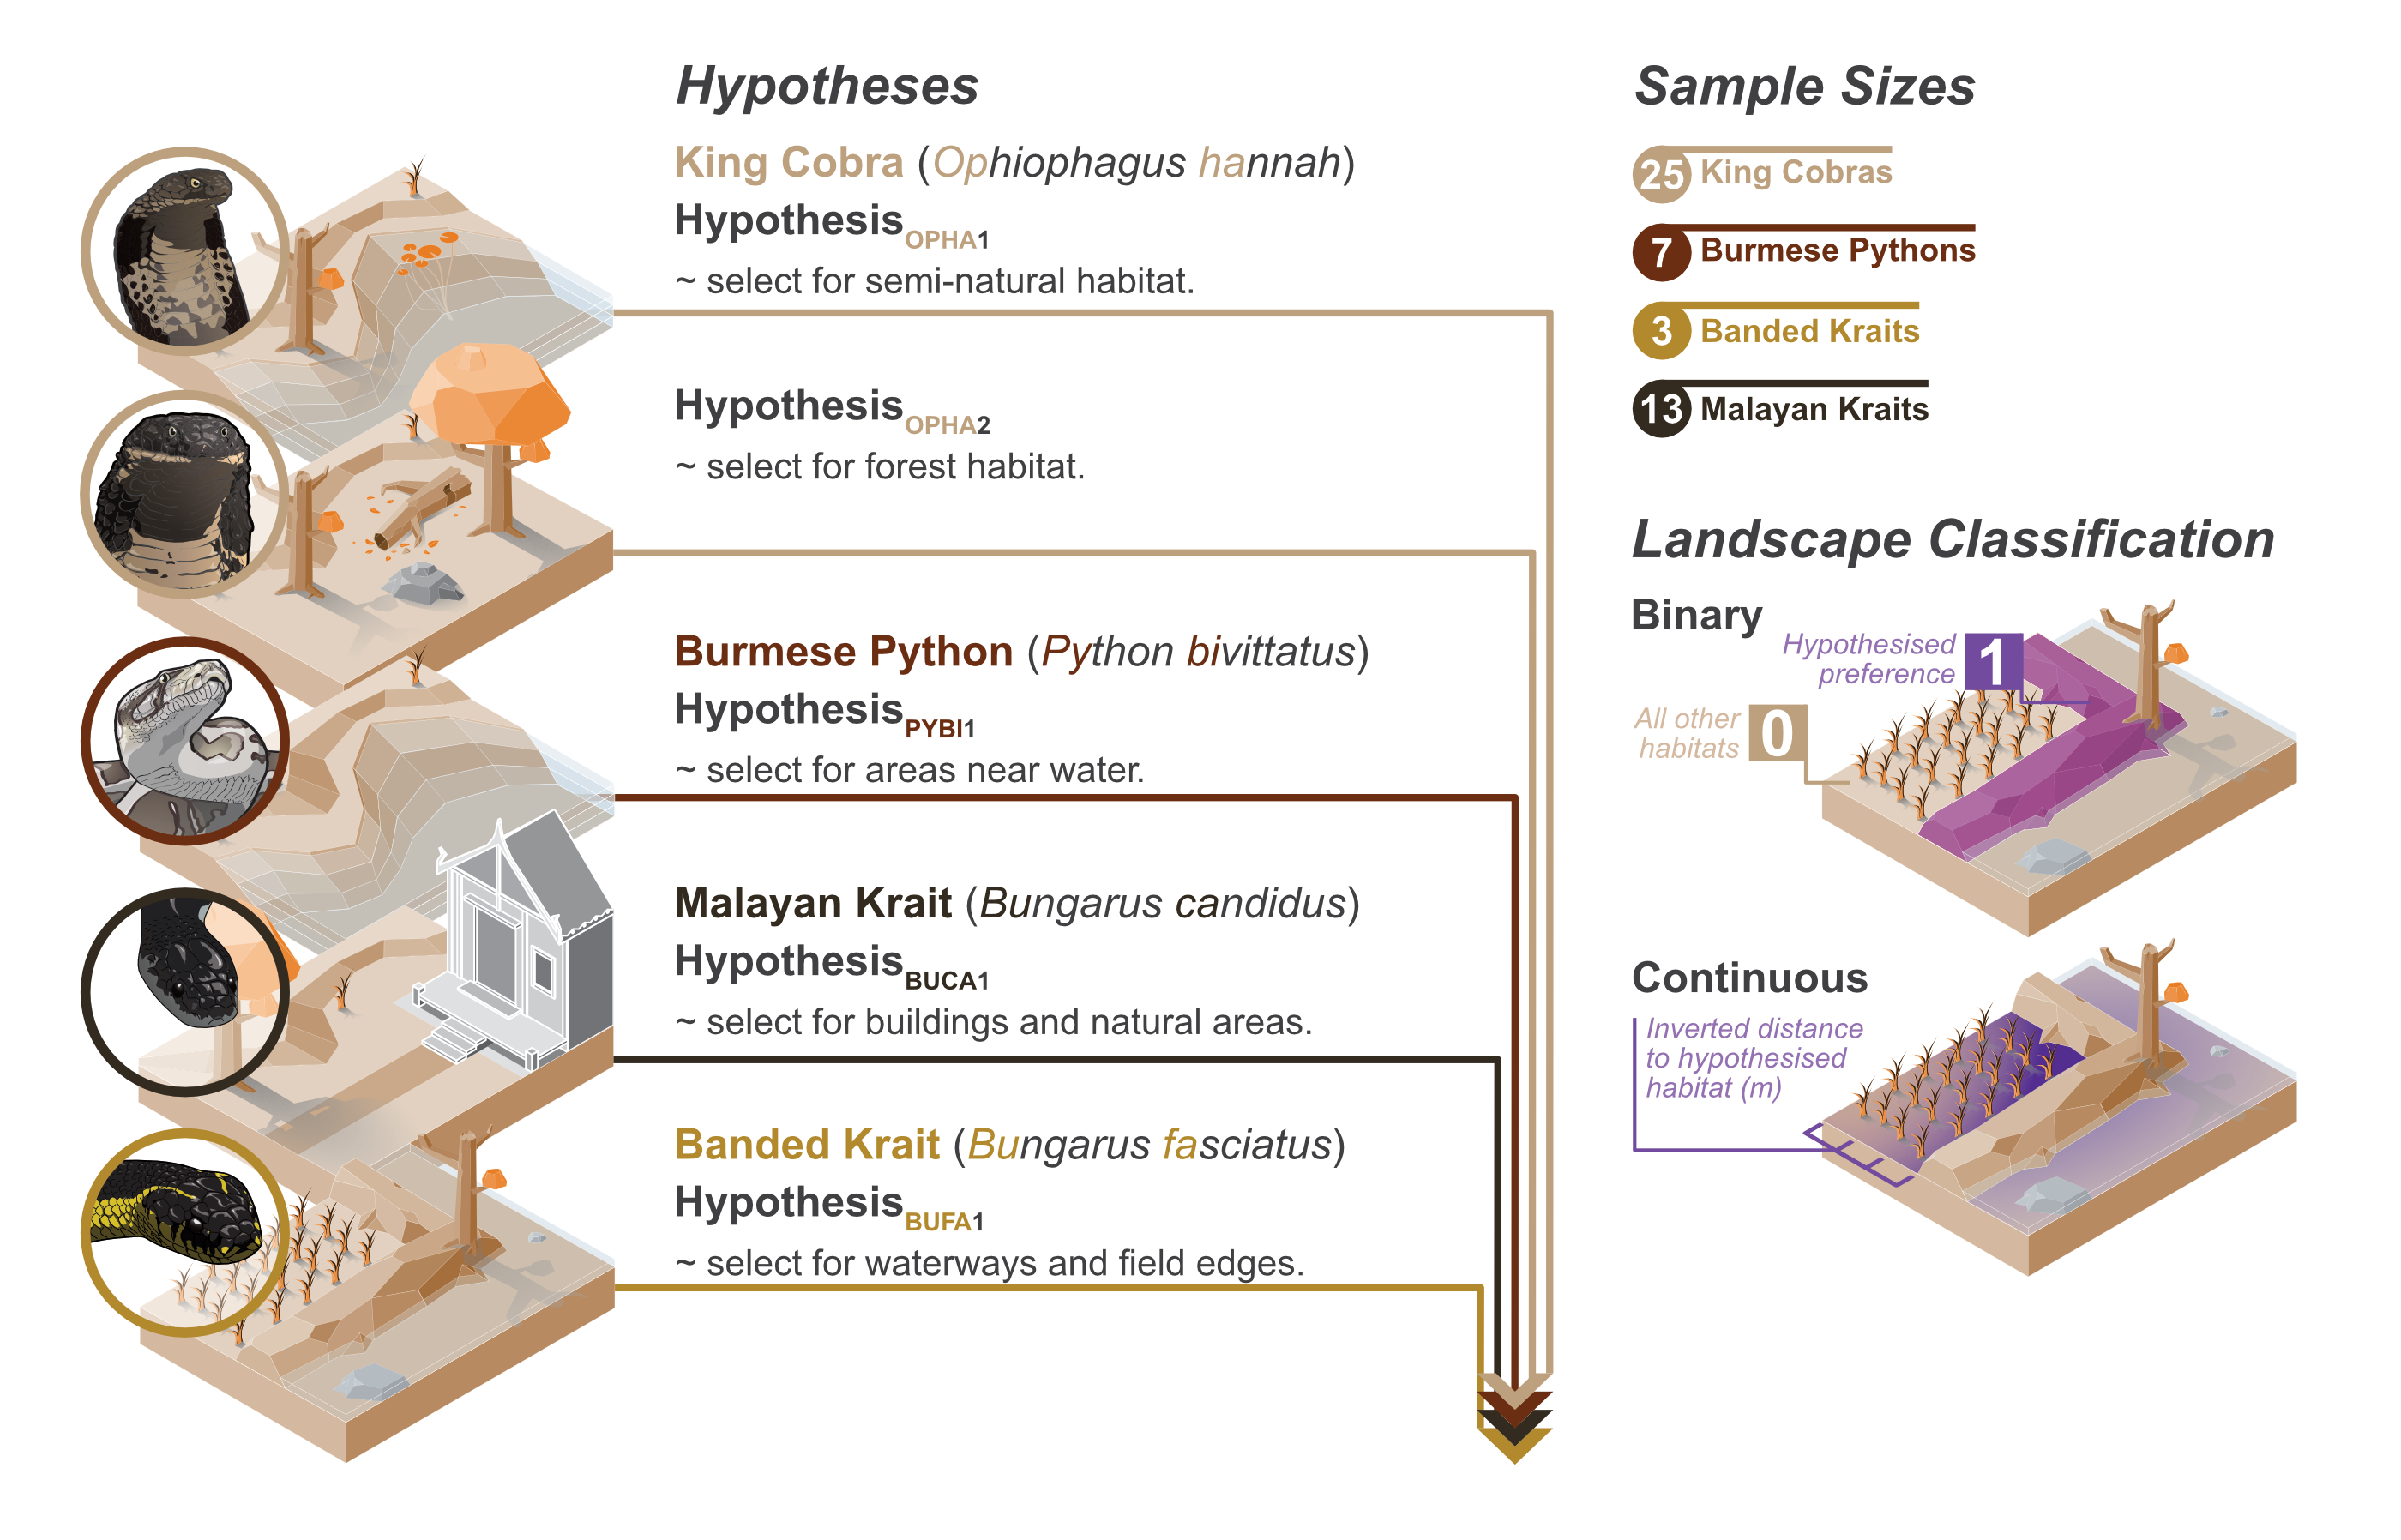
\includegraphics[width=1\linewidth]{../ext_images/hypothesis_visual} \caption{...}\label{fig:hypothesesFigure}
\end{figure}

\subsubsection{King Cobra}\label{king-cobra}

Marshall et al. (\citeproc{ref-Marshall2018}{2019}) and Marshall et al. (\citeproc{ref-marshall_no_2020}{2020a}) are concerned with King Cobras (\emph{Ophiophagus hannah}).
King Cobras are a large (tracked individuals between 1.40 and 3.71m snout to vent length), diurnal, active foraging snake species that depredate snakes and monitor lizards (\citeproc{ref-Jones_supposed_2020}{Jones et al., 2020}).
While considered a predominately forest dwelling species (\citeproc{ref-Stuart2012}{Stuart et al., 2012}), they are known to make use of more human altered areas (\citeproc{ref-Whitaker2004}{Whitaker \& Captain, 2004}; \citeproc{ref-Rao2013}{Rao et al., 2013}; \citeproc{ref-jones_how_2022}{Jones et al., 2022}), which can lead to frequent human-snake conflict (\citeproc{ref-Shankar2013a}{Shankar et al., 2013}; \citeproc{ref-Marshall2018b}{Marshall et al., 2018}).
The extremely low occurrence of King Cobra bites in Thailand means that instances of human-snake conflict are primarily a conservation concern as opposed to human health (\citeproc{ref-Viravan1992}{Viravan et al., 1992}; \citeproc{ref-Pochanugool1998}{Pochanugool et al., 1998}).

Marshall et al. (\citeproc{ref-Marshall2018}{2019}) does not conclude on an actual selection, instead highlighting the King Cobras' excursions out of the protected forest.
Marshall et al. (\citeproc{ref-marshall_no_2020}{2020a}) looks more specifically at selection, highlighting the importance of semi-natural areas that occupy the banks of irrigation canals and intersect the agricultural matrix surrounding the protected forest.
Therefore, we will pool both datasets and examine two non-mutually exclusive hypotheses.

H\textsubscript{OPHA1}: King Cobras select for semi-natural habitat.

H\textsubscript{OPHA2}: King Cobras select for forest habitat.

\subsubsection{Burmese Python}\label{burmese-python}

Smith et al. (\citeproc{ref-smith_native_2021}{2021}) describe Burmese Python (\emph{Python bivittatus}) habitat selection and movement.
Burmese Pythons are large (tracked individuals between 2.21 and 3.09m snout to vent length), ambush predators capable of tacking prey over 100\% their own body mass (\citeproc{ref-bartoszek_natural_2018}{Bartoszek et al., 2018}) and impacting mammal populations (\citeproc{ref-dorcas_severe_2012}{Dorcas et al., 2012}).
The flexibility in regards to prey size means snakes of this size are inevitably drawn into conflict with humans over livestock, a pattern mirrored across the globe for large snakes (\citeproc{ref-Miranda2016}{Miranda, Ribeiro- \& Strüssmann, 2016}).

The conclusions of Smith et al. (\citeproc{ref-smith_native_2021}{2021}) on python habitat selection are not dissimilar to those made on King Cobras, with an active selection for areas near water.
The land classification used in Smith et al. (\citeproc{ref-smith_native_2021}{2021}) was slightly different to Marshall et al. (\citeproc{ref-marshall_no_2020}{2020a}), grouping semi-natural areas with larger water bodies (e.g., agricultural ponds).

H\textsubscript{PYBI1}: Burmese Pythons select for areas near water.

\subsubsection{Malayan Krait}\label{malayan-krait}

Hodges et al. (\citeproc{ref-hodges_malayan_2022}{2022}) examine a smaller species, the Malayan Krait (\emph{Bungarus candidus}).
The Malayan Kraits tracked were between 0.65 and 1.46m snout to vent, and all lived on a university campus.
Malayan Kraits, like many elapids, have a potent and medically significant venom; bites of Malayan Kraits can be fatal (\citeproc{ref-looareesuwan_factors_1988}{Looareesuwan, Viravan \& Warrell, 1988}; \citeproc{ref-searo_regional_office_for_the_south_east_asia_rgo_guidelines_2016}{South East Asia (RGO) \& Asia, 2016}).
They are (mostly) nocturnal and actively foraging (\citeproc{ref-hodges_deadly_2021}{Hodges et al., 2021a}), known to depredate a wide range of prey (\citeproc{ref-kuch_notes_2001}{Kuch, 2001}; \citeproc{ref-hodges_diurnal_2020}{Hodges, D'souza \& Jintapirom, 2020}).

Unlike the other case studies, Hodges et al. (\citeproc{ref-hodges_malayan_2022}{2022}) is undertaken in a more urban environment.
The scale of the Malayan Krait movements meant the study was conducted at a finer spatial scale; habitat types are therefore more finely separated (e.g., buildings vs settlements).
The overall conclusions highlight two habitat types comprising of buildings and natural vegetation are potentially being selected for, in contrast to the lack of selection for open areas.

H\textsubscript{BUCA1}: Malayan Kraits select for buildings and natural areas.

\subsubsection{Banded Krait}\label{banded-krait}

Knierim (\citeproc{ref-knierim_spatial_2019}{2019}) looked at a larger krait species, the Banded Krait (\emph{Bungarus fasciatus}).
Like its smaller cousin, the Banded Krait is also a nocturnal active forager, with a potent venom.
The Banded Krait is heavier-bodied and grows to longer lengths, tracked individuals ranging from 1.13 and 1.58 m snout to vent length.
However, unlike the Malayan Krait, the Banded Krait appears less tolerant of human disturbance in this region of Thailand and tends to have a more ophiophagus diet (\citeproc{ref-Knierim2017a}{Knierim, Barnes \& Hodges, 2017}).

Banded Kraits were entirely located in agricultural land, and like the other krait had movements more conducive to finer habitat classifications.
For example, field margins were found as a key nesting site (\citeproc{ref-knierim_spatial_2019}{Knierim, 2019}).
Knierim (\citeproc{ref-knierim_spatial_2019}{2019}) shows the importance of field margins is reflected in the movement and habitat selection, as Banded Kraits follow the linear water or field margin features as opposed to the wider more exposed field areas.

H\textsubscript{BUFA1}: Banded Kraits select for waterways and field edges.

\subsection{Tracking Data}\label{tracking-data}

We downloaded tracking data from Movebank or linked data repositories associated with the original studies.
The land use data was largely included with the associated data repositories, in cases where it was not we retrieved this from the original authors.
We collated all tracking and land use data, unifying the data formats, naming conventions, and converting files to more accessible formats.
We were left with two files for every study: a csv containing the movements of all individuals, and geoJSON file containing the polygon data describing land use.
The movement data contains seven columns: ``species'' = the binomial species name, ``id'' = the individual animal ID, ``sex'' = whether the individual is male (M) or female (F), ``x'' = the UTM Easting coordinate (m),``y'' = the UTM Northing (m), ``UTMzone'' = the UTM zone either 47N or 48N, ``datetime'' = the date and time formatted as ISO 8601 ``YYYY-MM-DD hh:mm:ss'' recorded in ``Asia/Bangkok''.
The land use data contains geometry data in UTM projection, and data on the ``landuse'' category as well as a ``habitat'' column denoting whether the habitat is part of a hypothesis.

To reacquaint ourselves with the data, and check for any potential issues that could hinder habitat selection analysis, we used code from Crane et al. (\citeproc{ref-crane_lots_2021}{2021}) to generate summaries of all the tracking datasets (code from Crane et al. (\citeproc{ref-crane_supplementary_2020}{2020})).
During this process we identified duplicated data points in the King Cobra data that required removal.
We suspect that these escaped detection during the initial publication (\citeproc{ref-Marshall2018}{Marshall et al., 2019}) because the methods used did not use time in estimation of home range.

\subsection{Multiverse Construction}\label{multiverse-construction}

\begin{verbatim}
## Warning: package 'dplyr' was built under R version 4.2.3
\end{verbatim}

\begin{verbatim}
## 
## Attaching package: 'dplyr'
\end{verbatim}

\begin{verbatim}
## The following objects are masked from 'package:stats':
## 
##     filter, lag
\end{verbatim}

\begin{verbatim}
## The following objects are masked from 'package:base':
## 
##     intersect, setdiff, setequal, union
\end{verbatim}

\begin{verbatim}
## Warning: package 'stringr' was built under R version 4.2.3
\end{verbatim}

To explore the variation that could arise when testing the above hypotheses, we constructed a multiverse of analytical choices.
A multiverse is tree of branching paths, where decisions made during analysis spawn multiple branches, each with alternative answers.
Previous work has reveal the importance of data quantity over analysis decisions in determining habitat selection (\citeproc{ref-marshall_habitat_2024}{Marshall \& Duthie, 2024}) (Chapter 3), but we are still left with sizeable variation in final answers --and perhaps more importantly answers that offer contradictory conclusions.
The variation in results are similarly present in more practical demonstrations, such as many analysts projects (\citeproc{ref-gould_same_2023}{Gould et al., 2023}).

\begin{figure}
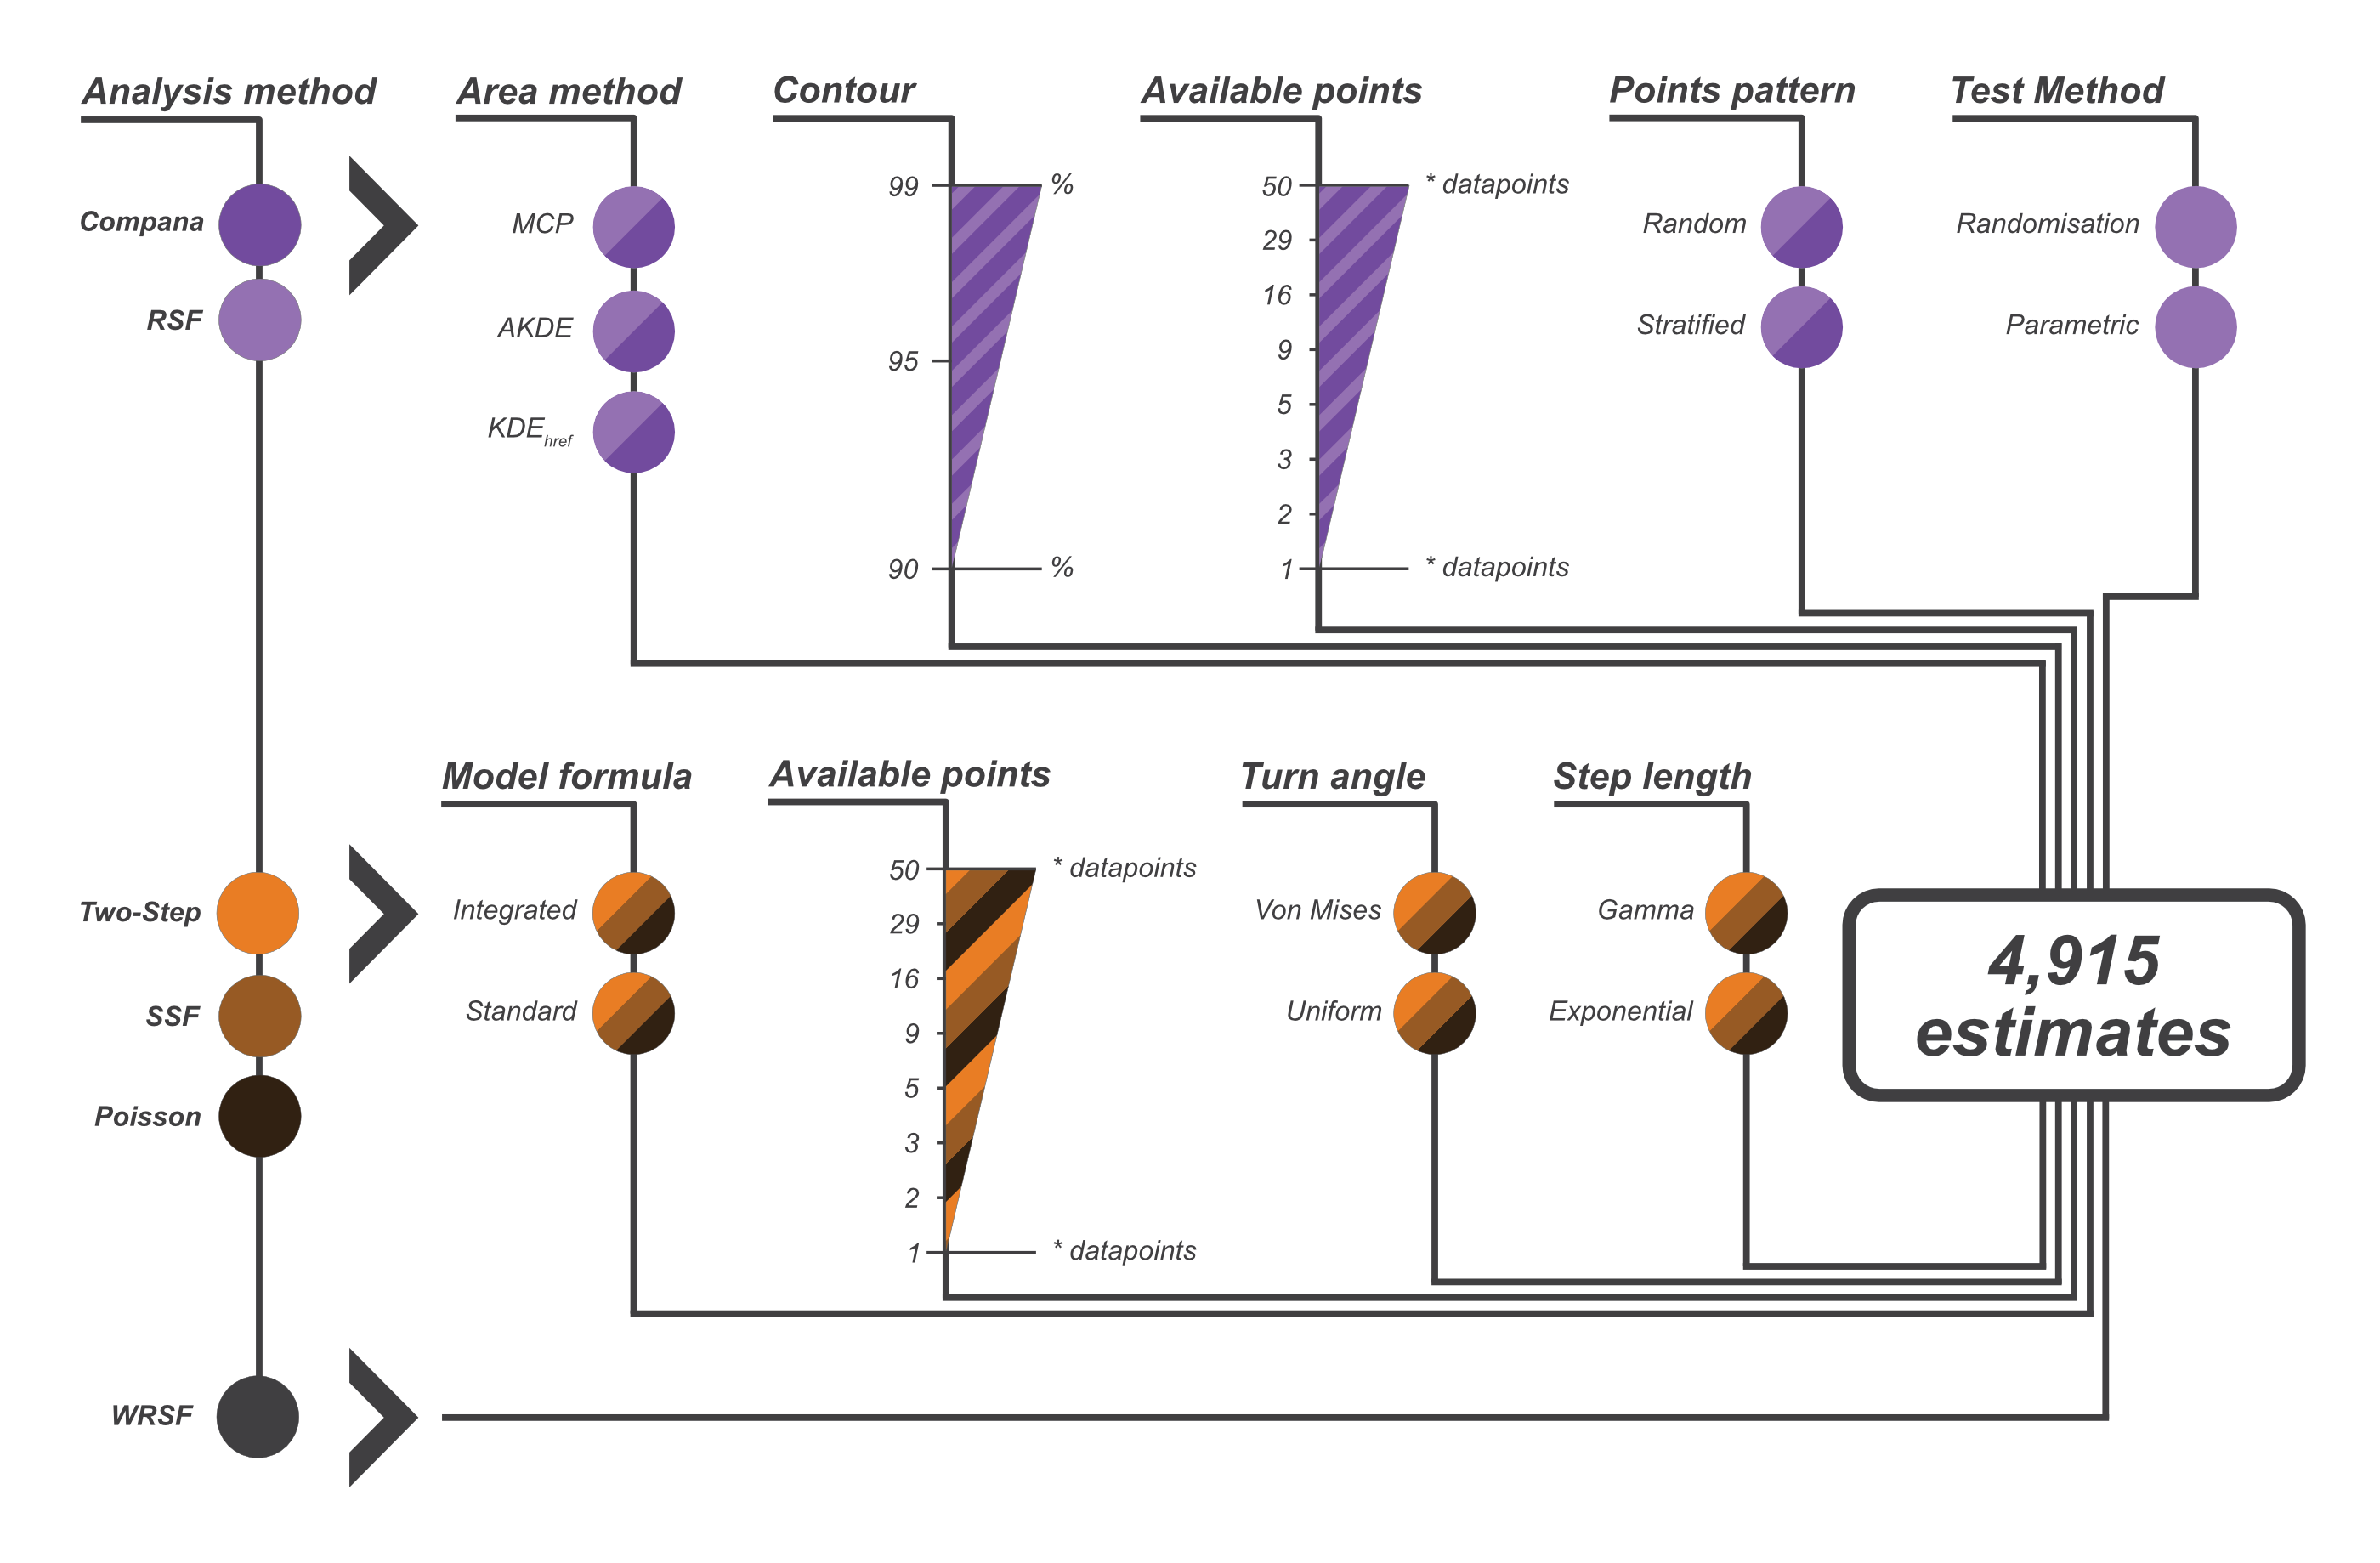
\includegraphics[width=1\linewidth]{../ext_images/decisions_visual} \caption{...}\label{fig:decisionsFigure}
\end{figure}

Our multiverse starts with two alternative ways of defining the habitats.
Each case study has a map of available habitats, defined as categories.
One approach we used is to examine the habitat selection by retaining these categories, only simplifying them to fit the hypotheses.
This simplification took the habitat(s) of interest and codes them as 1, whereas all other habitats previously indicated in the studies to be avoided/not-selected for are coded as 0 (Fig. \ref{fig:landscapePlotOPHA1}; Fig. \ref{fig:landscapePlotOPHA2}; Fig. \ref{fig:landscapePlotPYBI1}; Fig. \ref{fig:landscapePlotBUCA1}; Fig. \ref{fig:landscapePlotBUFA1}).
For example, in the case of Malayan Kraits, buildings and natural areas were classed as 1, and all other types classed as 0.
We then used the 0/1 classification as a predictor in the habitat selection analyses.
We undertook this simplification to facilitate the repeated use of generic code in the multiverse.
The second approach involved converting the simplified categorical habitat types into continuous rasters, where each cell described the distance to a given habitat type.
We inverted the distances (and scaled), so that a positive effect in the model mean a positive selection towards a habitat type, resulting in a more intuitive final output (Fig. \ref{fig:landscapePlotOPHA1}; Fig. \ref{fig:landscapePlotOPHA2}; Fig. \ref{fig:landscapePlotPYBI1}; Fig. \ref{fig:landscapePlotBUCA1}; Fig. \ref{fig:landscapePlotBUFA1}).
All analyses (see below) were run on both classifications, with the exception of the Compositional Analysis that required categoric inputs.

The habitat selection methods we explored consisted of: Resource Selection Functions (RSF) and Composite Analysis (Compana) that we called area-based methods, which used an estimated available area to help define availability for the snakes; Step Selection Functions (SSF), Two-Step (Two-Step), and Poisson models (Poisson) that we refer to as step-based methods, which used randomly generated alternative locations based on the movement and sinuosity of the individual being examined; and a newly described weighted Resource Selection Functions (wRSF), which use a fitted movement model to calibrate the available habitat.

The area-based category made use of a defined area of availability, for which random available points can be drawn.
To explore the impact of the definition of available, we created a number of different polygons surrounding the tracking data locations.
We created available areas using Minimum Convex Polygons (MCP), Kernel Density Estimates (KDE: using the reference smoothing bandwidth {[}href{]}), and Autocorrelated Kernel Density Estimates (aKDE).
We used the adehabitatHR for MCP and KDE creation (\citeproc{ref-adehabitatHR}{Calenge \& Scott Fortmann-Roe, 2023}), and the ctmm package for aKDEs (\citeproc{ref-Fleming2015}{Fleming et al., 2015}; \citeproc{ref-Calabrese2016}{Calabrese, Fleming \& Gurarie, 2016}; \citeproc{ref-Fleming2017}{Fleming \& Calabrese, 2017}, \citeproc{ref-ctmm}{2023}).
For the aKDEs we fitted a number of movement models: Ornstein-Uhlenbeck (OU), Ornstein--Uhlenbeck Foraging (OUF), and Independent Identically Distributed (IID); we selected the best performing by AICc.
We elected to follow guidance from (\citeproc{ref-silva_autocorrelationinformed_2022}{Silva et al., 2022}), opting for weighted aKDEs and the perturbative hybrid residual maximum likelihood method (pHREML).
The weighted AKDEs are better suited for tracking data with gaps.
All three methods require an outer most contour to be selected to define the edge of the available habitat; we varied this outer edge including analysis of 90, 95, and 99\% contours.
For the aKDE areas, we selected the point estimate connected to the contour percentage, ignoring the 95\% confidence intervals associated with the estimate.

Once an available area was defined, we generated points within the area to extract the available habitat (also referred to as available points).
We varied the point generation process, either purely random or stratified across the overall area.
In addition to the point generation method, we varied the the number of available points by multiplying the number of known/used data points by 1 to 50.
As each individual had their own available area, we explored Type III habitat selection; this kept this analysis closer to the intent of the original publications.

The step-based models, instead of using an available area, use available steps randomly generated for each time step.
For these step-based methods a different suite of choices were explored.
First is the number of random steps generated per known location, we ranged this from 1 to 50.
To generate those steps we draw values from distributions, the choice of those distributions make up the next two choices.
For the random step lengths we looked at impact of using Gamma and Exponential distributions; whereas for the turn angles we looked at Von Mises and Uniform distributions.
Once the random available locations had been generated, we explore an additional choice regarding the model formula: whether to have the step lengths and turn angles interact with the habitat.
Termed integrated step-selection, the inclusion of the step lengths and turn angles is meant to aid the acquisition of less biased estimates of habitat selection.
However, the impacts of the inclusion have differing impacts when using step-selection or a Poisson model (see Chapter 3); we include it here to explore how dramatic that difference can be.
While the Poisson models explicitly target population level selection, the SSF models required summation to a single value.
To generate that value, we conducted a simple mean of the point estimates and calculated corresponding 95\% confidence intervals.
This process likely underestimates the overall uncertainty surrounding the SSF methods, as the uncertainty surrounding the initial estimates is lost.

We also used the newly developed wRSF methods (\citeproc{ref-alston_mitigating_2023}{Alston et al., 2023}).
This approach dramatically reduces the choices during analysis; instead of requiring a defined area of availability, the wRSF weights individual animal locations (their impact penalised by repeated information resulting from autocorrelation) and compares them against a range distribution taking the form of a weighted AKDE (\citeproc{ref-alston_mitigating_2023}{Alston et al., 2023}).
Once the movement models had been generated, and wRSF models fitted, we used the supplied mean functionality within the ctmm package to generate an overall population selection.

We handled the running of all analyses and their associated choices using the targets v.1.6.0 and tarchetypes v.0.9.0 R packages (\citeproc{ref-targets}{Landau, 2021a},\citeproc{ref-tarchetypes}{b}).
These packages allowed for efficient parallel process and tracking of intermediate objects while avoiding errors in one analysis pathway from delays the completion of others.

During the running of the multiverse there were several instances of model fitting issues.
\emph{Ophiophagus hannah} 002, 004, and 005 had issues with step lengths fitting to a exponential distribution; we addressed this by excluding the top 25\% quantile of observed steps when the exponential fit failed.
One \emph{Bungarus candidus} individual did not have sufficient relocations to generate any area estimates; therefore we excluded them.
There were infrequent instances where individuals did not enter both habitat types (or available points did not cover both types made more likely with fewer available points); this caused issues with model fitting in Two-Step and SSF approaches.
We re-ran random step generation for those individuals to maximise the chances that available points captured both habitat types.
If the convergence failed persisted, we excluded those individuals from that habitat selection estimate end-point.

\subsection{Bayesian meta-analysis}\label{bayesian-meta-analysis}

We ran a series of 45 Bayesian meta-analysis models to determine an overall estimate of habitat selection for each analysis approach and hypothesis.
We used the following model formula: ``estimate''\textbar se(``estimate confidence'') \textasciitilde{} 1 + ``choices'' + (1\textbar{}``index of analysis end point'').
The estimate confidence measure varied from method to method: area-based Compana did not have a confidence interval so we excluded that term, for the RSF and Two-Step estimates we used standard error, for the SSF models we used standard errors of the model averaging, and for the Poisson models we used the standard deviation.
Choices varied per method, and included a term for every choice made to reach a given analysis end point.
For the area-based methods (Compana, RSF) the choice terms included area method MCP, AKDE, KDEhref, contour percentage (90, 95, 99, scaled), available points generation method (random, stratified), and the number of available points generated per animal location (1 to 50, scaled).
The Compana analysis had the additional choice of test method (randomisation, parametric).
For the step-based methods (Two-Step, SSF, Poisson) the choice terms included model formula (integrated, non-integrated), step length distribution (Gamma, Exponential), turn angle distribution (Von Mises, Uniform), and the number of random steps generated per animal location (Inf to -Inf, scaled).
We used weakly informative priors.
For the intercept prior we used a normal distribution with a mean of 0 and a standard deviation of 2, and for the choices' priors we used Cauchy distributions with a location of -0.1 and scale as 3, except for the number of available points generated per animal location where we used a location of 0.1.
We ran Bayesian models using the brms package (\citeproc{ref-brms}{Bürkner, 2021}), running 4 MCMC chains for 1200 iterations each, with a warmup of 400, and a thinning rate of 2.
For reporting we used 95\% median highest density continuous intervals when describing posteriors.

\section{Results}\label{results}

\subsection{Tracking Summary}\label{tracking-summary}

Sample sizes and data density varied between species and individuals.
We tracked 25 king cobras, 7 Burmese Pythons, 13 Malayan Kraits, and 3 Banded Kraits, which had adequate data for analysis (Fig. \ref{fig:timeLinePlot}).
Tracking duration ranged widely from 37 to 1176 days (Table. \ref{tab:trackingSummaryTable}), being cut short by snake deaths, transmitter failure, and studies ending.
On average we tracked an individual snake for 281.37 ±SD 246.33 days.
Despite best efforts to maintain a consistent tracking regime, snakes evade rediscover, weather prevents tracking, and equipment fails.
Therefore, all species tend to have mean tracking lag times (i.e., the time between subsequent relocations) a little longer than intended (Fig. \ref{fig:timeLagPlot}; Table. \ref{tab:trackingSummaryTable}).
Overall tracking effort resulted in 26,778 data points, across 48 snakes, resulting in a mean of 557.88 ±SD 657.82 per snake.

Activity and propensity to movement varied between the species.
We recorded the most moves for King Cobras (273.28 ±SE 47.86), to due to their more intensive tracking regime.
The other species had on average fewer recorded moves per individual, with Burmese Pythons making on average 112.43 ±SE 33.79 moves, followed by Banded Kraits with 86.67 ±SE 38.18, and finally the more stationary Malayan Kraits with 28.54 ±SE 3.95.

\subsection{Summarising Hypothesis Support}\label{summarising-hypothesis-support}

The area-based Compositional analysis appeared to provide majority support for three of five of our hypotheses: \emph{Ophiophagus hannah} H1, \emph{Bungarus candidus} H1, and \emph{Bungarus fasciatus} H1 (Fig. \ref{fig:specCurveArea}).
In contrast, \emph{Ophiophagus hannah} H2 and \emph{Python bivittatus} H1 hypotheses appeared almost entirely unsupported, with zero or one analysis end point resulting in significant support (Fig. \ref{fig:specCurveAreaOPHA}; \ref{fig:specCurveAreaPYBI}).
The lack of support does not appear to be connected to any single analysis decision.
\emph{Ophiophagus hannah} H2 and \emph{Python bivittatus} H1 hypotheses appear more likely to supported when using MCPs to define available area, and least likely when defined via AKDEs, but even using MCPs there is not consistent support in the point estimates.
High outlying support in \emph{Python bivittatus} H1 estimates are by limited extremely limited numbers of available points.
Also the other species see that available area method and contour have varying impacts.
Only the Compana test method (randomisation or parametric) appears to have a consistent effect, with both \emph{Bungarus} hypotheses seeing dramatically higher estimates of selection when parametric testing is used.
For \emph{Bungarus candidus} this does would not change any conclusions (all estimates are significantly supportive; Fig. \ref{fig:specCurveAreaBUCA}); however, for \emph{Bungarus fasciatus} this single decision is what is responsible for the half of estimates providing support (Fig. \ref{fig:specCurveAreaBUFA}).

\begin{figure}
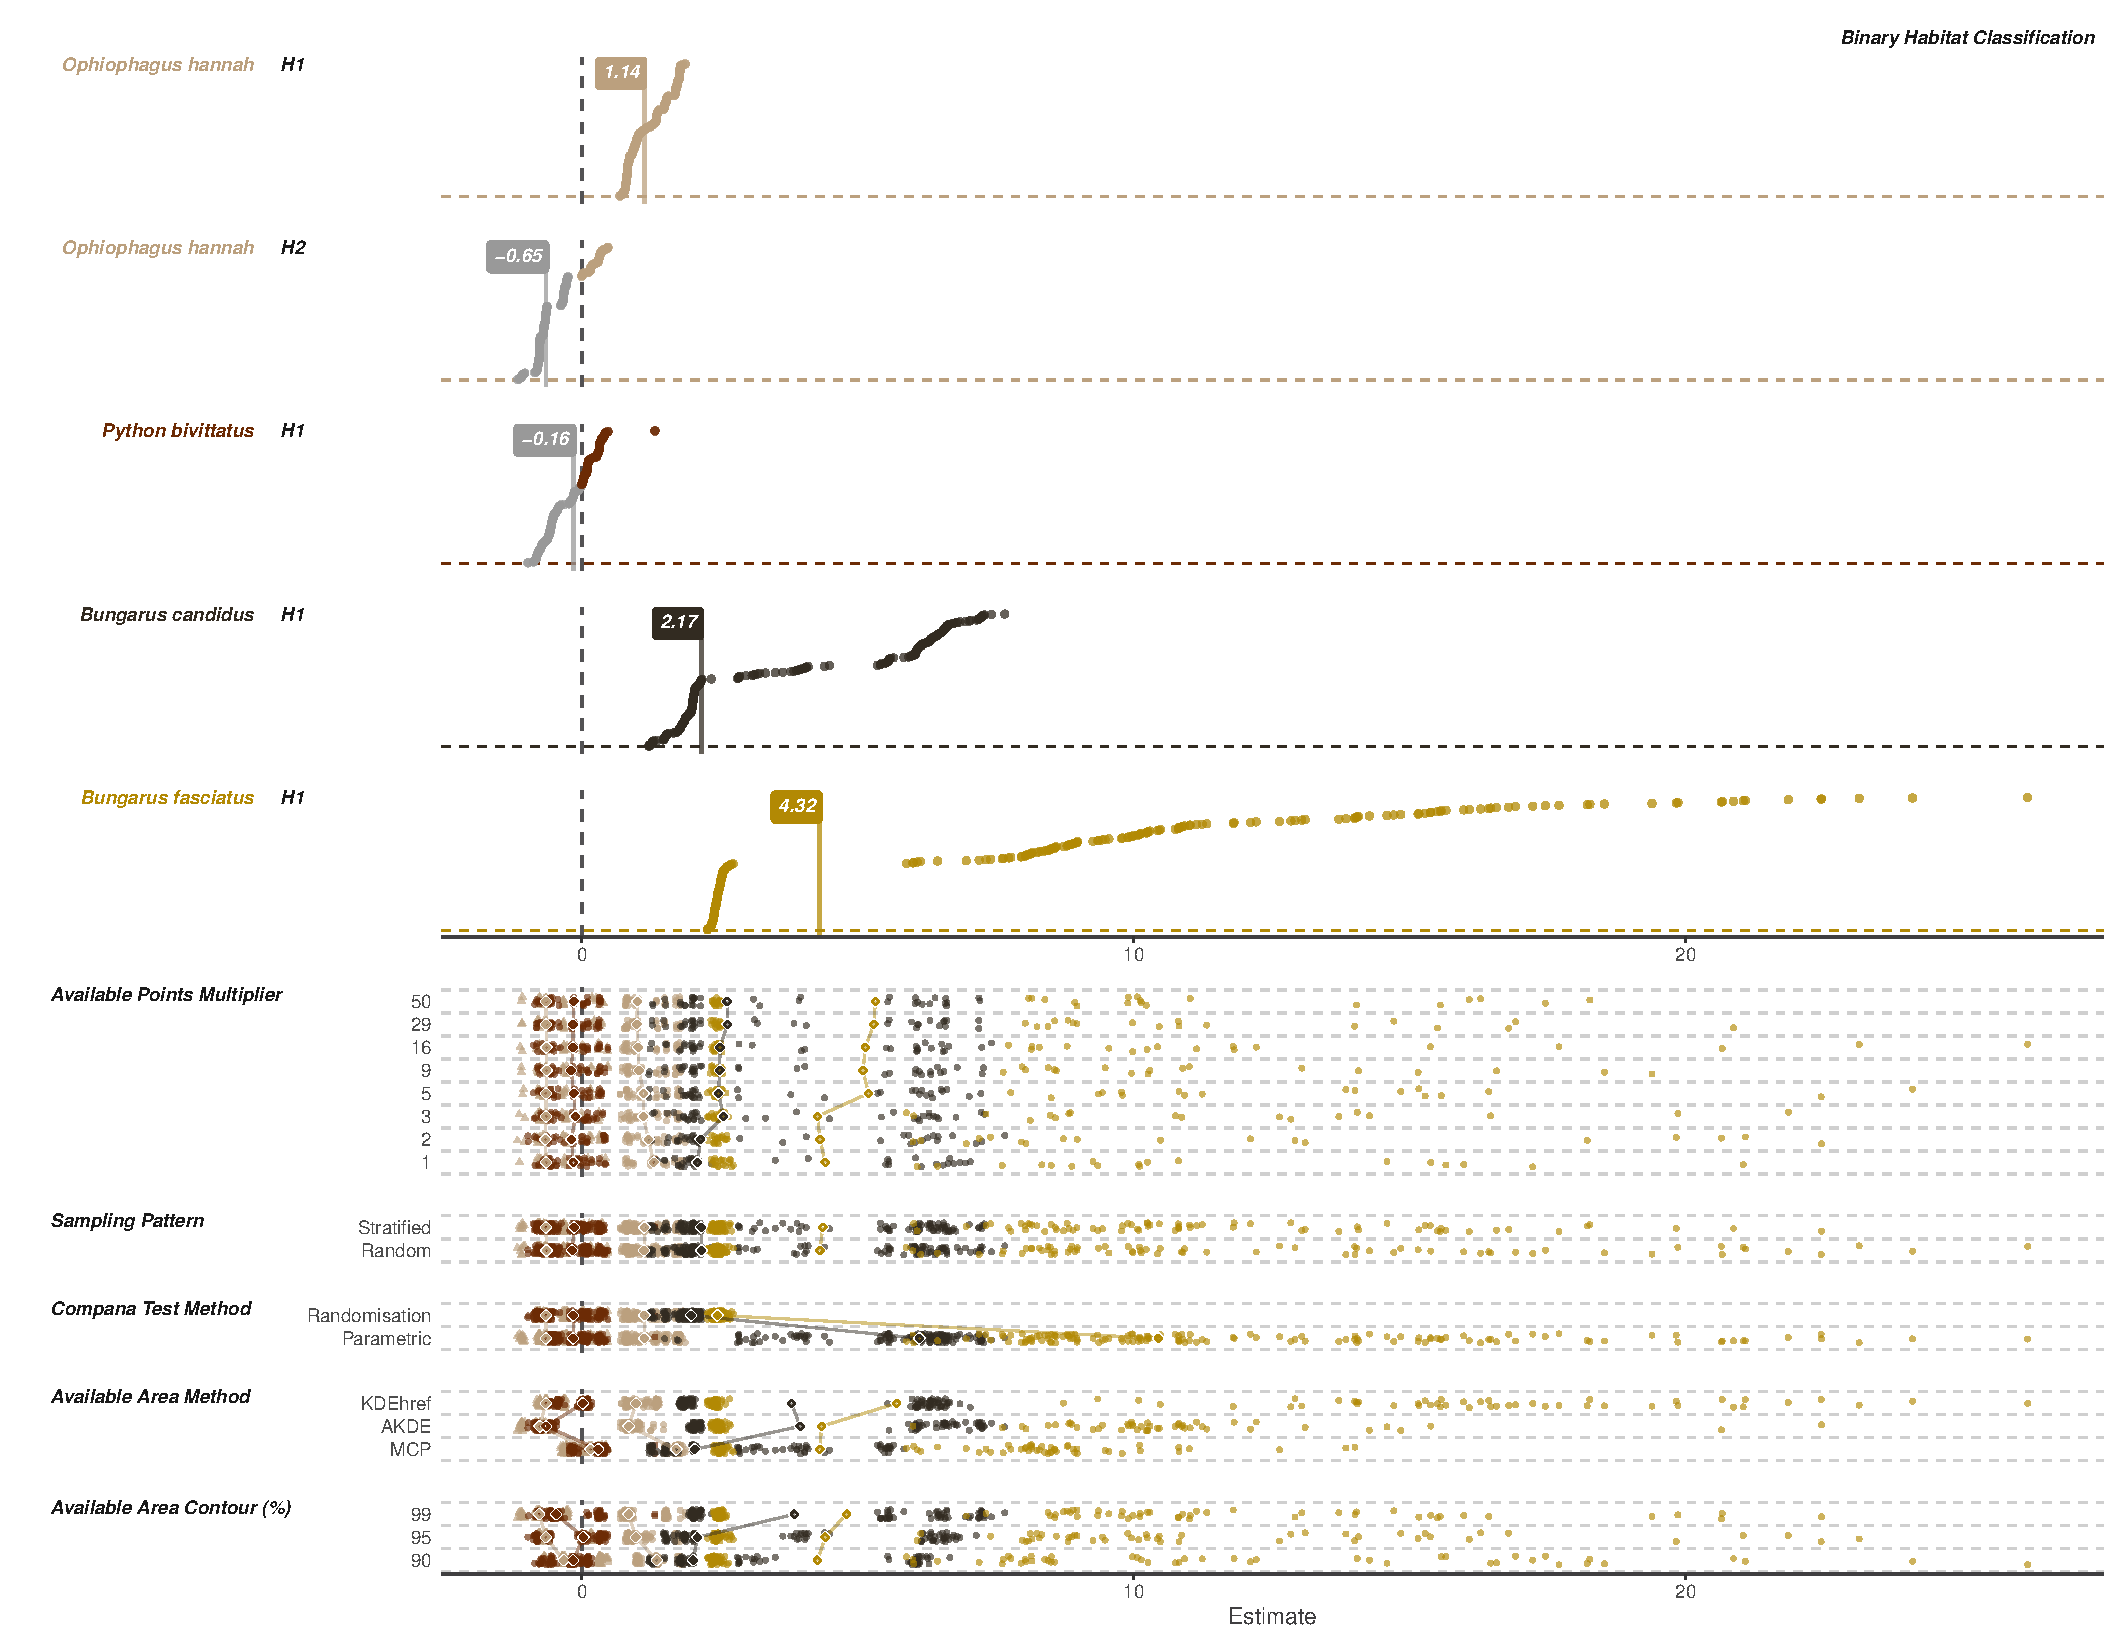
\includegraphics[width=1\linewidth]{../../figures/specCurve_area} \caption{All estimates of habitat selection derived from the areas-based Compositional (Compana) analysis. Top curves show all estimates, split by species and hypothesis, with coloured points indicating those with point estimates supporting the hypothesis (i.e., > 0). Labelled vertical lines show the median estimate for each species-hypothesis combination. Lower plot show the estimates relative to each analysis choice. The colours depict the species, and shape separate hypothesis 1 and 2 for the King Cobras (circles = hypothesis 1, triangle = hypothesis 2). Median estimates are shown with hollow diamonds, and species-hypothesis medians are connected with appropriated coloured lines.}\label{fig:specCurveArea}
\end{figure}

Unlike the Compositional analysis, Resource Selection Functions estimate medians provided support for all hypothesis (Fig. \ref{fig:specCurveRsf}).
Although, \emph{Ophiophagus hannah} H2's support is marginal.
The more limited support for \emph{Ophiophagus hannah} H2 (for both habitat classification methods) appears driven by those estimates based on MCP available areas, and using wider contours (Fig. \ref{fig:specCurveRsfOPHA}).
All other hypotheses are universally supported, and significantly so (with the exception of only six of 144 \emph{Python bivittatus} estimates).
The chosen available area method does appear to impact the variability of results, even among the positive selection estimates.
Those based on MCPs appears to be less variable regardless of other analysis decisions, but this pattern only exists when a continuous habitat classification was used.
The continuous habitat classification does appear to open the possibility for more dramatic variation in selection strength.
The number of available points does seem to impact the estimates in both \emph{Bungarus} species, but only when not using MCPs, and this impact appears to diminish once over 29.

\begin{figure}
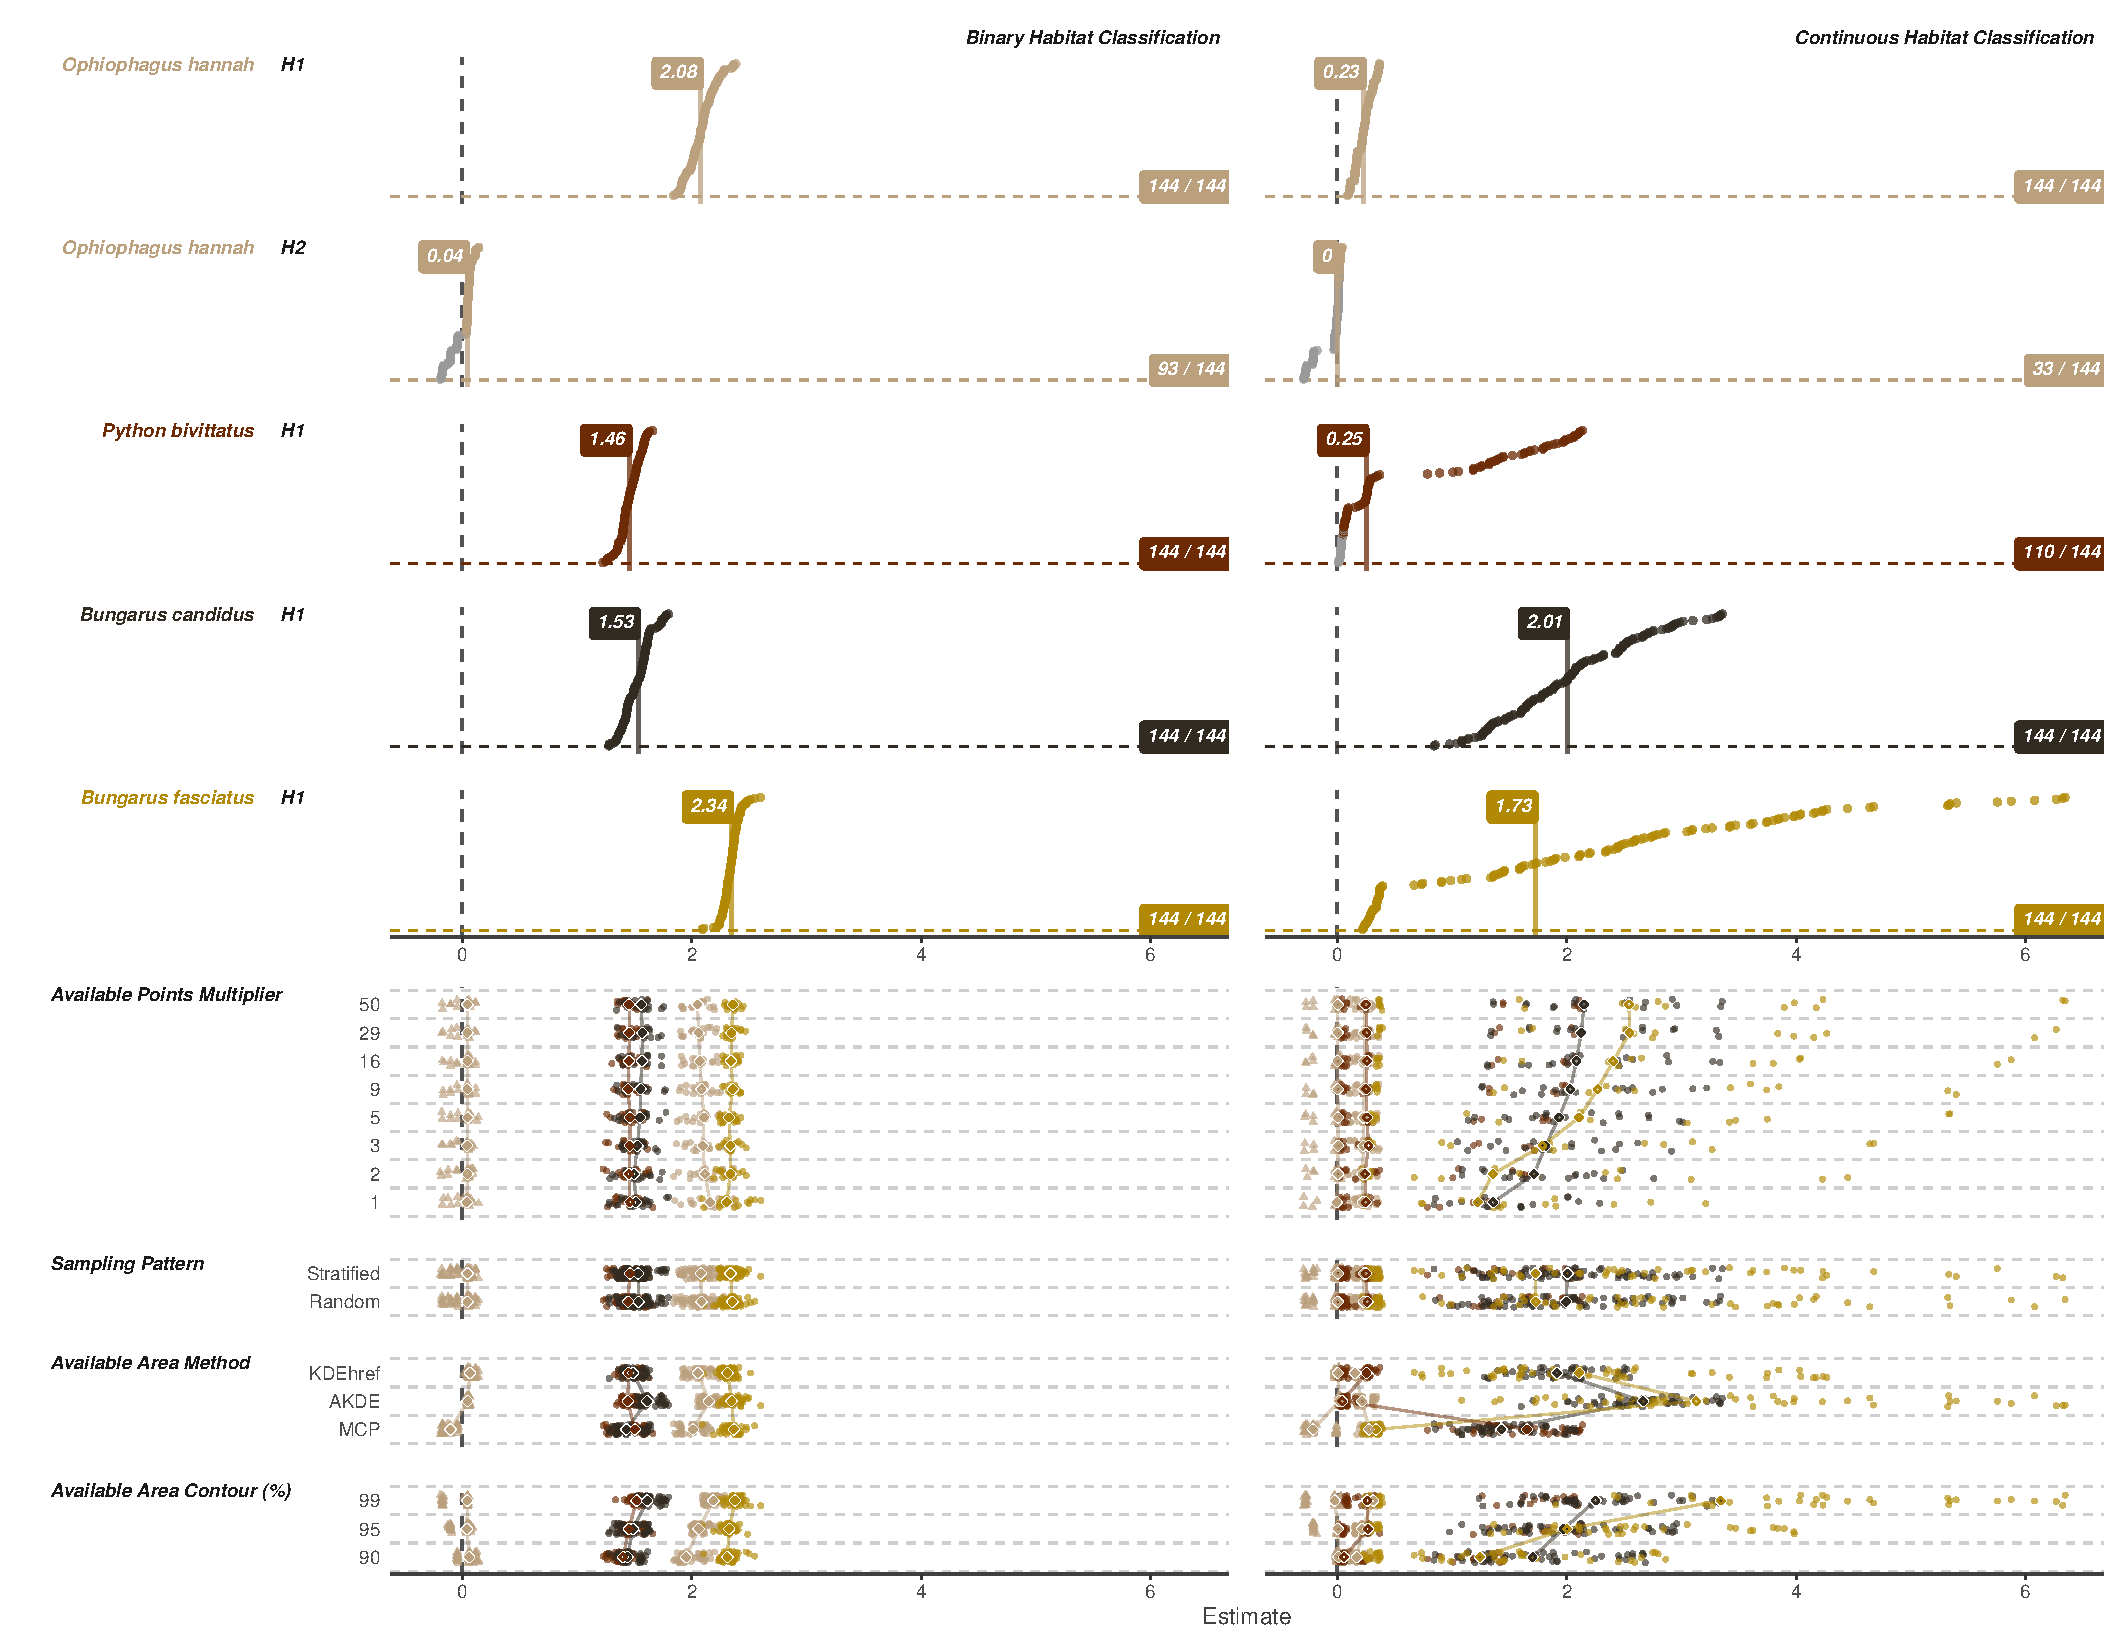
\includegraphics[width=1\linewidth]{../../figures/specCurve_rsf} \caption{All estimates of habitat selection derived from the areas-based Resource Selection Function (RSF) analysis. Top curves show all estimates, split by species and hypothesis, with coloured points indicating those with point estimates supporting the hypothesis (i.e., > 0). Labelled vertical lines show the median estimate for each species-hypothesis combination. Lower plot show the estimates relative to each analysis choice. The colours depict the species, and shape separate hypothesis 1 and 2 for the King Cobras (circles = hypothesis 1, triangle = hypothesis 2). Median estimates are shown with hollow diamonds, and species-hypothesis medians are connected with appropriated coloured lines. The plot is split left and right for the analysis using a binary classification (left), and continuous inverted distance (right).}\label{fig:specCurveRsf}
\end{figure}

The Two-Step approach was by far the least effective and most problematic when running in within a multiverse, as the models had frequent convergence issues.
This failure rate is particularly visible in the \emph{Ophiophagus hannah} data, when ran with low numbers of available points or with attempts to integrate step and turn angle into the equation (Fig. \ref{fig:specCurveTwoStep}).
In addition to the failure rate, we see a more even spread of estimates that contrasts with the ideal ``S'' shape that would indicate more agreement between the analysis end points.
The lack of agreement in selection strength appears more prevalent when using the continuous habitat classification, but unlike with RSFs increased variably does not appear connected to any single choice.
The most consistent impact of the choice is whether to integrate step and turn angle into the model formula.
As mentioned this led to convergence issues for \emph{Ophiophagus hannah}, but for other species the integrated formulations tended to result in more conservative estimates of selection.
Only for \emph{Bungarus candidus} with a binary classification did the median estimate swap direction due to this analysis choice, and explains the lower rates of significant selection (32/64; Fig. \ref{fig:specCurveTwoStepBUCA}).

\begin{figure}
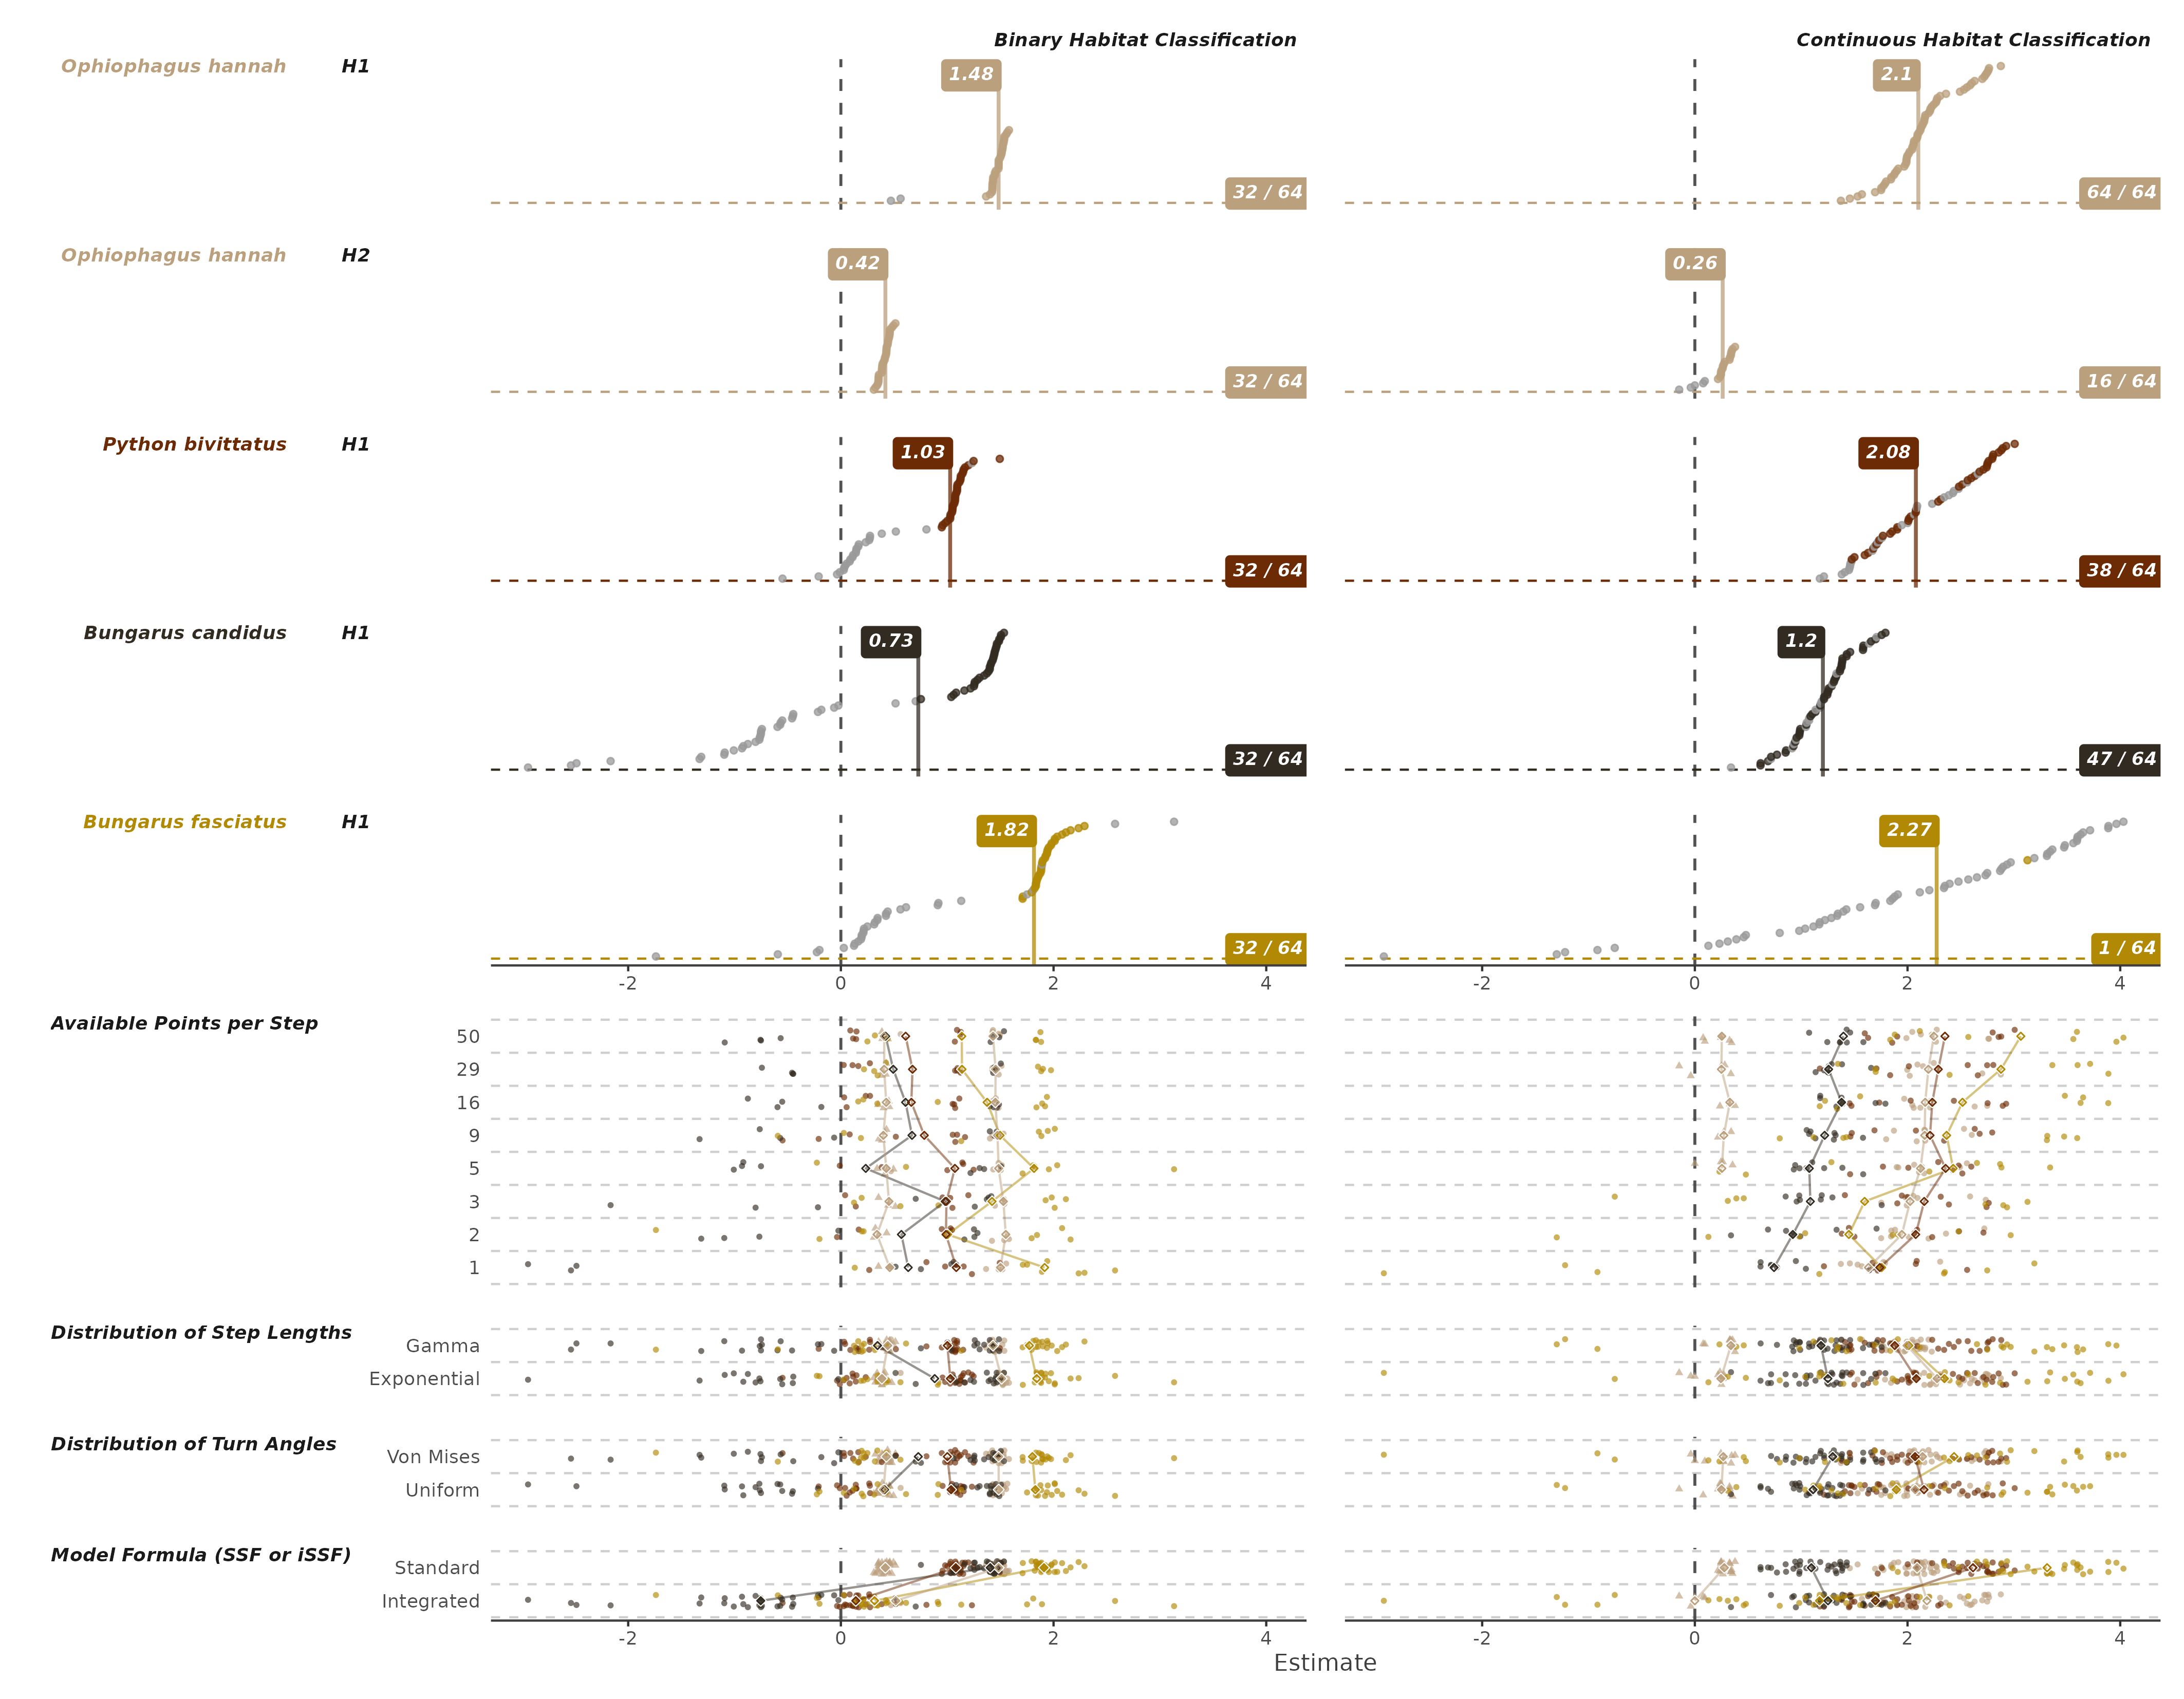
\includegraphics[width=1\linewidth]{../../figures/specCurve_twoStep} \caption{All estimates of habitat selection derived from the step-based Two-Step analysis. Top curves show all estimates, split by species and hypothesis, with coloured points indicating those with point estimates supporting the hypothesis (i.e., > 0). Labelled vertical lines show the median estimate for each species-hypothesis combination. Lower plot show the estimates relative to each analysis choice. The colours depict the species, and shape separate hypothesis 1 and 2 for the King Cobras (circles = hypothesis 1, triangle = hypothesis 2). Median estimates are shown with hollow diamonds, and species-hypothesis medians are connected with appropriated coloured lines. The plot is split left and right for the analysis using a binary classification (left), and continuous inverted distance (right).}\label{fig:specCurveTwoStep}
\end{figure}

The Step Selection Function approach was impacted by the habitat classification method (Fig. \ref{fig:specCurveSsf}).
When using a binary habitat classification on the \emph{Bungarus} analysis supported the hypotheses, whereas we see more universal support when using the continuous habitat classification.
This lack of support when using the binary classification was not clearly connected to any particular analysis decision.
The only decision that makes consistent change when paired with binary classification was the number of available steps.
Increased steps tended to lower the overall variability of selection estimates, especially for \emph{Bungarus candidus}.
While we did see near universal support for hypotheses in the continuous classification, the estimates for \emph{Python bivitattus} were more marginal with only 22 of 64 considered significant support (Fig. \ref{fig:specCurveSsfPYBI}).
We should be additionally cautious with this support, as the SSF model averaging method may be reducing the uncertainty present in individual SSF models.
The impact of decisions are most visible in \emph{Bungarus candidus}, whose estimates' strength is impacted by the step and turn angle distributions, as well as whether the formula was integrated.
The distribution choices make less of an impact, with the spread of estimates largely overlapping, but using an integrated model formula led to more generous and variable estimates of preference.
However, despite this impact, all bar one of \emph{Bungarus candidus} estimates significantly support the hypothesis regardless of habitat classification method (Fig. \ref{fig:specCurveSsfBUCA}).

\begin{figure}
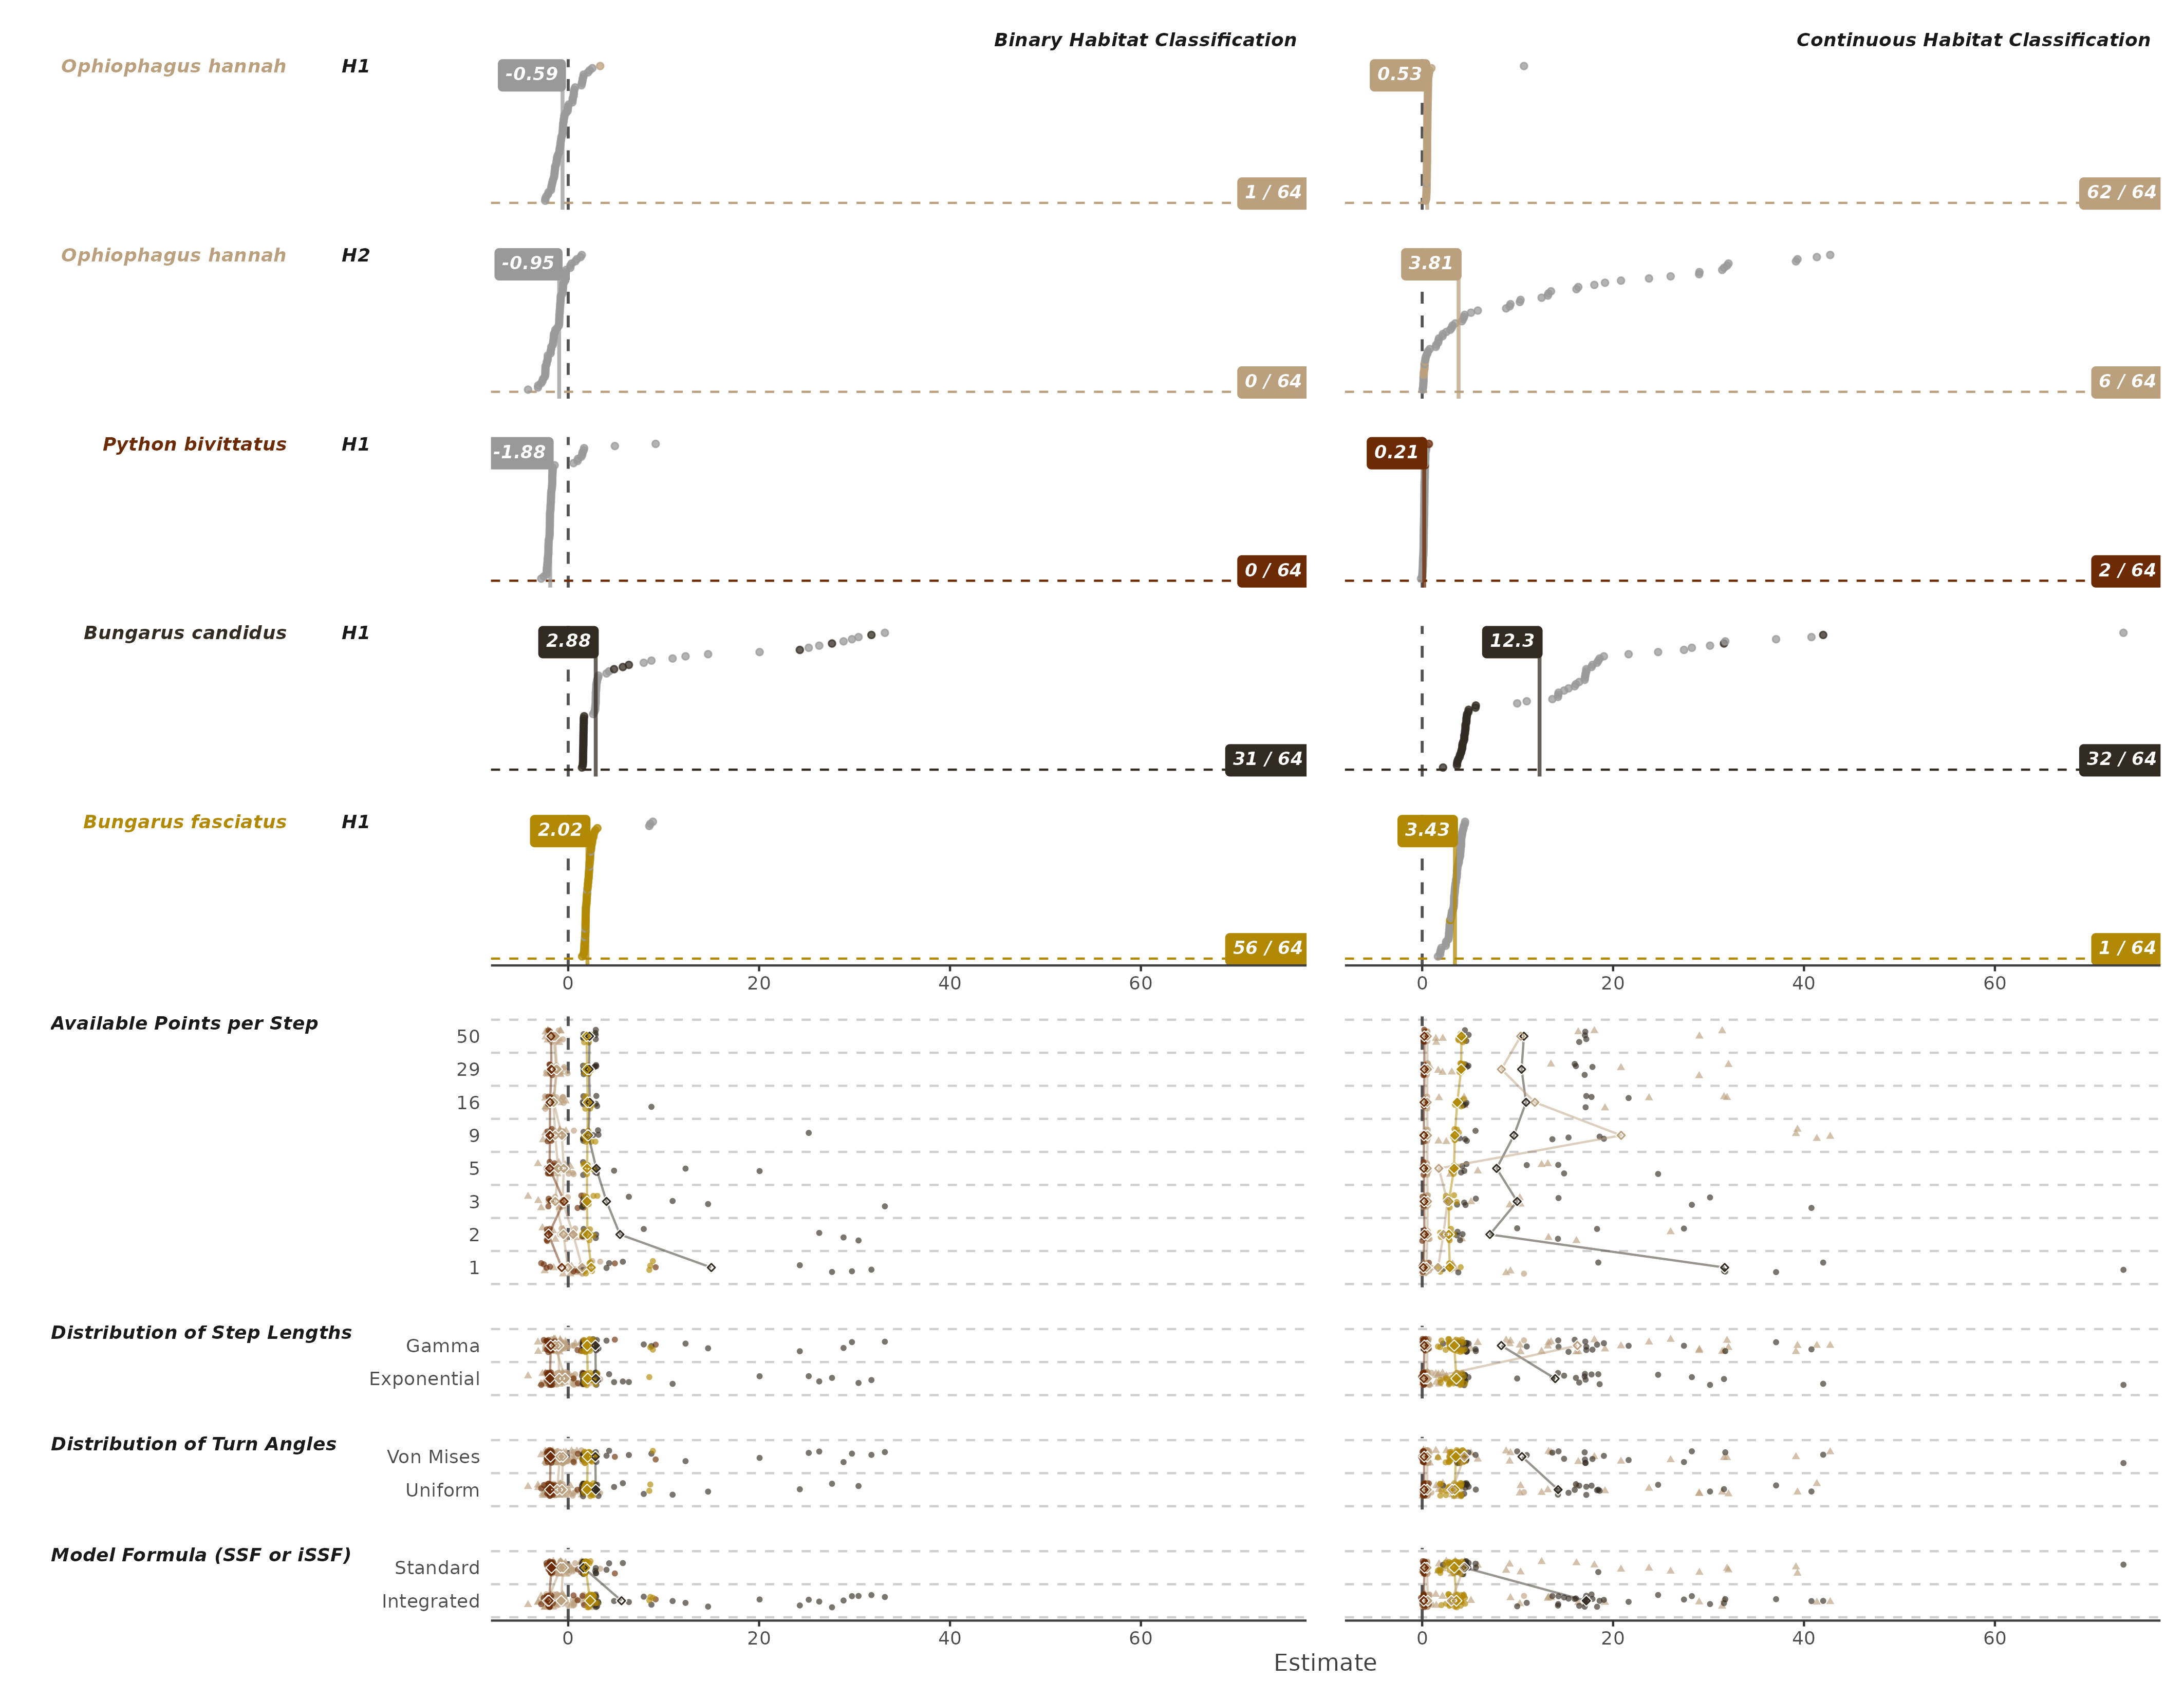
\includegraphics[width=1\linewidth]{../../figures/specCurve_ssf} \caption{All estimates of habitat selection derived from the step-based Step Selection Function (SSF) analysis. Top curves show all estimates, split by species and hypothesis, with coloured points indicating those with point estimates supporting the hypothesis (i.e., > 0). Labelled vertical lines show the median estimate for each species-hypothesis combination. Lower plot show the estimates relative to each analysis choice. The colours depict the species, and shape separate hypothesis 1 and 2 for the King Cobras (circles = hypothesis 1, triangle = hypothesis 2). Median estimates are shown with hollow diamonds, and species-hypothesis medians are connected with appropriated coloured lines. The plot is split left and right for the analysis using a binary classification (left), and continuous inverted distance (right).}\label{fig:specCurveSsf}
\end{figure}

The Poisson model approach appears similar to the SSF results, with universal support for the hypotheses when examining the median estimates (Fig. \ref{fig:specCurvePois}).
Once again the most marginal support was seen in \emph{Ophiophagus hannah} H2, where both classification methods result in low median estimates of preference.
The marginal medians seem to be largely due to a single decision: whether or not to run an integrated model formulation.
In this case the integrated models provide far more conservative estimates of selection, and for \emph{Ophiophagus hannah} H2 with binary classification fall below zero (Fig. \ref{fig:specCurvePoisOPHA}).
The impact of model formulation appears for all species, but the most dramatic impacts are seen when paired with binary habitat classification.
What is missed from the point estimates, and median summaries, is the massive uncertainty surrounding estimates when using the binary classification.
Zero estimates when using the binary habitat are significantly providing support.
This contrasts with the continuous habitat classification, where all species-hypothesis combinations show complete or majority significant support.
The impacts of other decisions are considerably smaller that model formulation.
There appears to be advantages to generating more available points, as estimates with few points tend to explain the upper and lower outliers.
The mitigation of extreme estimates is best seen in \emph{Bungarus fasciatus} when using a continuous habitat classification (Fig. \ref{fig:specCurvePoisBUFA}).

\begin{figure}
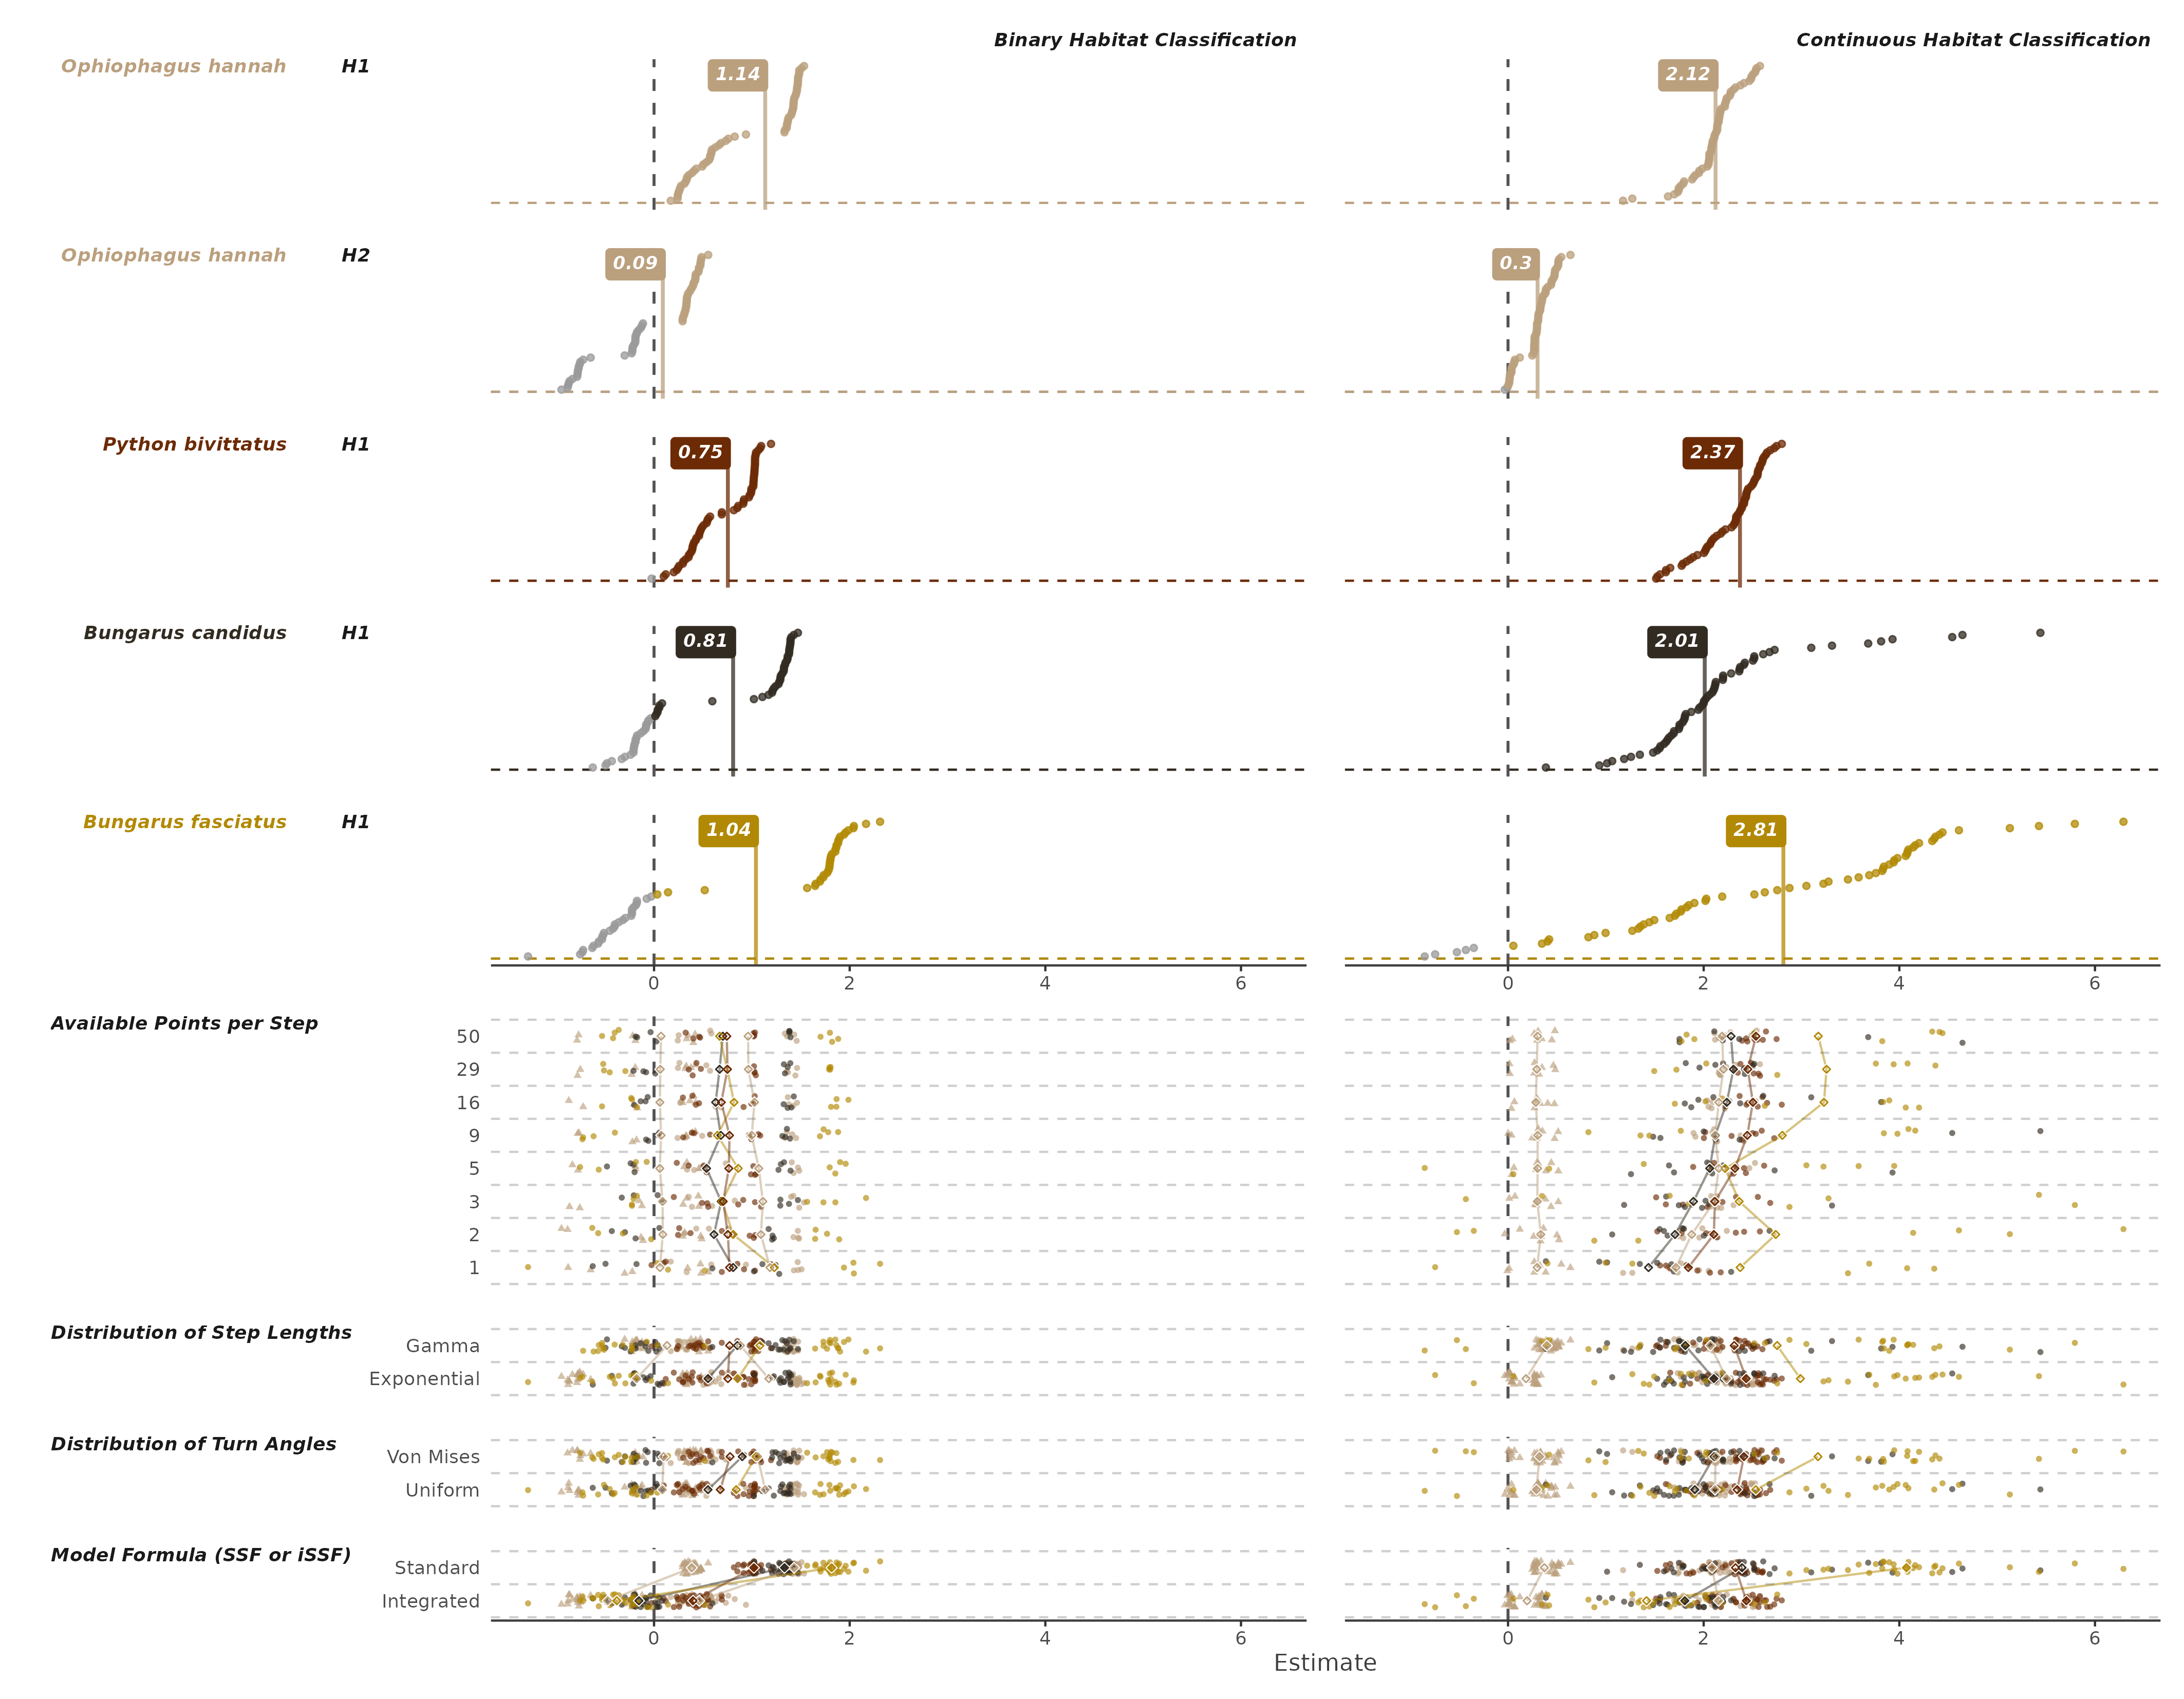
\includegraphics[width=1\linewidth]{../../figures/specCurve_pois} \caption{All estimates of habitat selection derived from the step-based Poisson model (Poisson) analysis. Top curves show all estimates, split by species and hypothesis, with coloured points indicating those with point estimates supporting the hypothesis (i.e., > 0). Labelled vertical lines show the median estimate for each species-hypothesis combination. Lower plot show the estimates relative to each analysis choice. The colours depict the species, and shape separate hypothesis 1 and 2 for the King Cobras (circles = hypothesis 1, triangle = hypothesis 2). Median estimates are shown with hollow diamonds, and species-hypothesis medians are connected with appropriated coloured lines. The plot is split left and right for the analysis using a binary classification (left), and continuous inverted distance (right).}\label{fig:specCurvePois}
\end{figure}

Our final analysis approach was using weighted Resource Selection Functions (wRSF).
All wRSF results provided support for the hypotheses (Fig. \ref{fig:specCurveWrsf}).
Although, once again, support for \emph{Ophiophagus hannah} H2 when using a continuous classification, is borderline and ultimately rounded to zero.
The strongest selection was seen in \emph{Ophiophagus hannah} H1, where both habitat classification methods unambiguously support the hypothesis.
All other species saw unambiguous support when the habitat was binary classed, but when classed continuously as inverted distance the 95\% confidence intervals for \emph{Python bivittatus} and \emph{Bungarus fasciatus} approximated zero.

\begin{figure}
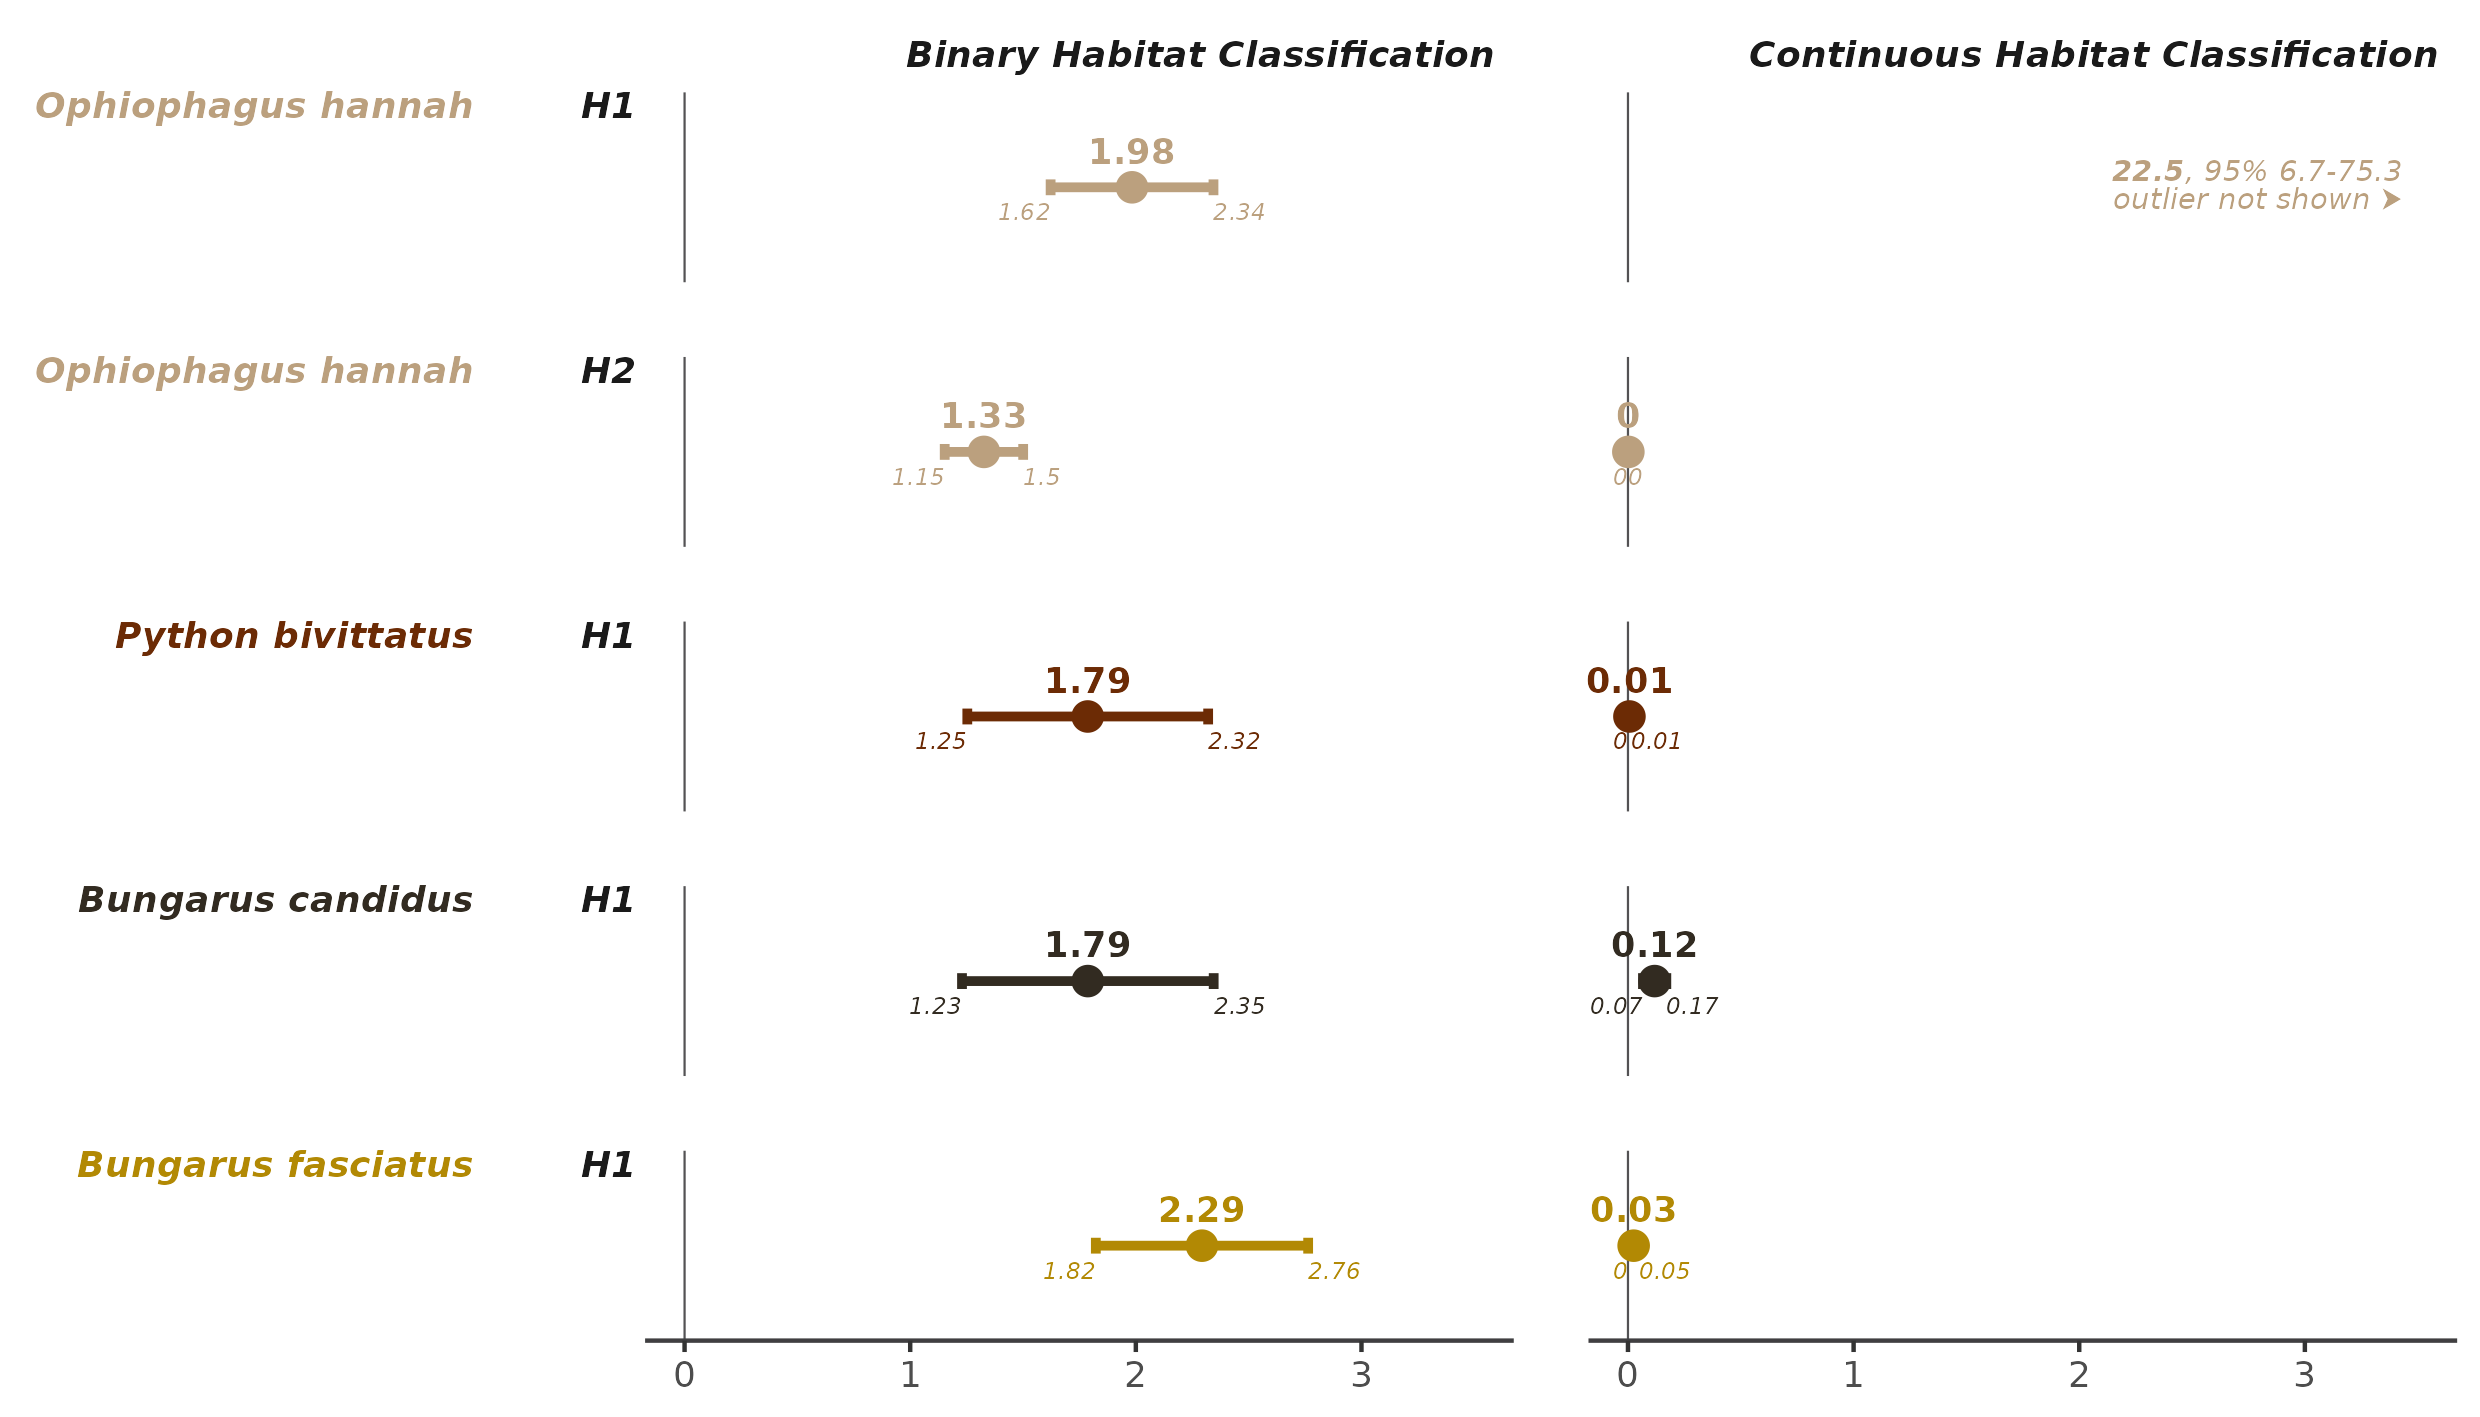
\includegraphics[width=1\linewidth]{../../figures/specCurve_wrsf} \caption{All estimates of habitat selection derived from the weighted Resource Selection Function (wRSF) analysis. Circles and numbers above show the point estimate, and the horizontal bar depict the 95\% confidence interval. The plot is split left and right for the analysis using a binary classification (left), and continuous inverted distance (right).The results for King Cobra (Ophiophagus hannah) H1 with the continuous habitat classification are hidden to aid with visualising all other estimates.}\label{fig:specCurveWrsf}
\end{figure}

\subsection{Meta-analysis Estimates}\label{meta-analysis-estimates}

The Bayesian meta-analyses tended to perform very well, with the population effects producing high \emph{R\textsuperscript{2}} values (22/45 \textgreater{} 0.6, median: 0.6 ±SD 0.31).
The RSF models had the highest \emph{R\textsuperscript{2}} values, with the continuous classification estimates being almost entirely described by the predictors (Fig. \ref{fig:metaR2Plot}).
The step-based approaches tended to have more variable \emph{R\textsuperscript{2}}, with step-selection models having the lowest values.

\emph{\(\tau\)\textsuperscript{2}} values ranged from very low (0.0061) for the binary classed RSF models examining \emph{Bungaurs facsiatus}, to 1.6 for the binary classed Poisson models examining the same species.
Mostly \emph{\(\tau\)\textsuperscript{2}} values below 0.1 27/45 (overall median of 0.05 ±SD 0.42), largely mirroring results gained from meta-analyses and ecological many analysts projects (\citeproc{ref-gould_same_2023}{Gould et al., 2023}).

\begin{figure}
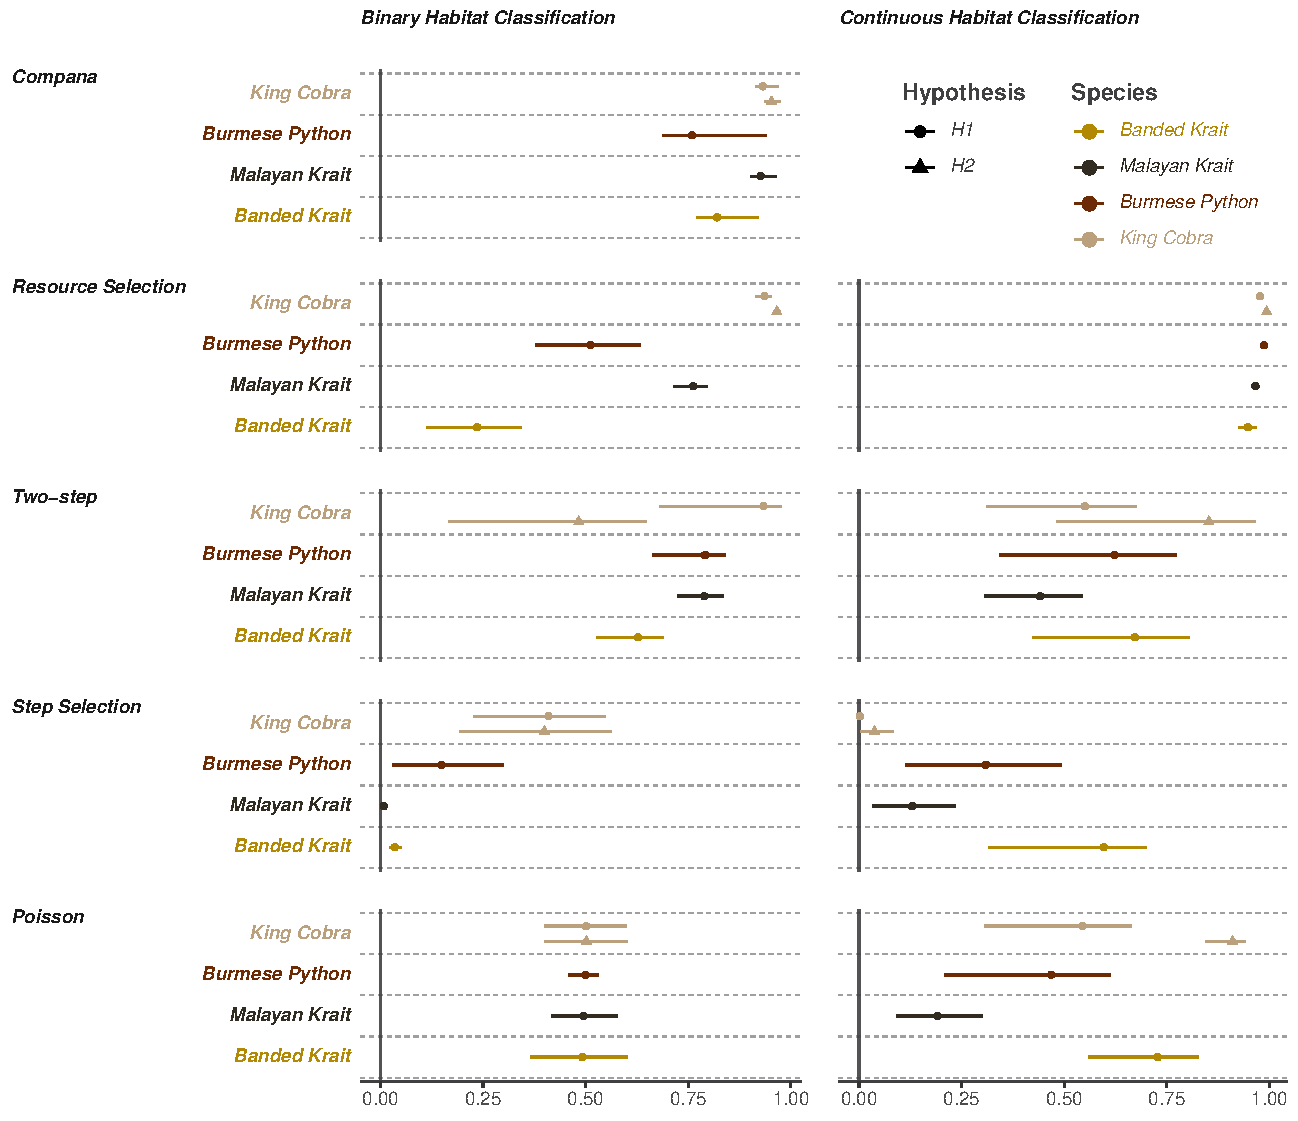
\includegraphics[width=1\linewidth]{../../figures/r2Plot} \caption{Conditional R2 values for all meta-analysis models, with 95\% HDCIs.}\label{fig:metaR2Plot}
\end{figure}

The intercepts of the meta-analyses models reveal that most hypothesis are overall supported, with the only exceptions existing when the habitat was binary classified (Fig. \ref{fig:metaInterPlot}).
\emph{Ophiophagus hannah} H2 and \emph{Python bivittatus} H1 using Compana, \emph{Bungarus candidus} H1 using Two-Step, \emph{Ophiophagus hannah} H2 and \emph{Python bivittatus} H1 using SSF.

\begin{figure}
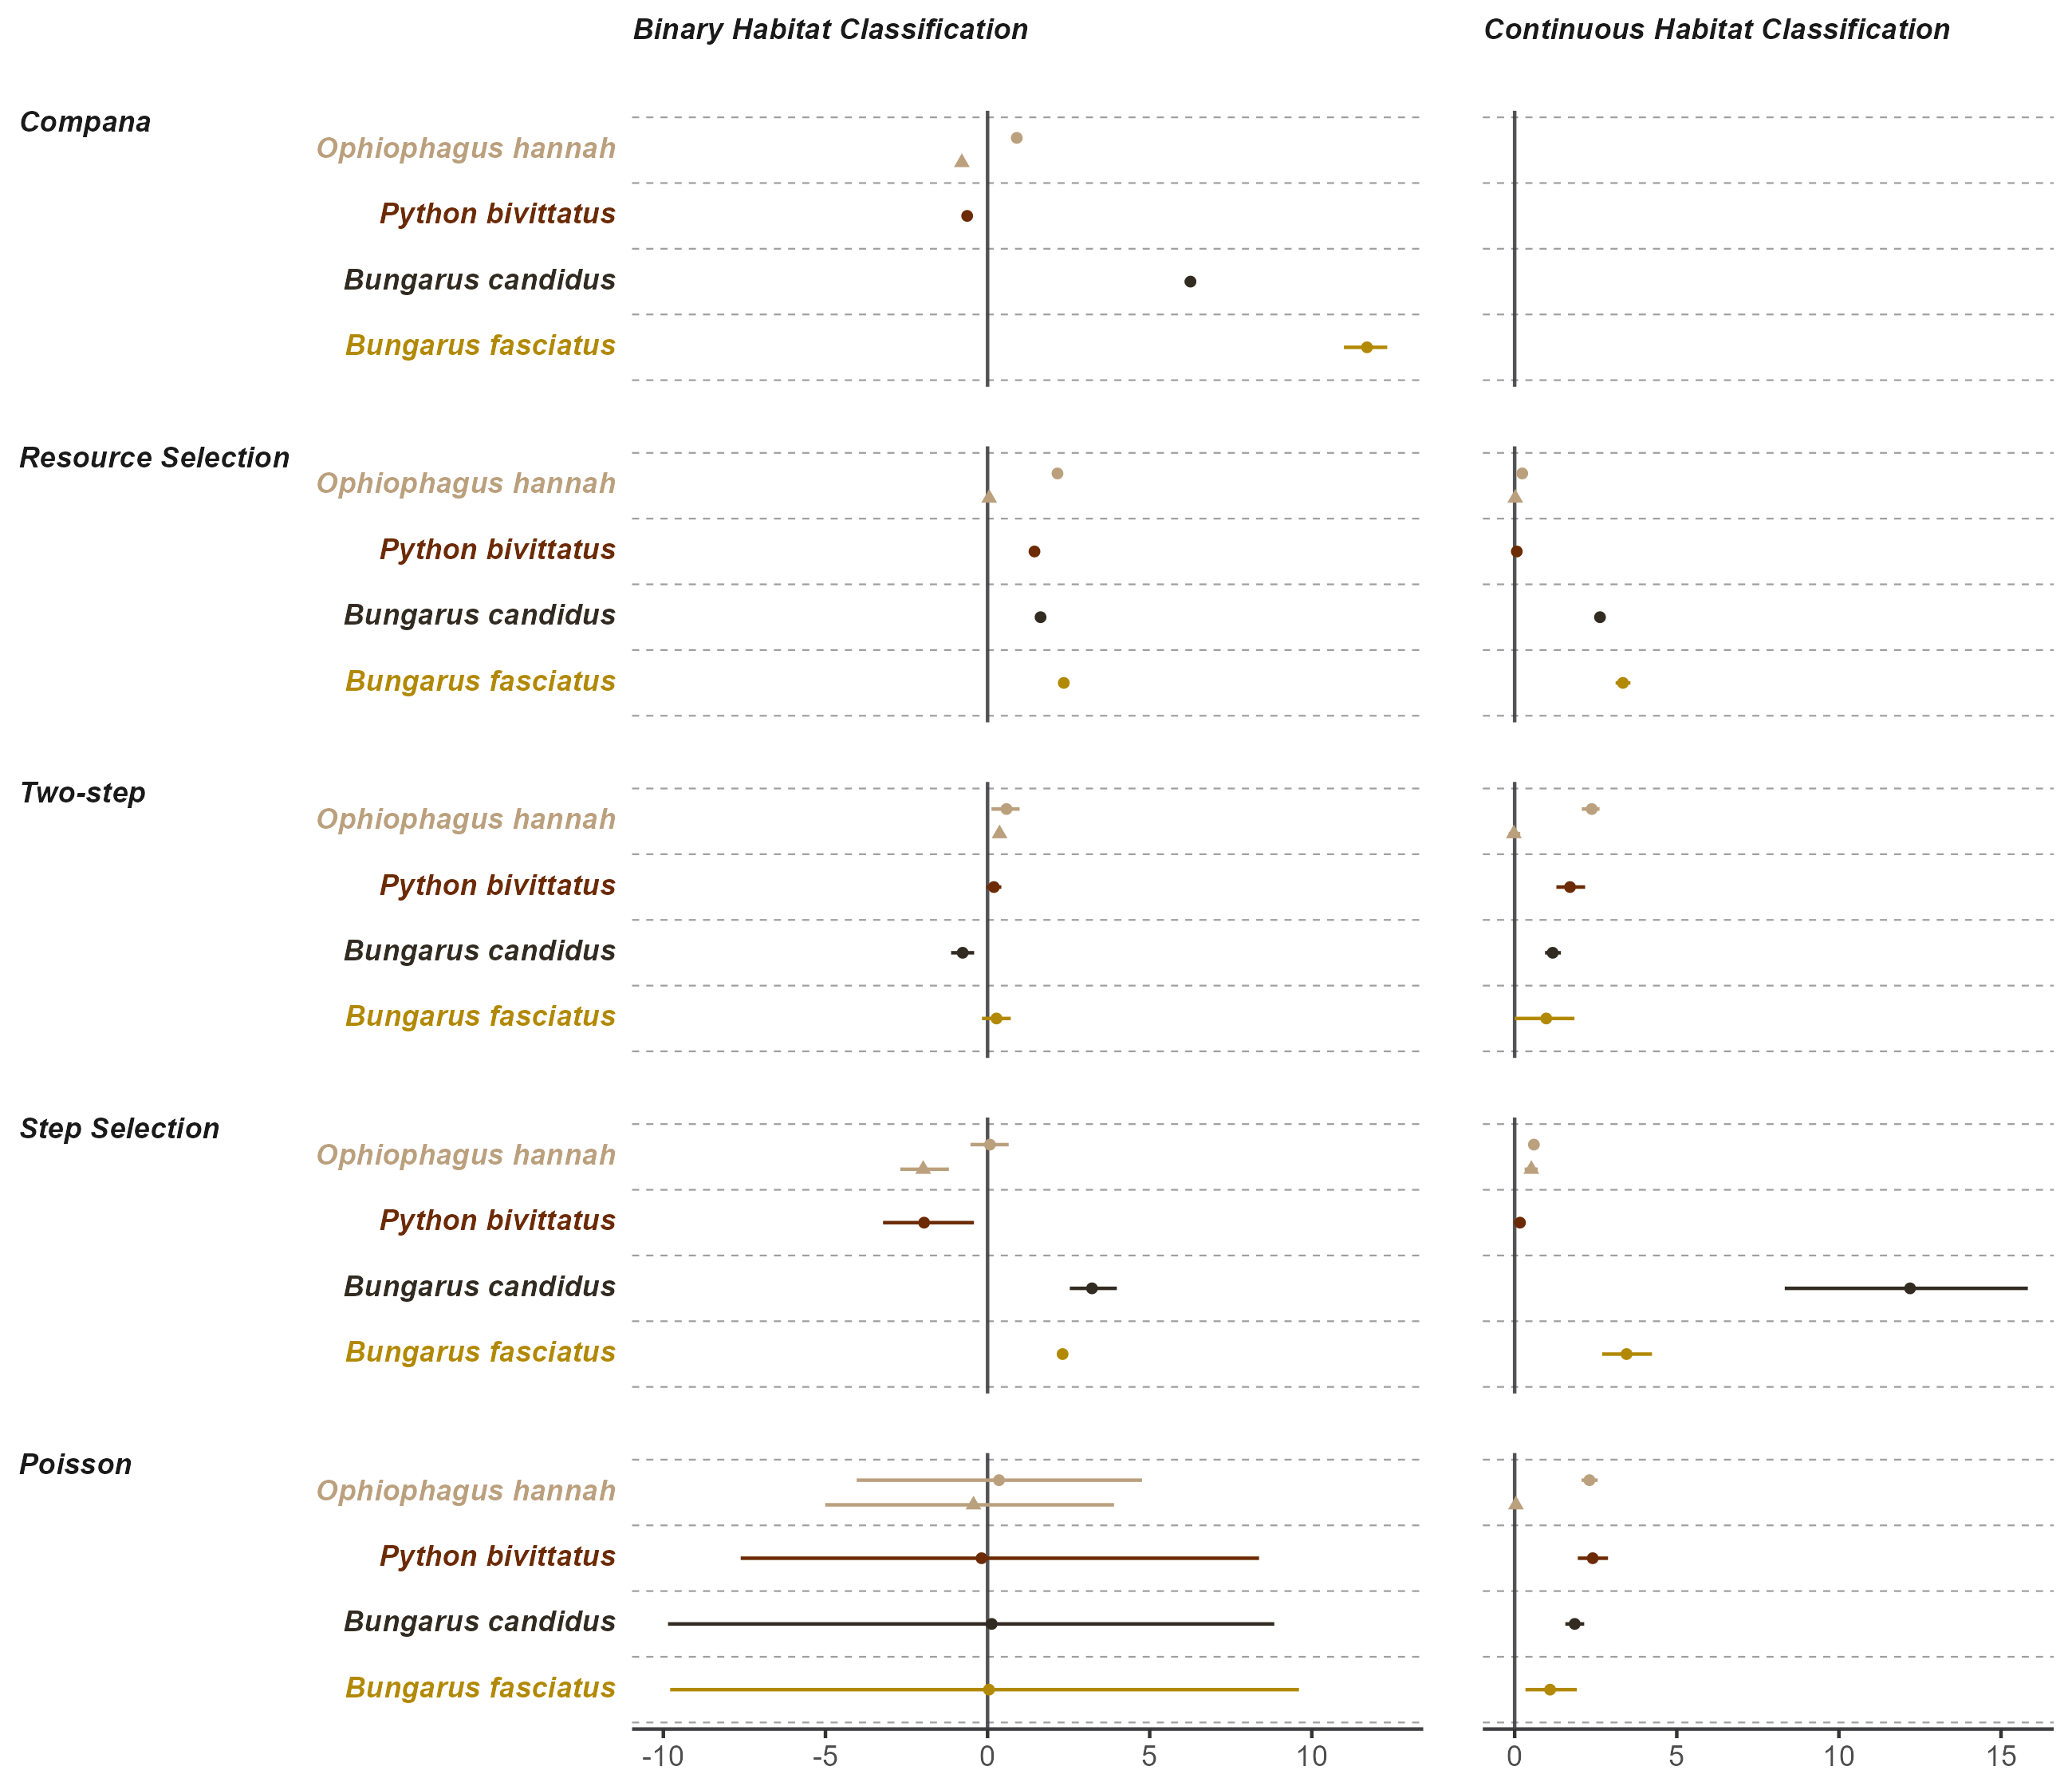
\includegraphics[width=1\linewidth]{../../figures/metaIntercept} \caption{Posterior estimates of the intercept for all meta-analysis models, with 95\% HDCIs.}\label{fig:metaInterPlot}
\end{figure}

Overall the patterns of meta-analysis results mirror the specification curves, and the similarities reappear in the analysis choice impacts.
Model formulation appeared as the most dramatic effect on the meta-analysis estimate, and that effect is seen in all three step-based approaches (Fig. \ref{fig:metaBetasPlot}).
The effects themselves were not consistent, with different directions and strengths depending on approach and species.
Only \emph{Bungarus fasciatus} was impacted consistently the same way, with the non-integrated estimates tending to have a positive impact on the estimates (Fig. \ref{fig:metaBetasPlot}).
Another choice that appears to have considerable impact was the available area method.
Like the model formulation, the impact varied by species and landscape classification.
It reveals that impact of available area method is not necessarily very predictable, and likely interacts with the specific movement characteristics of the study species.
Available points, either steps or points within an area, tended to be positively related to estimate strength.
This was reasonably universal, but the larger effects were seen in \emph{Bungarus spp.}, potentially suggesting greater impacts when the habitat's are defined at a finer spatial scale.

\begin{figure}
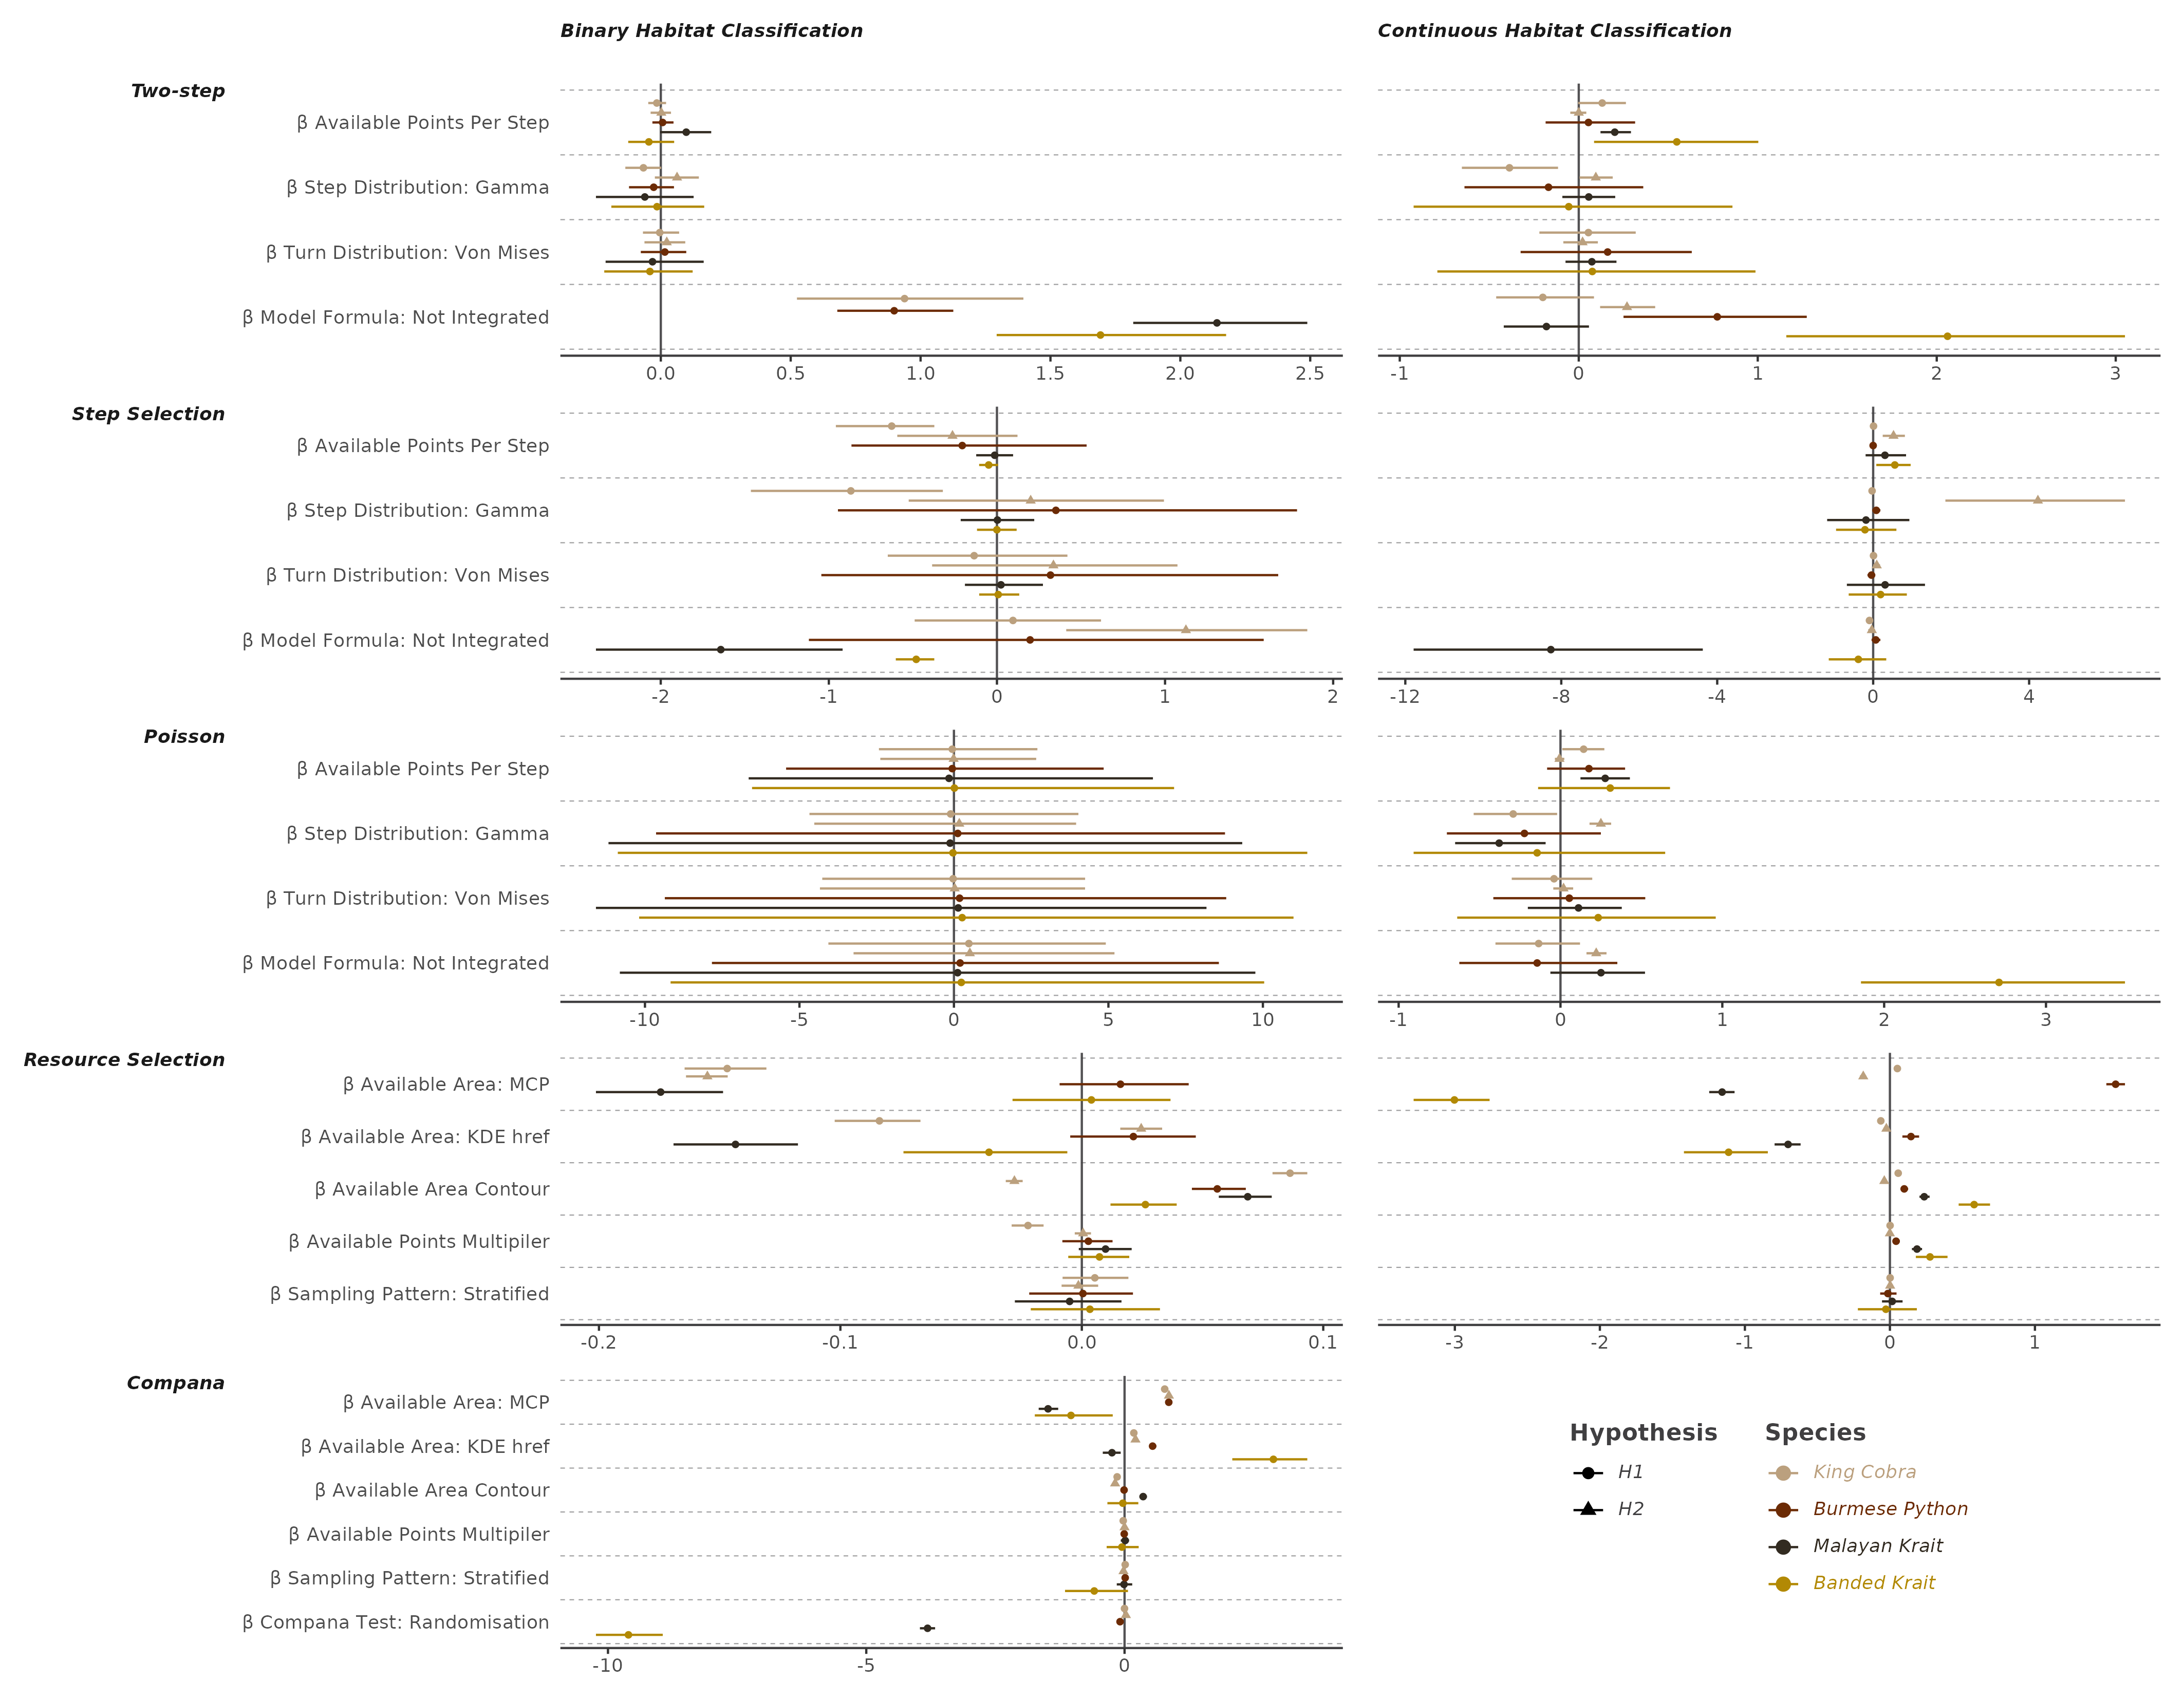
\includegraphics[width=1\linewidth]{../../figures/metaBeta} \caption{Posterior estimates of the population effects for all meta-analysis models, with 95\% HDCIs.}\label{fig:metaBetasPlot}
\end{figure}

\section{Discussion}\label{discussion}

Our re-testing of snake habitat selection studies using a multiverse of over 4915 analysis endpoints, suggests that the original conclusions remain broadly supported.
More specifically it appears that there is a reasonably low chance that the analysis choices made in the original publications led to strange or outlying results.
While the multiverse revealed broad support for the direction of the selection, the strength of the effect was more sensitive and we did identify a few analysis choices capable of contradicting the originally published results.

Of the four species we examined, \emph{Python bivitattus}'s preference for water bodies appears the most marginal, but the preference was clear in all bar six RSF analyses and the wRSF analysis.
All these analysis approaches have different assumptions, and treat the data in different ways.
Therefore, the apparent disagreement between RSF and other methods may tell us something about the preference that \emph{Python bivitattus} are demonstrating.
\emph{Python bivitattus} are ambush hunters; therefore, their movements may be less informative compared to their overall location in the landscape.
Particularly if they remain at the same location for extended periods, for example during nesting (\citeproc{ref-smith_risk_2024}{Smith et al., 2024}).
RSFs' de-emphasis of movement compared to step-based methods, may explain the differences in support.
The support from the more modern wRSF may also be ascribable to a broader selection for water bodies.

We only saw two decisions that could clearly alter conclusions, and even those did not appear universal.
\emph{Bungarus fasciatus} selection for field margins was supported by the vast majority of analyses, but the weakest support was when using Compositional analysis.
While the point estimates still suggested selection, a decision to use randomisation rather than parametric tests for significance would render all analysis non-significant.
Previous simulated scenarios have also revealed the sensitivity of estimates to this choice {[}chapter 3{]}.
Other species did not see the same impact; randomisation did lead to reduced strength estimates in \emph{Bungarus candidus}, but all remained significant.
We suspect the weaker support seen in Compositional Analysis may be the result of location error.
Compositional analysis could only be used with the binary habitat classification.
While every effort was made during tracking to ensure a correct GPS location was retrieved, error is unavoidable especially in denser forested areas or near buildings.
Even small errors may lead to mismatches between the true location (and habitat) of an animal and the land-use data we had access to.
This mismatch may be more pronounced when habitats are rarer or when animals tend to remain near its edges.
\emph{Bungarus fasciatus}'s focus on very thin field margins may have made it particularly susceptible, and similarly \emph{Python bivitattus}'s selection for the banks of water bodies.
The rarity of these habitats may have also played a role, as we see clear decrease in the confidence intervals surrounding the estimates as we increased the number of available points sampled.
We suspect that location error resulting in binary habitat mis-classification may explain the large confidence intervals of the Poisson models and the limited support in \emph{Python bivitattus} SSF analyses, as this uncertainty and lack of support is not visible in the continuous habitat models.

A second decision that could alter estimate strength dramatically was whether use an integrated model formulation (i.e., include step and turn angle in the model formula).
The work of (\citeproc{ref-muff_accounting_2020}{Muff, Signer \& Fieberg, 2020}) and (\citeproc{ref-forester_accounting_2009}{Forester, Im \& Rathouz, 2009}), as well as chapter 3 showed that integrated formulas have contrasting impacts on estimates in step-selection approaches and poisson models.
The step-selection models tend to produce less biased estimates when using an integrated formula, whereas the poisson models the opposite.
With those findings in mind, we should weight the findings using the non-integrated poisson models more heavily.
The non-integrated poison models show clearer support for the hypotheses in all cases with either classification, bar \emph{Ophiophagus hannah} H1 and \emph{Python bivitattus} H1 whose estimates seem negligibly impacted when using the continuous classification.
Unexpectedly the choice of model formulation did not have as noticeable impact in the step-selection approach, there only \emph{Bungarus candidus}'s estimates were markedly impacted.
Despite this, the strength of the selection exhibited by \emph{Bungarus candidus} meant that the more conservative estimates from the non-integrated models did not render the selection estimates non-significant.

Overall, we found that the final estimates could not be completely predicted by the analysis choices, despite there existing no sampling variation in the primary data.
In some cases, such as RSF binary, the analysis decisions explained the vast majority of variation and \emph{\(\tau\)\textsuperscript{2}} indicated that there was very little heterogeneity between end points.
Whereas others such as the Poisson binary meta-analysis models left most of the variation unexplained, and indicated much higher levels of between end point heterogeneity, which appear comparable to meta-analysis on multiple real studies that would also need to be contending with sampling variation.
The propensity for the step-based methods to show higher \emph{\(\tau\)\textsuperscript{2}} values could be due to random sampling of step and turn angles in the available points.
Overall, the variation in \emph{\(\tau\)\textsuperscript{2}} and \emph{R\textsuperscript{2}} values from the meta-analysis models indicate that analysis choices are interacting with the species data and hypothesis, suggesting variation in habitat selection estimates may be difficult to predict in other systems and limited the generalisably of patterns shown here.

Despite the clear species-driven variation in how analysis choices impact final estimates, we can examine the results on a species-hypothesis-basis to determine whether overall our multiverse supports or contradicts previously published conclusions.
While the average or summation or multiverse findings cannot be used as to estimate a true effect, they do highlight the high likelihood of repeated analyses agreeing.
Their agreement with the other results (in terms of direction), and the fact they largely provide significant support for the original hypothesis is reason to be confident in the original conclusions.

\subsection{Conlcusions}\label{conlcusions}

\subsubsection{\texorpdfstring{King Cobra \emph{Ophiohagus hannah}}{King Cobra Ophiohagus hannah}}\label{king-cobra-ophiohagus-hannah}

For \emph{Ophiophagus hannah} we examined two hypotheses.
The previously published conclusions that they make heavy use of semi-natural areas (i.e., banks of irrigation canals, and scrub between fields; Marshall et al. (\citeproc{ref-marshall_no_2020}{2020a})) is nearly universally supported regardless of approach, especially when classified as invert continuous distance.
Why \emph{Ophiophagus hannah} uses these habitats is not immediately clear, but it could be driven by prey availability (e.g., other snake species Barnes et al. (\citeproc{ref-Barnes2017}{2017}); Strine et al. (\citeproc{ref-Strine2018a}{2018})), the avoidance of threats, and density of shelter sites.
Other reptiles are know to make use of linear habitats (\citeproc{ref-Kay2016}{Kay et al., 2016}; \citeproc{ref-doherty_animal_2019}{Doherty, Fist \& Driscoll, 2019}), including other snakes at this study site (i.e., \emph{Ophiophagus hannah}'s primary prey; Jones et al. (\citeproc{ref-Jones_supposed_2020}{2020})).
Both prey and \emph{Ophiophagus hannah} could be using these linear connected semi-nat areas a means of avoiding the more exposed and dangerous fields and anthropogenic areas.
Human activity in fields, such as ploughing will kill snakes (\citeproc{ref-Knierim2017a}{Knierim, Barnes \& Hodges, 2017}), and we have documented many fatalities of \emph{Ophiophagus hannah} as a direct result of human actions (e.g., persecution, road collision; Marshall et al. (\citeproc{ref-marshall_no_2020}{2020a})).
We can be confident that suggestions regarding the importance of edge or scrub habitats amongst a human-modified landscape are robust in the face of a multitiude of analysis choices.

The second hypothesis regarding their selection for forest was not nearly as widely supported, and only appears to be supported in certain analysis approaches.
The original paper highlighted the propensity for \emph{Ophiophagus hannah} to leave the forest (\citeproc{ref-Marshall2018}{Marshall et al., 2019}), and the heightened movement particularly during breeding season, potentially mate searching behaviour.
Mate searching has been indicated as a potential seasonal driver of heightened movements in other snake species (\citeproc{ref-Duvall1997}{Duvall \& Schuett, 1997}; \citeproc{ref-Bauder2016a}{Bauder et al., 2016}).
The \emph{Ophiophagus hannah} data included in the first paper was more skewed towards \emph{Ophiophagus hannah} found in/near protected forest, hence the focus on forest use.
The data used here pooled old and new data that presents a more overall picture of \emph{Ophiophagus hannah} selection, likely weakened that associated with protected forest.
However, data collected after the original paper showed individuals using the forest for nesting; to maintain access to the forest these individuals travelled via semi-natural areas and were required to cross roads (\citeproc{ref-marshall_no_2020}{Marshall et al., 2020a}; \citeproc{ref-jones_how_2022}{Jones et al., 2022}).
The nest construction of \emph{Ophiophagus hannah} requires adequate vegetated material to maintain the requisite internal nest temperatures (\citeproc{ref-dolia_house-warming_2023}{Dolia, Das \& Kelkar, 2023}).
This highlights the potential importance of forested areas during certain times of year, even if it is less likely to be identified by the broad (rather generalised) habitat selection multiverse-analysis here.
Other studies have revealed \emph{Ophiophagus hannah} nesting potentially favours less disturbed areas, even if a clear preference of forests is not apparent (\citeproc{ref-koirala_distribution_2021}{Koirala \& Dawa Tshering, 2021}).

\subsubsection{\texorpdfstring{Burmese Python \emph{Python bivitattus}}{Burmese Python Python bivitattus}}\label{burmese-python-python-bivitattus}

The conclusions regarding \emph{Python bivitattus} habitat selection appear susceptible to differing analysis approaches, but overall we can be fairly confident that the assertion that \emph{Python bivitattus} ideally remain closer to water bodies.
The patterns of selection in \emph{Python bivitattus} appear more clearly with broader landscape level approaches compared to those using steps.
It is likely that \emph{Python bivitattus} are prioritising being close to water bodies for food and shelter.
The use of water bodies and aquatic landscapes is well documented in \emph{Python bivitattus}'s invasive range in Florida, USA (\citeproc{ref-mutascio_modeling_2018}{Mutascio et al., 2018}); and here in Thailand evidence of \emph{Python bivitattus} capitalising on both shelter and prey provided by the water bodies is apparent.
As mentioned for the \emph{Ophiophagus hannah}, edge areas in agricultural land in this area of Thailand are considerably less trafficked and modified compared to the agricultural matrix of crops.
Less disturbance likely boosts shelter site options, as well as ambush sites and associated prey (e.g., aquatic birds).
Shelter sites along edge habitats, such as field margins and banks, appear to shelter suitable for nesting (also evidenced by \emph{Bungarus fasciatus} nest site choice; Smith et al. (\citeproc{ref-smith_risk_2024}{2024})).
Nesting requires prolonged periods of non-disturbance, evidencing the potential stability of some of these edge habitat areas.
Whereas for food, rice paddies can house suitable sized water birds (\citeproc{ref-fujioka_bird_2010}{Fujioka, Don Lee \& Kurechi, 2010}), and \emph{Python bivitattus} in this area have been documented depredating domestic waterfowl (\citeproc{ref-smith_native_2021}{Smith et al., 2021}), together supporting suggestions that the water bodies are a resource.

\subsubsection{\texorpdfstring{Malayan Krait \emph{Bungarus candidus}}{Malayan Krait Bungarus candidus}}\label{malayan-krait-bungarus-candidus}

The previously published conclusions that \emph{Bungarus candidus} prefer buildings and natural areas appears to be the most clearly supported and one of the least susceptible to analysis choices.
Broadly the analysis would support their selection for buildings and natural areas on the university campus.
We suspect the support is not due to a particular movement pattern, but instead the strength of the selection, which is visible in the wRSF and meta-analysis intercepts.
\emph{Bungarus candidus} are likely avoiding open areas, instead choosing to make use of the better micro-habitats available in buildings and natural areas.
Hodges et al. (\citeproc{ref-hodges_malayan_2022}{2022}) suggests these environments may be better for thermoregulation, and other evidence reveals buildings are used for foraging (\citeproc{ref-hodges_diurnal_2020}{Hodges, D'souza \& Jintapirom, 2020}; \citeproc{ref-hodges_deadly_2021}{Hodges et al., 2021a}).
The selection for buildings presents a clear potential for human-snake conflict.
\emph{Bungarus candidus} are highly medically significant (\citeproc{ref-looareesuwan_factors_1988}{Looareesuwan, Viravan \& Warrell, 1988}; \citeproc{ref-searo_regional_office_for_the_south_east_asia_rgo_guidelines_2016}{South East Asia (RGO) \& Asia, 2016}), and apparent overlap between their preference and human movements could heighten the chances of human-snake interactions resulting the harm of either human or snake.
Fortunately, \emph{Bungarus candidus} are mostly nocturnal presenting the chance for human and snake to avoid conflict temporally.
The robustness of the selection analyses means we can safely support the suggestions in Hodges et al. (\citeproc{ref-hodges_malayan_2022}{2022}) for the university to encourage light use when moving in the evening and night, wearing of closed footwear, and ensure buildings are adequately sealed (\citeproc{ref-samuel_venomous_2020}{Samuel et al., 2020}).
The selection for natural areas may further present an opportunity to draw snakes away from buildings, if more ideal shelter sites are available farther from concentrations of human activity.
Studies elsewhere in Thailand have suggested that other medically significant snakes will avoid buildings, preferring more vegetated areas (\citeproc{ref-barnes_snake_2024}{Barnes et al., 2024}).

\subsubsection{\texorpdfstring{Banded Krait \emph{Bungarus fasciatus}}{Banded Krait Bungarus fasciatus}}\label{banded-krait-bungarus-fasciatus}

\emph{Bungarus fasciatus} conclusions fall mostly in the middle, they are very well supported by the overall meta-analysis intercepts but did clearly reveal some scenarios where researcher choice could have obscured what appears to be a selection for field margins.
As mentioned for \emph{Ophiophagus hannah}, field margins and other edge habitats, appear key to snake's lives in agricultural areas in Northeast Thailand, providing shelter and movement corridors.
\emph{Bungarus fasciatus} supports this.
Their use of edge habitats is not limited to sheltering, as like \emph{Python bivitattus}, the edges offer suitable (possibly communal) nest sites (\citeproc{ref-knierim_spatial_2019}{Knierim, 2019}).
When paired with other studies indicating the importance of field margins for mammalian and amphibians (\citeproc{ref-brown_habitat_2001}{Brown \& Singleton, 2001}; \citeproc{ref-groffen_preference_2018}{Groffen, Borzée \& Jang, 2018}), particularly rice paddy edges, it is clear that \emph{Bungarus fasciatus} likely finds all the resources required in these edge habitats.
The concentration to the field margins may indicate a human-snake interaction hotspot, the identification of which could aid refinement of agent-based snakebite risk maps (e.g., Goldstein et al. (\citeproc{ref-goldstein_integrating_2021}{2021})).

Looking forward, we feel confident in the broad conclusions draw by the original studies and that the analyses choices of the original publications did not result in peculiarly conclusions.
The support originating from more modern methods is additionally reassuring.
The wRSFs should be best placed to provide us with a broad estimate of habitat selection, while also best positioned to tackle the issues arising from inconsistent tracking (\citeproc{ref-alston_mitigating_2023}{Alston et al., 2023}).
However, the use of exact selection strengths should be examined in more detail if they are to be adapted to future purposes such as human-snake conflict prediction (as supported by simulation habitat multiverses; Marshall \& Duthie (\citeproc{ref-marshall_habitat_2024}{2024}); Chapter 3).
In those cases reassessment of the selection using newer methods more acutely tailored to prediction may be required, either by greater integration of mechanistic drivers of snake movement, or via methods that are scale independent enabling better beyond-sample extrapolation (e.g., Michelot et al. (\citeproc{ref-michelot_langevin_2019}{2019})).

Summarised together, this study reveals the robustness of snake habitat selection studies to researcher analysis choice, while also reaffirming the conclusions regarding the important role habitat patches (edges, banks, canals, etc.) play for snakes in an otherwise human dominated unsuitable landscape.

\section{Acknowledgements}\label{acknowledgements}

BMM was funded by the Natural Environment Research Council (NERC) via the IAPETUS2 Doctoral Training Partnership.

\section{Software availablity}\label{software-availablity}

All code used in the creation of this manuscript is available at \ldots{}

In addition to packages already mentioned in the methods we also used the following.

We used \emph{R} v.4.2.2 (\citeproc{ref-base}{R Core Team, 2022}) via \emph{RStudio} v.2023.6.2.561 (\citeproc{ref-rstudio}{RStudio Team, 2022}).
We used \emph{here} v.1.0.1 (\citeproc{ref-here}{Müller, 2020}), \emph{readr} v.2.1.5 (\citeproc{ref-readr}{Wickham, Hester \& Bryan, 2024}), \emph{inborutils} v.0.3.0 (\citeproc{ref-inborutils}{Van Calster, Oldoni \& Van Hoey, 2023}), and \emph{qs} v.0.26.3 (\citeproc{ref-qs}{Ching, 2023}) to manage directory addresses and saved objects.

We used \emph{ggplot2} v.3.5.1 for creating figures (\citeproc{ref-ggplot2}{Wickham, 2016}), with the expansions: \emph{patchwork} v.1.2.0 (\citeproc{ref-patchwork}{Pedersen, 2024}), \emph{ggridges} v.0.5.6 (\citeproc{ref-ggridges}{Wilke, 2024}), \emph{ggtext} v.0.1.2 (\citeproc{ref-ggtext}{Wilke \& Wiernik, 2022}), \emph{ggnewscale} v.0.5.0 (\citeproc{ref-ggnewscale}{Campitelli, 2024}), and \emph{ggdist} v.3.3.2 (\citeproc{ref-ggdist}{Kay, 2023a}).

We used \emph{brms} v.2.21.0 (\citeproc{ref-brms}{Bürkner, 2021}) to run Bayesian models, with diagnostics generated used \emph{bayesplot} v.1.11.1 (\citeproc{ref-bayesplot}{Gabry \& Mahr, 2024}), \emph{tidybayes} v.3.0.6 (\citeproc{ref-tidybayes}{Kay, 2023b}), and \emph{performance} v.0.11.0 (\citeproc{ref-performance}{Lüdecke et al., 2021}).

We used the \emph{dplyr} v.1.1.4 (\citeproc{ref-dplyr}{Wickham et al., 2023}), \emph{tidyr} v.1.3.1 (\citeproc{ref-tidyr}{Wickham, Vaughan \& Girlich, 2023}), \emph{tibble} v.3.2.1 (\citeproc{ref-tibble}{Müller \& Wickham, 2023}), and \emph{stringr} v.1.5.1 (\citeproc{ref-stringr}{Wickham, 2022}) packages for data manipulation.

We used \emph{sp} v.2.1.4 (\citeproc{ref-sp}{Pebesma \& Bivand, 2005}), \emph{sf} v.1.0.16 (\citeproc{ref-sf2018}{Pebesma, 2018}; \citeproc{ref-sfheaders}{Cooley, 2023}; \citeproc{ref-sf2023}{Pebesma \& Bivand, 2023}), \emph{raster} v.3.6.26 (\citeproc{ref-raster}{Hijmans, 2023a}), \emph{terra} v.1.7.78 (\citeproc{ref-terra}{Hijmans, 2023b}), \emph{tidyterra} v.0.6.0 (\citeproc{ref-tidyterra}{Hernangómez, 2023}), and \emph{move} v.4.2.4 (\citeproc{ref-move}{Kranstauber, Smolla \& Scharf, 2023}) for manipulation of spatial data and estimation of space use not otherwise mentioned in the methods.
We used \emph{ctmm} v.1.2.0 (\citeproc{ref-ctmm}{Fleming \& Calabrese, 2023}), \emph{amt} v.0.2.2.0 (\citeproc{ref-amt}{Signer, Fieberg \& Avgar, 2019}), \emph{adehabitatHS} v.0.3.17 (\citeproc{ref-adehabitatHS}{Calenge \& Mathieu Basille, 2023}), \emph{adehabitatHR} v.0.4.21 (\citeproc{ref-adehabitatHR}{Calenge \& Scott Fortmann-Roe, 2023}), \emph{lme4} v.1.1.35.3 (\citeproc{ref-lme4}{Bates et al., 2015}), \emph{INLA} v.23.4.24 (\citeproc{ref-INLA2}{Martins et al., 2013}; \citeproc{ref-INLA}{Lindgren \& Rue, 2015}), and \emph{TwoStepCLogit} v.1.2.5 (\citeproc{ref-TwoStepCLogit}{Craiu et al., 2016}) for the habitat analyses.

We used rmarkdown v.2.27 (\citeproc{ref-rmarkdown2018}{Xie, Allaire \& Grolemund, 2018}; \citeproc{ref-rmarkdown2020}{Xie, Dervieux \& Riederer, 2020}; \citeproc{ref-rmarkdown2023}{Allaire et al., 2023}), bookdown v.0.39 (\citeproc{ref-bookdown2016}{Xie, 2016}, \citeproc{ref-R-bookdown}{2022}), tinytex v.0.51 (\citeproc{ref-tinytex2019}{Xie, 2019}, \citeproc{ref-tinytex2023}{2023a}), and knitr v.1.47 (\citeproc{ref-knitr2014}{Xie, 2014}, \citeproc{ref-knitr2015}{2015}, \citeproc{ref-knitr2023}{2023b}) packages to generate type-set outputs.

We generated R package citations with the aid of \emph{grateful} v.0.2.4 (\citeproc{ref-grateful}{Francisco Rodríguez-Sánchez, Connor P. Jackson \& Shaurita D. Hutchins, 2023}).

\section{Data availabilty}\label{data-availabilty}

The majority of the data is already publicly available.
Movement data can be accessed via Movebank (\citeproc{ref-kays_movebank_2022}{Kays et al., 2022}), with the following study IDs: 1649411628, 556564170, 1093796277, 1204811528.
Movement data and land use data was also available via the following data repositories: Marshall et al. (\citeproc{ref-marshall_data_2020}{2020b}); Smith et al. (\citeproc{ref-smith_dataset_2020}{2020}); Hodges et al. (\citeproc{ref-hodges_malayan_2021}{2021b}).

For the ease of recreating the results presented here, we have uploaded all movement and land use data, alongside the code used to generate this manuscript.
If using this compiled data, we highly suggest also citing the original data paper and repository as listed above to ensure the data maintains a close connection to descriptions of its collection.

\section{Supplementary Material}\label{supplementary-material}

\subsection{Tracking Summary}\label{tracking-summary-1}

\begin{table}
\centering
\caption{\label{tab:trackingSummaryTable}Summary of tracking effort, tracking time lags (hours), and step lengths (metres) or each species.}
\centering
\resizebox{\ifdim\width>\linewidth\linewidth\else\width\fi}{!}{
\fontsize{8}{10}\selectfont
\begin{tabular}[t]{lcclccl}

Species & Individual ID & Number of Datapoints & Total Tracking Duration (days) & Mean Time Lag ± Standard Error (hours) & Number of Moves & Mean Step Length ± Standard Error (metres)\\
\hline
Bungarus candidus & BUCA001 & 116 & 107.50069 & 22.43 ±2.26 & 34 & 31.01 ±8.24\\
Bungarus candidus & BUCA002 & 230 & 222.77083 & 23.35 ±1.04 & 64 & 22.05 ±3.89\\
Bungarus candidus & BUCA007 & 130 & 144.47917 & 26.88 ±2.56 & 25 & 23.74 ±6.25\\
Bungarus candidus & BUCA012 & 144 & 161.97569 & 27.18 ±2.8 & 25 & 26.08 ±8.4\\
Bungarus candidus & BUCA014 & 77 & 80.65764 & 25.47 ±1.49 & 19 & 22.06 ±6.25\\
Bungarus candidus & BUCA016 & 112 & 116.19444 & 25.12 ±1.59 & 17 & 6.14 ±1.94\\
Bungarus candidus & BUCA022 & 51 & 56.67708 & 27.2 ±3.25 & 37 & 37.7 ±9.43\\
Bungarus candidus & BUCA027 & 32 & 36.78819 & 28.48 ±4.52 & 9 & 20.23 ±9.37\\
Bungarus candidus & BUCA028 & 117 & 106.53472 & 22.04 ±1.21 & 43 & 17.87 ±3.82\\
Bungarus candidus & BUCA032 & 99 & 107.65764 & 26.37 ±1.77 & 27 & 61.47 ±17.3\\
Bungarus candidus & BUCA033 & 179 & 187.49167 & 25.28 ±1 & 34 & 15.86 ±3.14\\
Bungarus candidus & BUCA035 & 141 & 144.82639 & 24.83 ±0.82 & 19 & 20.22 ±5.08\\
Bungarus candidus & BUCA036 & 54 & 68.72083 & 31.12 ±5 & 18 & 55.67 ±17.75\\
Bungarus fasciatus & BUFA001 & 475 & 829.00000 & 41.97 ±3.43 & 163 & 102.75 ±9.88\\
Bungarus fasciatus & BUFA003 & 217 & 260.00000 & 28.89 ±1.12 & 50 & 26.74 ±4.95\\
Bungarus fasciatus & BUFA004 & 182 & 212.00000 & 28.11 ±1.2 & 47 & 33.71 ±5.58\\
Ophiophagus hannah & OPHA002 & 667 & 223.75116 & 8.06 ±0.7 & 359 & 476.65 ±44.41\\
Ophiophagus hannah & OPHA004 & 122 & 46.74653 & 9.27 ±0.81 & 94 & 665.03 ±103.34\\
Ophiophagus hannah & OPHA005 & 664 & 180.68454 & 6.54 ±0.29 & 305 & 406.57 ±40.48\\
Ophiophagus hannah & OPHA006 & 2173 & 723.05397 & 7.99 ±0.17 & 553 & 71.88 ±4.23\\
Ophiophagus hannah & OPHA007 & 969 & 320.66087 & 7.95 ±0.29 & 225 & 72.24 ±6.71\\
Ophiophagus hannah & OPHA010 & 432 & 430.01319 & 23.95 ±15.56 & 83 & 52.16 ±10.75\\
Ophiophagus hannah & OPHA013 & 1497 & 561.19097 & 9 ±0.17 & 390 & 48.35 ±3.31\\
Ophiophagus hannah & OPHA014 & 247 & 67.83958 & 6.62 ±0.24 & 48 & 20.77 ±3.68\\
Ophiophagus hannah & OPHA015 & 1944 & 680.12986 & 8.4 ±0.18 & 595 & 71.05 ±4.74\\
Ophiophagus hannah & OPHA017 & 2245 & 774.96944 & 8.29 ±0.11 & 747 & 31.84 ±1.96\\
Ophiophagus hannah & OPHA018 & 3122 & 1176.09583 & 9.04 ±0.28 & 1018 & 75.72 ±4.06\\
Ophiophagus hannah & OPHA019 & 890 & 311.79028 & 8.42 ±0.21 & 231 & 43.22 ±4.97\\
Ophiophagus hannah & OPHA024 & 466 & 173.17292 & 8.94 ±0.27 & 217 & 100.56 ±9.13\\
Ophiophagus hannah & OPHA025 & 435 & 164.98403 & 9.12 ±0.36 & 203 & 69.62 ±7.79\\
Ophiophagus hannah & OPHA026 & 134 & 68.72847 & 12.4 ±0.72 & 68 & 107.46 ±20.53\\
Ophiophagus hannah & OPHA027 & 542 & 198.62500 & 8.81 ±0.23 & 126 & 22.96 ±2.98\\
Ophiophagus hannah & OPHA034 & 317 & 124.02222 & 9.42 ±0.42 & 52 & 37.75 ±7.35\\
Ophiophagus hannah & OPHA054 & 1381 & 520.62361 & 9.05 ±0.16 & 383 & 57.41 ±5.34\\
Ophiophagus hannah & OPHA055 & 722 & 353.61944 & 11.77 ±0.4 & 247 & 73.12 ±6.93\\
Ophiophagus hannah & OPHA056 & 428 & 162.07222 & 9.11 ±0.28 & 140 & 48.96 ±5.6\\
Ophiophagus hannah & OPHA058 & 672 & 268.89514 & 9.62 ±0.25 & 254 & 53.71 ±5.58\\
Ophiophagus hannah & OPHA059 & 995 & 345.03819 & 8.33 ±0.17 & 213 & 39.42 ±4.28\\
Ophiophagus hannah & OPHA086 & 623 & 241.01528 & 9.3 ±0.28 & 196 & 46.65 ±4.59\\
Ophiophagus hannah & OPHA096 & 291 & 132.91667 & 11 ±0.41 & 55 & 50.99 ±8.88\\
Ophiophagus hannah & OPHA099 & 276 & 122.01528 & 10.65 ±0.37 & 30 & 46.22 ±13.52\\
Python bivittatus & PYBI021 & 631 & 662.03125 & 25.22 ±0.33 & 216 & 31.79 ±3.05\\
Python bivittatus & PYBI022 & 438 & 485.89722 & 26.69 ±1.11 & 154 & 29.44 ±2.98\\
Python bivittatus & PYBI028 & 176 & 187.80417 & 25.76 ±0.78 & 69 & 70.05 ±12.29\\
Python bivittatus & PYBI029 & 486 & 514.91667 & 25.48 ±0.83 & 237 & 56.23 ±4.89\\
Python bivittatus & PYBI033 & 41 & 41.07639 & 24.65 ±0.6 & 22 & 36.38 ±7.88\\
Python bivittatus & PYBI055 & 205 & 207.12639 & 24.37 ±0.33 & 26 & 15.67 ±5.23\\
Python bivittatus & PYBI060 & 191 & 190.93819 & 24.12 ±0.25 & 63 & 65.09 ±9.91\\

\end{tabular}}
\end{table}

\begin{figure}
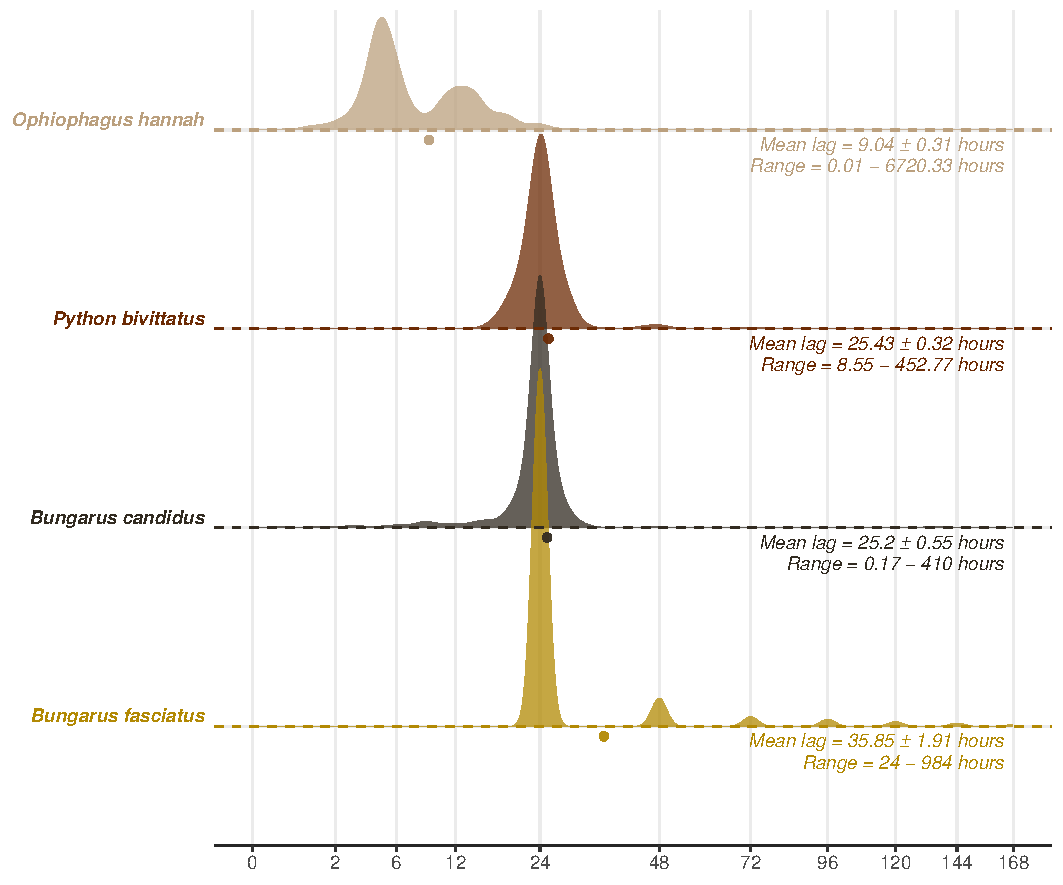
\includegraphics[width=1\linewidth]{../../figures/timeLagPlot} \caption{The distribution between subsequent data points for each species. Circles below the distributions show the media time lag. Reported alongside is the mean, standard error (±), and range of time lags. Large time lags are usually the result of prolonged missing periods or transmitter failures. N.b., the x axis is square-rooted to aid with visualisation.}\label{fig:timeLagPlot}
\end{figure}

\begin{figure}
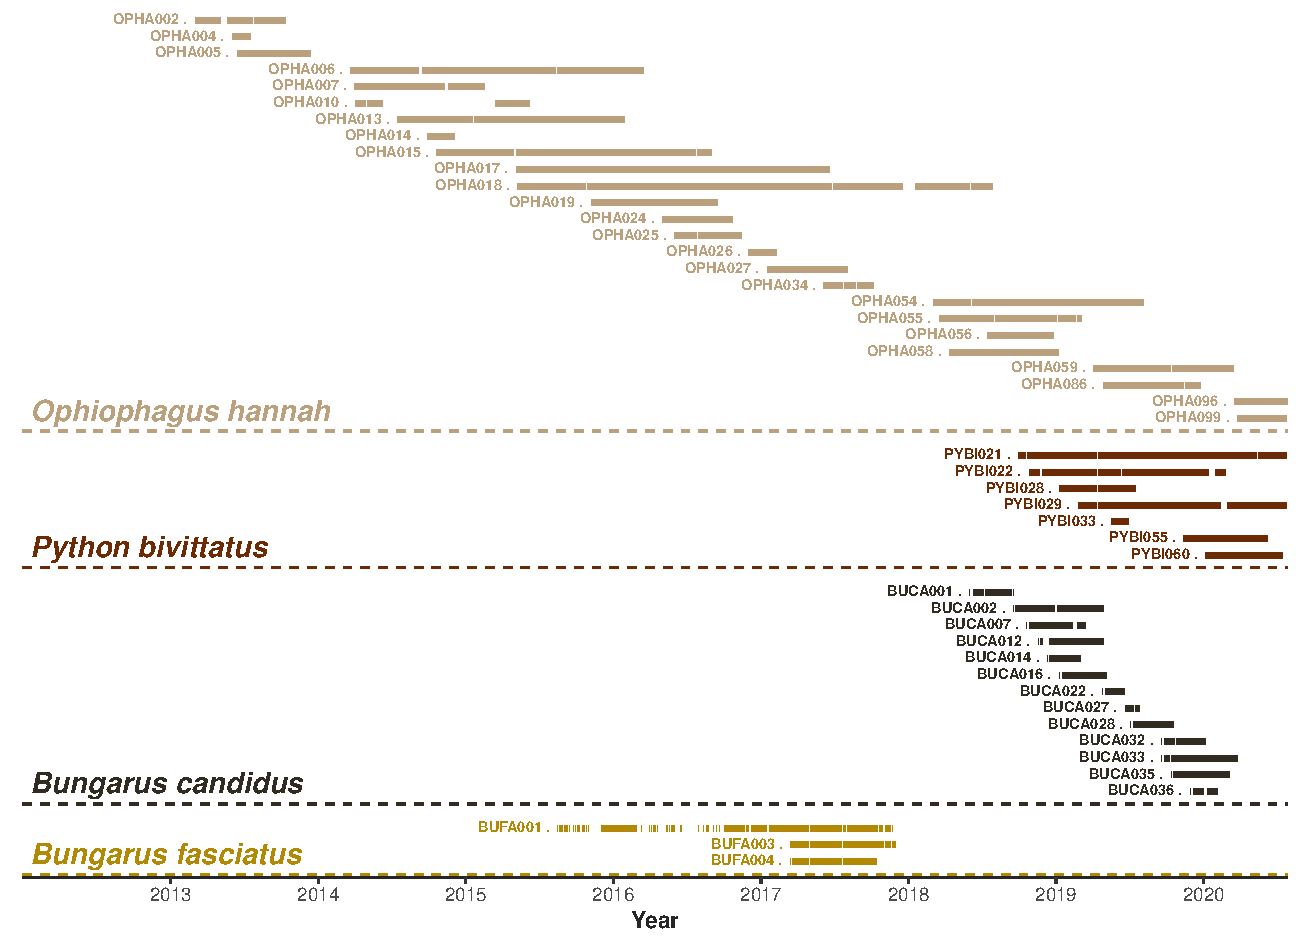
\includegraphics[width=1\linewidth]{../../figures/timeLinePlot} \caption{The time ling of all tracked individuals, split by species. Each recorded data point is depcited by a |.}\label{fig:timeLinePlot}
\end{figure}

\subsection{Species-by-hypothesis Habitat Classification}\label{species-by-hypothesis-habitat-classification}

\begin{figure}
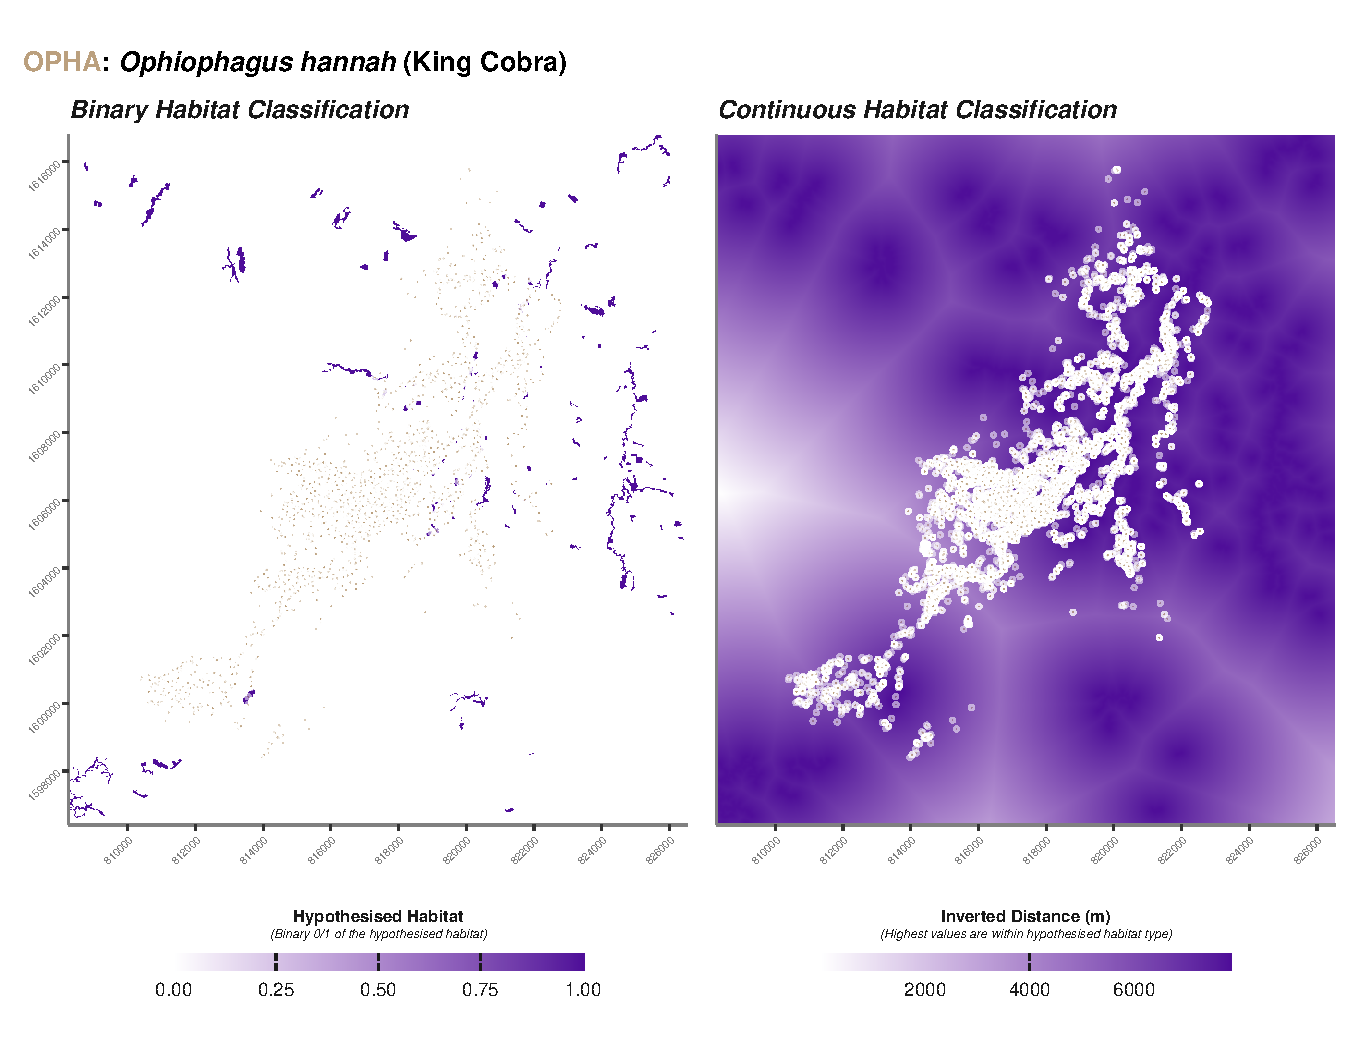
\includegraphics[width=1\linewidth]{../../figures/landscape_plot_OPHA_H1} \caption{The landscape covariates used in the King Cobra models for hypothesis 1, overlayed with the recorded locations of the animals. Left hand: the binary classification were hypothesised habitats are classed as 1, whereas all other areas are classed as 0. Right hand: the inverted continuous landscape classification where higher values indicated proximity to a given land use or habitat.}\label{fig:landscapePlotOPHA1}
\end{figure}

\begin{figure}
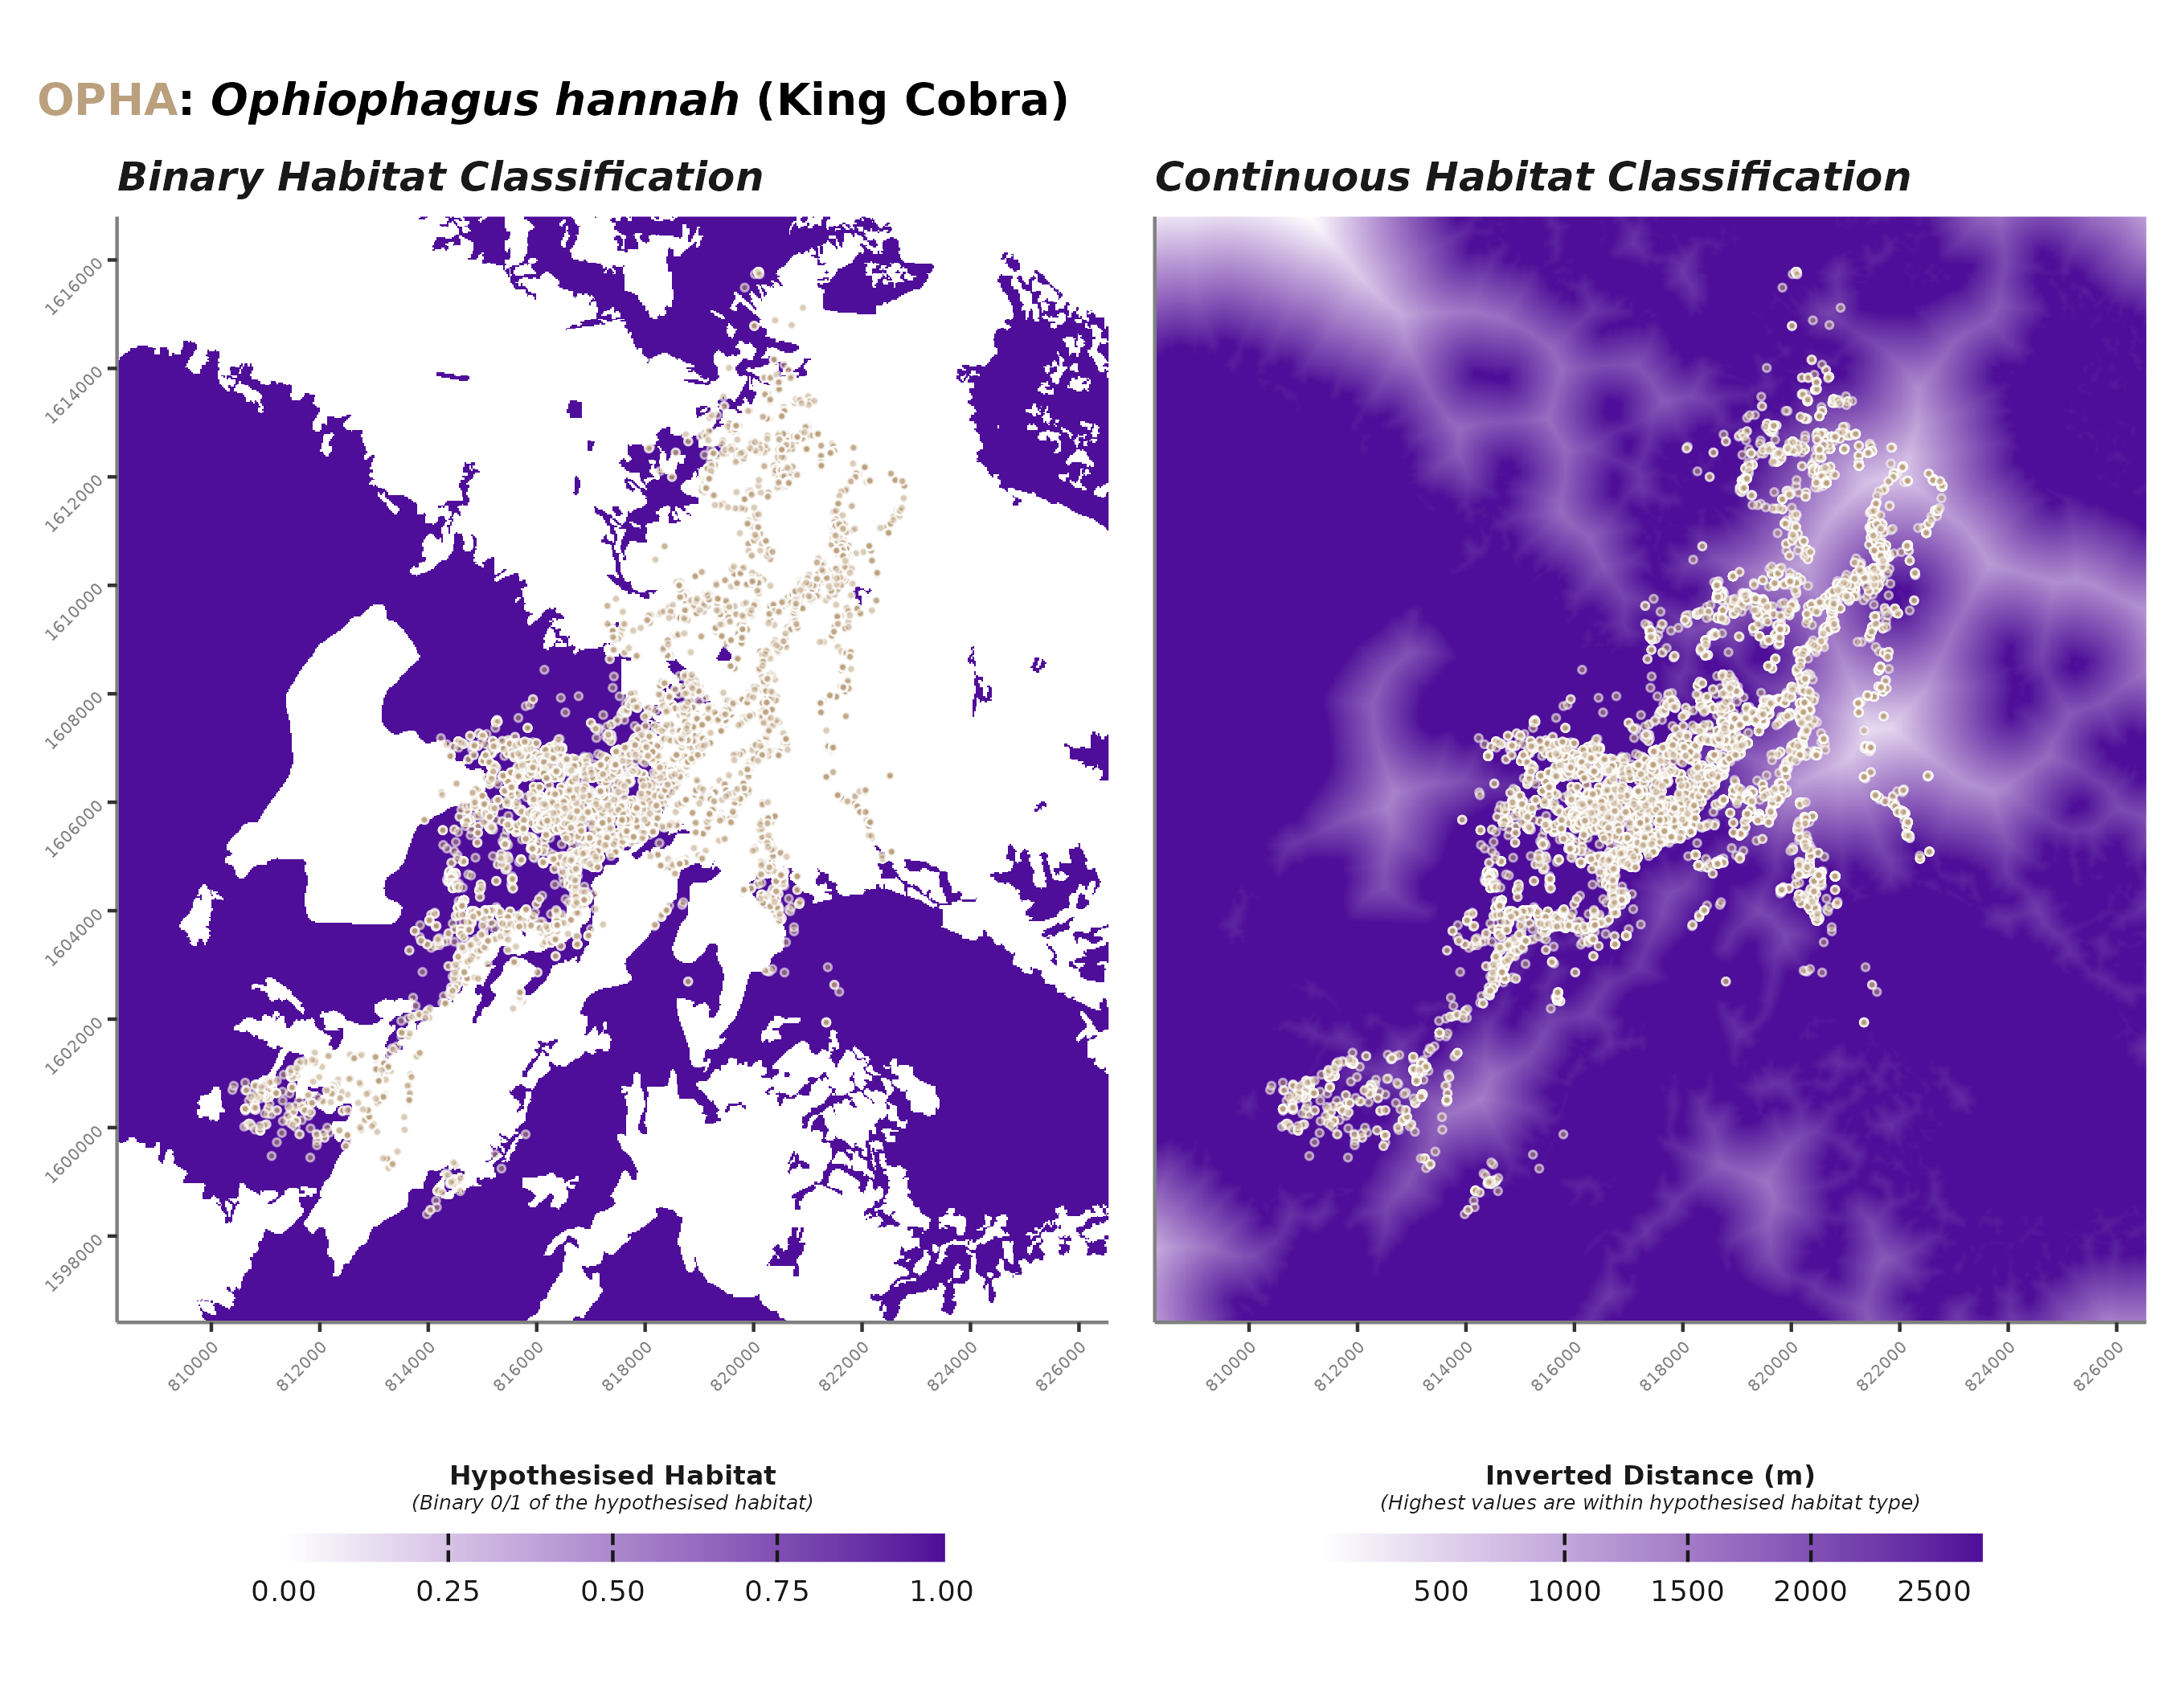
\includegraphics[width=1\linewidth]{../../figures/landscape_plot_OPHA_H2} \caption{The landscape covariates used in the King Cobra models for hypothesis 2, overlayed with the recorded locations of the animals. Left hand: the binary classification were hypothesised habitats are classed as 1, whereas all other areas are classed as 0. Right hand: the inverted continuous landscape classification where higher values indicated proximity to a given land use or habitat.}\label{fig:landscapePlotOPHA2}
\end{figure}

\begin{figure}
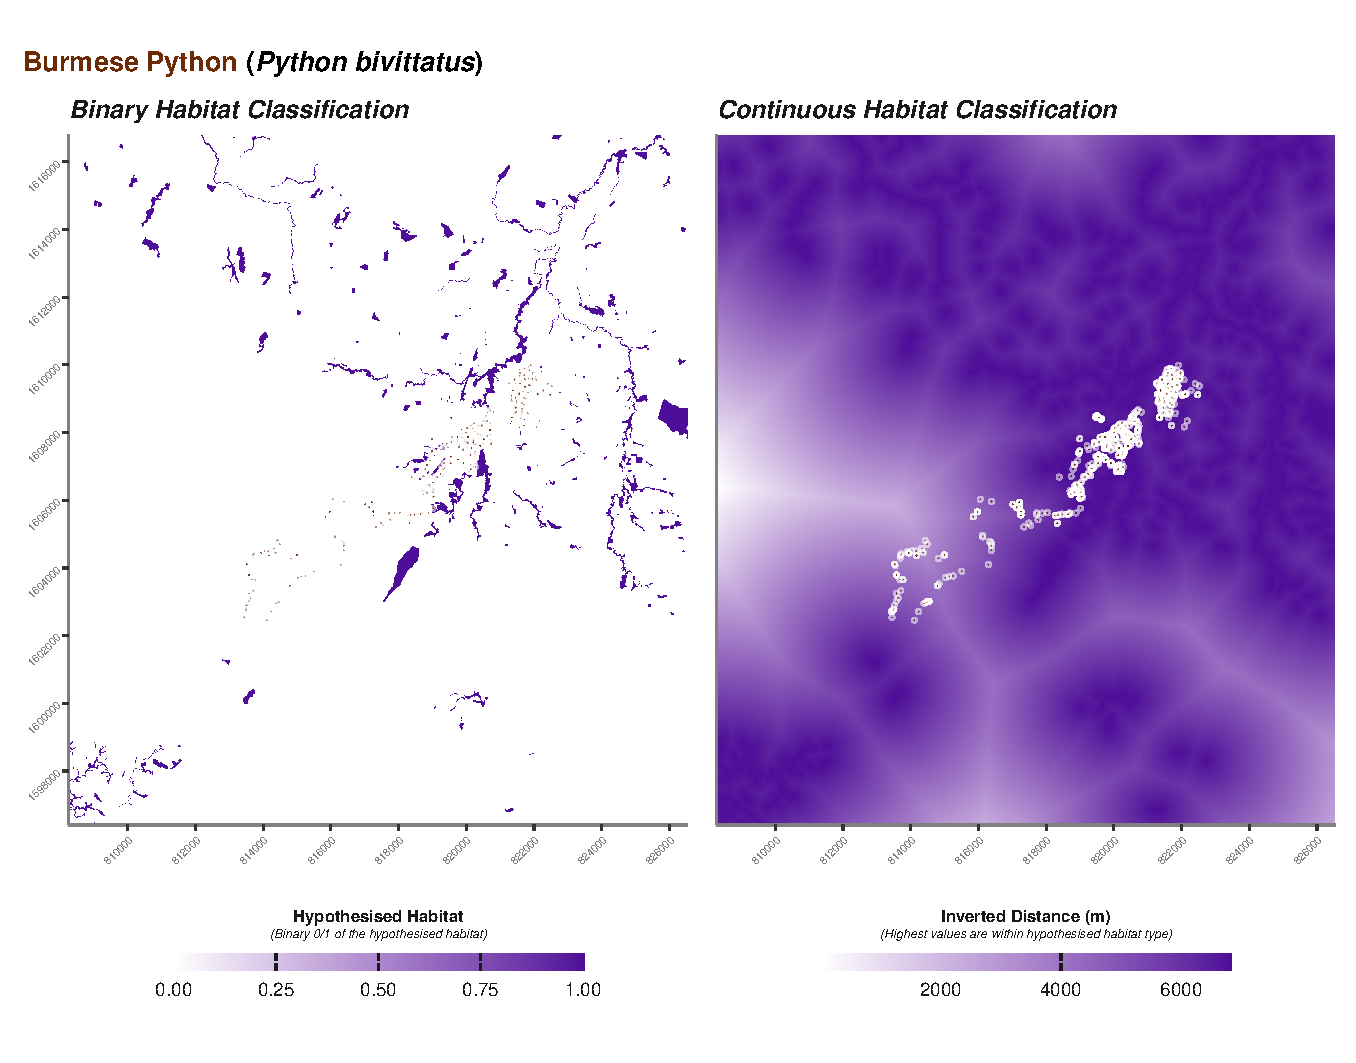
\includegraphics[width=1\linewidth]{../../figures/landscape_plot_PYBI_H1} \caption{The landscape covariates used in the Burmese Python models for hypothesis 1, overlayed with the recorded locations of the animals. Left hand: the binary classification were hypothesised habitats are classed as 1, whereas all other areas are classed as 0. Right hand: the inverted continuous landscape classification where higher values indicated proximity to a given land use or habitat.}\label{fig:landscapePlotPYBI1}
\end{figure}

\begin{figure}
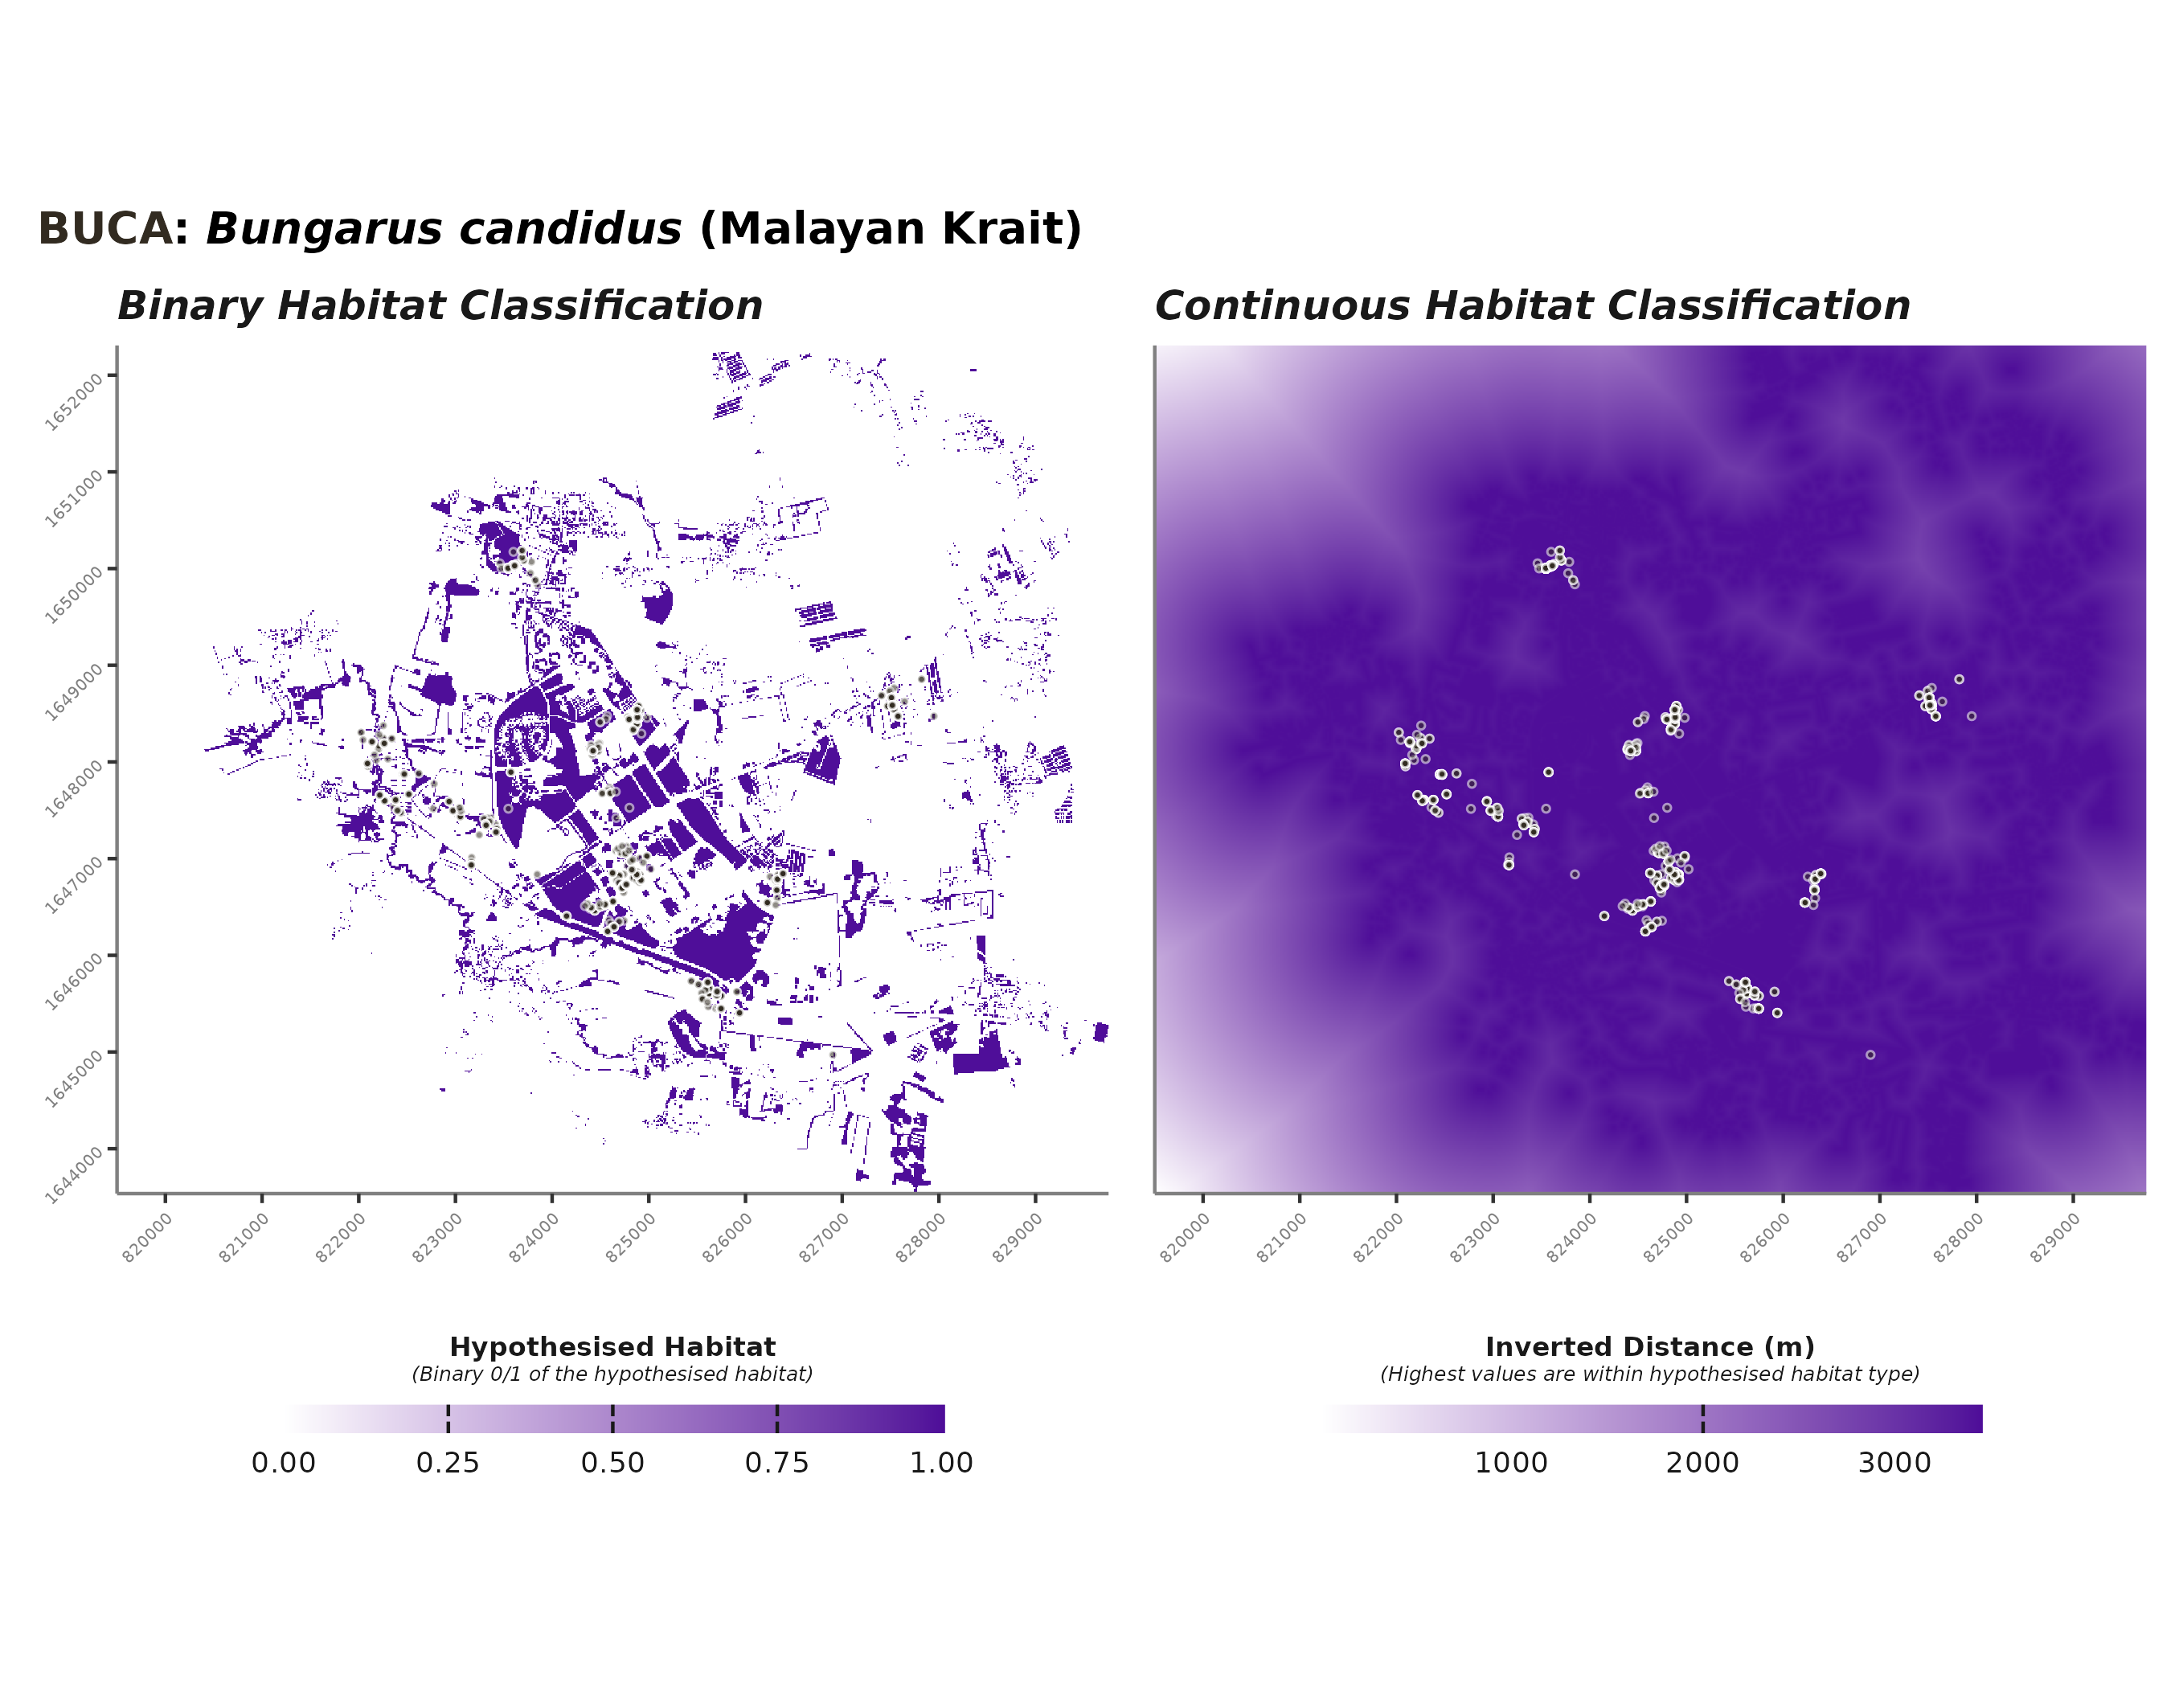
\includegraphics[width=1\linewidth]{../../figures/landscape_plot_BUCA_H1} \caption{The landscape covariates used in the Malayan Krait models for hypothesis 1, overlayed with the recorded locations of the animals. Left hand: the binary classification were hypothesised habitats are classed as 1, whereas all other areas are classed as 0. Right hand: the inverted continuous landscape classification where higher values indicated proximity to a given land use or habitat.}\label{fig:landscapePlotBUCA1}
\end{figure}

\begin{figure}
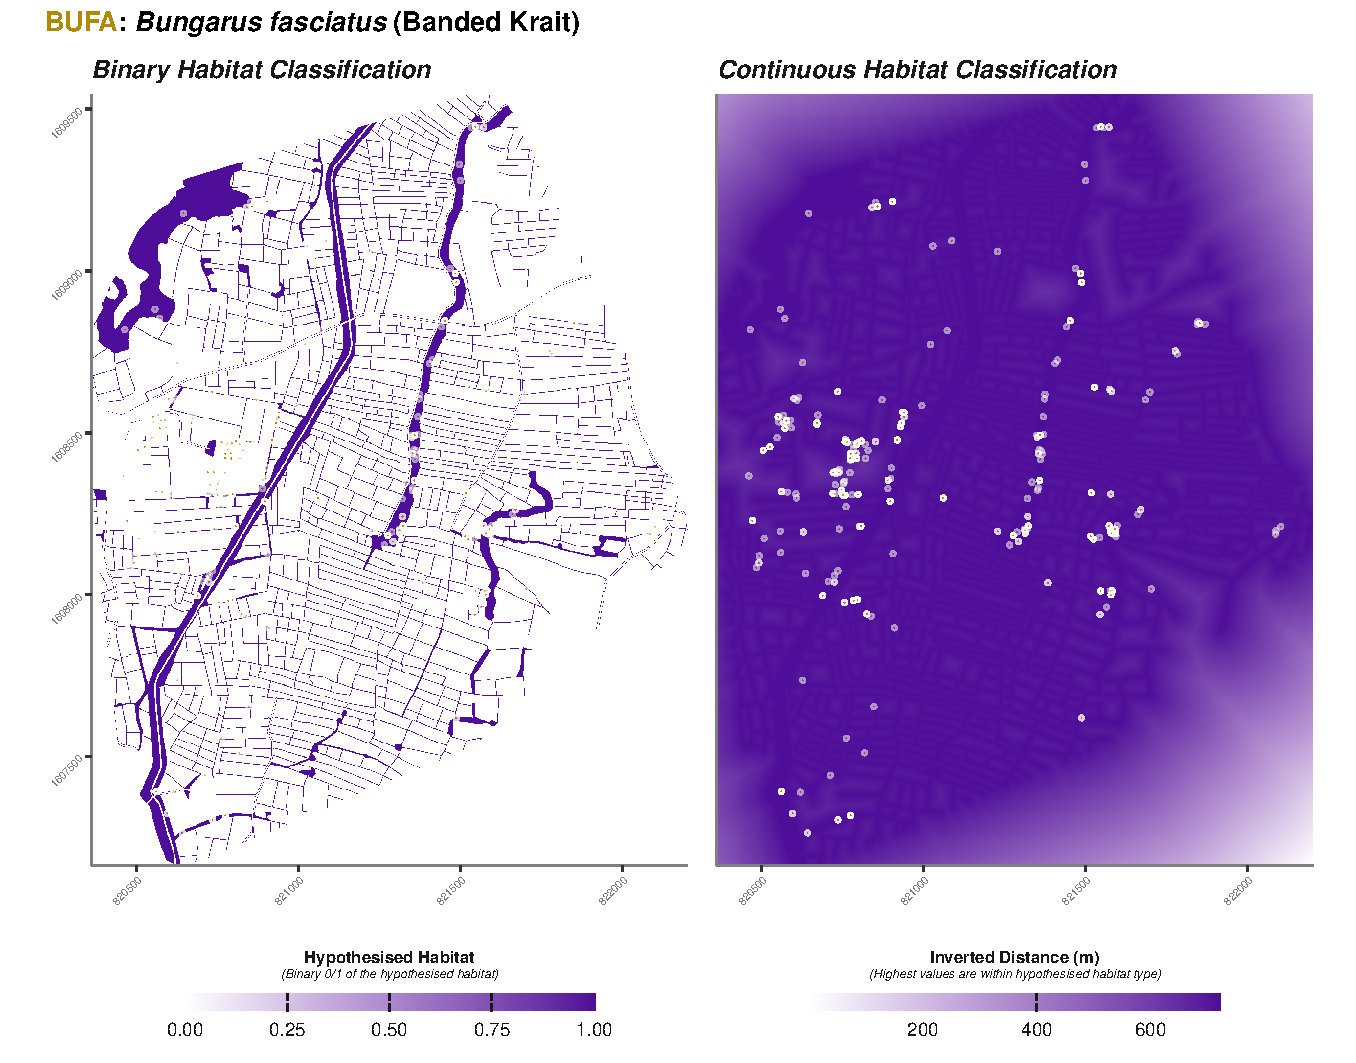
\includegraphics[width=1\linewidth]{../../figures/landscape_plot_BUFA_H1} \caption{The landscape covariates used in the Banded Krait models for hypothesis 1, overlayed with the recorded locations of the animals. Left hand: the binary classification were hypothesised habitats are classed as 1, whereas all other areas are classed as 0. Right hand: the inverted continuous landscape classification where higher values indicated proximity to a given land use or habitat.}\label{fig:landscapePlotBUFA1}
\end{figure}

\subsection{Species-by-species Specification Curves}\label{species-by-species-specification-curves}

\subsubsection{\texorpdfstring{King Cobra (\emph{Ophiophagus hannah})}{King Cobra (Ophiophagus hannah)}}\label{king-cobra-ophiophagus-hannah}

\begin{figure}
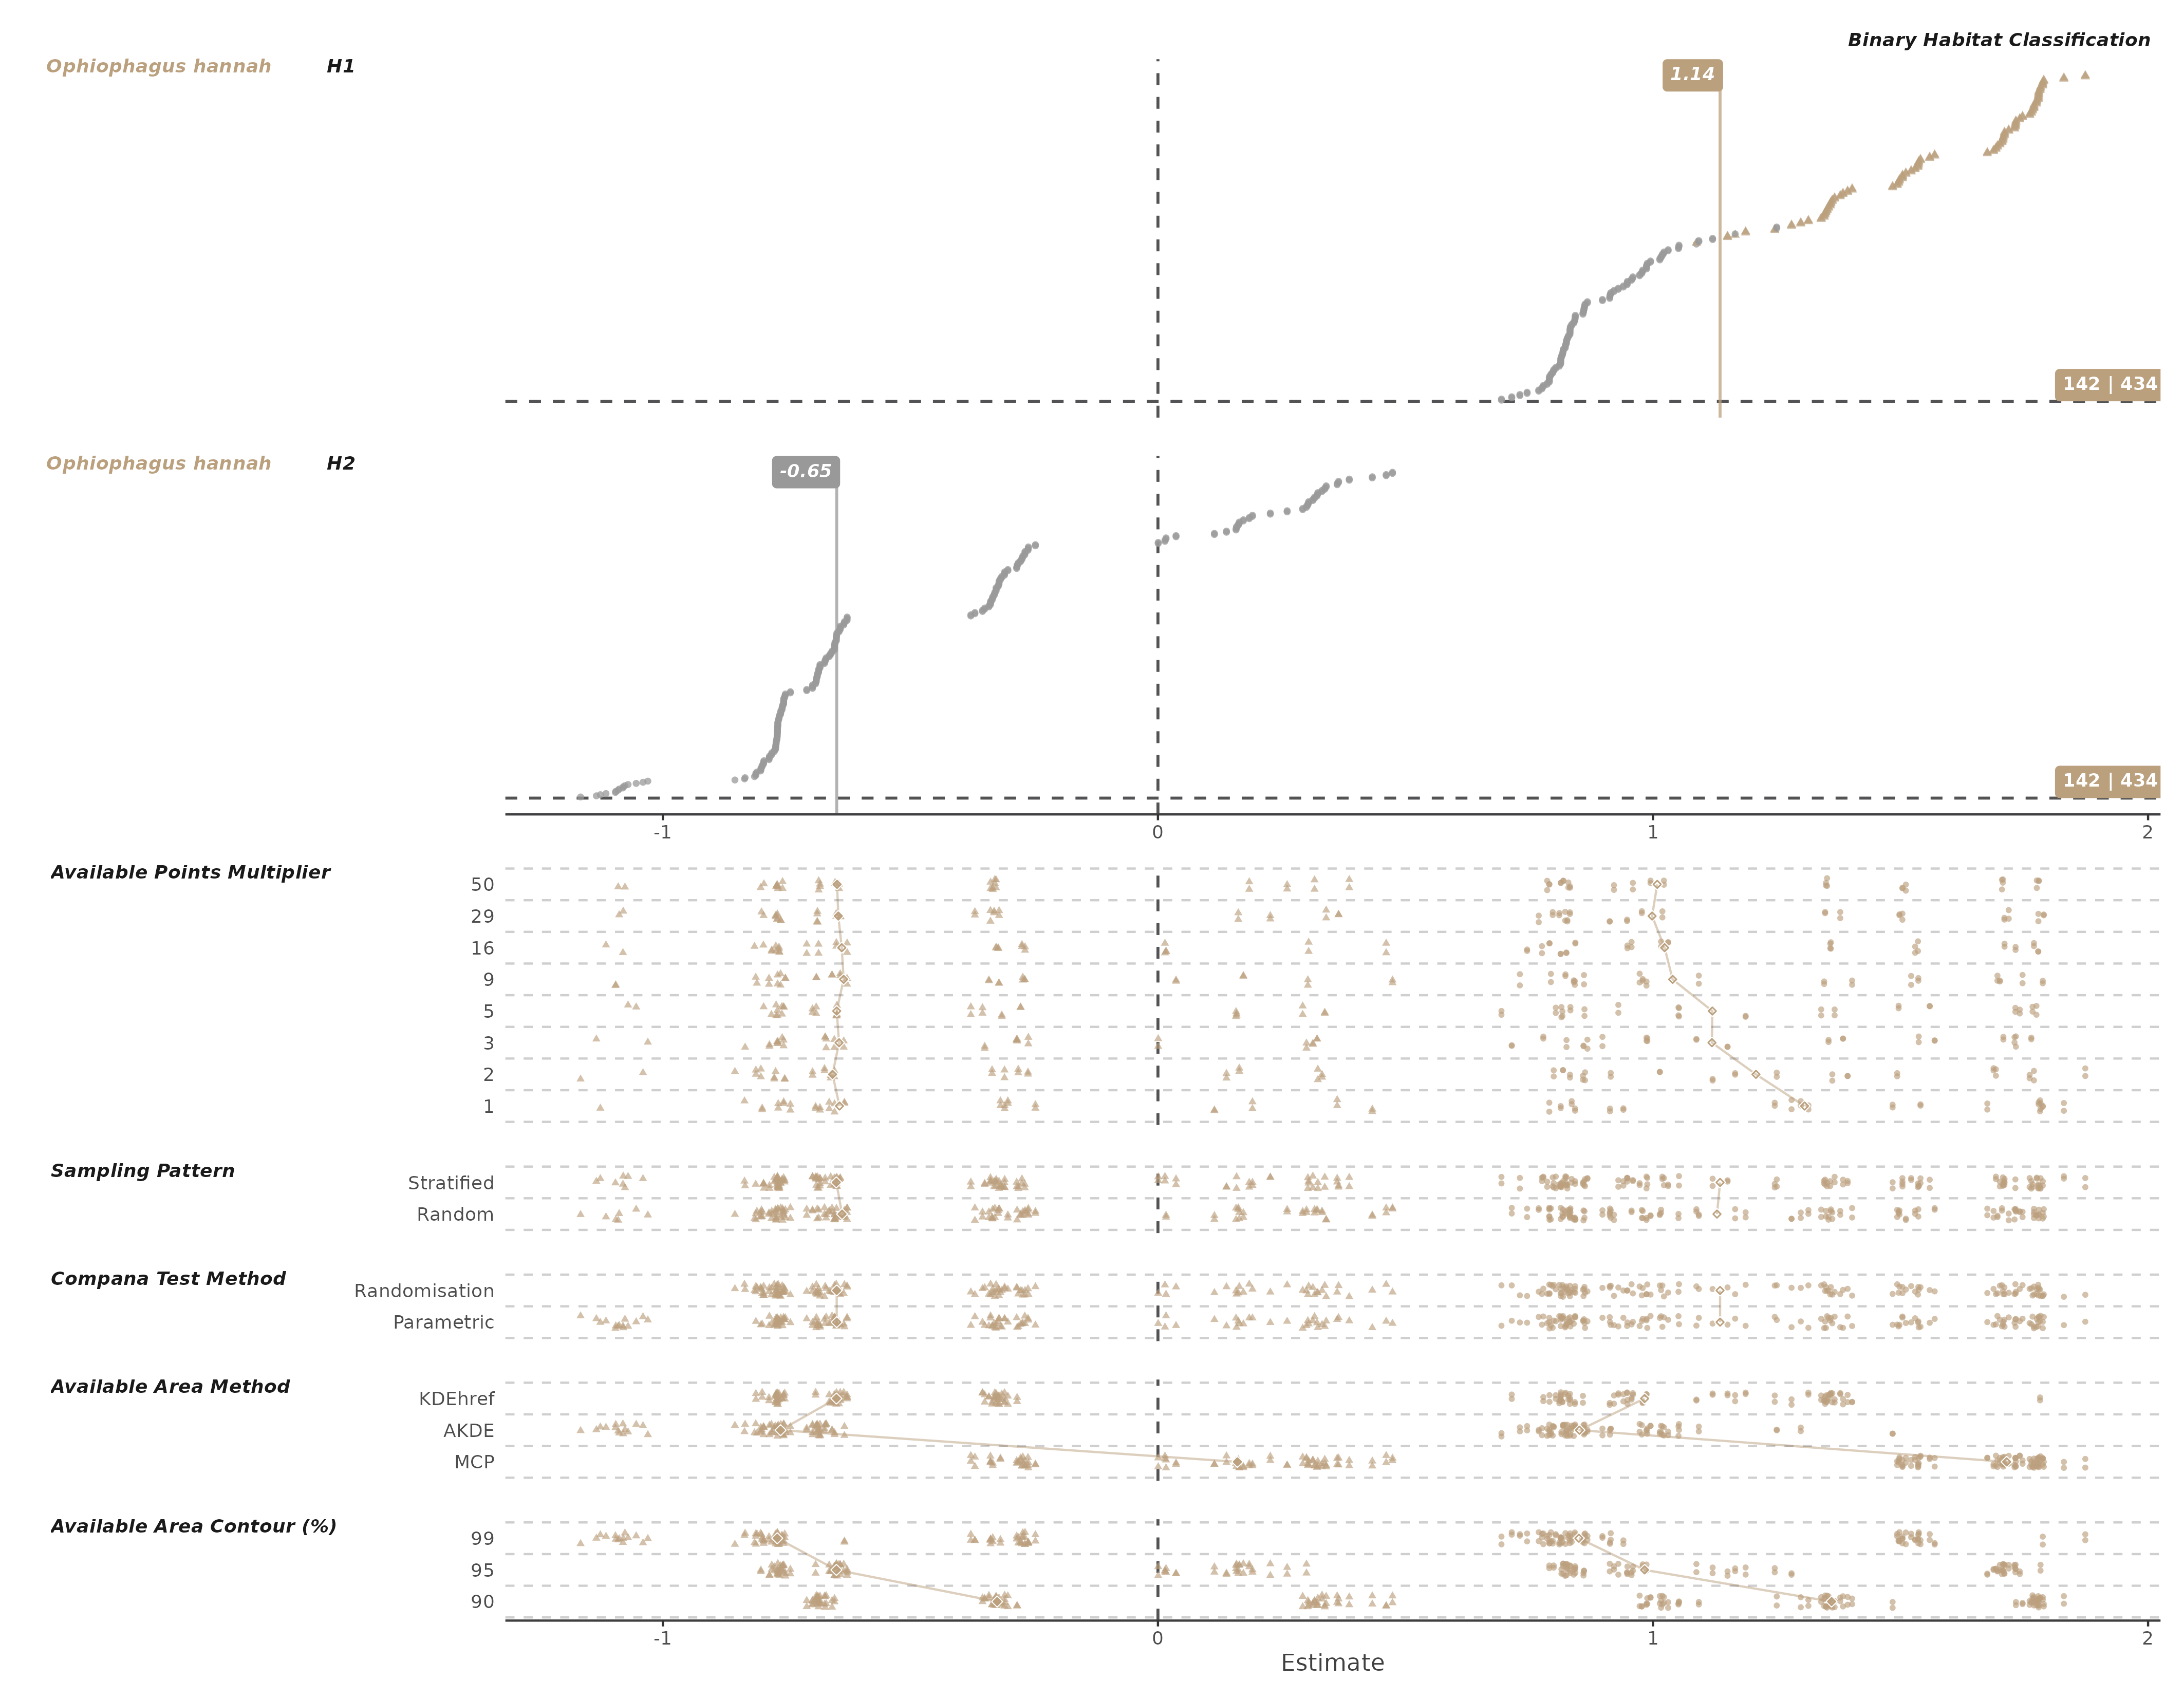
\includegraphics[width=1\linewidth]{../../figures/specCurve_Ophiophagus hannah_area} \caption{All estimates of habitat selection derived from the areas-based Compositional (Compana) analysis for Banded Kraits (Ophiophagus hannah). Top curves show all estimates with coloured points and corresponding confidence intervals indicating whether those estimates significantly support the hypothesis. Bottom right labels provide a count of estimates that significantly support the hypothesis out of the total estimates. Labelled vertical lines show the median point estimate. Lower plot show the estimates relative to each analysis choice. Median estimates are shown with hollow diamonds, and are connected with appropriated coloured lines. Shape separate hypothesis 1 and 2 (circles = hypothesis 1, triangle = hypothesis 2). Median estimates are shown with hollow diamonds, and hypothesis medians are connected with appropriated coloured lines. }\label{fig:specCurveAreaOPHA}
\end{figure}

\begin{figure}
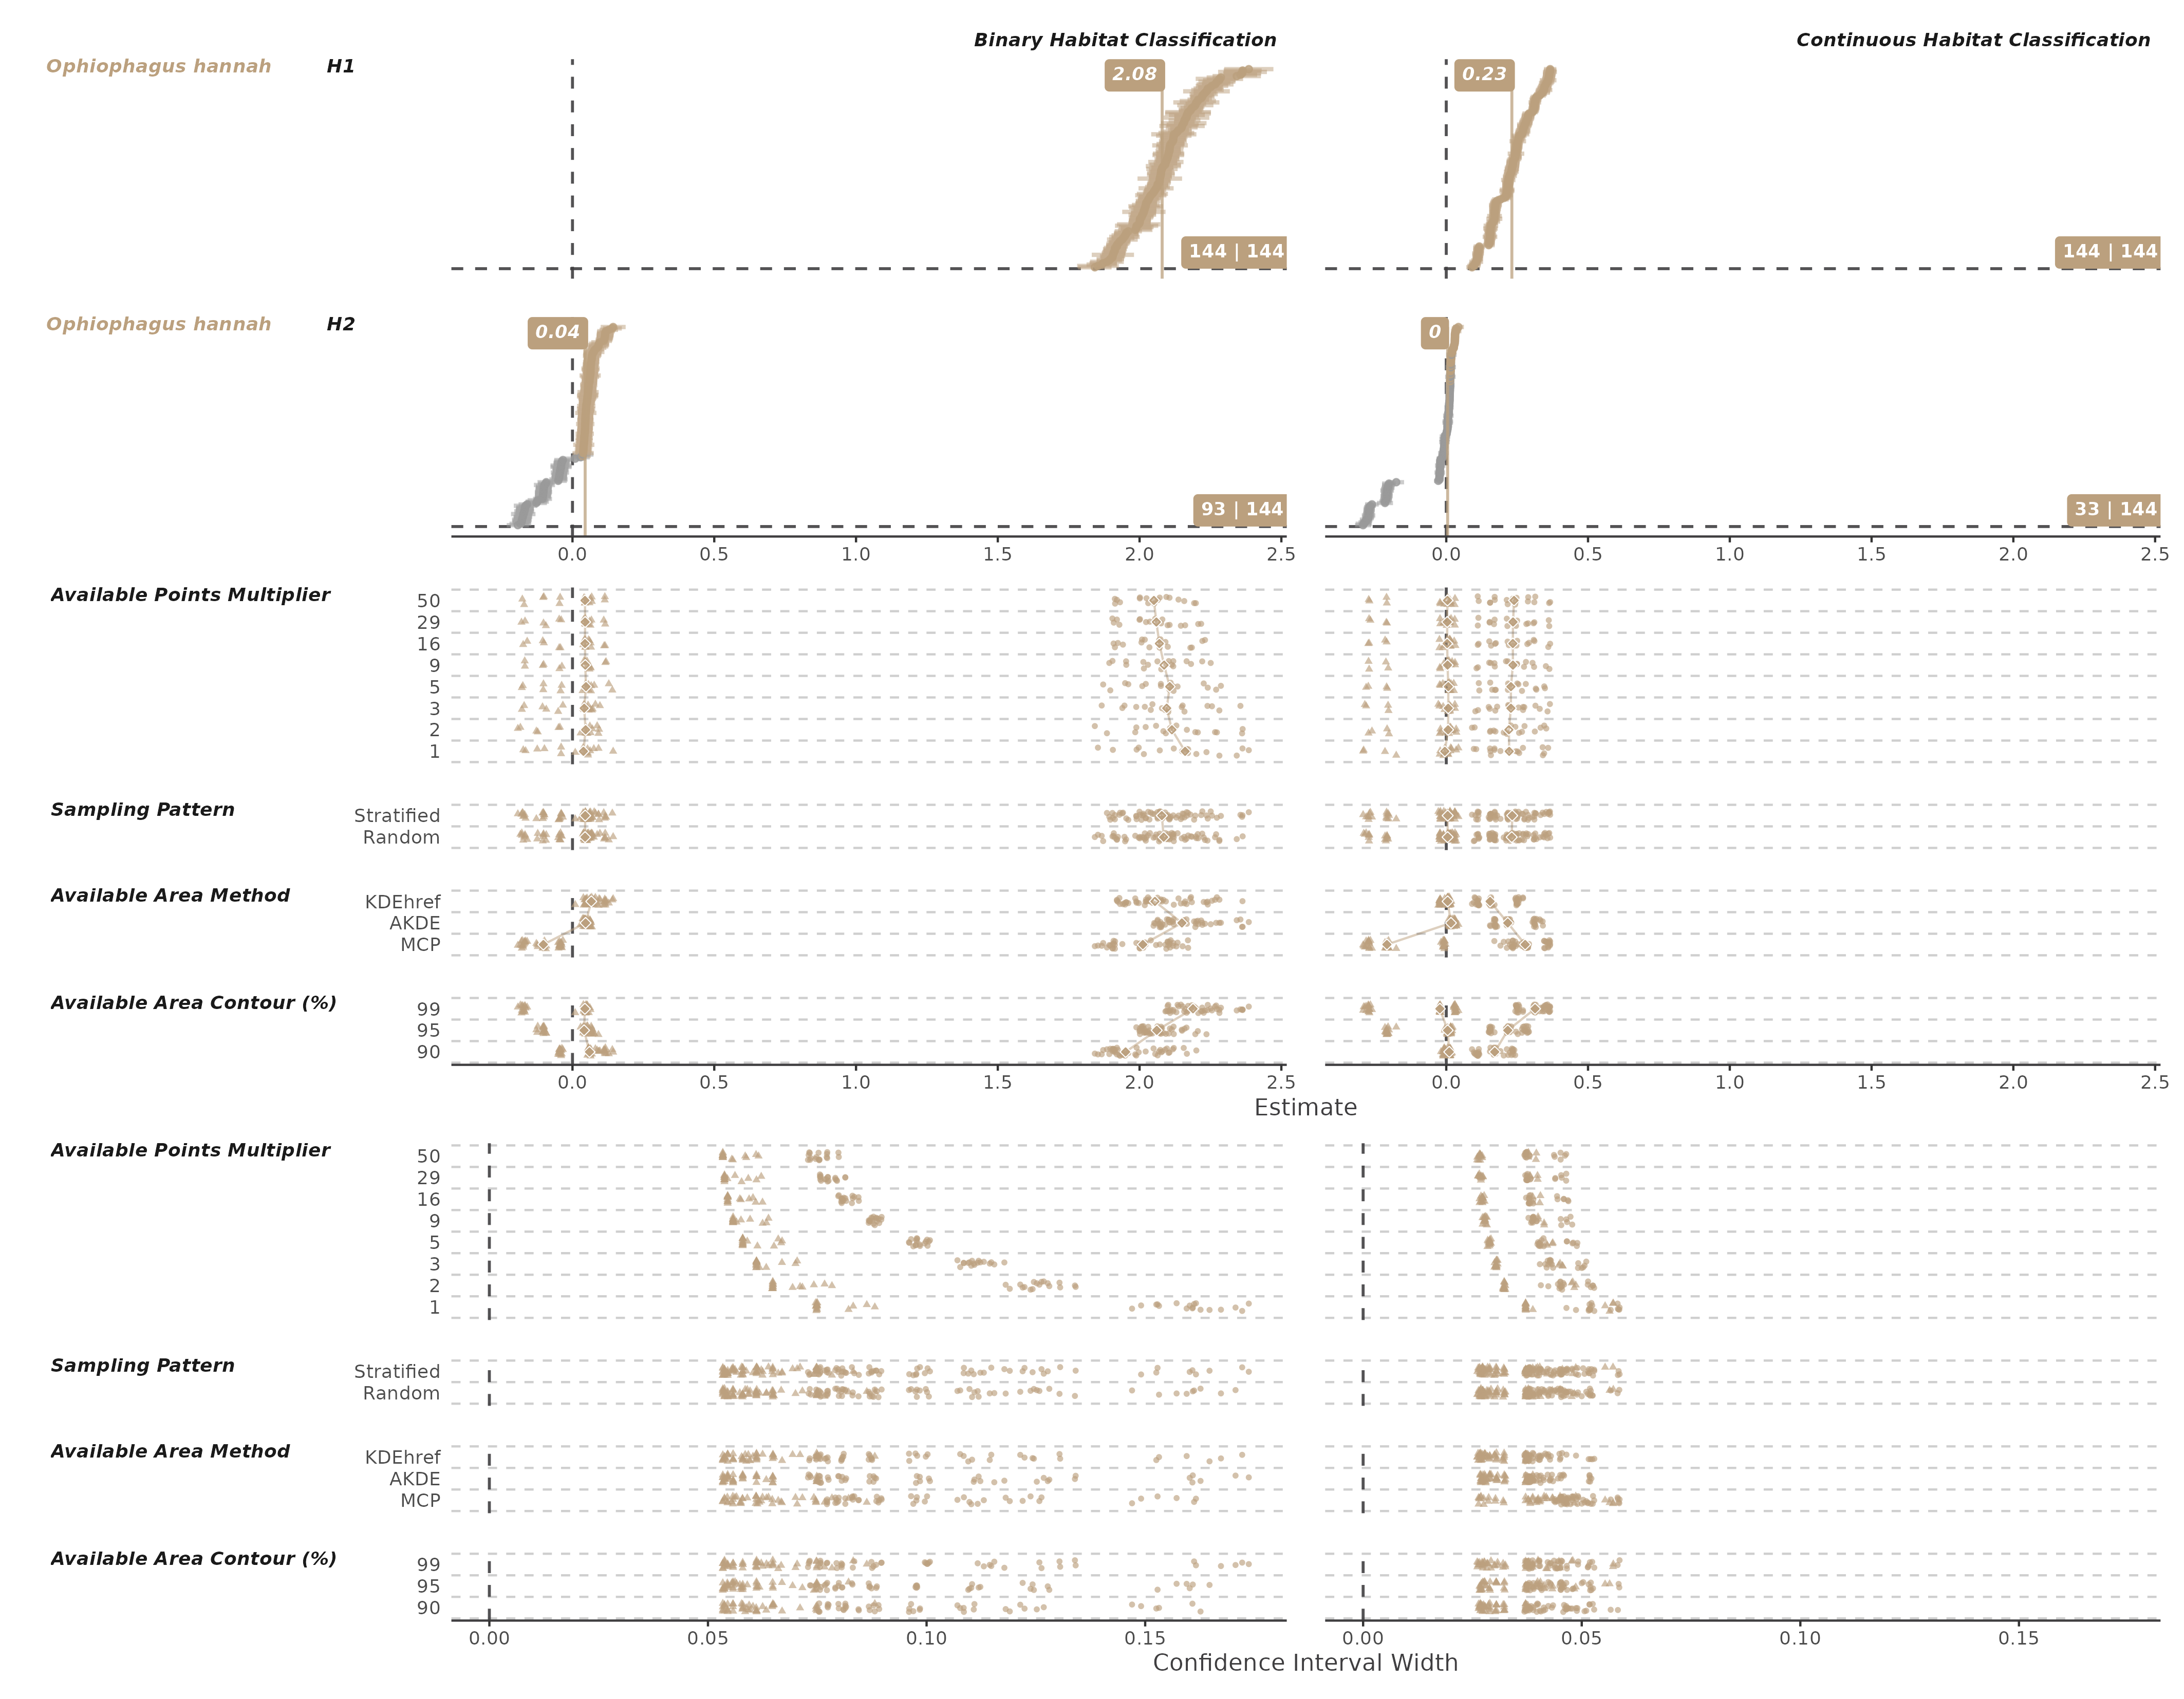
\includegraphics[width=1\linewidth]{../../figures/specCurve_Ophiophagus hannah_rsf} \caption{All estimates of habitat selection derived from the areas-based Resource Selection Function (RSF) analysis for Banded Kraits (Ophiophagus hannah). Top curves show all estimates with coloured points and corresponding confidence intervals indicating whether those estimates significantly support the hypothesis. Bottom right labels provide a count of estimates that significantly support the hypothesis out of the total estimates. Labelled vertical lines show the median point estimate. Lower plot show the estimates relative to each analysis choice. Median estimates are shown with hollow diamonds, and are connected with appropriated coloured lines. The plot is split left and right for the analysis using a binary classification (left), and continuous inverted distance (right).}\label{fig:specCurveRsfOPHA}
\end{figure}

\begin{figure}
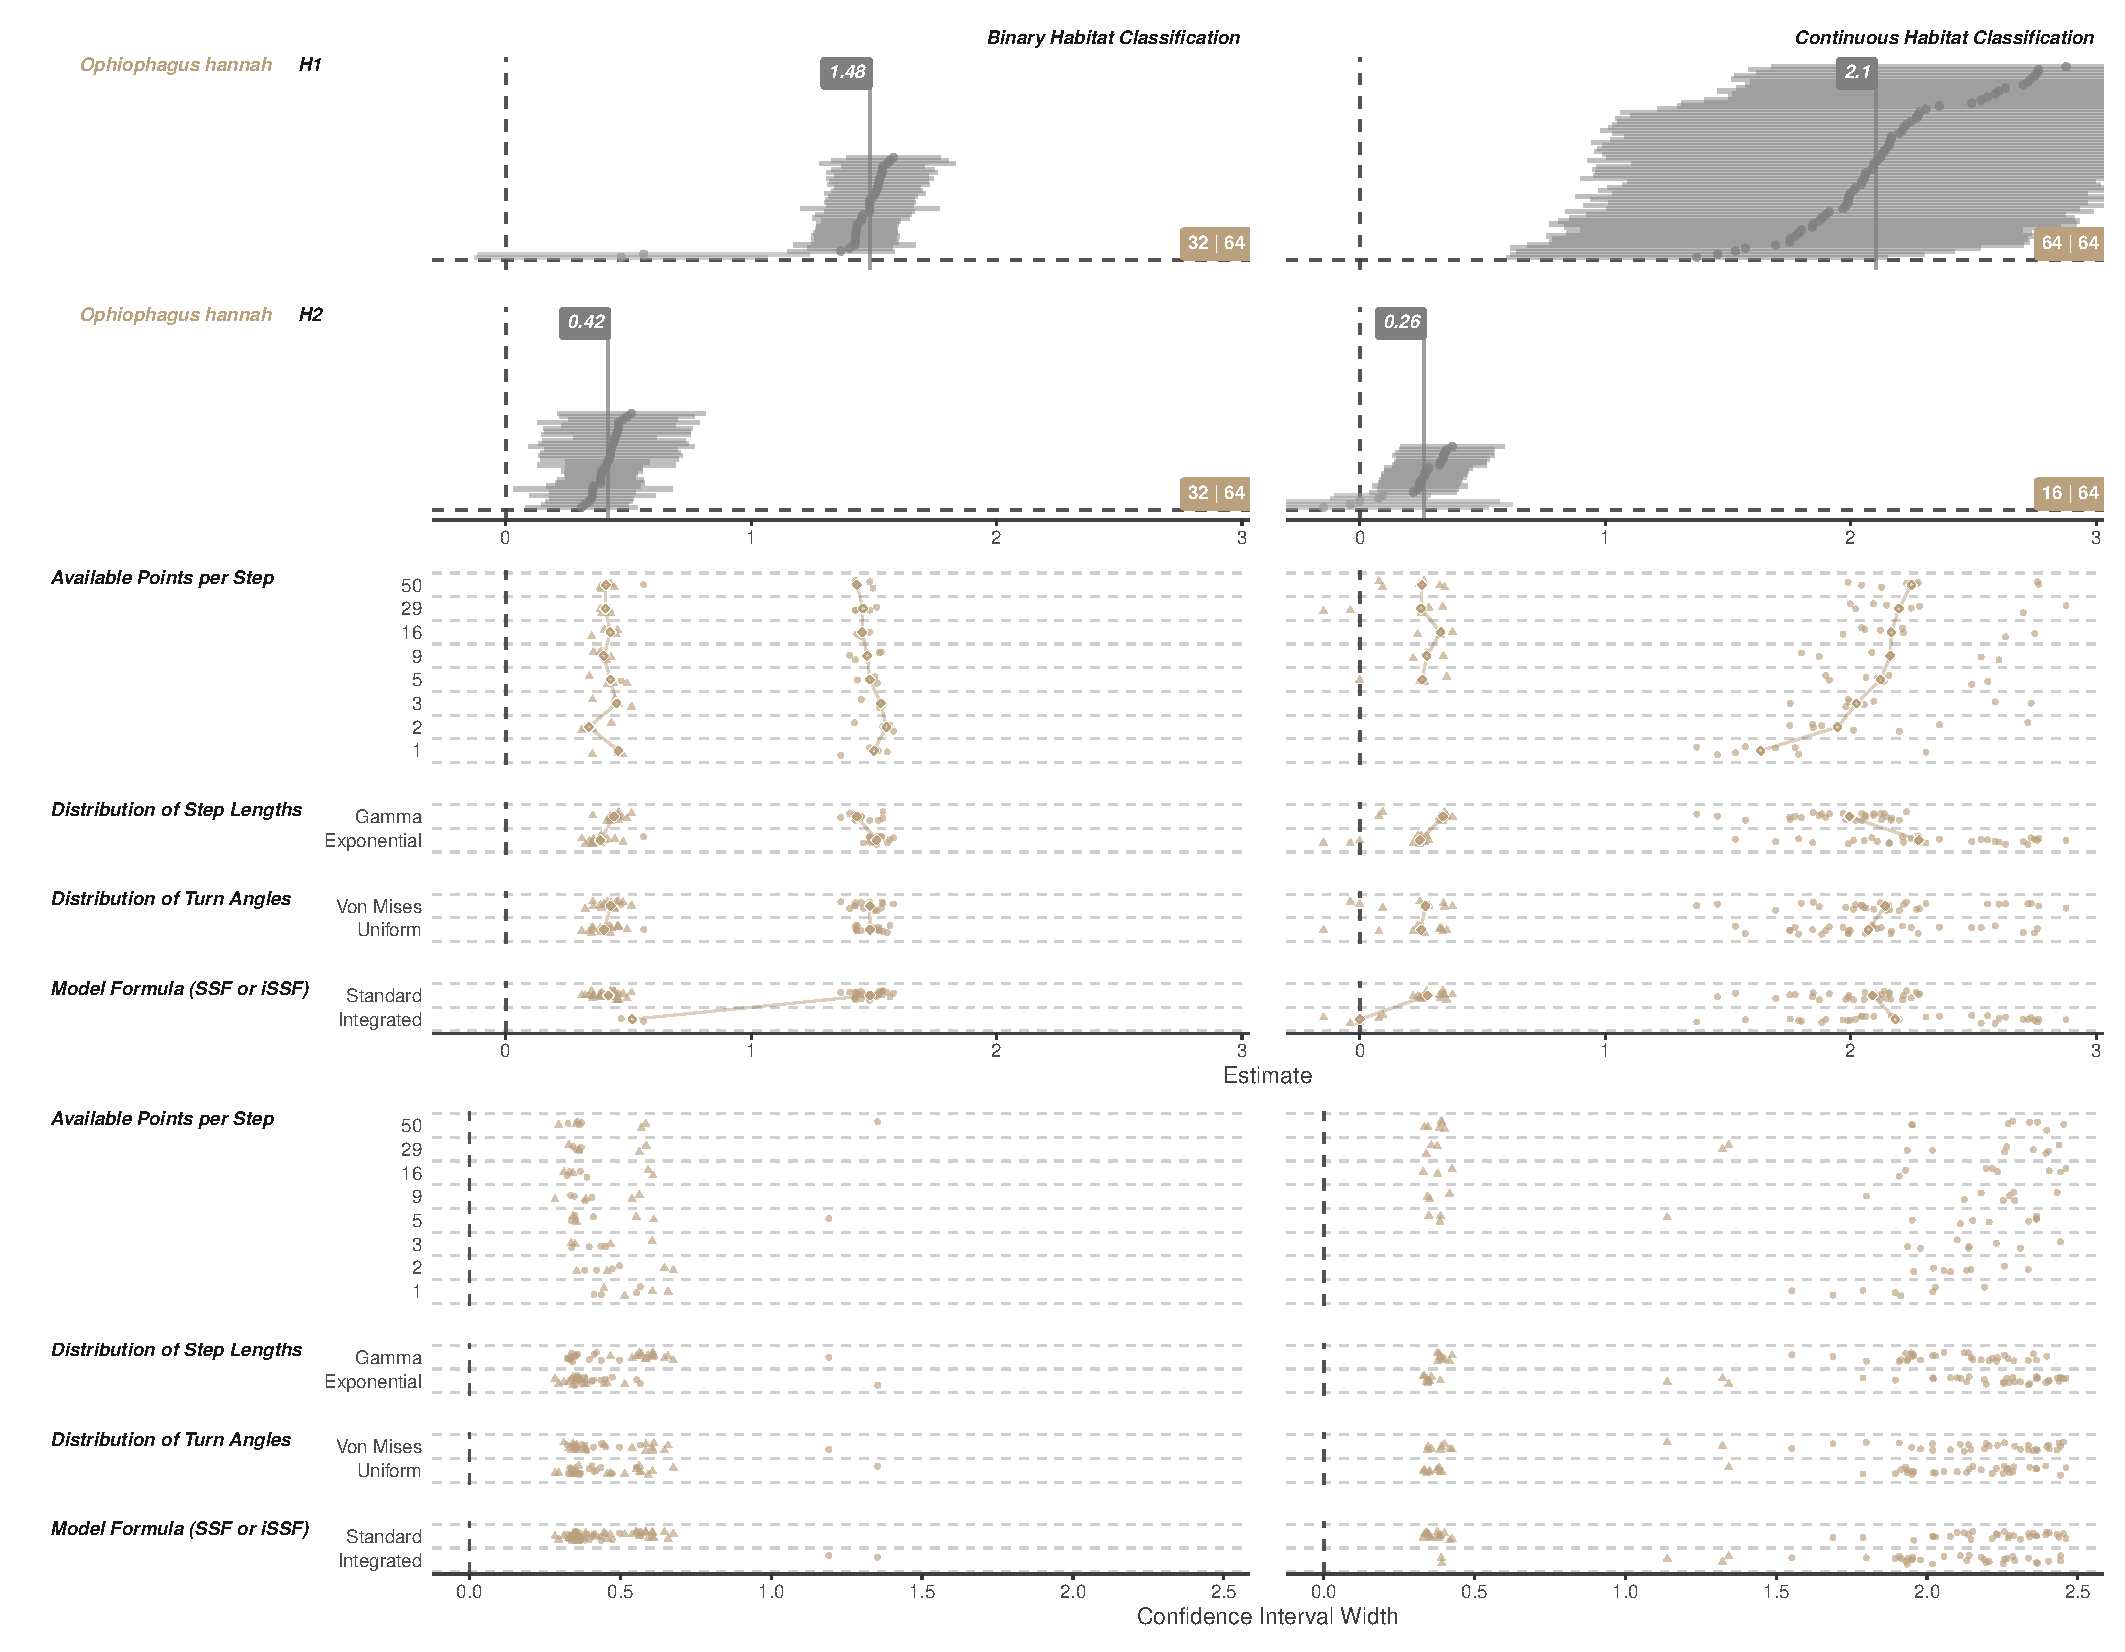
\includegraphics[width=1\linewidth]{../../figures/specCurve_Ophiophagus hannah_twoStep} \caption{All estimates of habitat selection derived from the step-based Two-Step analysis for King Cobras (Ophiophagus hannah). Top curves show all estimates, split by hypothesis, with coloured points and corresponding confidence intervals indicating whether those estimates significantly support the hypothesis. Bottom right labels provide a count of estimates that significantly support the hypothesis out of the total estimates. Labelled vertical lines show the median point estimate for each hypothesis. Lower plot show the estimates relative to each analysis choice. Shape separate hypothesis 1 and 2 (circles = hypothesis 1, triangle = hypothesis 2). Median estimates are shown with hollow diamonds, and hypothesis medians are connected with appropriated coloured lines. The plot is split left and right for the analysis using a binary classification (left), and continuous inverted distance (right).}\label{fig:specCurveTwoStepOPHA}
\end{figure}

\begin{figure}
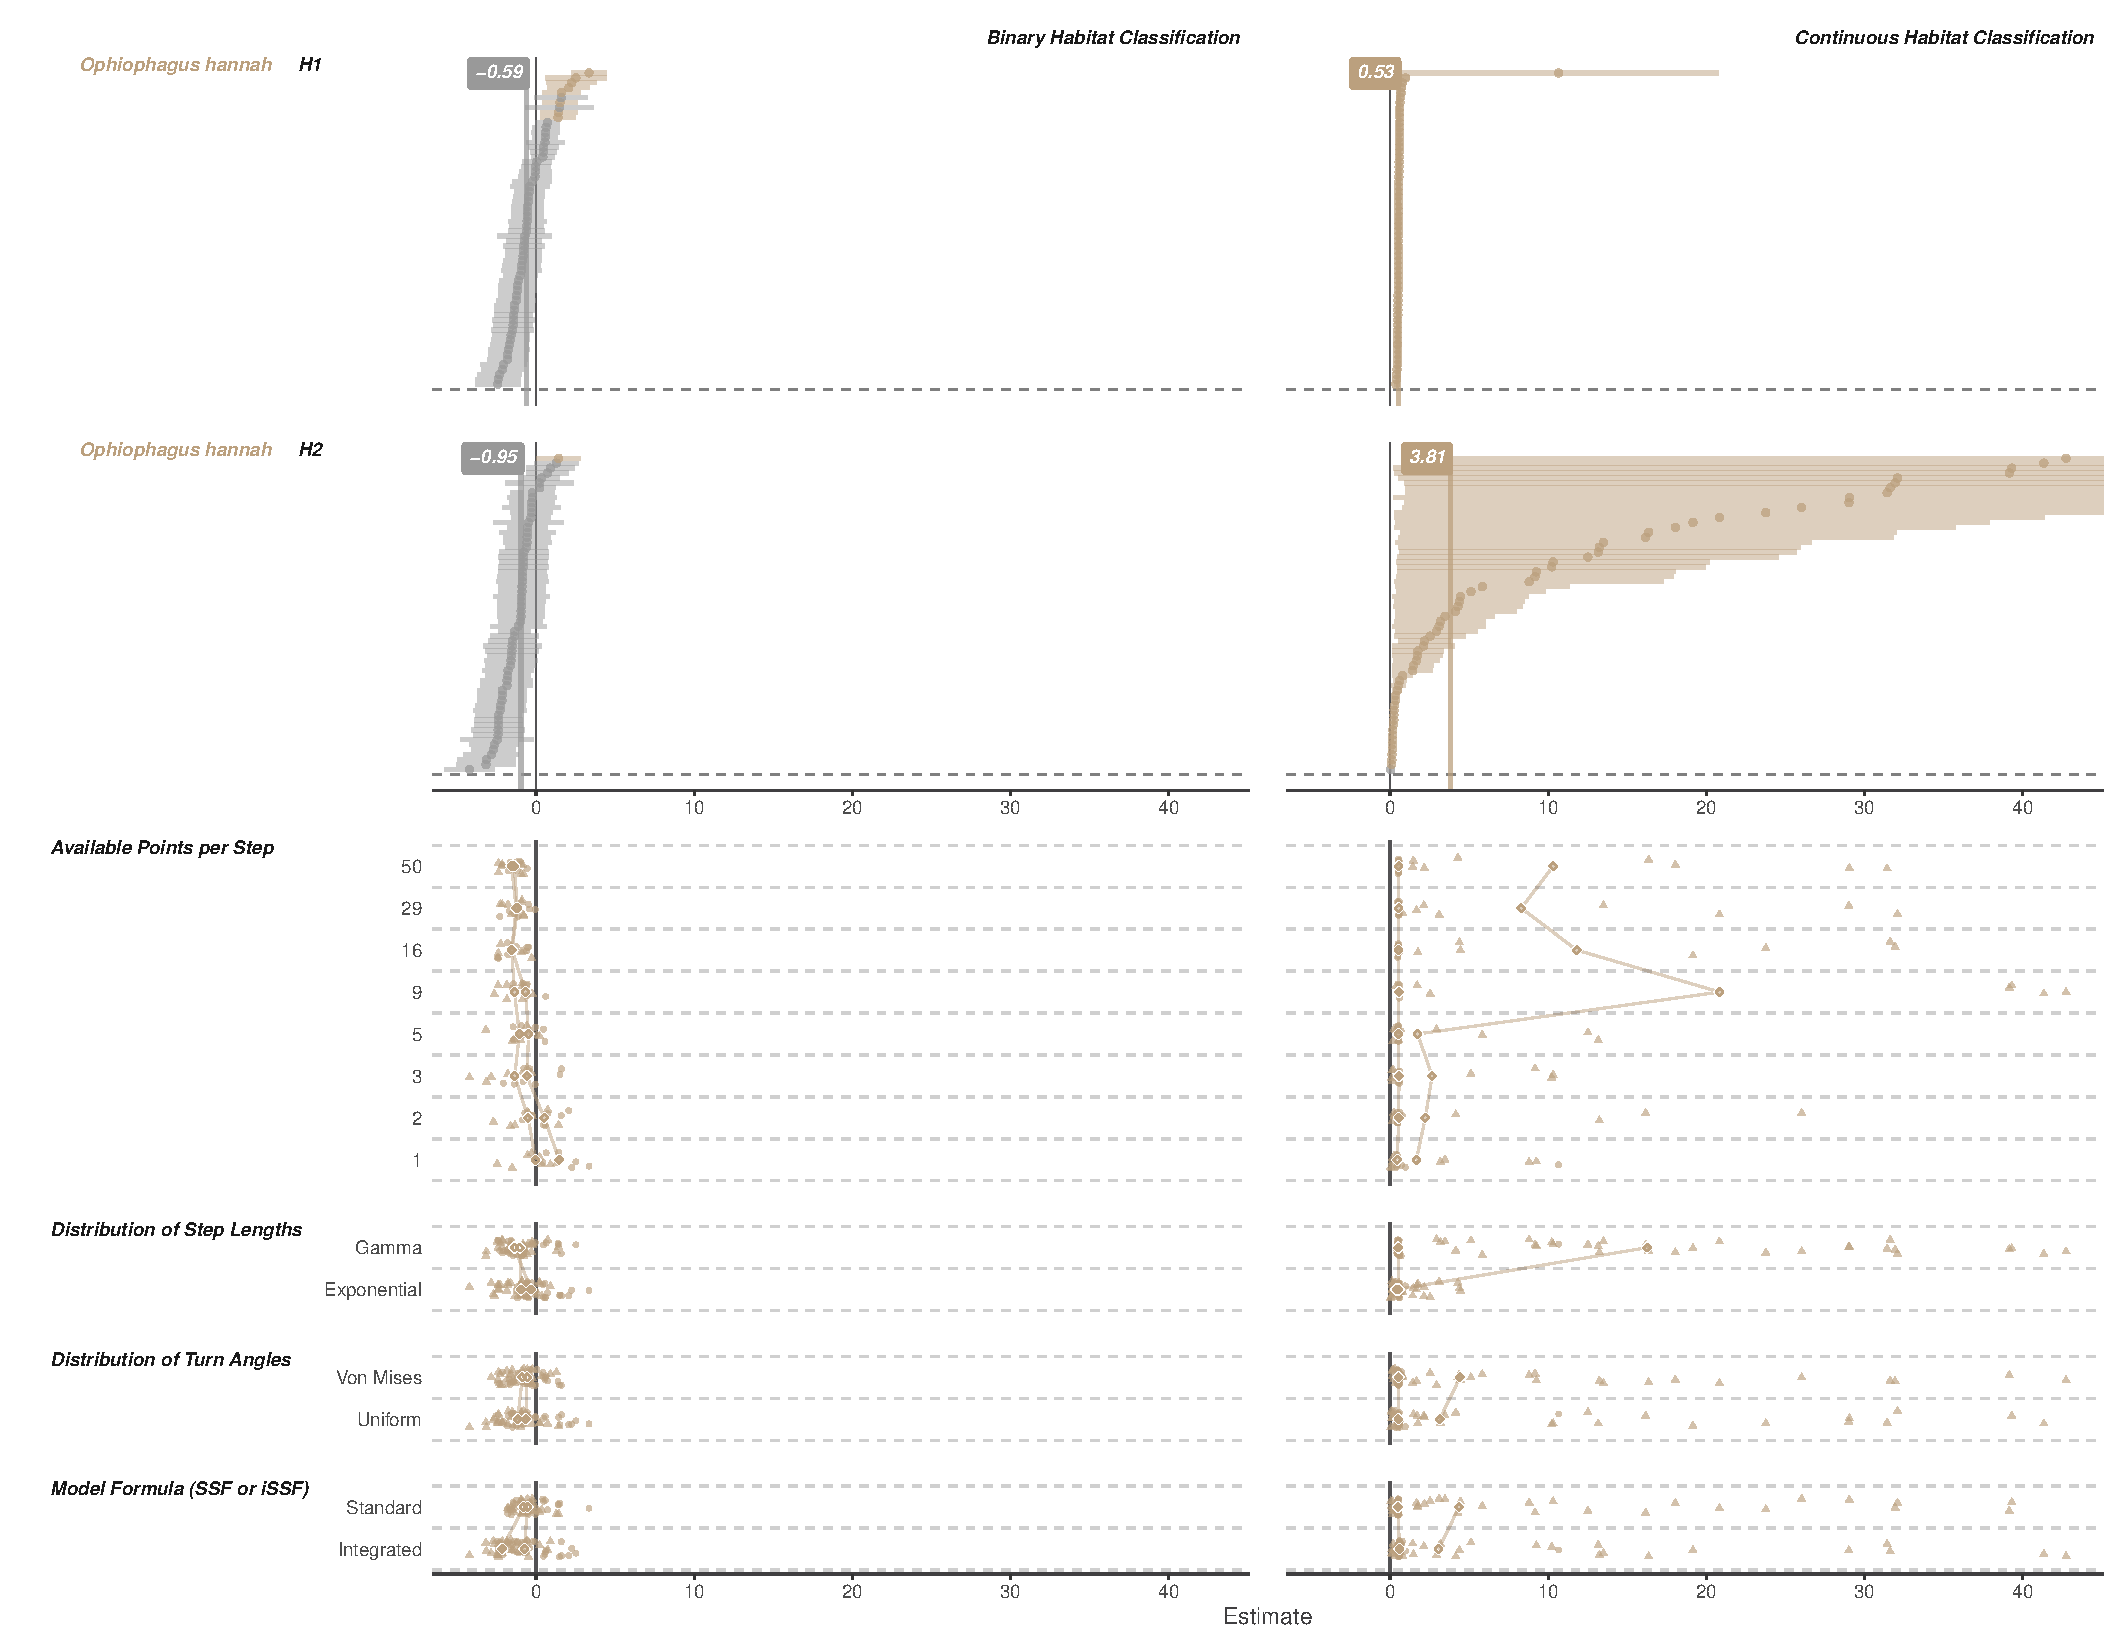
\includegraphics[width=1\linewidth]{../../figures/specCurve_Ophiophagus hannah_ssf} \caption{All estimates of habitat selection derived from the step-based Step Selection Function (SSF) analysis for King Cobras (Ophiophagus hannah). Top curves show all estimates, split by hypothesis, with coloured points and corresponding confidence intervals indicating whether those estimates significantly support the hypothesis. Bottom right labels provide a count of estimates that significantly support the hypothesis out of the total estimates. Labelled vertical lines show the median point estimate for each hypothesis. Lower plot show the estimates relative to each analysis choice. Shape separate hypothesis 1 and 2 (circles = hypothesis 1, triangle = hypothesis 2). Median estimates are shown with hollow diamonds, and hypothesis medians are connected with appropriated coloured lines. The plot is split left and right for the analysis using a binary classification (left), and continuous inverted distance (right).}\label{fig:specCurveSsfOPHA}
\end{figure}

\begin{figure}
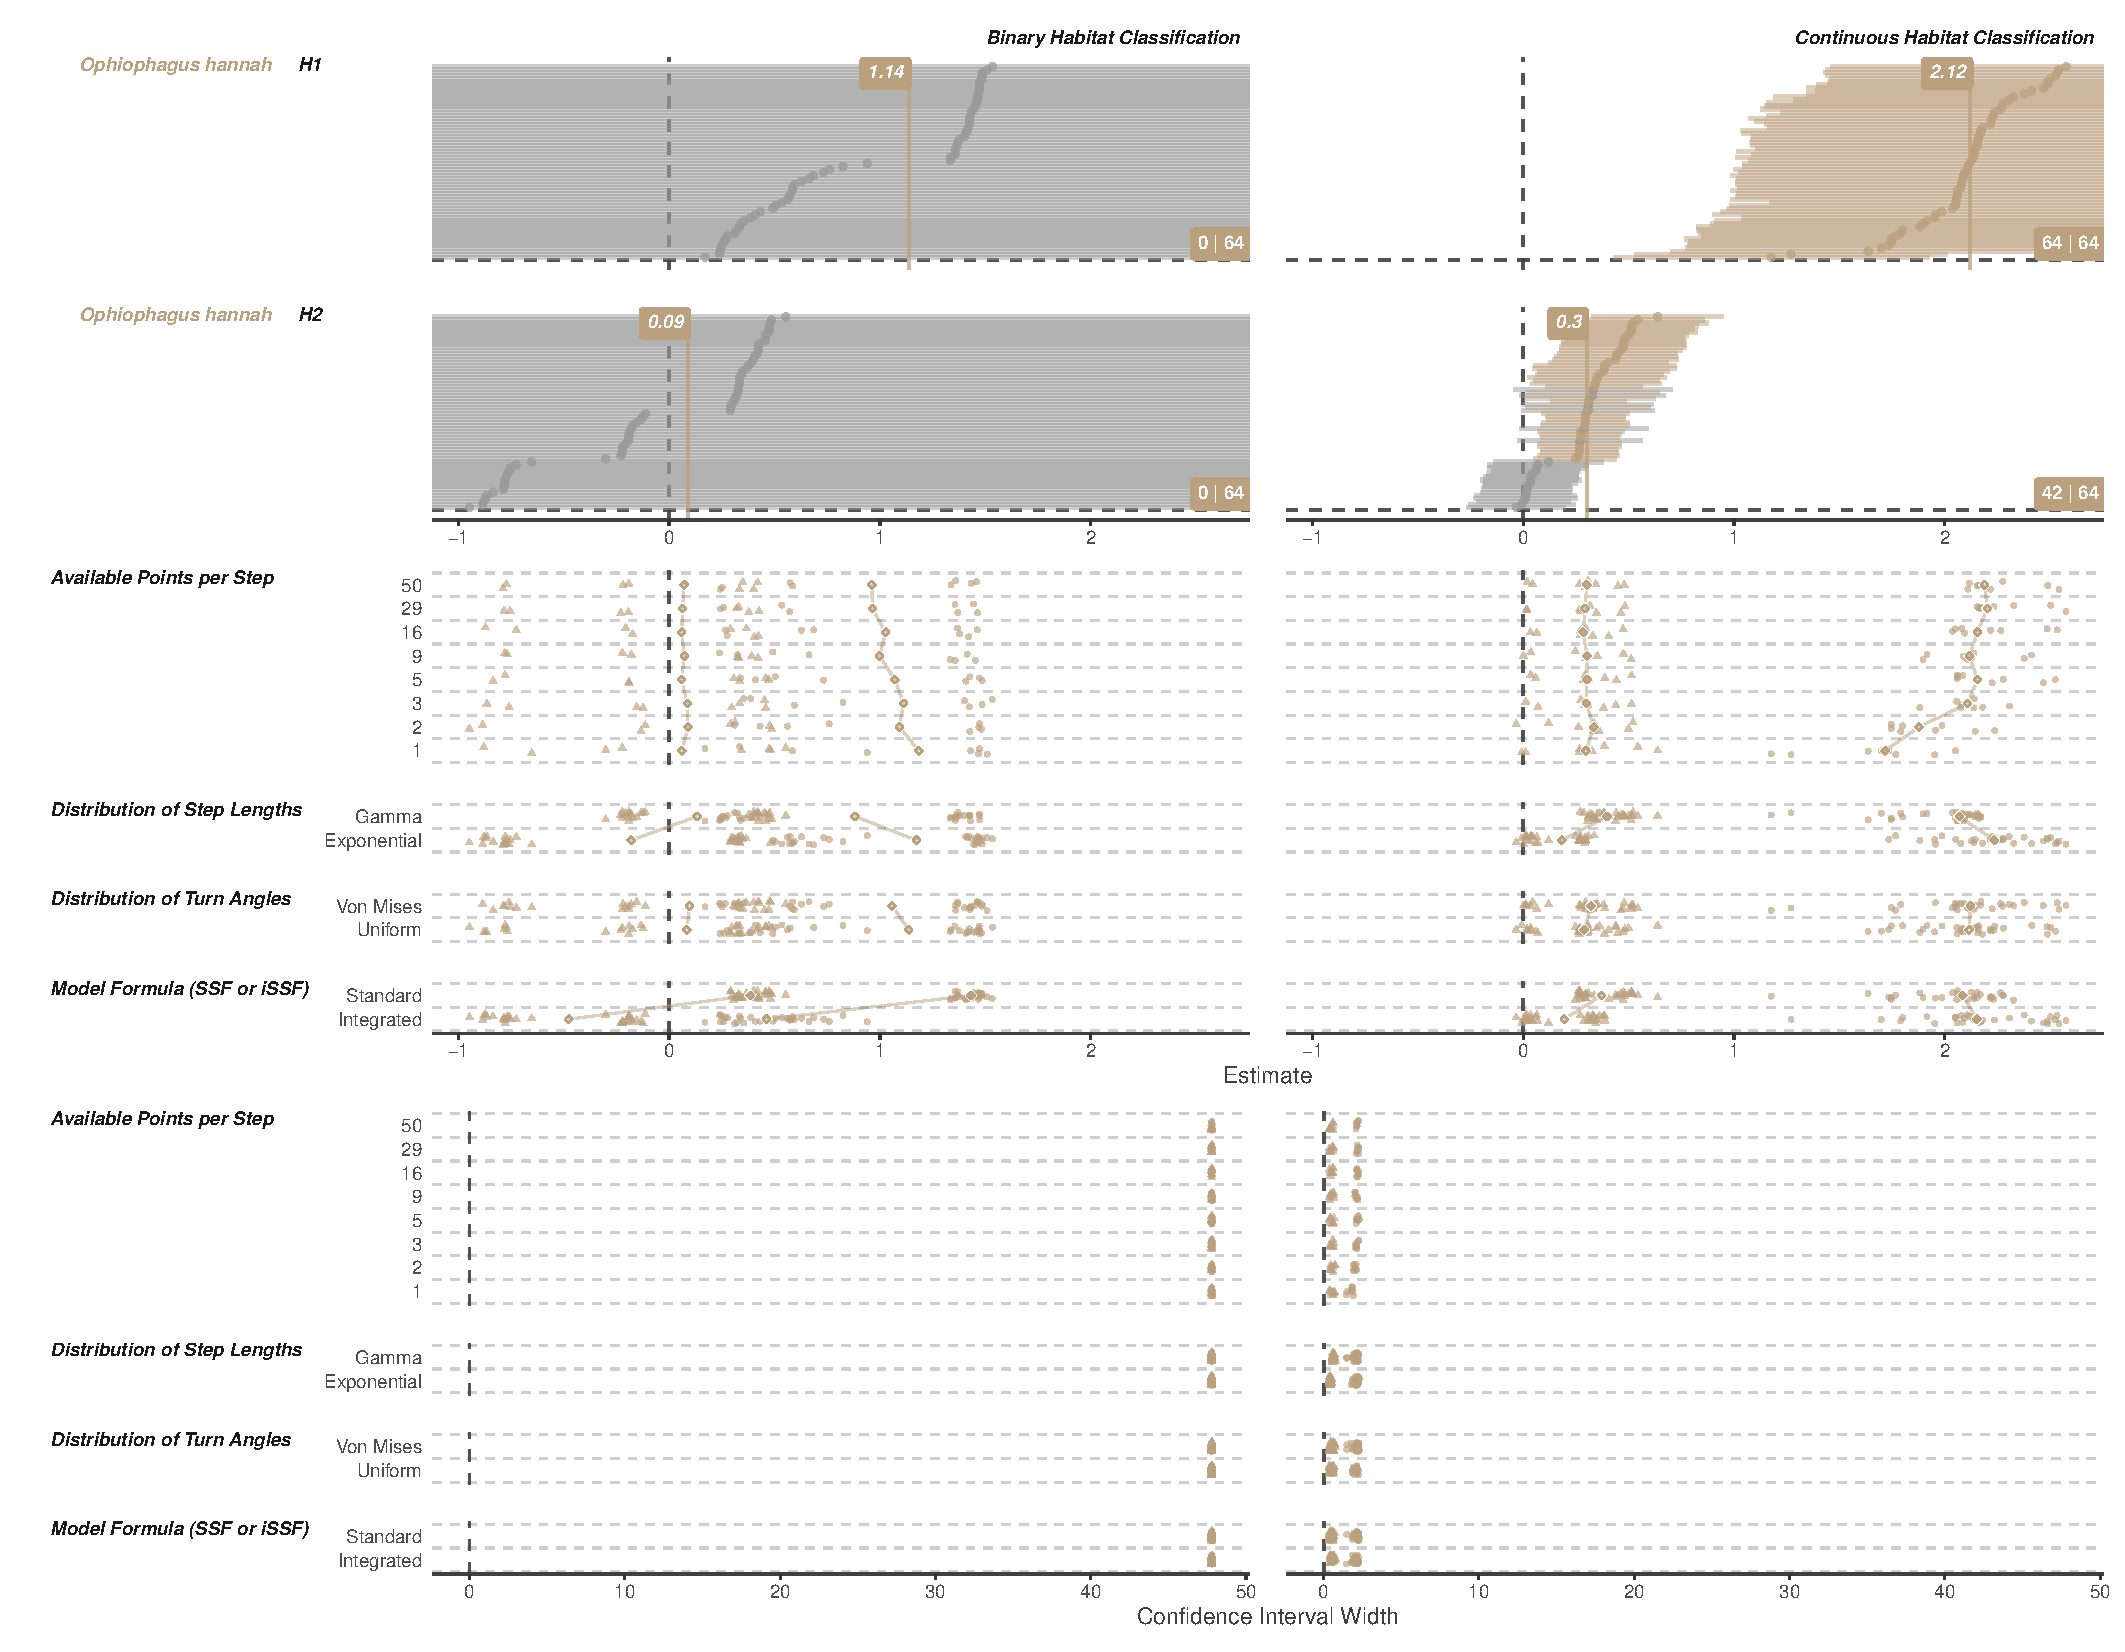
\includegraphics[width=1\linewidth]{../../figures/specCurve_Ophiophagus hannah_pois} \caption{All estimates of habitat selection derived from the step-based Poisson model (Poisson) analysis for King Cobras (Ophiophagus hannah). Top curves show all estimates, split by hypothesis, with coloured points and corresponding confidence intervals indicating whether those estimates significantly support the hypothesis. Bottom right labels provide a count of estimates that significantly support the hypothesis out of the total estimates. Labelled vertical lines show the median point estimate for each hypothesis. Lower plot show the estimates relative to each analysis choice. Shape separate hypothesis 1 and 2 (circles = hypothesis 1, triangle = hypothesis 2). Median estimates are shown with hollow diamonds, and hypothesis medians are connected with appropriated coloured lines. The plot is split left and right for the analysis using a binary classification (left), and continuous inverted distance (right).}\label{fig:specCurvePoisOPHA}
\end{figure}

\subsubsection{\texorpdfstring{Burmese Pythons (\emph{Python bivittatus})}{Burmese Pythons (Python bivittatus)}}\label{burmese-pythons-python-bivittatus}

\begin{figure}
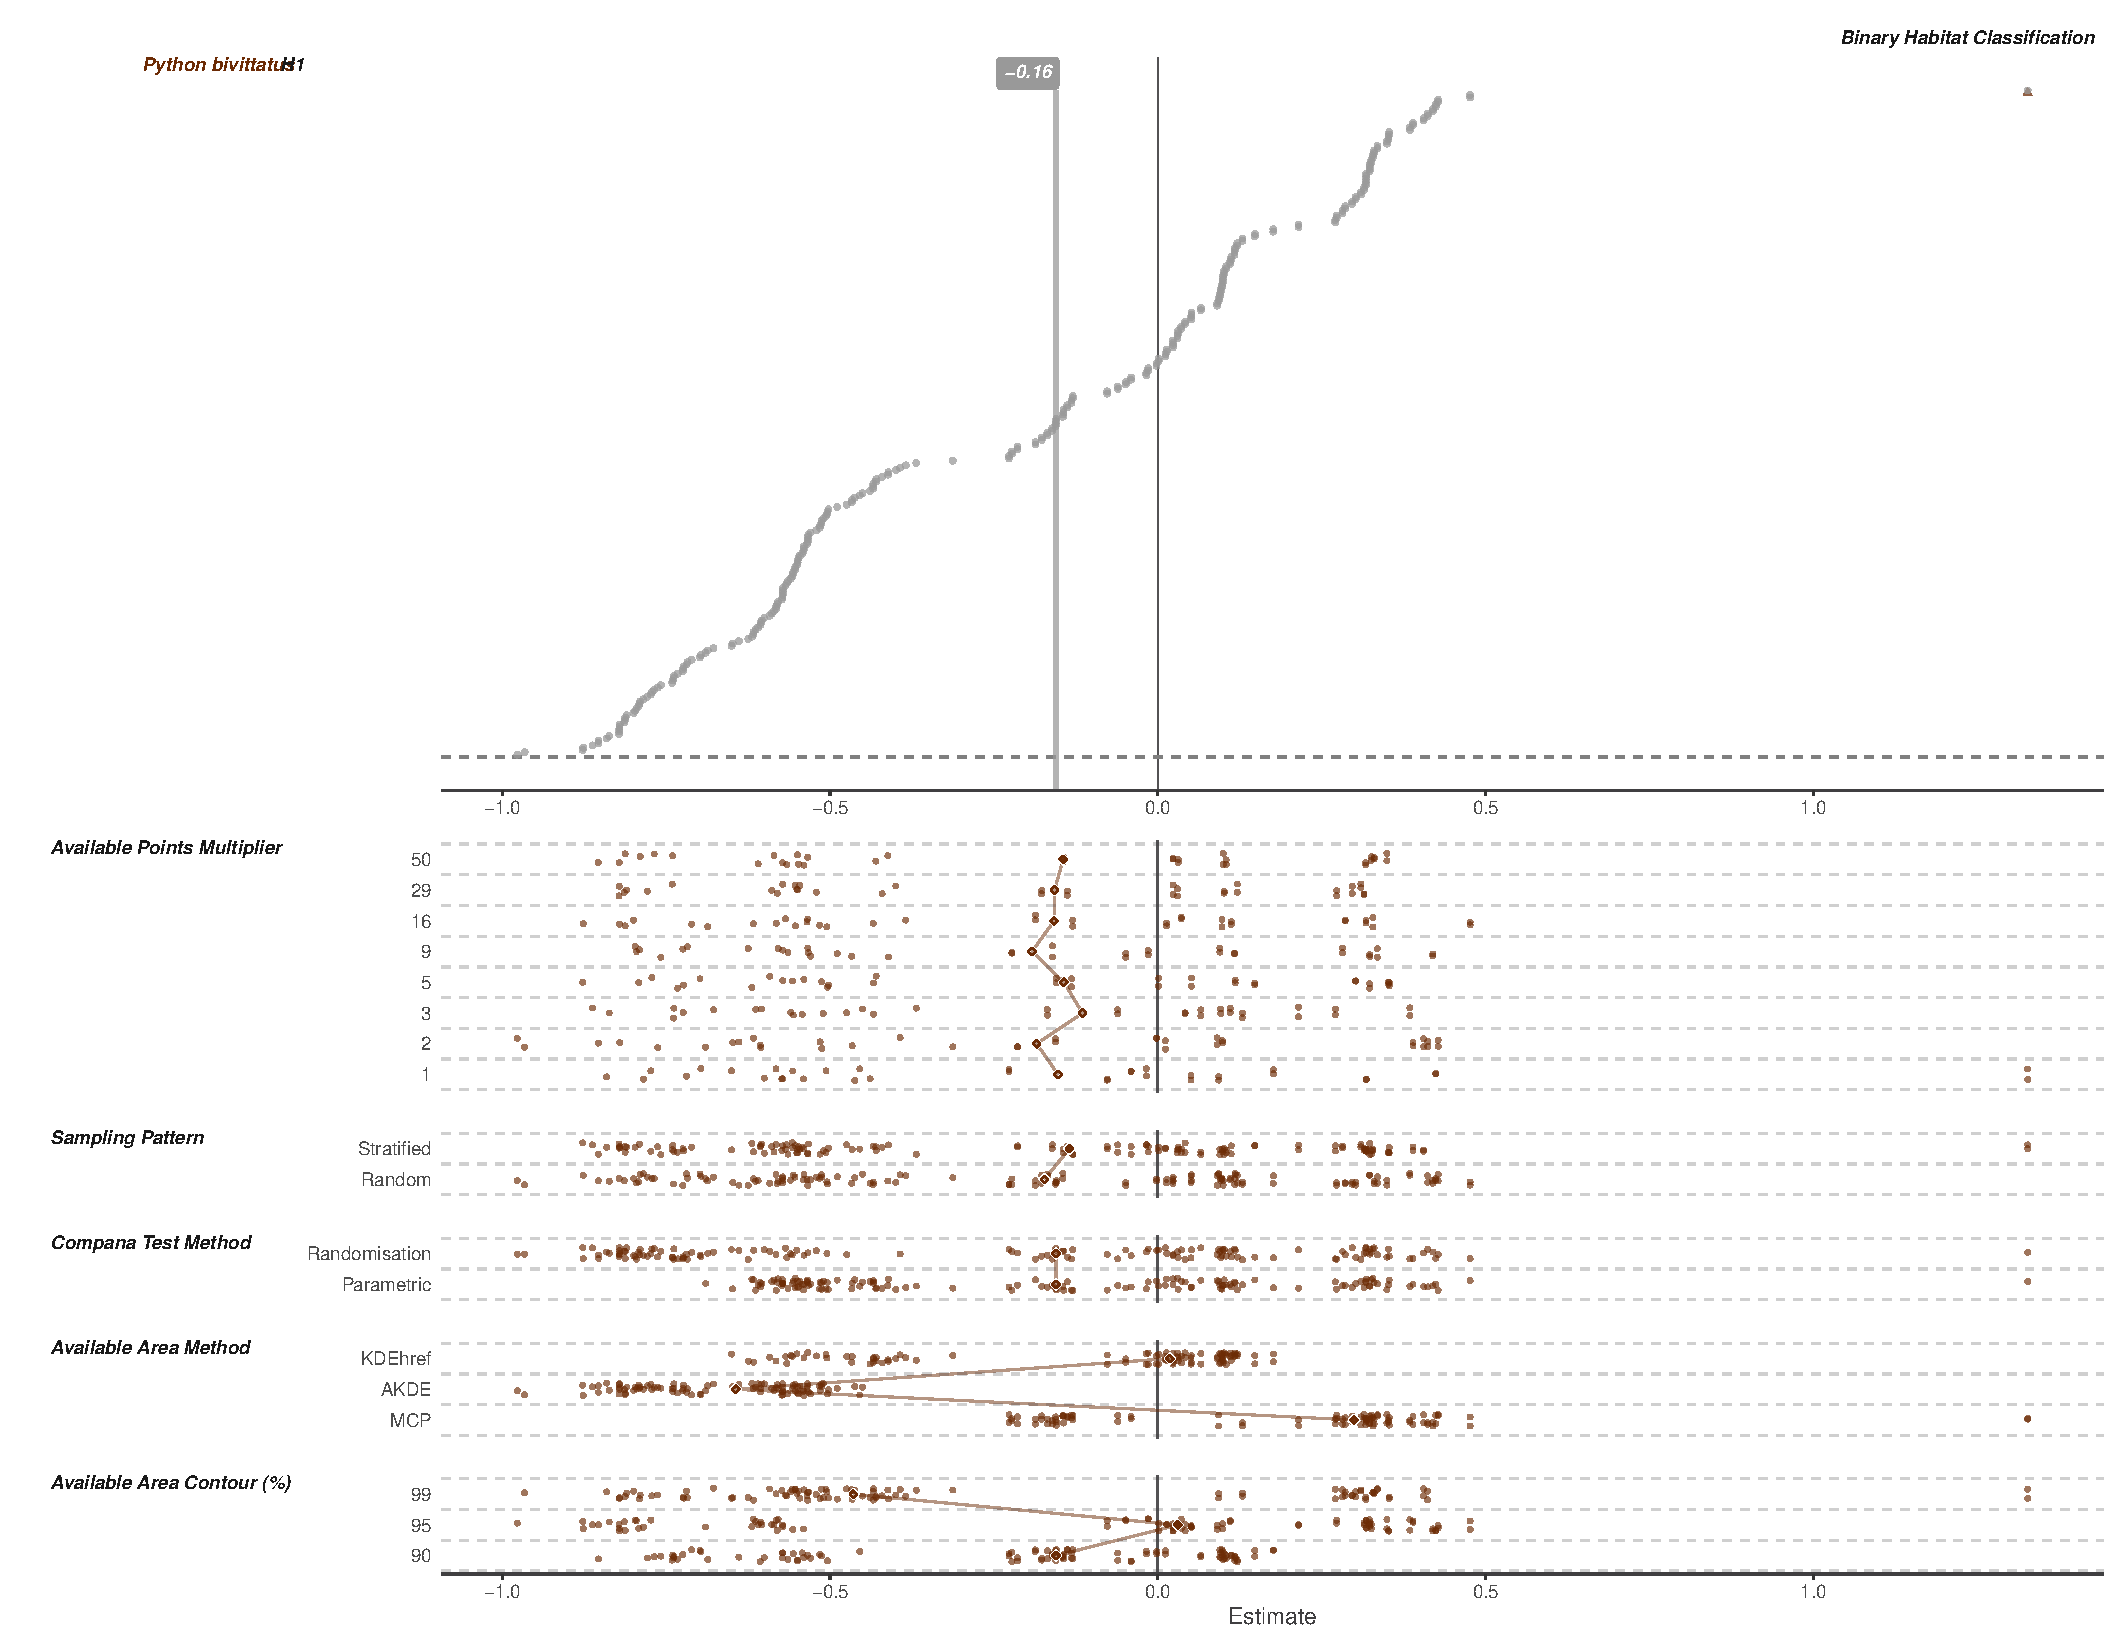
\includegraphics[width=1\linewidth]{../../figures/specCurve_Python bivittatus_area} \caption{All estimates of habitat selection derived from the areas-based Compositional (Compana) analysis for Banded Kraits (Python bivittatus). Top curves show all estimates with coloured points and corresponding confidence intervals indicating whether those estimates significantly support the hypothesis. Bottom right labels provide a count of estimates that significantly support the hypothesis out of the total estimates. Labelled vertical lines show the median point estimate. Lower plot show the estimates relative to each analysis choice. Median estimates are shown with hollow diamonds, and are connected with appropriated coloured lines.}\label{fig:specCurveAreaPYBI}
\end{figure}

\begin{figure}
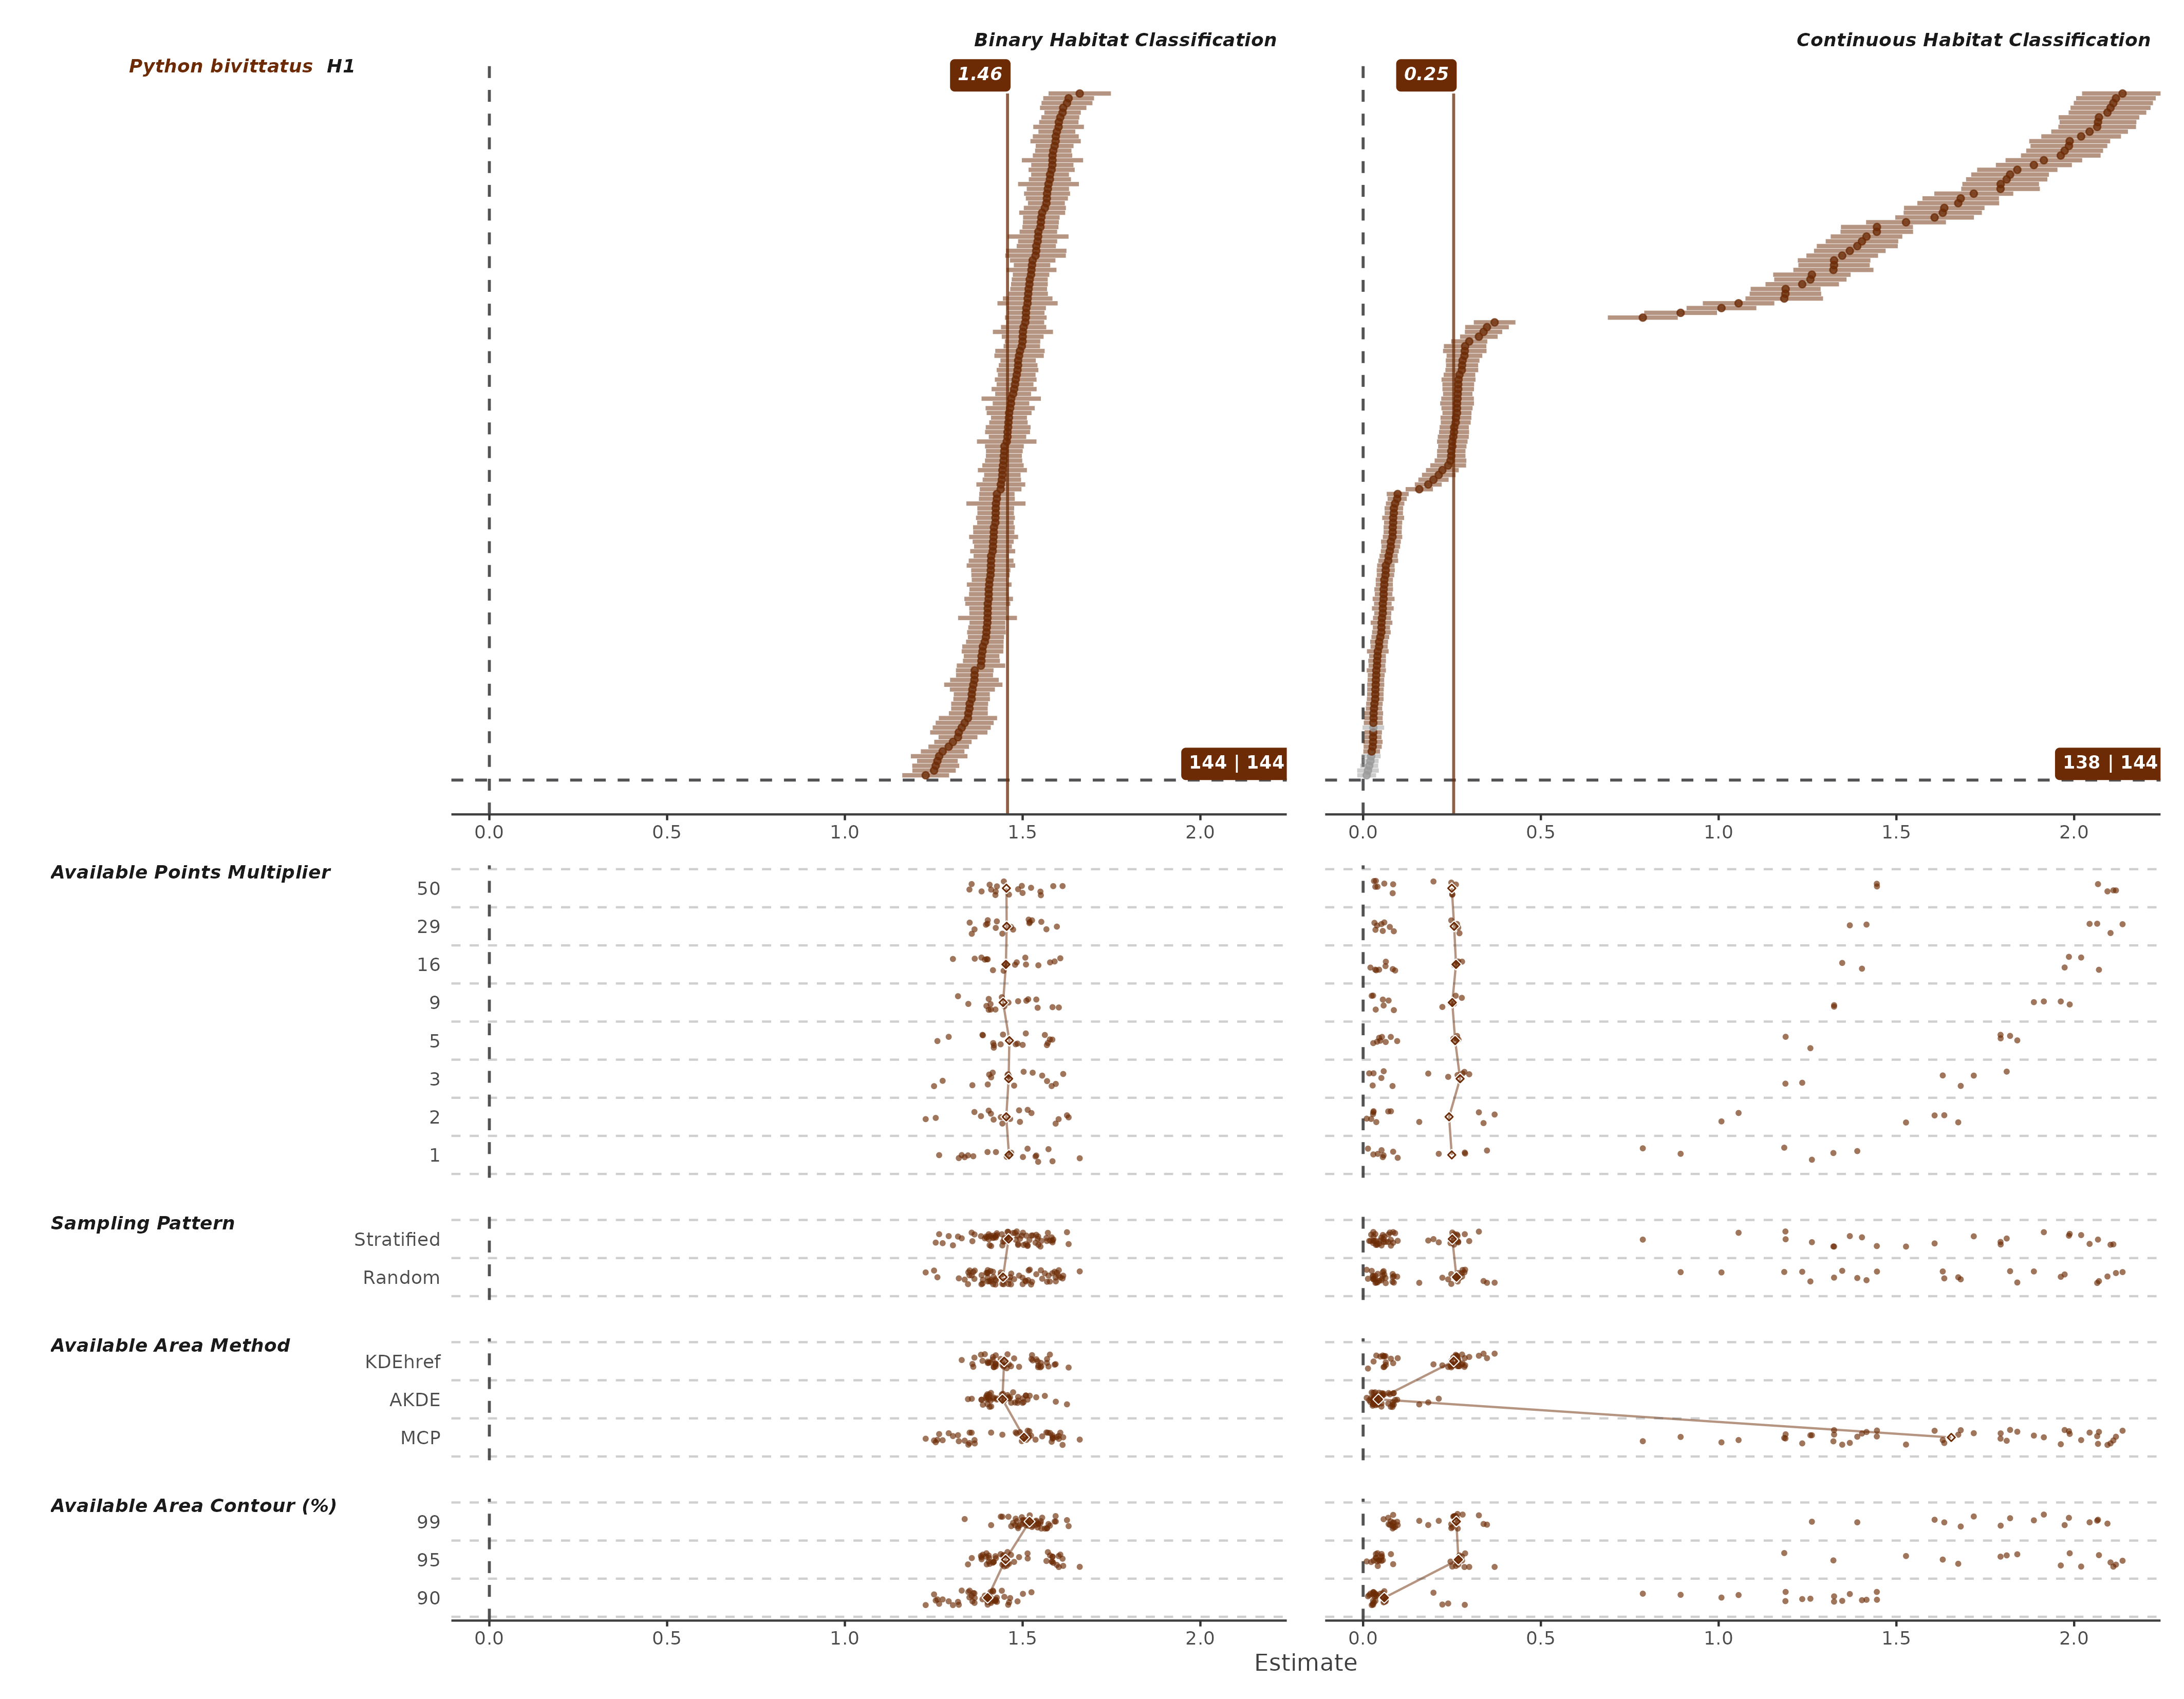
\includegraphics[width=1\linewidth]{../../figures/specCurve_Python bivittatus_rsf} \caption{All estimates of habitat selection derived from the areas-based Resource Selection Function (RSF) analysis for Banded Kraits (Python bivittatus). Top curves show all estimates with coloured points and corresponding confidence intervals indicating whether those estimates significantly support the hypothesis. Bottom right labels provide a count of estimates that significantly support the hypothesis out of the total estimates. Labelled vertical lines show the median point estimate. Lower plot show the estimates relative to each analysis choice. Median estimates are shown with hollow diamonds, and are connected with appropriated coloured lines. The plot is split left and right for the analysis using a binary classification (left), and continuous inverted distance (right).}\label{fig:specCurveRsfPYBI}
\end{figure}

\begin{figure}
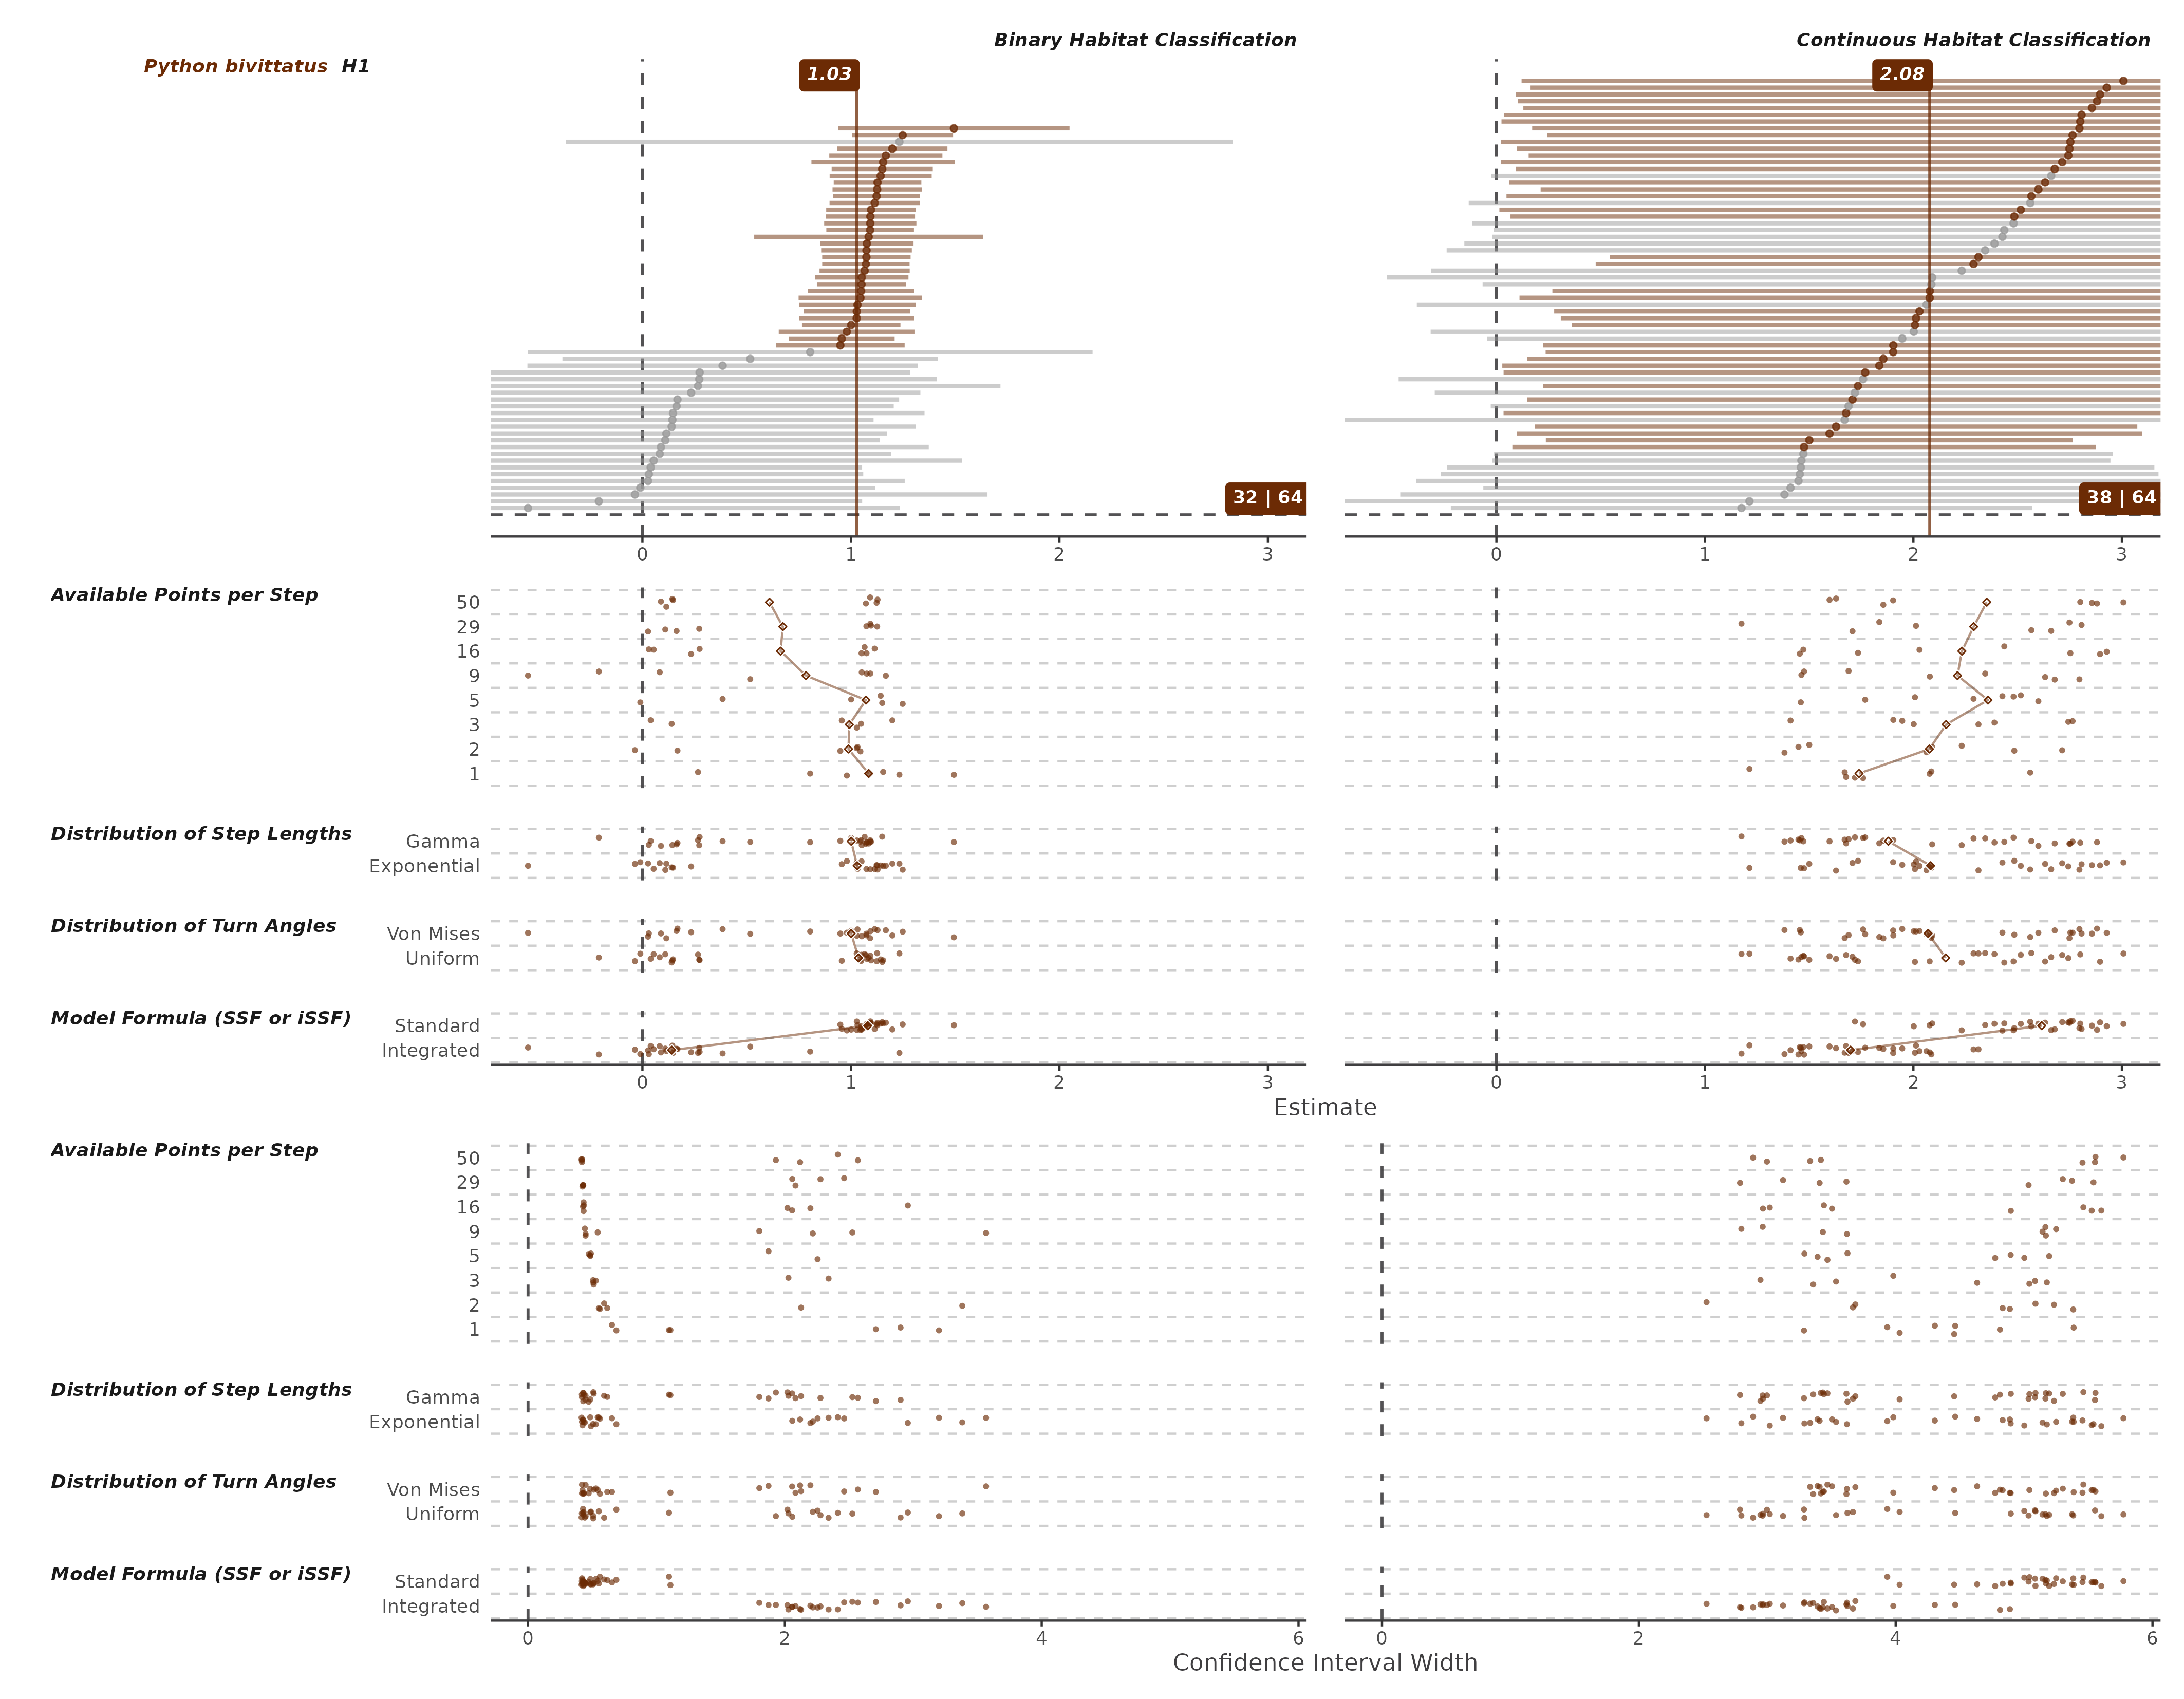
\includegraphics[width=1\linewidth]{../../figures/specCurve_Python bivittatus_twoStep} \caption{All estimates of habitat selection derived from the step-based Two-Step analysis for Banded Kraits (Python bivittatus). Top curves show all estimates with coloured points and corresponding confidence intervals indicating whether those estimates significantly support the hypothesis. Bottom right labels provide a count of estimates that significantly support the hypothesis out of the total estimates. Labelled vertical lines show the median point estimate. Lower plot show the estimates relative to each analysis choice. Median estimates are shown with hollow diamonds, and are connected with appropriated coloured lines. The plot is split left and right for the analysis using a binary classification (left), and continuous inverted distance (right).}\label{fig:specCurveTwoStepPYBI}
\end{figure}

\begin{figure}
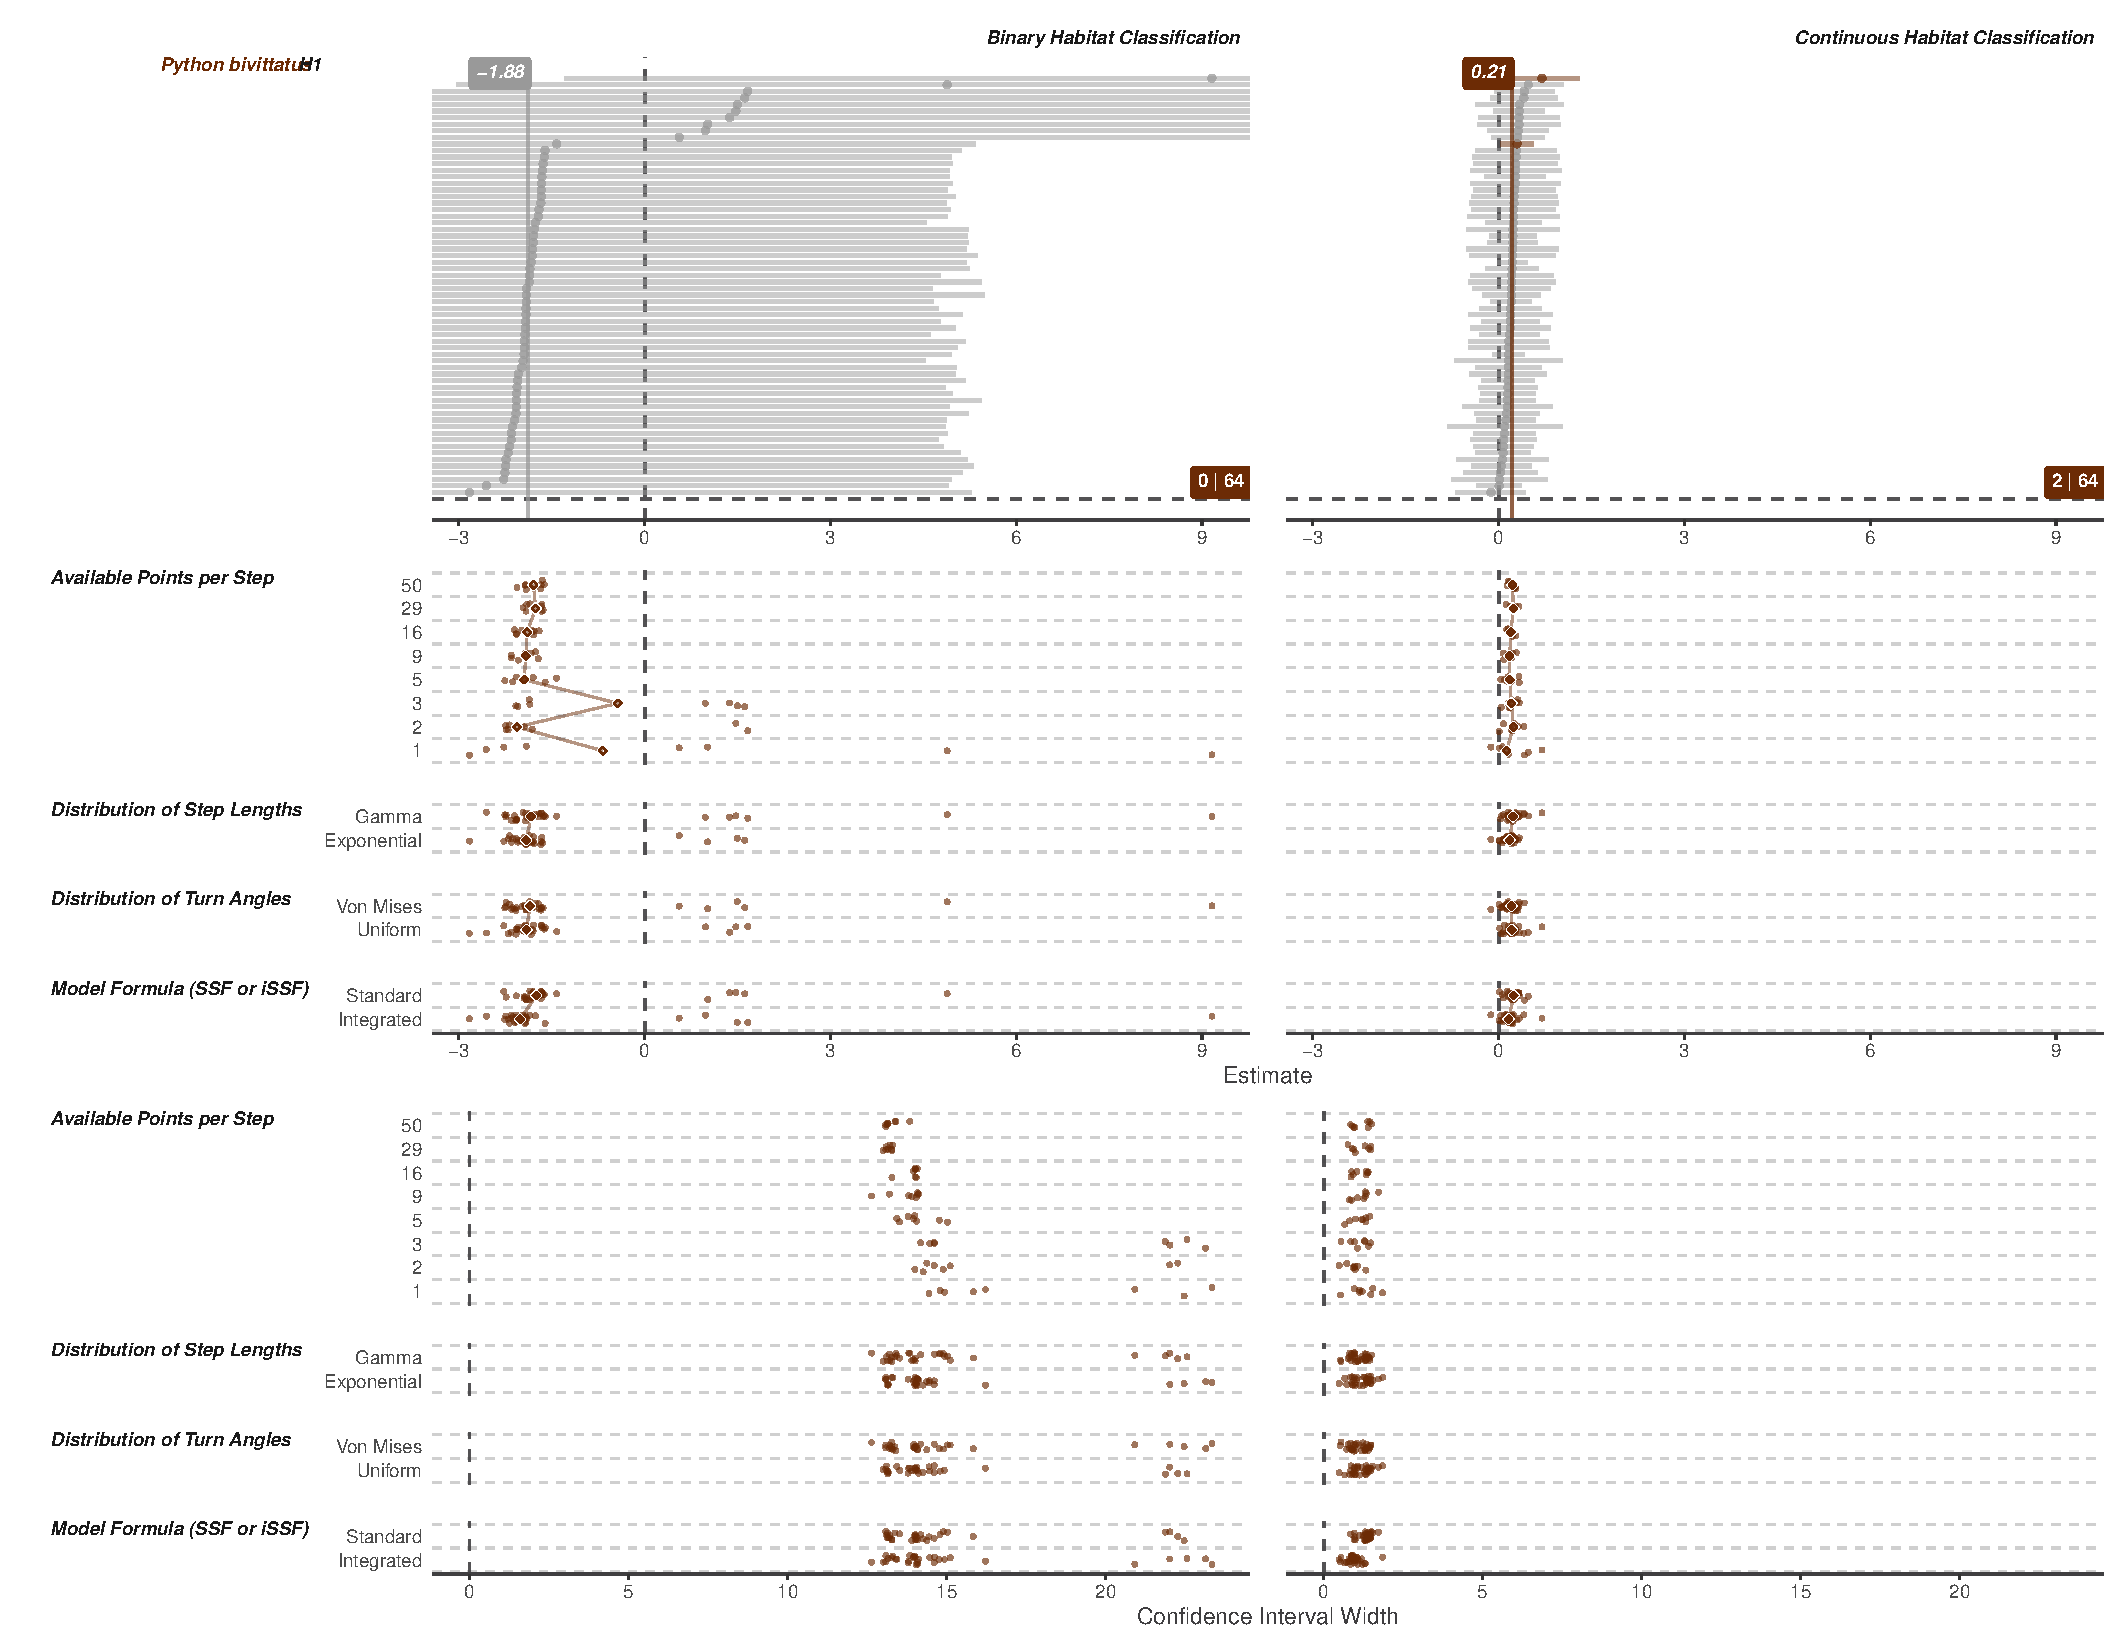
\includegraphics[width=1\linewidth]{../../figures/specCurve_Python bivittatus_ssf} \caption{All estimates of habitat selection derived from the step-based Step Selection Function (SSF) analysis for Banded Kraits (Python bivittatus). Top curves show all estimates with coloured points and corresponding confidence intervals indicating whether those estimates significantly support the hypothesis. Bottom right labels provide a count of estimates that significantly support the hypothesis out of the total estimates. Labelled vertical lines show the median point estimate. Lower plot show the estimates relative to each analysis choice. Median estimates are shown with hollow diamonds, and are connected with appropriated coloured lines. The plot is split left and right for the analysis using a binary classification (left), and continuous inverted distance (right).}\label{fig:specCurveSsfPYBI}
\end{figure}

\begin{figure}
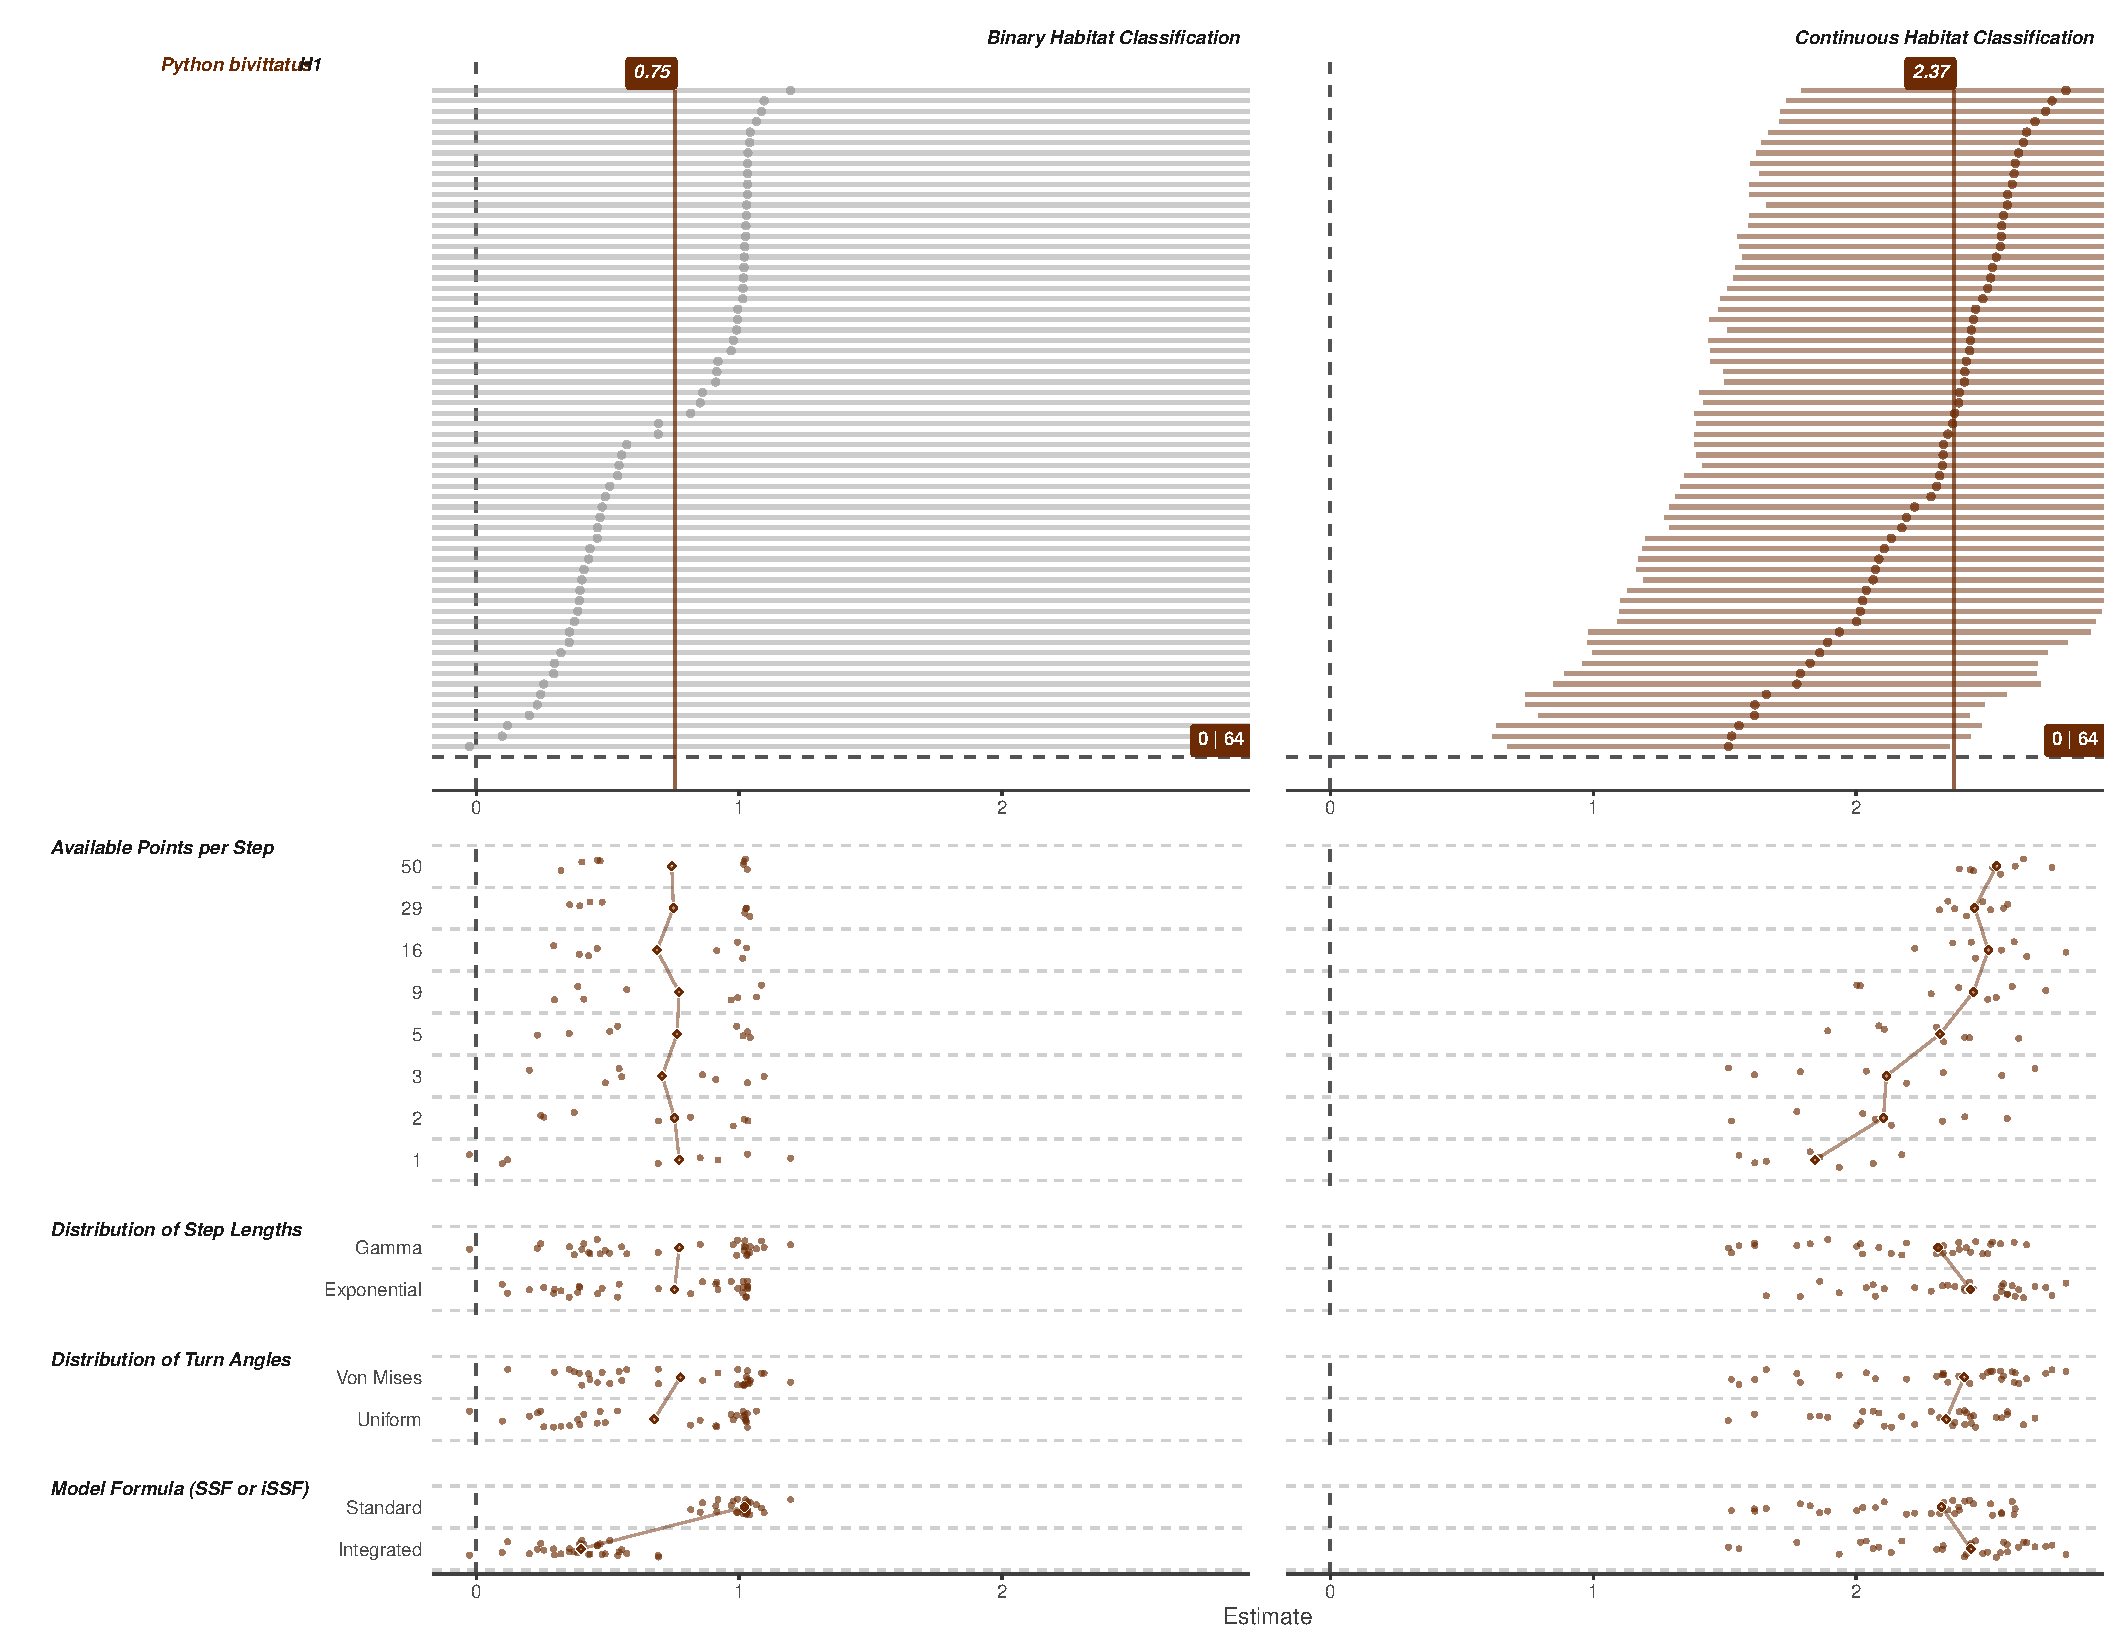
\includegraphics[width=1\linewidth]{../../figures/specCurve_Python bivittatus_pois} \caption{All estimates of habitat selection derived from the step-based Poisson model (Poisson) analysis for Banded Kraits (Python bivittatus). Top curves show all estimates with coloured points and corresponding confidence intervals indicating whether those estimates significantly support the hypothesis. Bottom right labels provide a count of estimates that significantly support the hypothesis out of the total estimates. Labelled vertical lines show the median point estimate. Lower plot show the estimates relative to each analysis choice. Median estimates are shown with hollow diamonds, and are connected with appropriated coloured lines. The plot is split left and right for the analysis using a binary classification (left), and continuous inverted distance (right).}\label{fig:specCurvePoisPYBI}
\end{figure}

\subsubsection{\texorpdfstring{Malayan Kraits (\emph{Bungarus candidus})}{Malayan Kraits (Bungarus candidus)}}\label{malayan-kraits-bungarus-candidus}

\begin{figure}
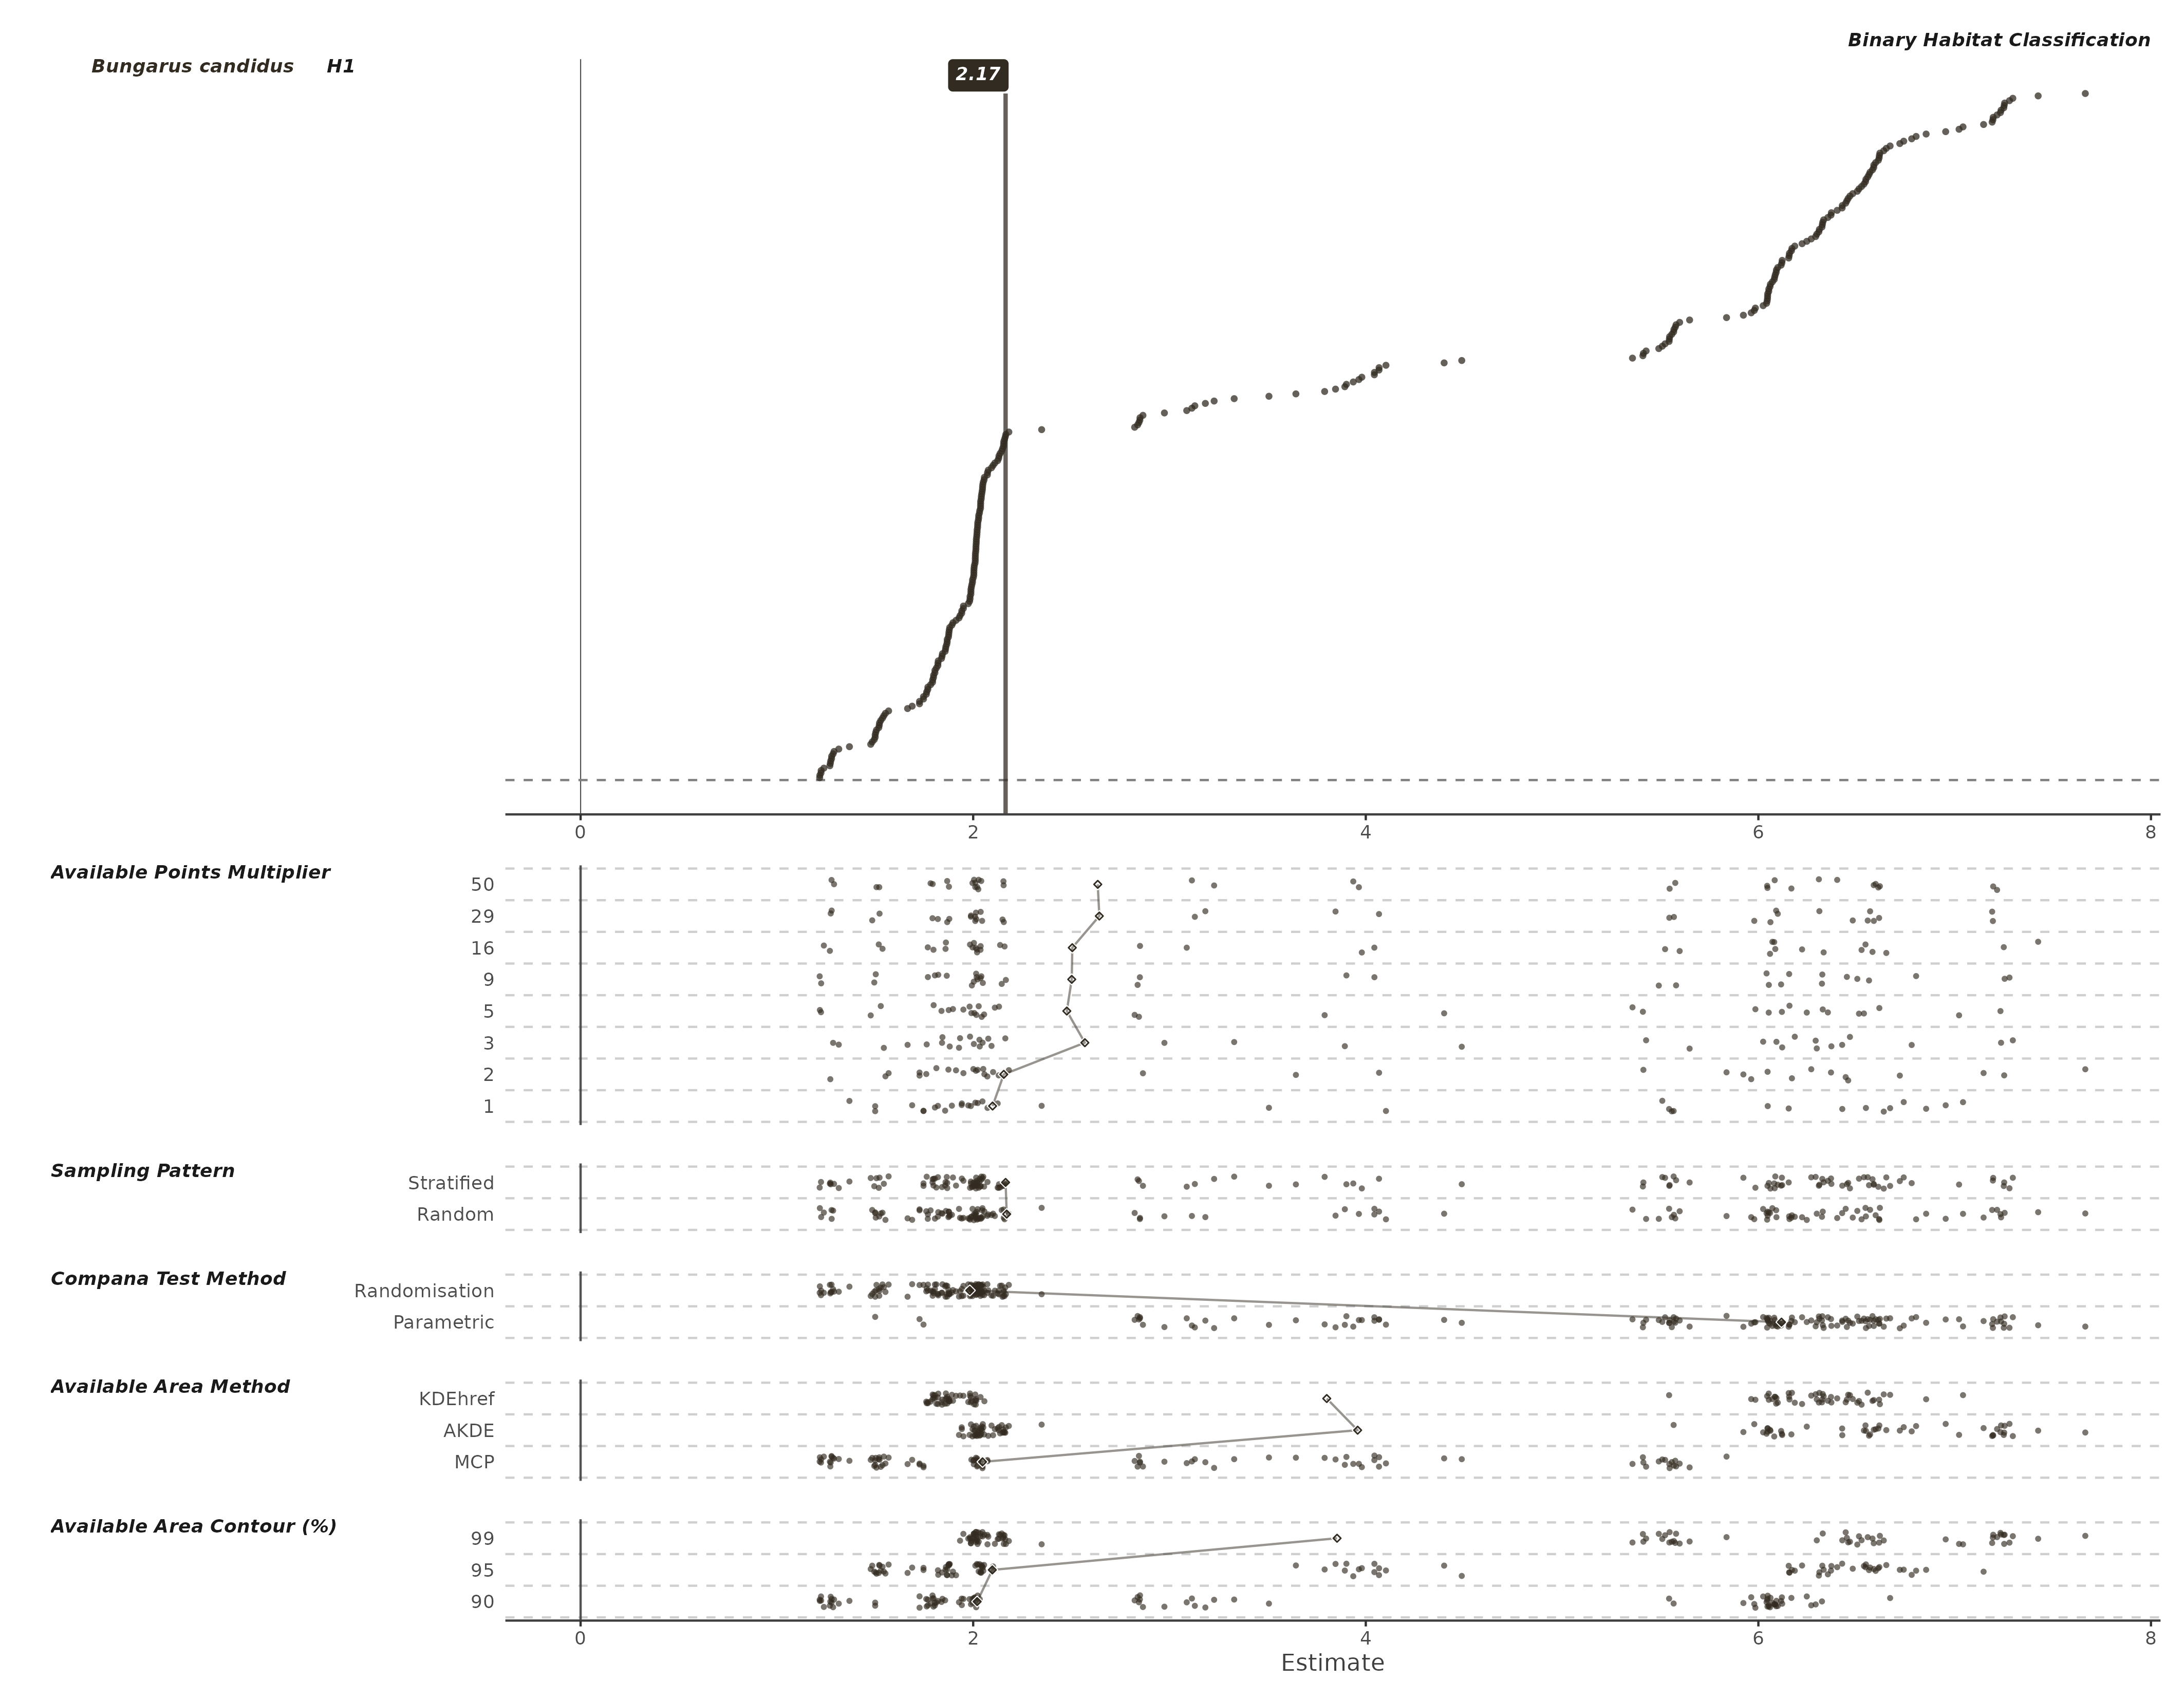
\includegraphics[width=1\linewidth]{../../figures/specCurve_Bungarus candidus_area} \caption{All estimates of habitat selection derived from the areas-based Compositional (Compana) analysis for Malayan Kraits (Bungarus candidus). Top curves show all estimates with coloured points and corresponding confidence intervals indicating whether those estimates significantly support the hypothesis. Bottom right labels provide a count of estimates that significantly support the hypothesis out of the total estimates. Labelled vertical lines show the median point estimate. Lower plot show the estimates relative to each analysis choice. Median estimates are shown with hollow diamonds, and are connected with appropriated coloured lines.}\label{fig:specCurveAreaBUCA}
\end{figure}

\begin{figure}
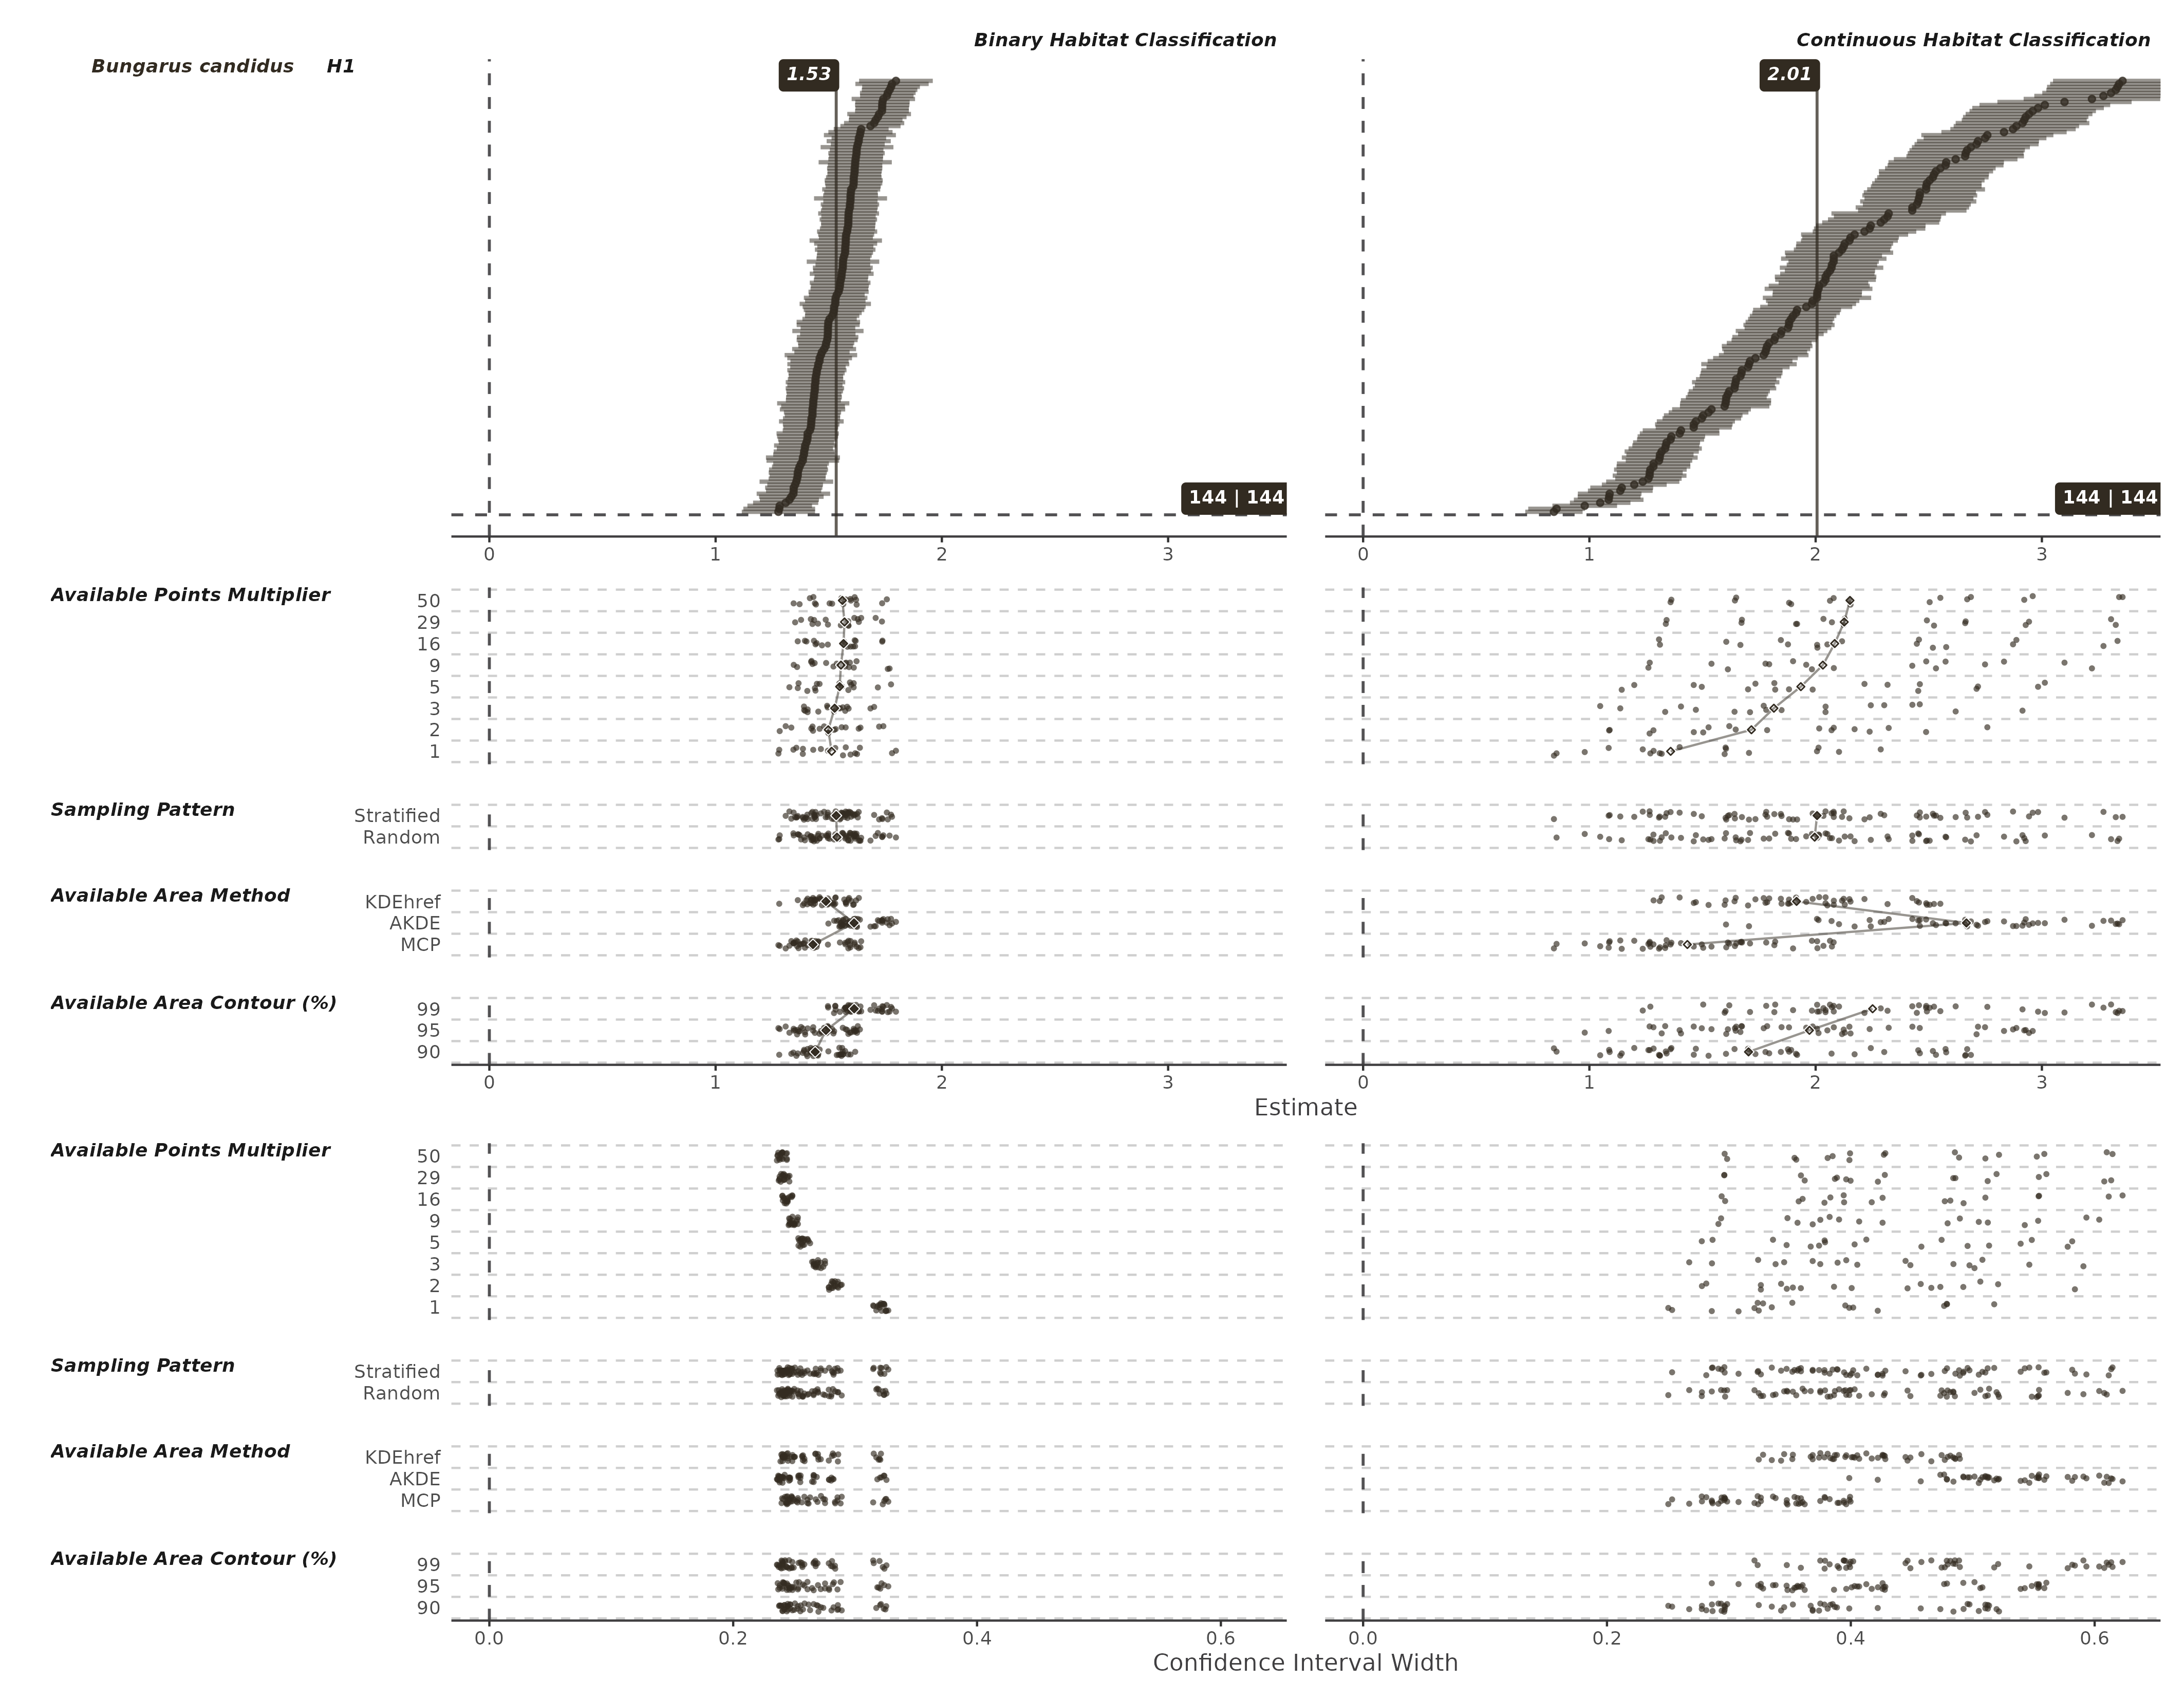
\includegraphics[width=1\linewidth]{../../figures/specCurve_Bungarus candidus_rsf} \caption{All estimates of habitat selection derived from the areas-based Resource Selection Function (RSF) analysis for Malayan Kraits (Bungarus candidus). Top curves show all estimates with coloured points and corresponding confidence intervals indicating whether those estimates significantly support the hypothesis. Bottom right labels provide a count of estimates that significantly support the hypothesis out of the total estimates. Labelled vertical lines show the median point estimate. Lower plot show the estimates relative to each analysis choice. Median estimates are shown with hollow diamonds, and are connected with appropriated coloured lines. The plot is split left and right for the analysis using a binary classification (left), and continuous inverted distance (right).}\label{fig:specCurveRsfBUCA}
\end{figure}

\begin{figure}
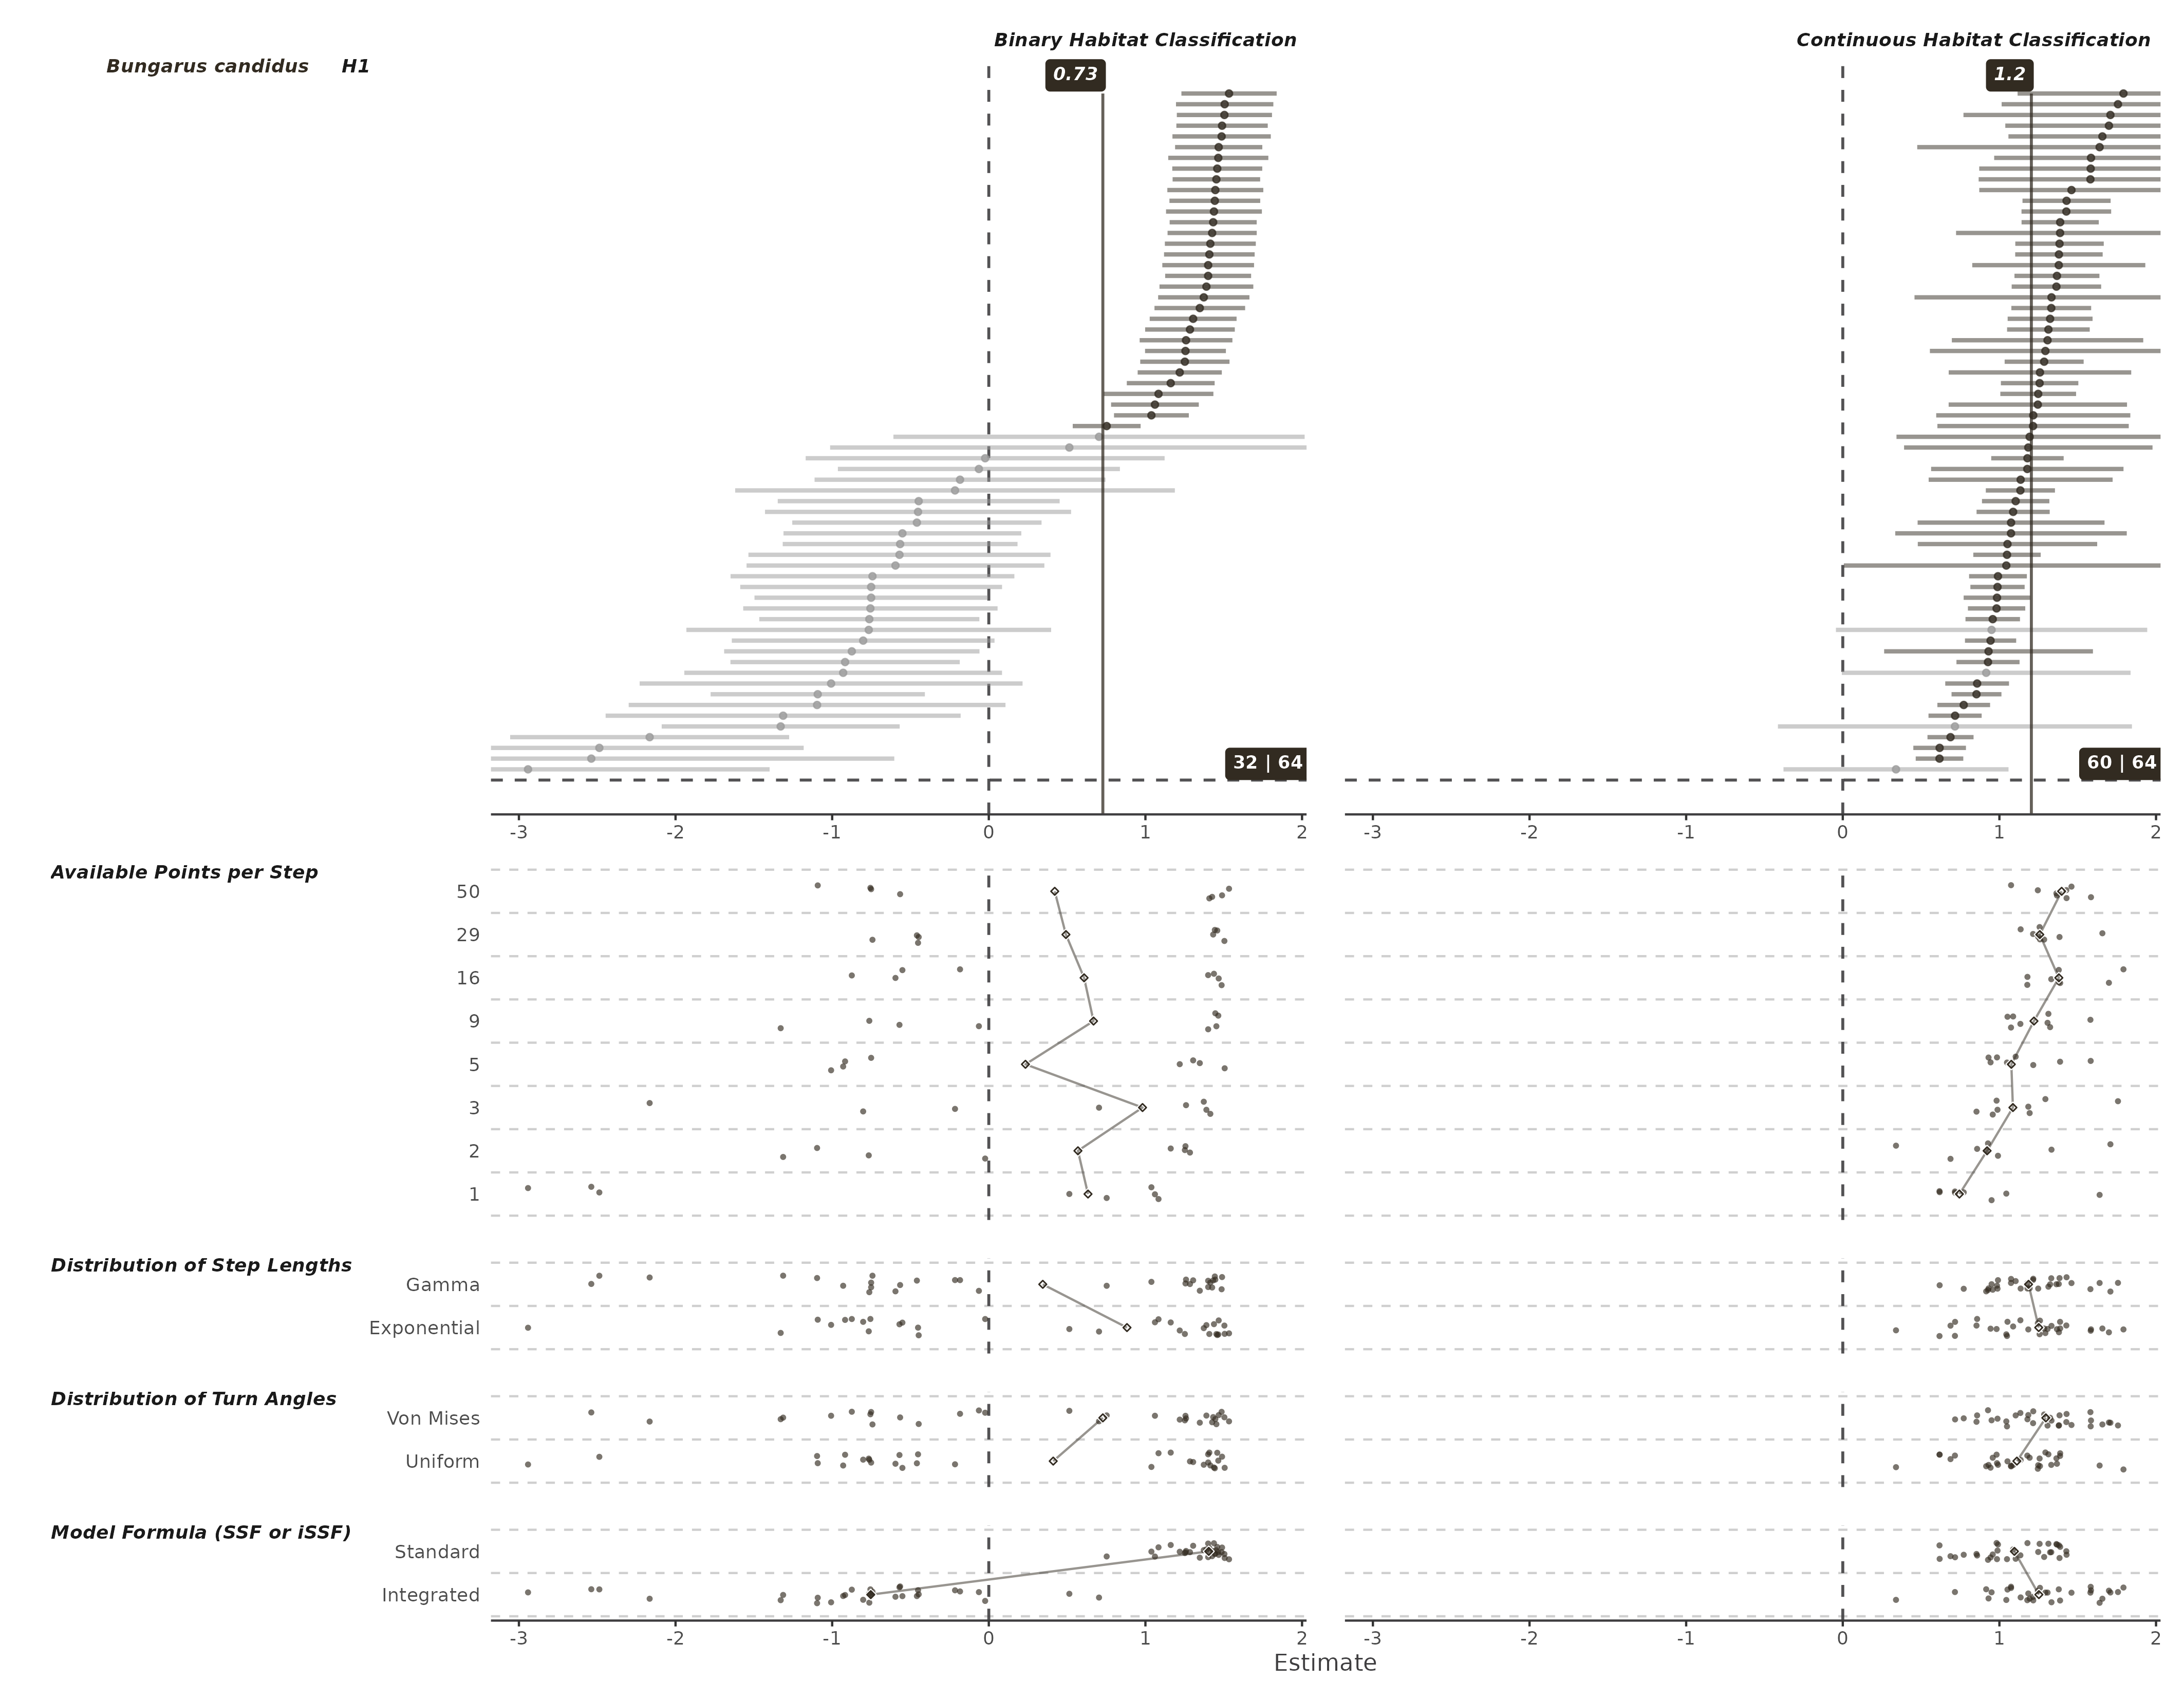
\includegraphics[width=1\linewidth]{../../figures/specCurve_Bungarus candidus_twoStep} \caption{All estimates of habitat selection derived from the step-based Two-Step analysis for Malayan Kraits (Bungarus candidus). Top curves show all estimates with coloured points and corresponding confidence intervals indicating whether those estimates significantly support the hypothesis. Bottom right labels provide a count of estimates that significantly support the hypothesis out of the total estimates. Labelled vertical lines show the median point estimate. Lower plot show the estimates relative to each analysis choice. Median estimates are shown with hollow diamonds, and are connected with appropriated coloured lines. The plot is split left and right for the analysis using a binary classification (left), and continuous inverted distance (right).}\label{fig:specCurveTwoStepBUCA}
\end{figure}

\begin{figure}
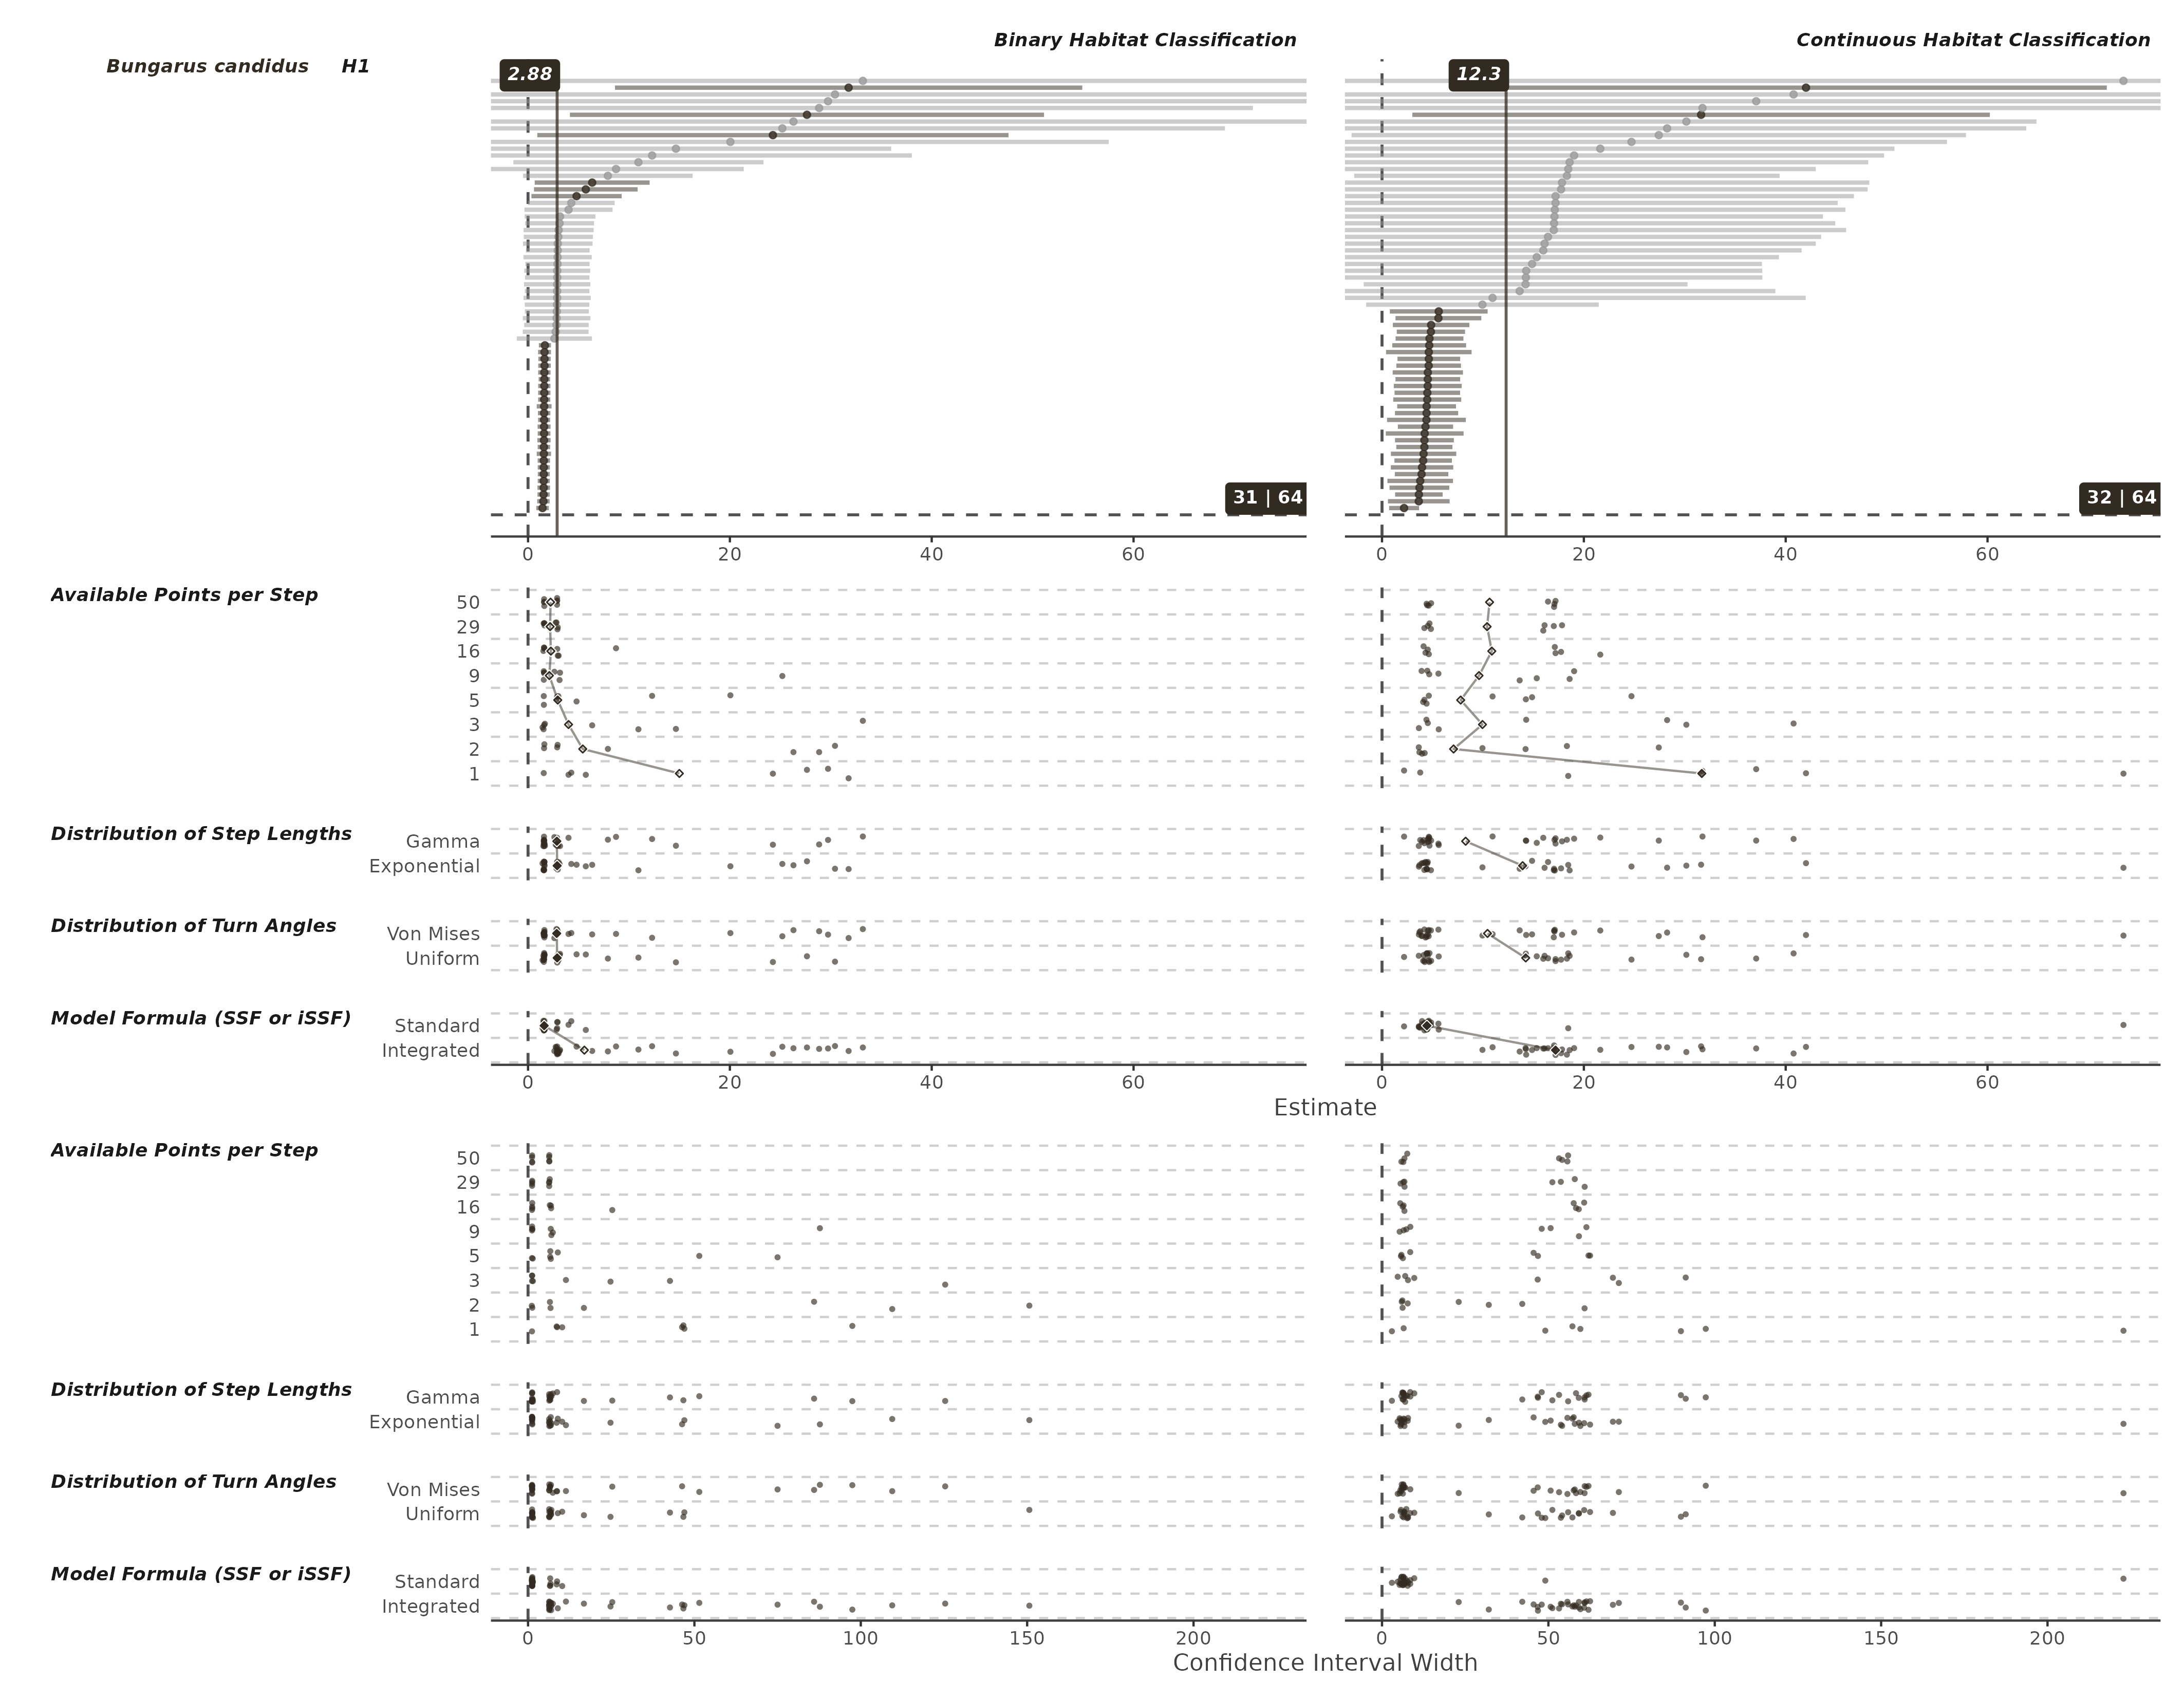
\includegraphics[width=1\linewidth]{../../figures/specCurve_Bungarus candidus_ssf} \caption{All estimates of habitat selection derived from the step-based Step Selection Function (SSF) analysis for Malayan Kraits (Bungarus candidus). Top curves show all estimates with coloured points and corresponding confidence intervals indicating whether those estimates significantly support the hypothesis. Bottom right labels provide a count of estimates that significantly support the hypothesis out of the total estimates. Labelled vertical lines show the median point estimate. Lower plot show the estimates relative to each analysis choice. Median estimates are shown with hollow diamonds, and are connected with appropriated coloured lines. The plot is split left and right for the analysis using a binary classification (left), and continuous inverted distance (right).}\label{fig:specCurveSsfBUCA}
\end{figure}

\begin{figure}
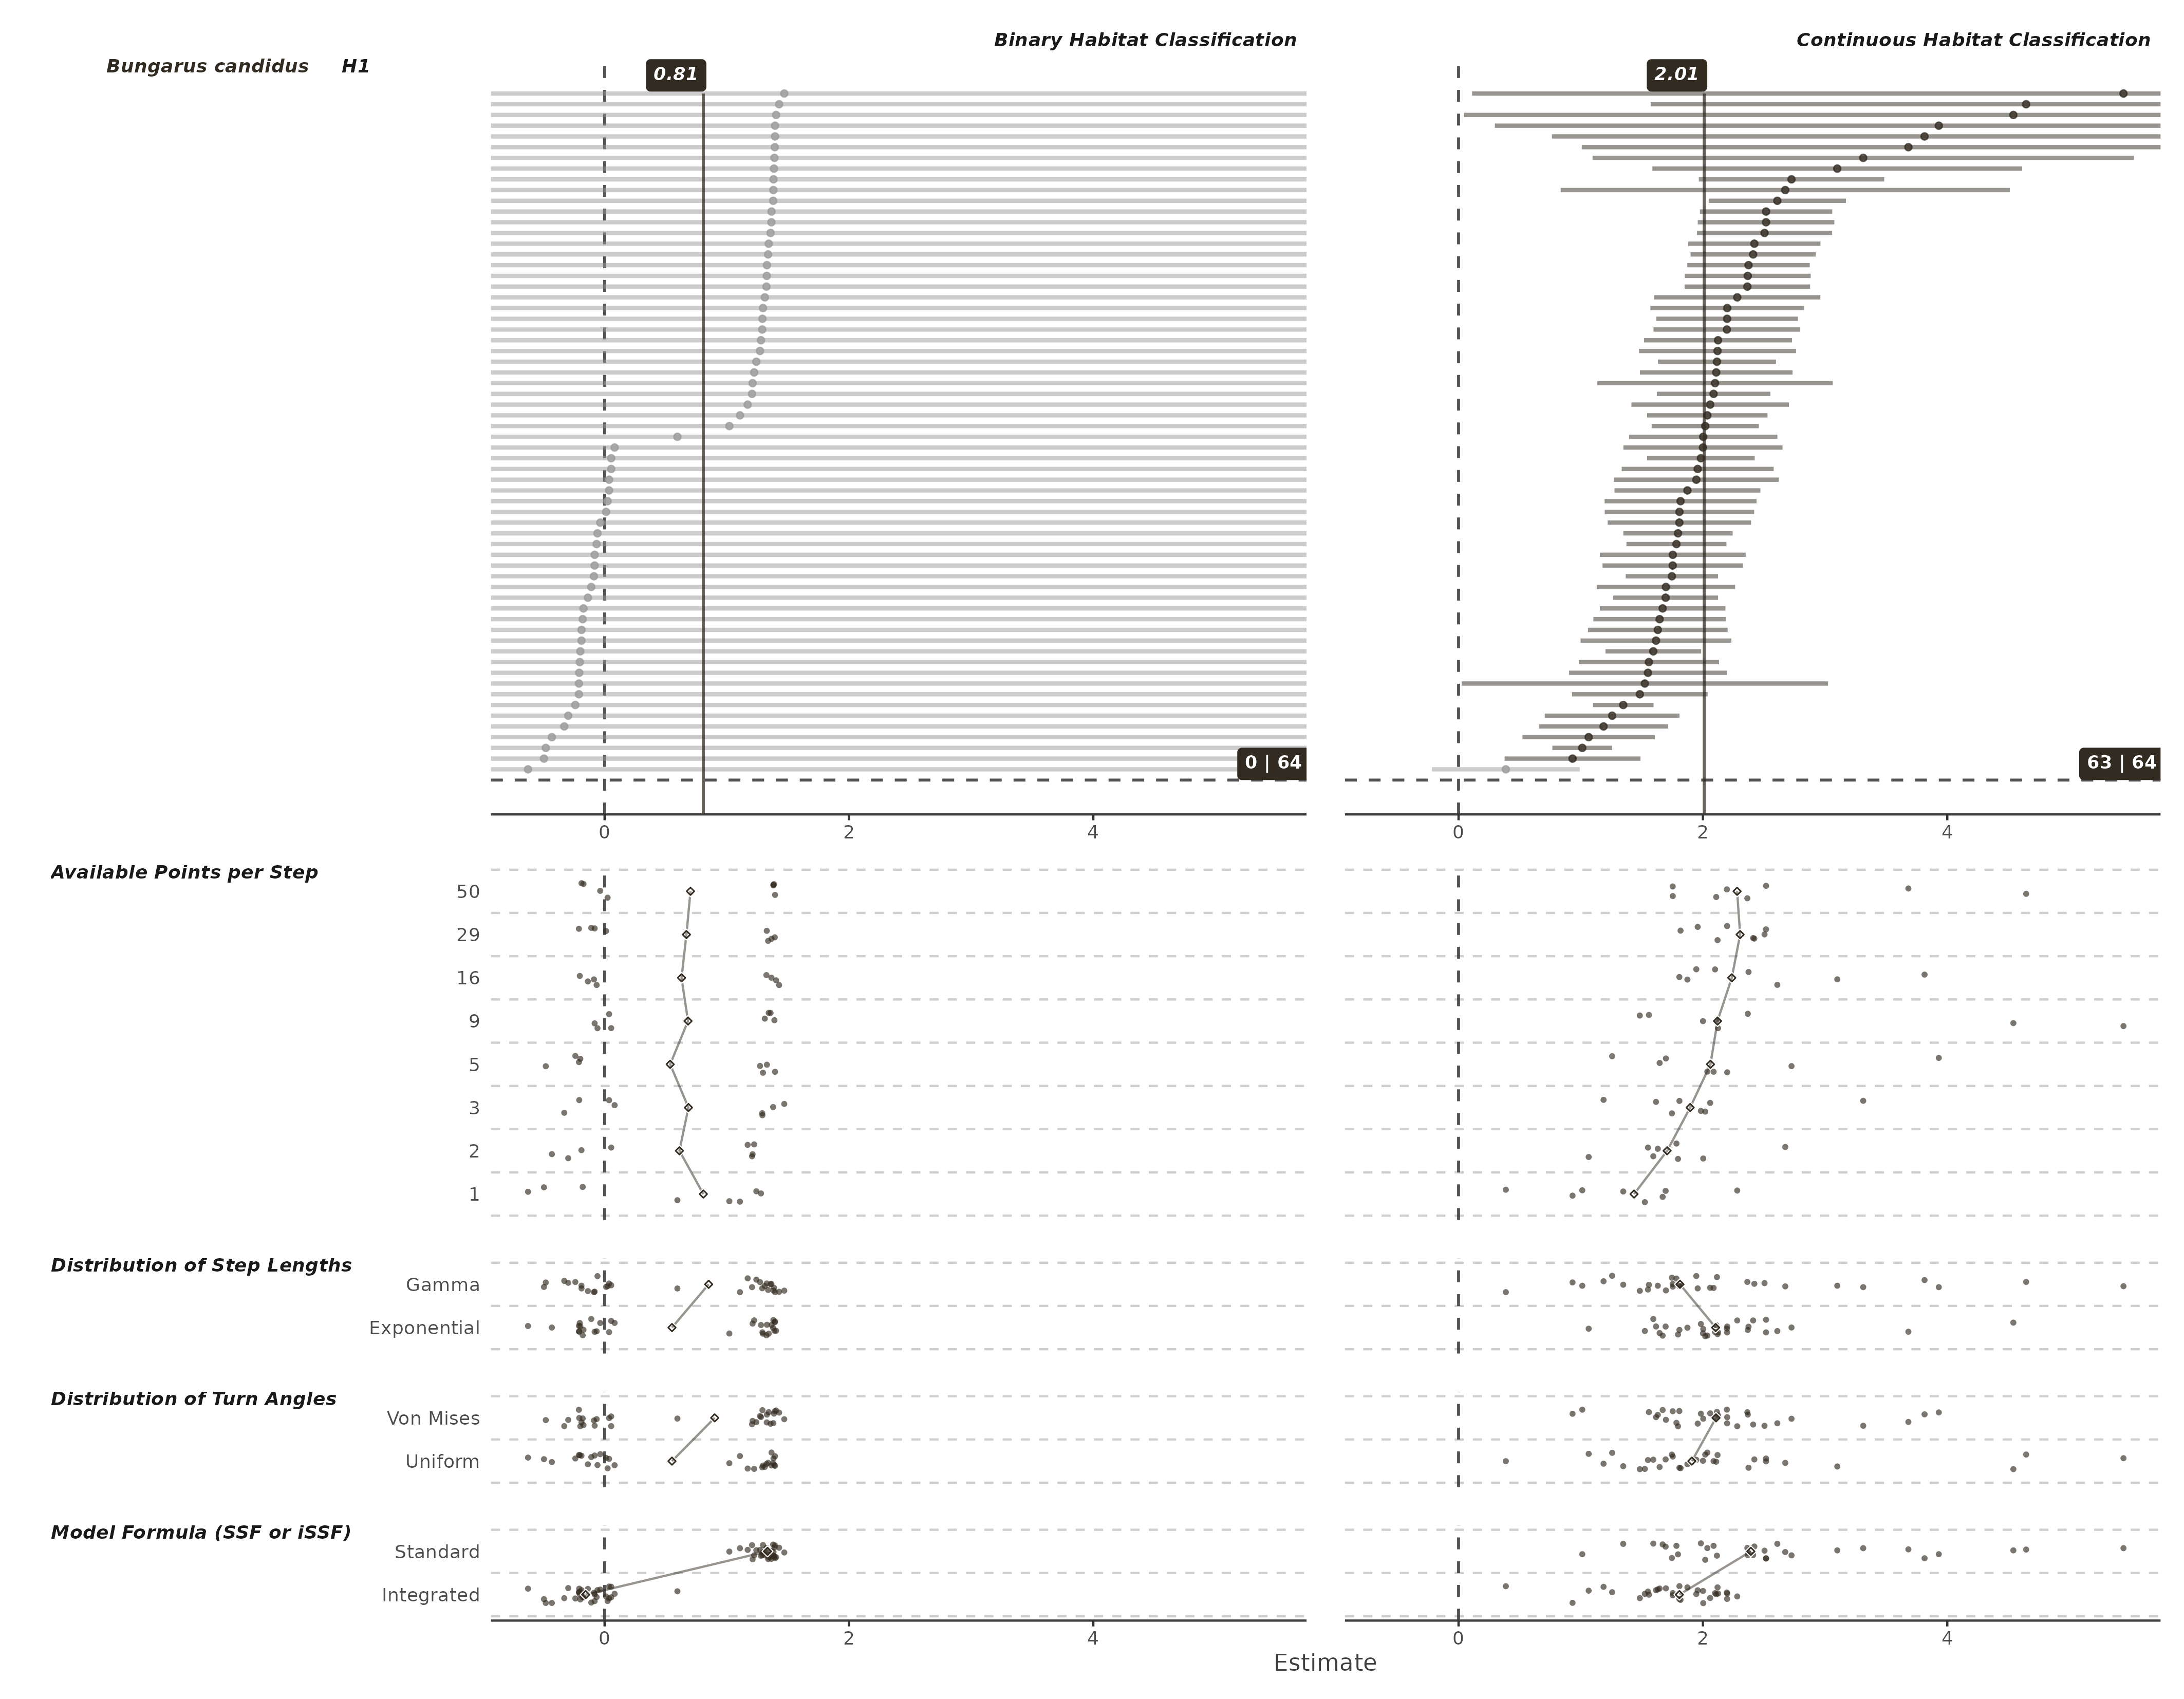
\includegraphics[width=1\linewidth]{../../figures/specCurve_Bungarus candidus_pois} \caption{All estimates of habitat selection derived from the step-based Poisson model (Poisson) analysis for Malayan Kraits (Bungarus candidus). Top curves show all estimates with coloured points and corresponding confidence intervals indicating whether those estimates significantly support the hypothesis. Bottom right labels provide a count of estimates that significantly support the hypothesis out of the total estimates. Labelled vertical lines show the median point estimate. Lower plot show the estimates relative to each analysis choice. Median estimates are shown with hollow diamonds, and are connected with appropriated coloured lines. The plot is split left and right for the analysis using a binary classification (left), and continuous inverted distance (right).}\label{fig:specCurvePoisBUCA}
\end{figure}

\subsubsection{\texorpdfstring{Banded Kraits (\emph{Bungarus fasciatus})}{Banded Kraits (Bungarus fasciatus)}}\label{banded-kraits-bungarus-fasciatus}

\begin{figure}
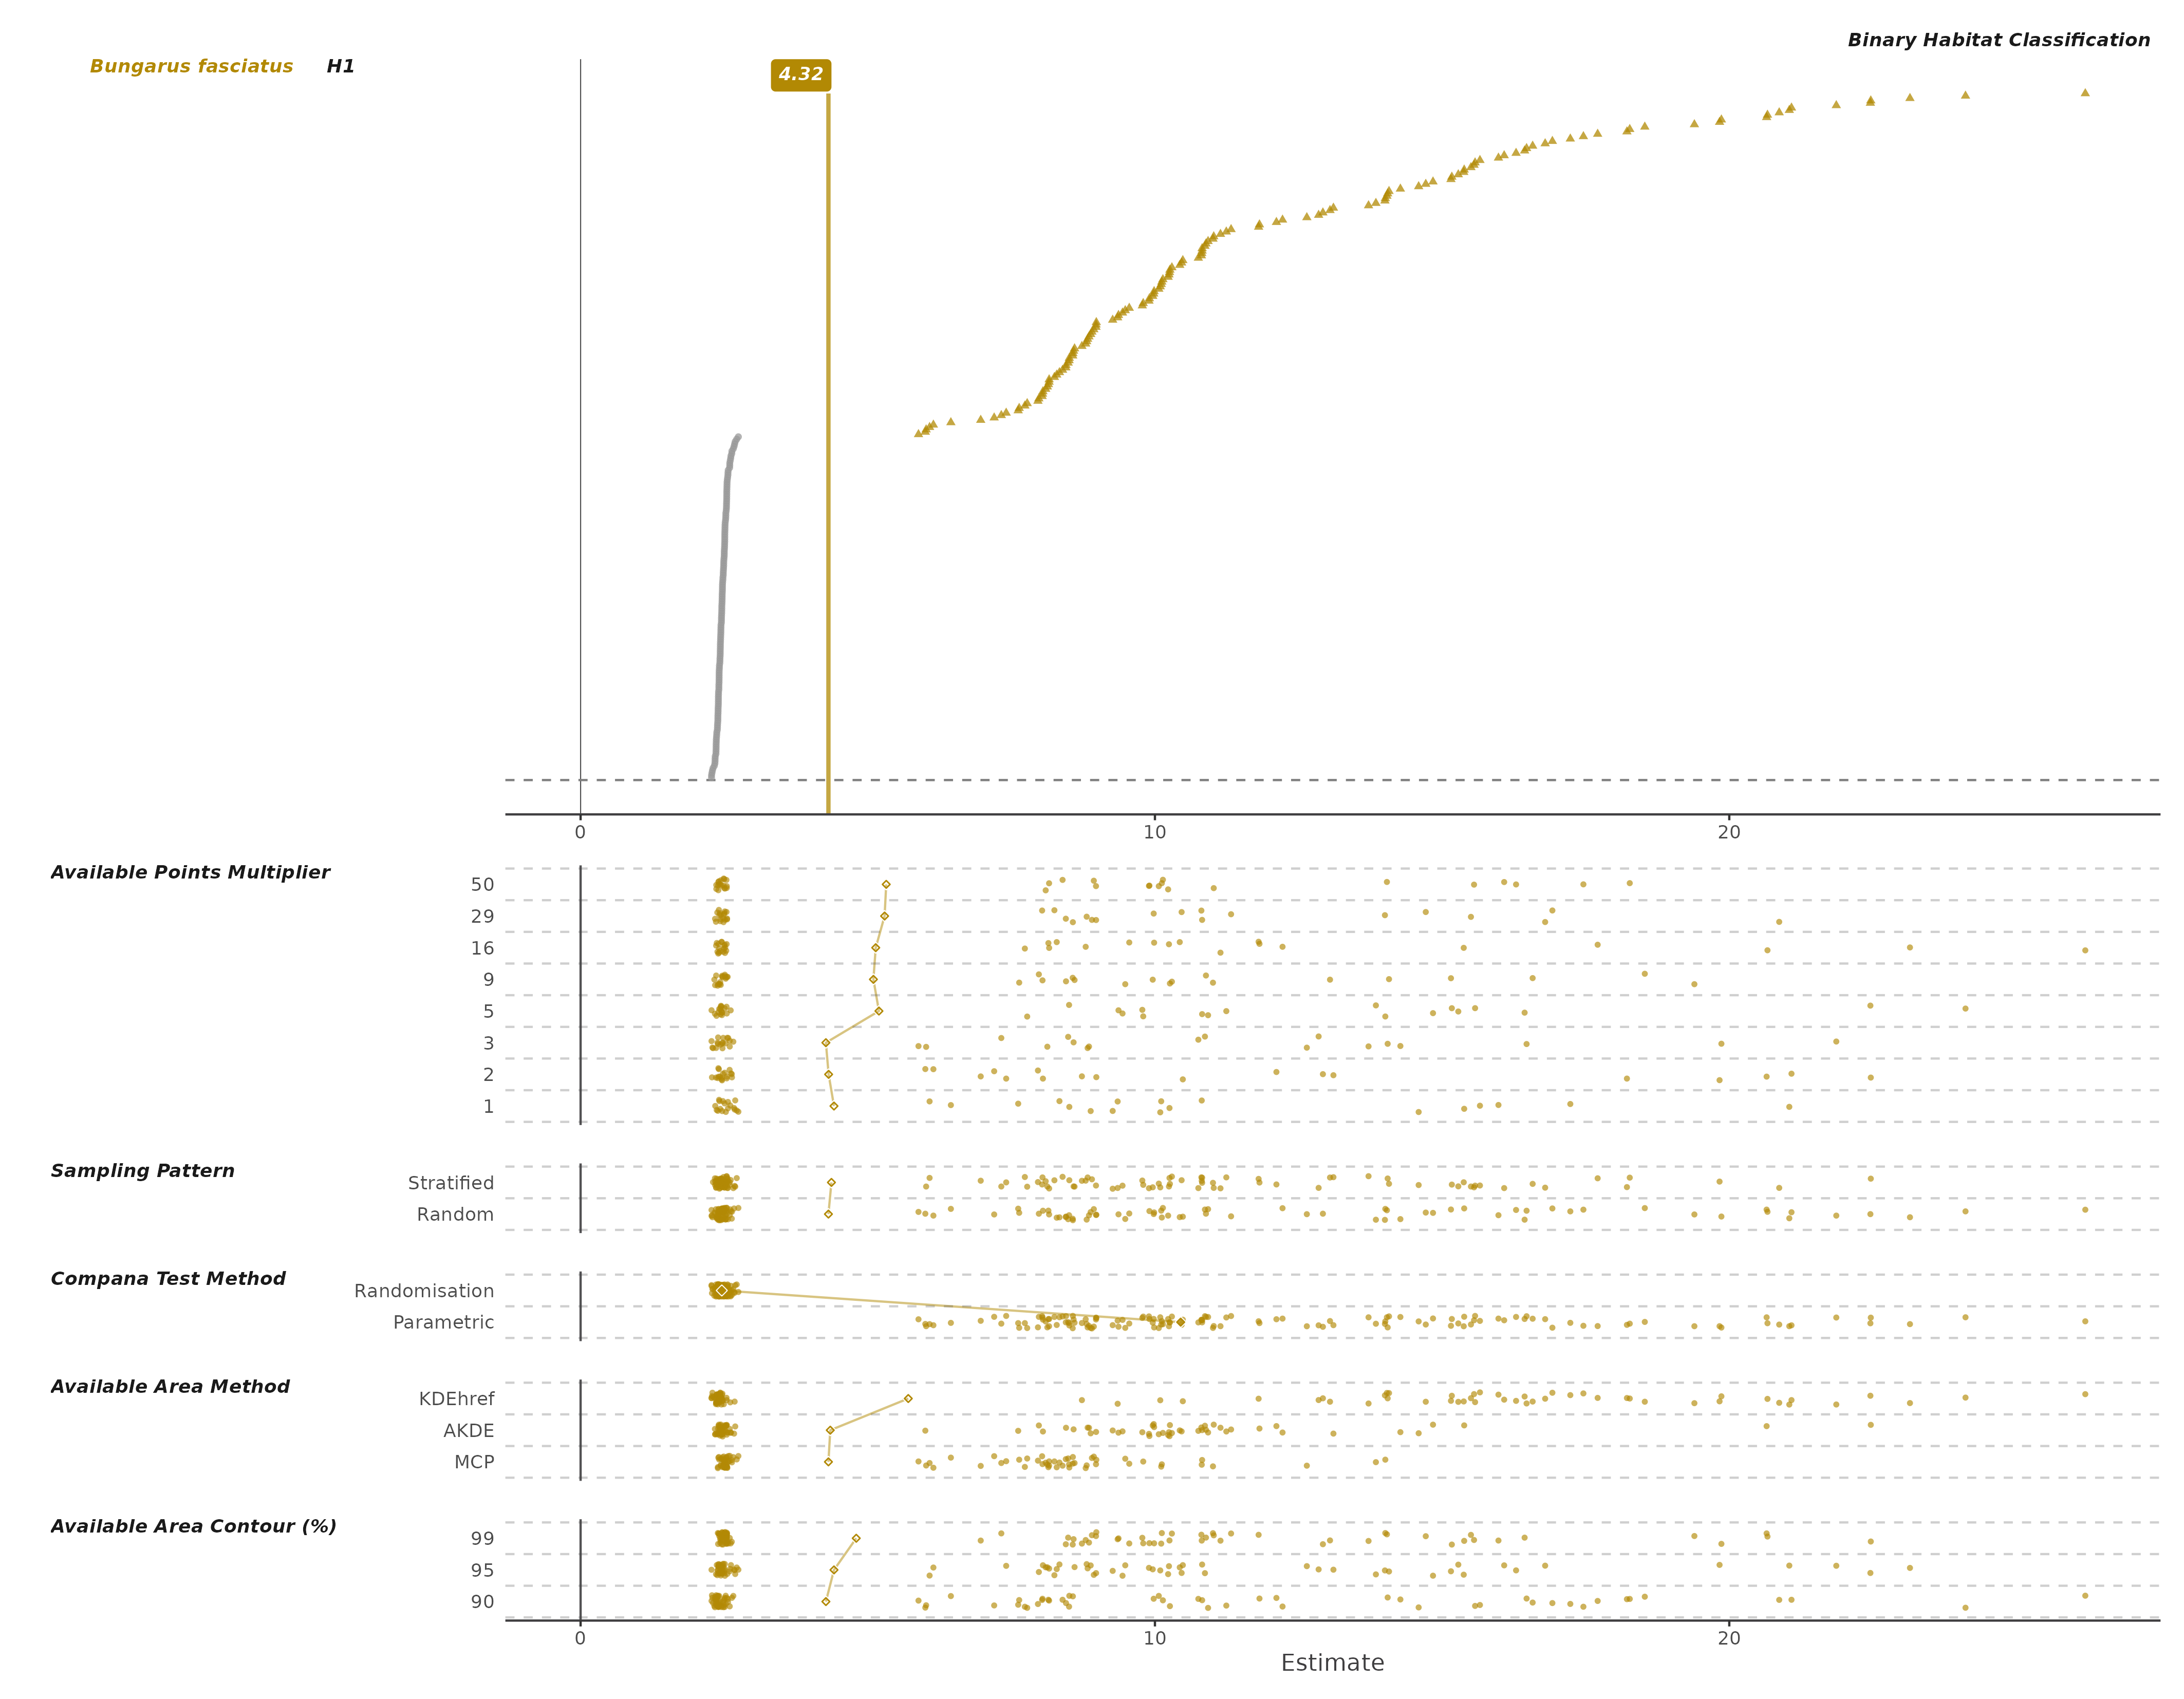
\includegraphics[width=1\linewidth]{../../figures/specCurve_Bungarus fasciatus_area} \caption{All estimates of habitat selection derived from the areas-based Compositional (Compana) analysis for Banded Kraits (Bungarus fasciatus). Top curves show all estimates with coloured points and corresponding confidence intervals indicating whether those estimates significantly support the hypothesis. Bottom right labels provide a count of estimates that significantly support the hypothesis out of the total estimates. Labelled vertical lines show the median point estimate. Lower plot show the estimates relative to each analysis choice. Median estimates are shown with hollow diamonds, and are connected with appropriated coloured lines.}\label{fig:specCurveAreaBUFA}
\end{figure}

\begin{figure}
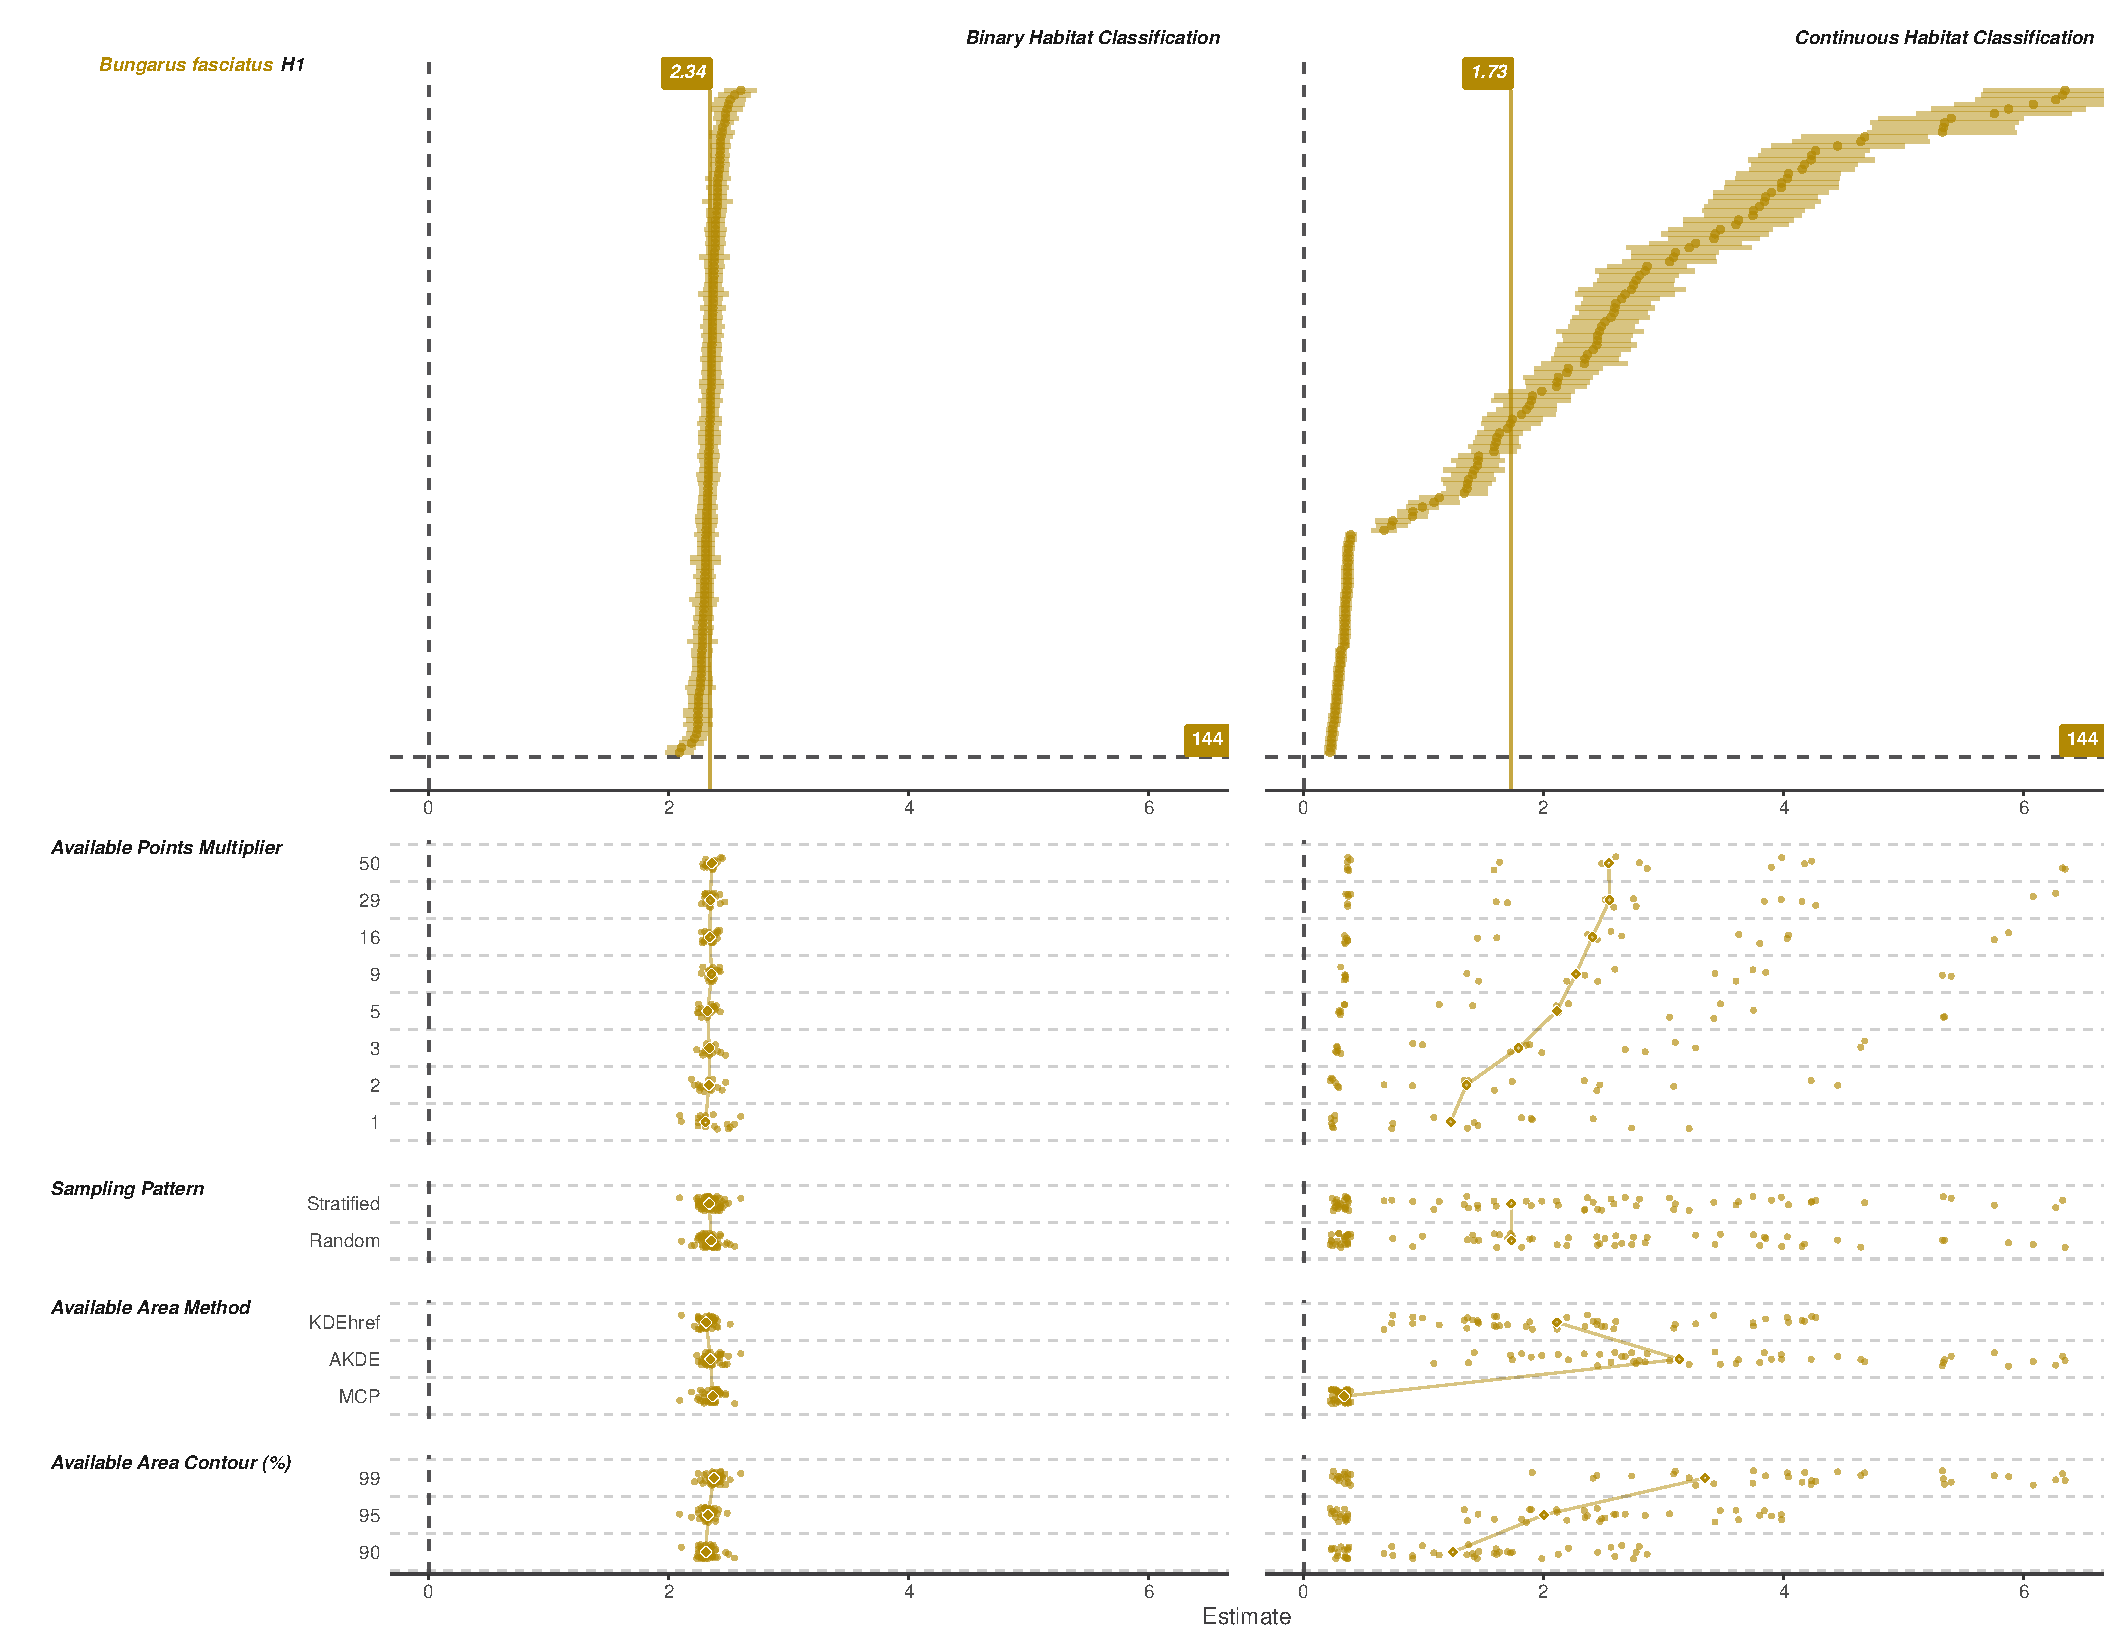
\includegraphics[width=1\linewidth]{../../figures/specCurve_Bungarus fasciatus_rsf} \caption{All estimates of habitat selection derived from the areas-based Resource Selection Function (RSF) analysis for Banded Kraits (Bungarus fasciatus). Top curves show all estimates with coloured points and corresponding confidence intervals indicating whether those estimates significantly support the hypothesis. Bottom right labels provide a count of estimates that significantly support the hypothesis out of the total estimates. Labelled vertical lines show the median point estimate. Lower plot show the estimates relative to each analysis choice. Median estimates are shown with hollow diamonds, and are connected with appropriated coloured lines. The plot is split left and right for the analysis using a binary classification (left), and continuous inverted distance (right).}\label{fig:specCurveRsfBUFA}
\end{figure}

\begin{figure}
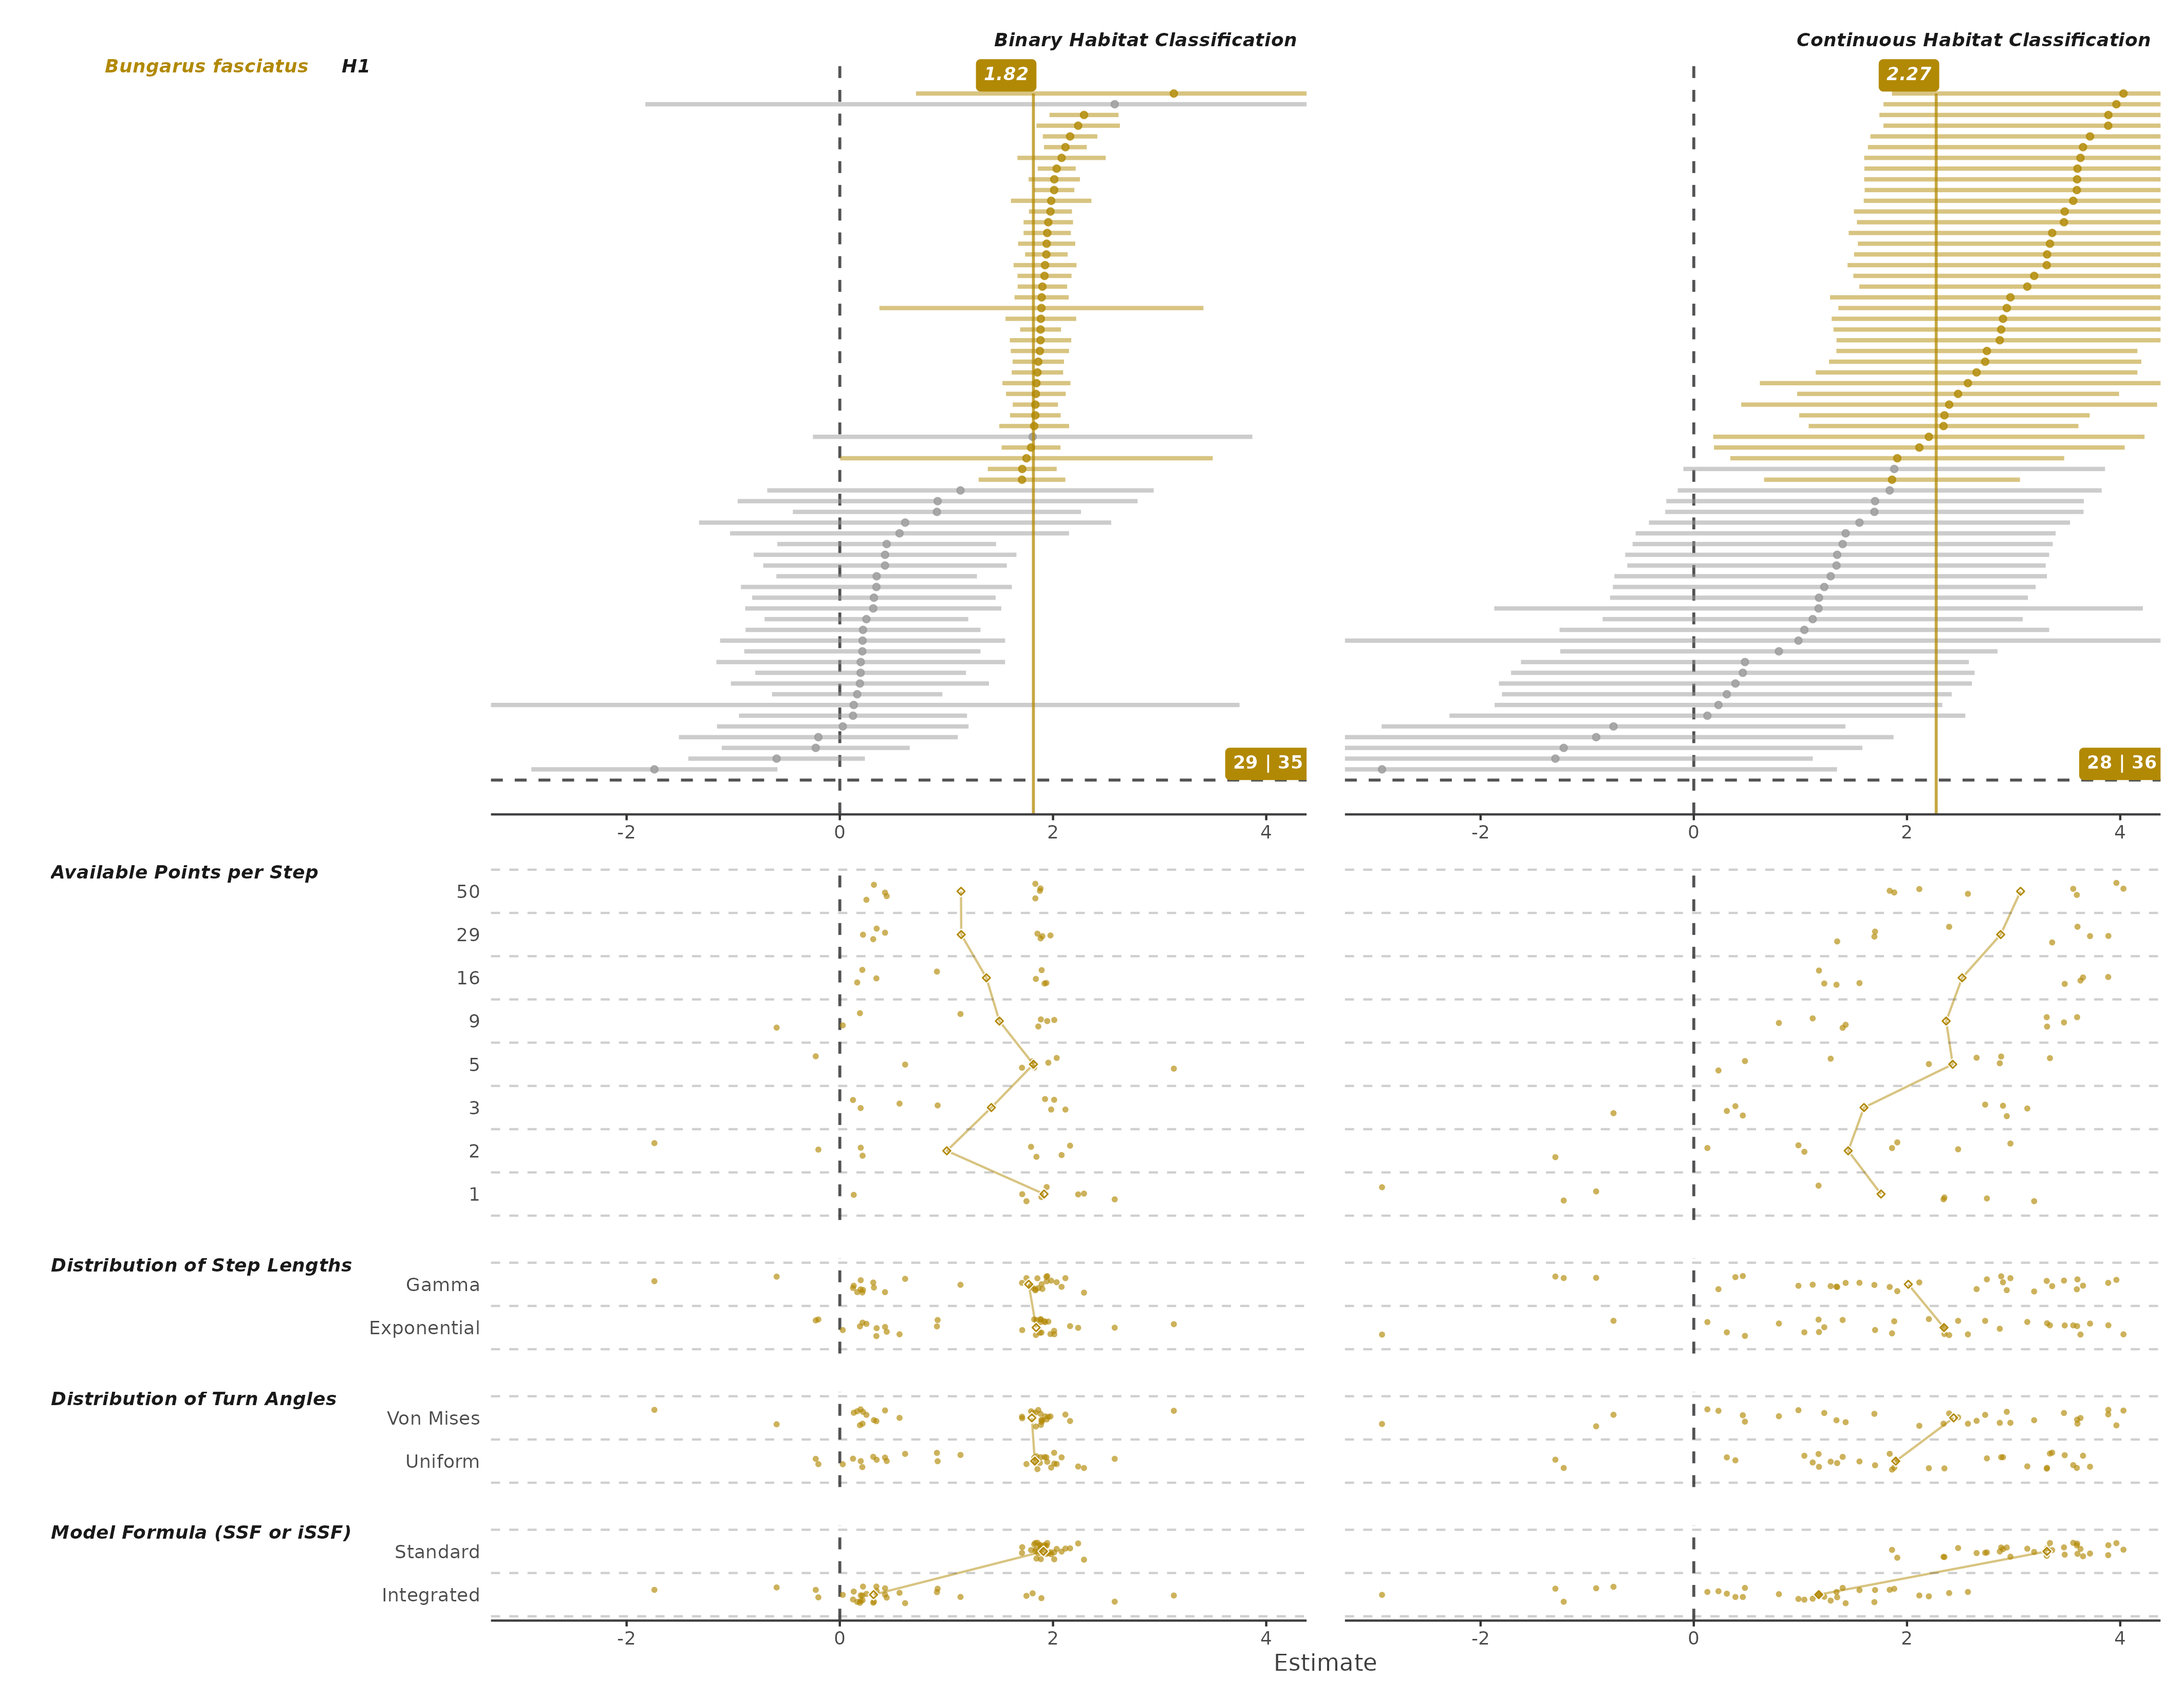
\includegraphics[width=1\linewidth]{../../figures/specCurve_Bungarus fasciatus_twoStep} \caption{All estimates of habitat selection derived from the step-based Two-Step analysis for Banded Kraits (Bungarus fasciatus). Top curves show all estimates with coloured points and corresponding confidence intervals indicating whether those estimates significantly support the hypothesis. Bottom right labels provide a count of estimates that significantly support the hypothesis out of the total estimates. Labelled vertical lines show the median point estimate. Lower plot show the estimates relative to each analysis choice. Median estimates are shown with hollow diamonds, and are connected with appropriated coloured lines. The plot is split left and right for the analysis using a binary classification (left), and continuous inverted distance (right).}\label{fig:specCurveTwoStepBUFA}
\end{figure}

\begin{figure}
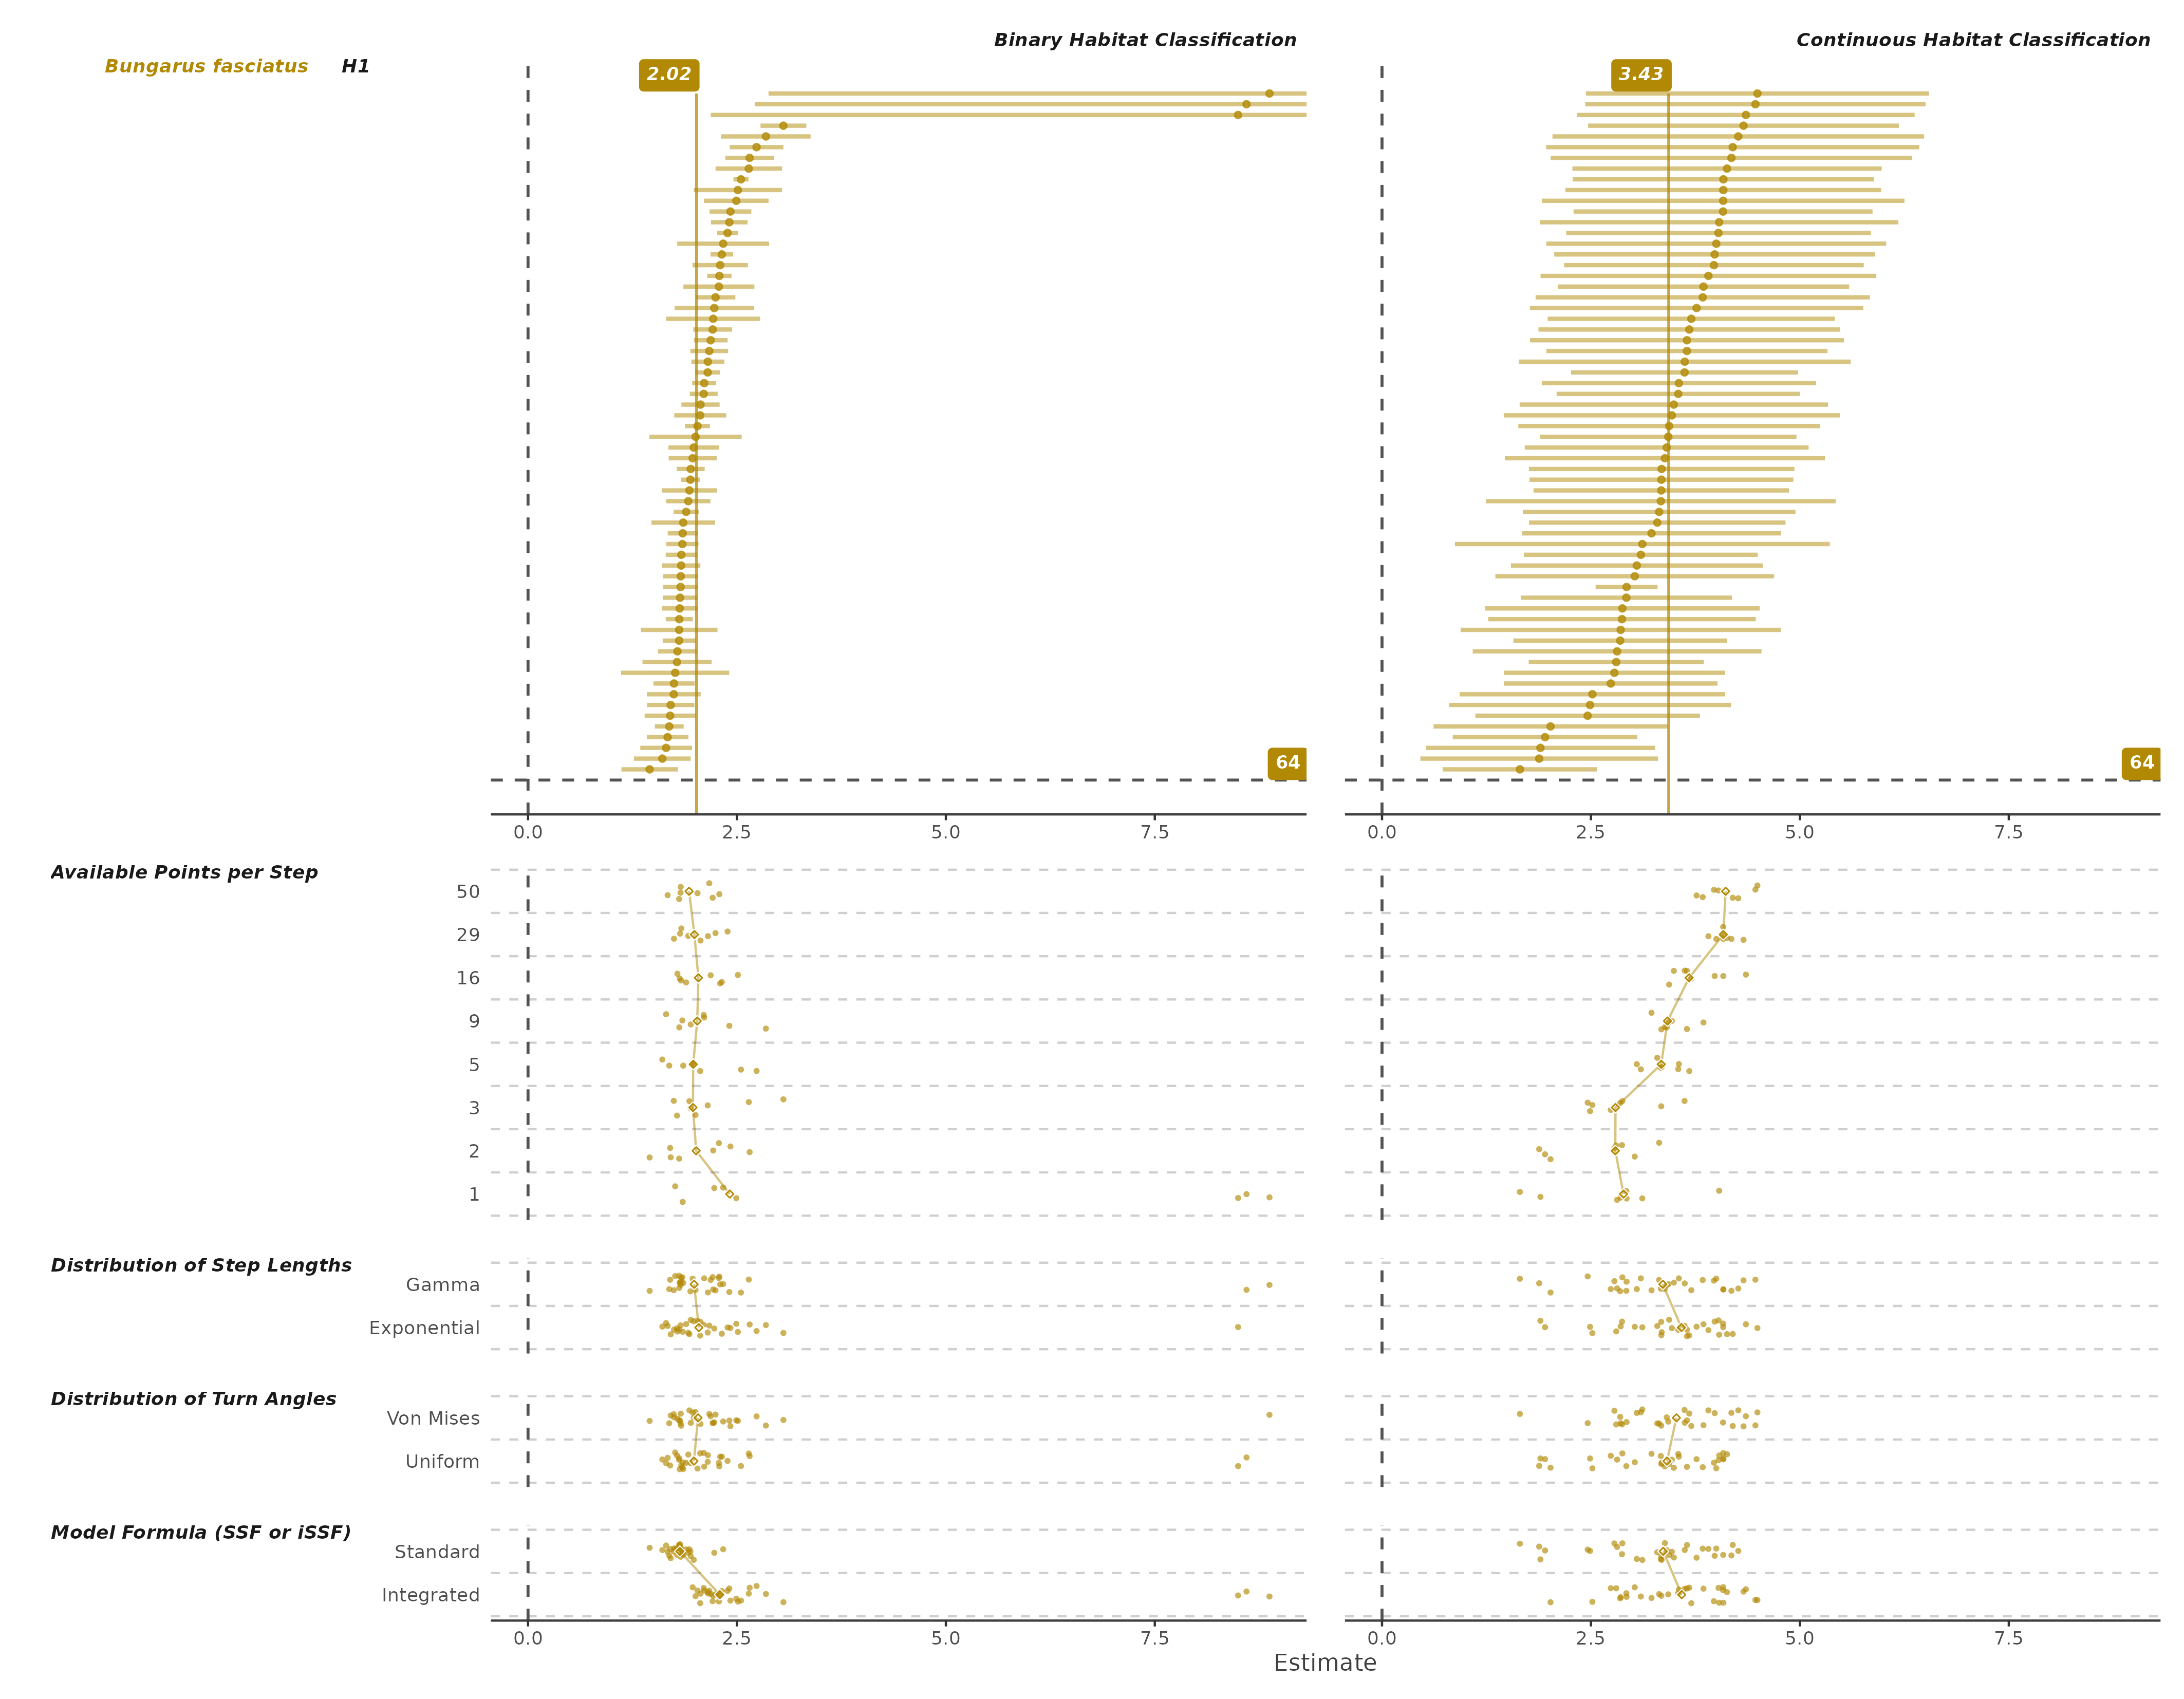
\includegraphics[width=1\linewidth]{../../figures/specCurve_Bungarus fasciatus_ssf} \caption{All estimates of habitat selection derived from the step-based Step Selection Function (SSF) analysis for Banded Kraits (Bungarus fasciatus). Top curves show all estimates with coloured points and corresponding confidence intervals indicating whether those estimates significantly support the hypothesis. Bottom right labels provide a count of estimates that significantly support the hypothesis out of the total estimates. Labelled vertical lines show the median point estimate. Lower plot show the estimates relative to each analysis choice. Median estimates are shown with hollow diamonds, and are connected with appropriated coloured lines. The plot is split left and right for the analysis using a binary classification (left), and continuous inverted distance (right).}\label{fig:specCurveSsfBUFA}
\end{figure}

\begin{figure}
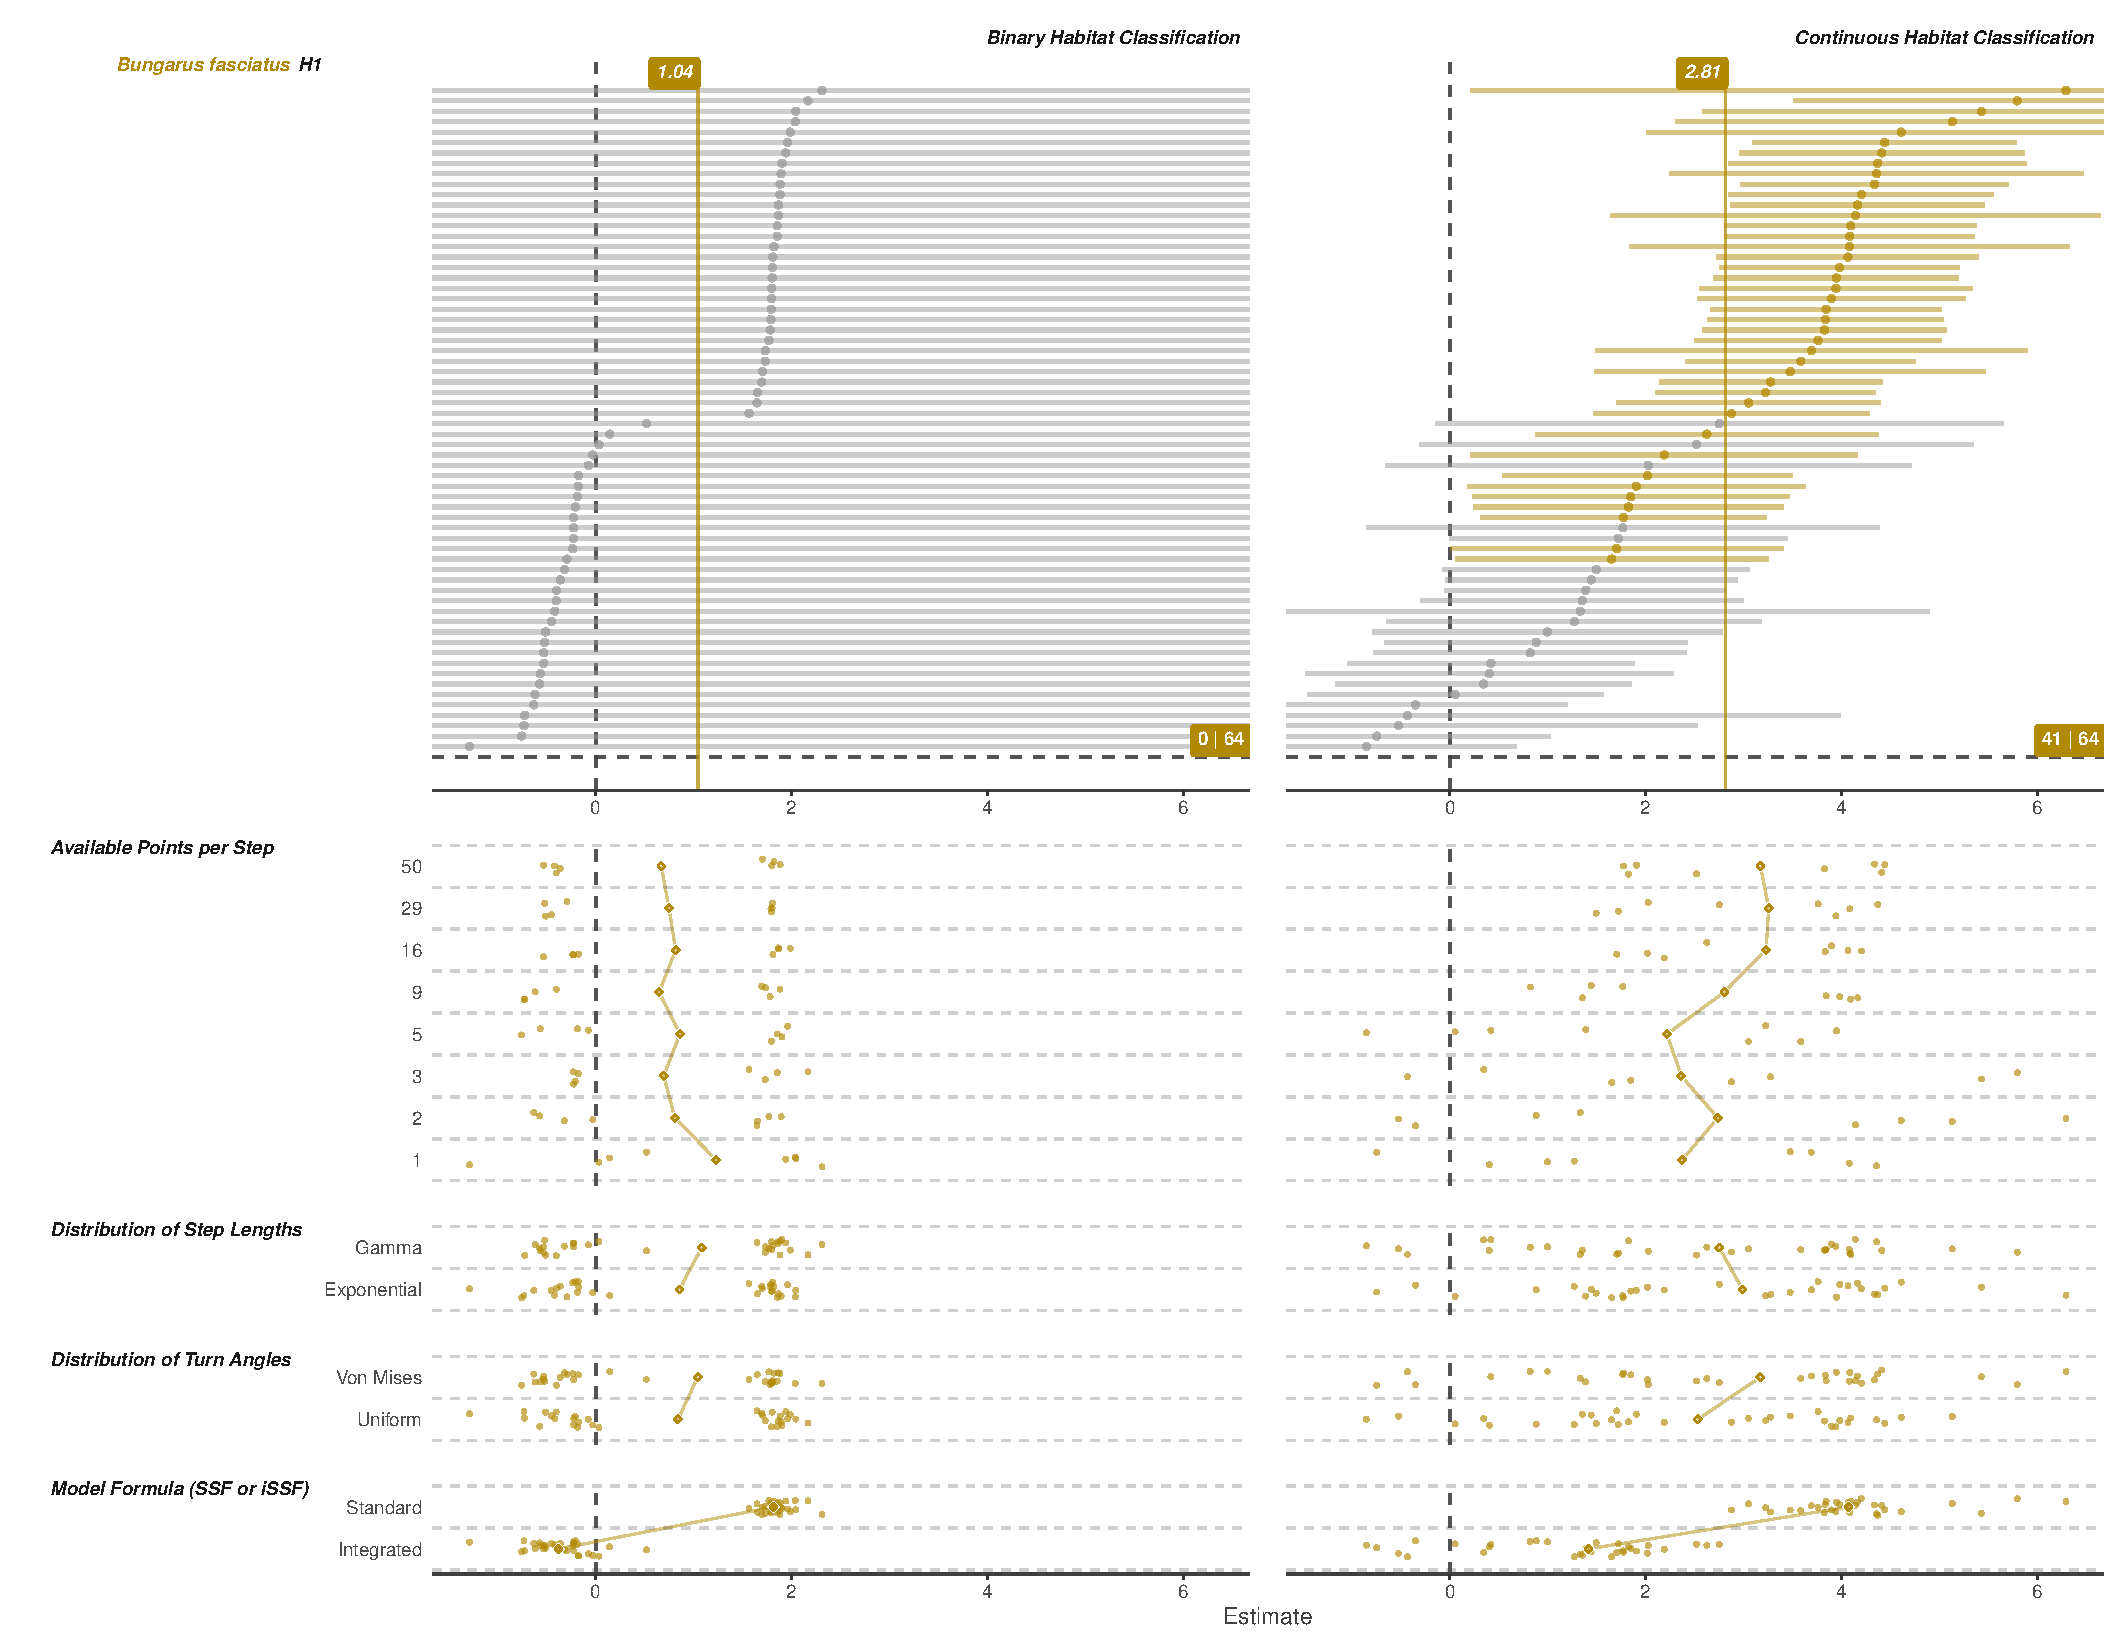
\includegraphics[width=1\linewidth]{../../figures/specCurve_Bungarus fasciatus_pois} \caption{All estimates of habitat selection derived from the step-based Poisson model (Poisson) analysis for Banded Kraits (Bungarus fasciatus). Top curves show all estimates with coloured points and corresponding confidence intervals indicating whether those estimates significantly support the hypothesis. Bottom right labels provide a count of estimates that significantly support the hypothesis out of the total estimates. Labelled vertical lines show the median point estimate. Lower plot show the estimates relative to each analysis choice. Median estimates are shown with hollow diamonds, and are connected with appropriated coloured lines. The plot is split left and right for the analysis using a binary classification (left), and continuous inverted distance (right).}\label{fig:specCurvePoisBUFA}
\end{figure}

\section*{References}\label{references}
\addcontentsline{toc}{section}{References}

\phantomsection\label{refs}
\begin{CSLReferences}{1}{0}
\bibitem[\citeproctext]{ref-alberts_self-correction_2015}
Alberts B, Cicerone RJ, Fienberg SE, Kamb A, McNutt M, Nerem RM, Schekman R, Shiffrin R, Stodden V, Suresh S, Zuber MT, Pope BK, Jamieson KH. 2015. Self-correction in science at work. \emph{Science} 348:1420--1422. DOI: \href{https://doi.org/10.1126/science.aab3847}{10.1126/science.aab3847}.

\bibitem[\citeproctext]{ref-rmarkdown2023}
Allaire J, Xie Y, Dervieux C, McPherson J, Luraschi J, Ushey K, Atkins A, Wickham H, Cheng J, Chang W, Iannone R. 2023. \emph{\href{https://github.com/rstudio/rmarkdown}{{rmarkdown}: Dynamic documents for r}}.

\bibitem[\citeproctext]{ref-alston_mitigating_2023}
Alston JM, Fleming CH, Kays R, Streicher JP, Downs CT, Ramesh T, Reineking B, Calabrese JM. 2023. Mitigating pseudoreplication and bias in resource selection functions with autocorrelation‐informed weighting. \emph{Methods in Ecology and Evolution} 14:643--654. DOI: \href{https://doi.org/10.1111/2041-210X.14025}{10.1111/2041-210X.14025}.

\bibitem[\citeproctext]{ref-altobelli_methods_2022}
Altobelli JT, Dickinson KJM, Godfrey SS, Bishop PJ. 2022. Methods in amphibian biotelemetry: {Two} decades in review. \emph{Austral Ecology} 47:1382--1395. DOI: \href{https://doi.org/10.1111/aec.13227}{10.1111/aec.13227}.

\bibitem[\citeproctext]{ref-barnes_snake_2024}
Barnes CH, Abdulaziz UZ, Kaenphet A, Kanlayanapaphon C. 2024. Snake diversity, occupancy, and detection on {Thailand}'s largest university campus. \emph{Ecology and Evolution} 14:e70317. DOI: \href{https://doi.org/10.1002/ece3.70317}{10.1002/ece3.70317}.

\bibitem[\citeproctext]{ref-Barnes2017}
Barnes CH, Strine CT, Suwanwaree P, Hill III JG. 2017. Movement and home range of green pit vipers ({Trimeresurus} spp.) in a rural landscape in north-east {Thailand}. \emph{Herpetological Bulletin} 142:19--28.

\bibitem[\citeproctext]{ref-barto_dissemination_2012}
Barto EK, Rillig MC. 2012. Dissemination biases in ecology: Effect sizes matter more than quality. \emph{Oikos} 121:228--235. DOI: \href{https://doi.org/10.1111/j.1600-0706.2011.19401.x}{10.1111/j.1600-0706.2011.19401.x}.

\bibitem[\citeproctext]{ref-bartoszek_natural_2018}
Bartoszek I, Andreadis PT, Prokop-Ervin C, Patel M, Reed RN. 2018. Natural {History} {Note}: {Python} bivittatus ({Burmese} {Python}). {Diet} and {Prey} {Size}. \emph{Herpetological Review} 49:139--140.

\bibitem[\citeproctext]{ref-lme4}
Bates D, Mächler M, Bolker B, Walker S. 2015. Fitting linear mixed-effects models using {lme4}. \emph{Journal of Statistical Software} 67:1--48. DOI: \href{https://doi.org/10.18637/jss.v067.i01}{10.18637/jss.v067.i01}.

\bibitem[\citeproctext]{ref-Bauder2016a}
Bauder JM, Breininger DR, Bolt MR, Legare ML, Jenkins CL, Rothermel BB, McGarigal K. 2016. Seasonal {Variation} in {Eastern} {Indigo} {Snake} ({Drymarchon} couperi) {Movement} {Patterns} and {Space} {Use} in {Peninsular} {Florida} at {Multiple} {Temporal} {Scales}. \emph{Herpetologica} 72:214--226. DOI: \href{https://doi.org/10.1655/Herpetologica-D-15-00039.1}{10.1655/Herpetologica-D-15-00039.1}.

\bibitem[\citeproctext]{ref-boback_use_2020}
Boback SM, Nafus MG, Yackel Adams AA, Reed RN. 2020. Use of visual surveys and radiotelemetry reveals sources of detection bias for a cryptic snake at low densities. \emph{Ecosphere} 11. DOI: \href{https://doi.org/10.1002/ecs2.3000}{10.1002/ecs2.3000}.

\bibitem[\citeproctext]{ref-brown_habitat_2001}
Brown PR, Singleton GR. 2001. Habitat use and movements of the rice-field rat, \emph{{Rattus} argentiventer} , in {West} {Java}, {Indonesia}. \emph{mamm} 65:151--166. DOI: \href{https://doi.org/10.1515/mamm.2001.65.2.151}{10.1515/mamm.2001.65.2.151}.

\bibitem[\citeproctext]{ref-brms}
Bürkner P-C. 2021. Bayesian item response modeling in {R} with {brms} and {Stan}. \emph{Journal of Statistical Software} 100:1--54. DOI: \href{https://doi.org/10.18637/jss.v100.i05}{10.18637/jss.v100.i05}.

\bibitem[\citeproctext]{ref-Calabrese2016}
Calabrese JM, Fleming CH, Gurarie E. 2016. Ctmm: An {R} {Package} for {Analyzing} {Animal} {Relocation} {Data} {As} a {Continuous}-{Time} {Stochastic} {Process}. \emph{Methods in Ecology and Evolution} 7:1124--1132. DOI: \href{https://doi.org/10.1111/2041-210X.12559}{10.1111/2041-210X.12559}.

\bibitem[\citeproctext]{ref-adehabitatHS}
Calenge C, Mathieu Basille contributions from. 2023. \emph{\href{https://CRAN.R-project.org/package=adehabitatHS}{{adehabitatHS}: Analysis of habitat selection by animals}}.

\bibitem[\citeproctext]{ref-adehabitatHR}
Calenge C, Scott Fortmann-Roe contributions from. 2023. \emph{\href{https://CRAN.R-project.org/package=adehabitatHR}{{adehabitatHR}: Home range estimation}}.

\bibitem[\citeproctext]{ref-ggnewscale}
Campitelli E. 2024. \emph{\href{https://CRAN.R-project.org/package=ggnewscale}{Ggnewscale: Multiple fill and colour scales in 'ggplot2'}}.

\bibitem[\citeproctext]{ref-qs}
Ching T. 2023. \emph{\href{https://CRAN.R-project.org/package=qs}{{qs}: Quick serialization of r objects}}.

\bibitem[\citeproctext]{ref-sfheaders}
Cooley D. 2023. \emph{\href{https://CRAN.R-project.org/package=sfheaders}{{sfheaders}: Converts between r objects and simple feature objects}}.

\bibitem[\citeproctext]{ref-TwoStepCLogit}
Craiu RV, Duchesne T, Fortin D, Baillargeon S. 2016. \emph{\href{https://CRAN.R-project.org/package=TwoStepCLogit}{TwoStepCLogit: Conditional logistic regression: A two-step estimation method}}.

\bibitem[\citeproctext]{ref-crane_supplementary_2020}
Crane MS, Silva IMS, Marshall BM, Strine CT. 2020. Supplementary files for {Crane} et al., "{Lots} of movement, little progress": {R} {Code}, data and figures. DOI: \href{https://doi.org/10.5281/ZENODO.4303887}{10.5281/ZENODO.4303887}.

\bibitem[\citeproctext]{ref-crane_lots_2021}
Crane M, Silva I, Marshall BM, Strine CT. 2021. Lots of movement, little progress: A review of reptile home range literature. \emph{PeerJ} 9:e11742. DOI: \href{https://doi.org/10.7717/peerj.11742}{10.7717/peerj.11742}.

\bibitem[\citeproctext]{ref-desbureaux_subjective_2021}
Desbureaux S. 2021. Subjective modeling choices and the robustness of impact evaluations in conservation science. \emph{Conservation Biology} 35:1615--1626. DOI: \href{https://doi.org/10.1111/cobi.13728}{10.1111/cobi.13728}.

\bibitem[\citeproctext]{ref-doherty_animal_2019}
Doherty TS, Fist CN, Driscoll DA. 2019. Animal movement varies with resource availability, landscape configuration and body size: A conceptual model and empirical example. \emph{Landscape Ecology} 34:603--614. DOI: \href{https://doi.org/10.1007/s10980-019-00795-x}{10.1007/s10980-019-00795-x}.

\bibitem[\citeproctext]{ref-dolia_house-warming_2023}
Dolia J, Das A, Kelkar N. 2023. House-warming: {Wild} king cobra nests have thermal regimes that positively affect hatching success and hatchling size. \emph{Journal of Thermal Biology} 112:103468. DOI: \href{https://doi.org/10.1016/j.jtherbio.2023.103468}{10.1016/j.jtherbio.2023.103468}.

\bibitem[\citeproctext]{ref-dorcas_severe_2012}
Dorcas ME, Willson JD, Reed RN, Snow RW, Rochford MR, Miller MA, Meshaka WE, Andreadis PT, Mazzotti FJ, Romagosa CM, Hart KM. 2012. Severe mammal declines coincide with proliferation of invasive {Burmese} pythons in {Everglades} {National} {Park}. \emph{Proceedings of the National Academy of Sciences} 109:2418--2422. DOI: \href{https://doi.org/10.1073/pnas.1115226109}{10.1073/pnas.1115226109}.

\bibitem[\citeproctext]{ref-Durso2015}
Durso AM, Seigel RA. 2015. A {Snake} in the {Hand} is {Worth} 10,000 in the {Bush}. \emph{Journal of Herpetology} 49:503--506. DOI: \href{https://doi.org/10.1670/15-49-04.1}{10.1670/15-49-04.1}.

\bibitem[\citeproctext]{ref-Duvall1997}
Duvall D, Schuett GW. 1997. Straight-line movement and competitive mate searching in prairie rattlesnakes, {Crotalus} viridis viridis. \emph{Animal Behaviour} 54:329--334. DOI: \href{https://doi.org/10.1006/anbe.1996.0418}{10.1006/anbe.1996.0418}.

\bibitem[\citeproctext]{ref-Fleming2017}
Fleming CH, Calabrese JM. 2017. A new kernel density estimator for accurate home-range and species-range area estimation. \emph{Methods in Ecology and Evolution} 8:571--579. DOI: \href{https://doi.org/10.1111/2041-210X.12673}{10.1111/2041-210X.12673}.

\bibitem[\citeproctext]{ref-ctmm}
Fleming CH, Calabrese JM. 2023. \emph{{ctmm}: Continuous-time movement modeling}.

\bibitem[\citeproctext]{ref-Fleming2015}
Fleming CH, Fagan WF, Mueller T, Olson KA, Leimgruber P, Calabrese JM. 2015. Rigorous home range estimation with movement data: {A} new autocorrelated kernel density estimator. \emph{Ecology} 96:1182--1188.

\bibitem[\citeproctext]{ref-forester_accounting_2009}
Forester JD, Im HK, Rathouz PJ. 2009. Accounting for animal movement in estimation of resource selection functions: Sampling and data analysis. \emph{Ecology} 90:3554--3565. DOI: \href{https://doi.org/10.1890/08-0874.1}{10.1890/08-0874.1}.

\bibitem[\citeproctext]{ref-grateful}
Francisco Rodríguez-Sánchez, Connor P. Jackson, Shaurita D. Hutchins. 2023. \emph{\href{https://github.com/Pakillo/grateful}{{grateful}: Facilitate citation of r packages}}.

\bibitem[\citeproctext]{ref-fujioka_bird_2010}
Fujioka M, Don Lee S, Kurechi M. 2010. Bird use of {Rice} {Fields} in {Korea} and {Japan}. \emph{Waterbirds} 33:8. DOI: \href{https://doi.org/10.1675/063.033.s102}{10.1675/063.033.s102}.

\bibitem[\citeproctext]{ref-bayesplot}
Gabry J, Mahr T. 2024. \href{https://mc-stan.org/bayesplot/}{Bayesplot: Plotting for bayesian models}.

\bibitem[\citeproctext]{ref-goldstein_integrating_2021}
Goldstein E, Erinjery JJ, Martin G, Kasturiratne A, Ediriweera DS, Silva HJ de, Diggle P, Lalloo DG, Murray KA, Iwamura T. 2021. Integrating human behavior and snake ecology with agent-based models to predict snakebite in high risk landscapes. \emph{PLOS Neglected Tropical Diseases} 15:e0009047. DOI: \href{https://doi.org/10.1371/journal.pntd.0009047}{10.1371/journal.pntd.0009047}.

\bibitem[\citeproctext]{ref-gould_same_2023}
Gould E, Fraser H, Parker T, Nakagawa S, Griffith S, Vesk P, Fidler F, Abbey-Lee R, Abbott J, Aguirre L, Alcaraz C, Altschul D, Arekar K, Atkins J, Atkinson J, Barrett M, Bell K, Bello S, Berauer B, Bertram M, Billman P, Blake C, Blake S, Bliard L, Bonisoli-Alquati A, Bonnet T, Bordes C, Bose A, Botterill-James T, Boyd M, Boyle S, Bradfer-Lawrence T, Brand J, Brengdahl M, Bulla M, Bussière L, Camerlenghi E, Campbell S, Campos L, Caravaggi A, Cardoso P, Carroll C, Catanach T, Chen X, Chik HYJ, Choy E, Christie A, Chuang A, Chunco A, Clark B, Cox M, Cressman K, Crouch C, D'Amelio P, De Sousa A, Döbert T, Dobler R, Dobson A, Doherty T, Drobniak S, Duffy A, Dunn R, Dunning J, Eberhart-Hertel L, Elmore J, Elsherif M, English H, Ensminger D, Ernst U, Ferguson S, Ferreira-Arruda T, Fieberg J, Finch E, Fiorenza E, Fisher D, Forstmeier W, Fourcade Y, Francesca Santostefano F, Frank G, Freund C, Gandy S, Gannon D, García-Cervigón A, Géron C, Gilles M, Girndt A, Gliksman D, Goldspiel H, Gomes D, Goslee S, Gosnell J, Gratton P, Grebe N, Greenler S, Griffith D, Griffith F, Grossman J, Güncan A, Haesen S, Hagan J, Harrison N, Hasnain S, Havird J, Heaton A, Hsu B-Y, Iranzo E, Iverson E, Jimoh S, Johnson D, Johnsson M, Jorna J, Jucker T, Jung M, Kačergytė I, Ke A, Kelly C, Keogan K, Keppeler F, Killion A, Kim D, Kochan D, Korsten P, Kothari S, Kuppler J, Kusch J, Lagisz M, Larkin D, Larson C, Lauck K, Lauterbur M, Law A, Léandri-Breton D-J, Lievens E, Lima D, Lindsay S, Macphie K, Mair M, Malm L, Mammola S, Manhart M, Mäntylä E, Marchand P, Marshall B, Martin D, Martin J, Martin C, Martinig A, McCallum E, McNew S, Meiners S, Michelangeli M, Moiron M, Moreira B, Mortensen J, Mos B, Muraina T, Nelli L, Nilsonne G, Nolazco S, Nooten S, Novotny J, Olin A, Organ C, Ostevik K, Palacio F, Paquet M, Pascall D, Pasquarella V, Payo-Payo A, Pedersen K, Perez G, Perry K, Pottier P, Proulx M, Proulx R, Pruett J, Ramananjato V, Randimbiarison F, Razafindratsima O, Rennison D, Riva F, Riyahi S, Roast M, Rocha F, Roche D, Román-Palacios C, Rosenberg M, Ross J, Rowland F, Rugemalila D, Russell A, Ruuskanen S, Saccone P, Sadeh A, Salazar S, Sales K, Salmón P, Sanchez-Tojar A, Santos L, Schilling H, Schmidt M, Schmoll T, Schneider A, Schrock A, Schroeder J, Schtickzelle N, Schultz N, Scott D, Shapiro J, Sharma N, Shearer C, Sitvarin M, Skupien F, Slinn H, Smith J, Smith G, Sollmann R, Stack Whitney K, Still S, Stuber E, Sutton G, Swallow B, Taff C, Takola E, Tanentzap A, Thawley C, Tortorelli C, Trlica A, Turnell B, Urban L, Van De Vondel S, Van Oordt F, Vanderwel M, Vanderwel K, Vanderwolf K, Verrelli B, Vieira M, Vollering J, Walker X, Walter J, Waryszak P, Weaver R, Weller D, Whelan S, White R, Wolfson D, Wood A, Yanco S, Yen J, Youngflesh C, Zilio G, Zimmer C, Zitomer R, Villamil N, Tompkins E. 2023. Same data, different analysts: Variation in effect sizes due to analytical decisions in ecology and evolutionary biology. \emph{EcoEvoRxiv}. DOI: \href{https://doi.org/10.32942/X2GG62}{10.32942/X2GG62}.

\bibitem[\citeproctext]{ref-groffen_preference_2018}
Groffen J, Borzée A, Jang Y. 2018. Preference for natural borders in rice paddies by two treefrog species. \emph{Animal Cells and Systems} 22:205--211. DOI: \href{https://doi.org/10.1080/19768354.2018.1475301}{10.1080/19768354.2018.1475301}.

\bibitem[\citeproctext]{ref-tidyterra}
Hernangómez D. 2023. Using the {tidyverse} with {terra} objects: The {tidyterra} package. \emph{Journal of Open Source Software} 8:5751. DOI: \href{https://doi.org/10.21105/joss.05751}{10.21105/joss.05751}.

\bibitem[\citeproctext]{ref-raster}
Hijmans RJ. 2023a. \emph{\href{https://CRAN.R-project.org/package=raster}{{raster}: Geographic data analysis and modeling}}.

\bibitem[\citeproctext]{ref-terra}
Hijmans RJ. 2023b. \emph{\href{https://CRAN.R-project.org/package=terra}{{terra}: Spatial data analysis}}.

\bibitem[\citeproctext]{ref-hodges_deadly_2021}
Hodges CW, Barnes CH, Patungtaro P, Strine CT. 2021a. Deadly dormmate: {A} case study on {Bungarus} {candidus} living among a student dormitory with implications for human safety. \emph{Ecological Solutions and Evidence} 2. DOI: \href{https://doi.org/10.1002/2688-8319.12047}{10.1002/2688-8319.12047}.

\bibitem[\citeproctext]{ref-hodges_diurnal_2020}
Hodges CW, D'souza A, Jintapirom S. 2020. Diurnal observation of a {Malayan} {Krait} {Bungarus} candidus ({Reptilia}: {Elapidae}) feeding inside a building in {Thailand}. \emph{Journal of Threatened Taxa} 12:15947--15950. DOI: \href{https://doi.org/10.11609/jott.5746.12.8.15947-15950}{10.11609/jott.5746.12.8.15947-15950}.

\bibitem[\citeproctext]{ref-hodges_malayan_2021}
Hodges CW, Marshall BM, Hill III JG, Strine CT. 2021b. Malayan kraits ({Bungarus} candidus) show affinity to anthropogenic structures in a human dominated landscape. DOI: \href{https://doi.org/10.5281/ZENODO.5495839}{10.5281/ZENODO.5495839}.

\bibitem[\citeproctext]{ref-hodges_malayan_2022}
Hodges CW, Marshall BM, Hill JG, Strine CT. 2022. Malayan kraits ({Bungarus} candidus) show affinity to anthropogenic structures in a human dominated landscape. \emph{Scientific Reports} 12:7139. DOI: \href{https://doi.org/10.1038/s41598-022-11255-z}{10.1038/s41598-022-11255-z}.

\bibitem[\citeproctext]{ref-huntingtonklein_influence_2021}
Huntington‐Klein N, Arenas A, Beam E, Bertoni M, Bloem JR, Burli P, Chen N, Grieco P, Ekpe G, Pugatch T, Saavedra M, Stopnitzky Y. 2021. The influence of hidden researcher decisions in applied microeconomics. \emph{Economic Inquiry} 59:944--960. DOI: \href{https://doi.org/10.1111/ecin.12992}{10.1111/ecin.12992}.

\bibitem[\citeproctext]{ref-jennions_relationships_2002}
Jennions MD, Møller AP. 2002. Relationships fade with time: A meta-analysis of temporal trends in publication in ecology and evolution. \emph{Proceedings of the Royal Society of London. Series B: Biological Sciences} 269:43--48. DOI: \href{https://doi.org/10.1098/rspb.2001.1832}{10.1098/rspb.2001.1832}.

\bibitem[\citeproctext]{ref-Jones_supposed_2020}
Jones MD, Crane MS, Silva IMS, Artchawakom T, Waengsothorn S, Suwanwaree P, Strine CT, Goode M. 2020. Supposed snake specialist consumes monitor lizards: Diet and trophic implications of king cobra feeding ecology. \emph{Ecology}. DOI: \href{https://doi.org/10.1002/ecy.3085}{10.1002/ecy.3085}.

\bibitem[\citeproctext]{ref-jones_how_2022}
Jones MD, Marshall BM, Smith SN, Crane M, Silva I, Artchawakom T, Suwanwaree P, Waengsothorn S, Wüster W, Goode M, Strine CT. 2022. How do {King} {Cobras} move across a major highway? {Unintentional} wildlife crossing structures may facilitate movement. \emph{Ecology and Evolution} 12. DOI: \href{https://doi.org/10.1002/ece3.8691}{10.1002/ece3.8691}.

\bibitem[\citeproctext]{ref-joo_recent_2022}
Joo R, Picardi S, Boone ME, Clay TA, Patrick SC, Romero-Romero VS, Basille M. 2022. Recent trends in movement ecology of animals and human mobility. \emph{Movement Ecology} 10:26. DOI: \href{https://doi.org/10.1186/s40462-022-00322-9}{10.1186/s40462-022-00322-9}.

\bibitem[\citeproctext]{ref-ggdist}
Kay M. 2023a. \emph{{ggdist}: Visualizations of distributions and uncertainty}. DOI: \href{https://doi.org/10.5281/zenodo.3879620}{10.5281/zenodo.3879620}.

\bibitem[\citeproctext]{ref-tidybayes}
Kay M. 2023b. \emph{{tidybayes}: Tidy data and geoms for {Bayesian} models}. DOI: \href{https://doi.org/10.5281/zenodo.1308151}{10.5281/zenodo.1308151}.

\bibitem[\citeproctext]{ref-Kay2016}
Kay GM, Mortelliti A, Tulloch A, Barton P, Florance D, Cunningham SA, Lindenmayer DB. 2016. Effects of past and present livestock grazing on herpetofauna in a landscape-scale experiment. \emph{Conservation Biology} 31:446--458. DOI: \href{https://doi.org/10.1111/cobi.12779}{10.1111/cobi.12779}.

\bibitem[\citeproctext]{ref-kays_movebank_2022}
Kays R, Davidson SC, Berger M, Bohrer G, Fiedler W, Flack A, Hirt J, Hahn C, Gauggel D, Russell B, Kölzsch A, Lohr A, Partecke J, Quetting M, Safi K, Scharf A, Schneider G, Lang I, Schaeuffelhut F, Landwehr M, Storhas M, Schalkwyk L, Vinciguerra C, Weinzierl R, Wikelski M. 2022. The {Movebank} system for studying global animal movement and demography. \emph{Methods in Ecology and Evolution} 13:419--431. DOI: \href{https://doi.org/10.1111/2041-210X.13767}{10.1111/2041-210X.13767}.

\bibitem[\citeproctext]{ref-kelly_rate_2019}
Kelly CD. 2019. Rate and success of study replication in ecology and evolution. \emph{PeerJ} 7:e7654. DOI: \href{https://doi.org/10.7717/peerj.7654}{10.7717/peerj.7654}.

\bibitem[\citeproctext]{ref-knierim_spatial_2019}
Knierim T. 2019. Spatial ecology study reveals nest attendance and habitat preference of banded kraits ({Bungarus} fasciatus). \emph{Herpetological Bulletin}:6--13. DOI: \href{https://doi.org/10.33256/hb150.613}{10.33256/hb150.613}.

\bibitem[\citeproctext]{ref-Knierim2017a}
Knierim T, Barnes CH, Hodges C. 2017. BUNGARUS FASCIATUS banded krait. DIET SCAVENGING. \emph{Herpetological Review} 48:215--218.

\bibitem[\citeproctext]{ref-koirala_distribution_2021}
Koirala BK, Dawa Tshering. 2021. Distribution, habitat use, and nesting behavior of the {King} {Cobra} ({Ophiophagus} hannah) in the {Trashigang} {Forest} {Division}, {Eastern} {Bhutan}. \emph{Reptiles \& Amphibians} 28:397--403. DOI: \href{https://doi.org/10.17161/randa.v28i3.15786}{10.17161/randa.v28i3.15786}.

\bibitem[\citeproctext]{ref-move}
Kranstauber B, Smolla M, Scharf AK. 2023. \emph{\href{https://CRAN.R-project.org/package=move}{{move}: Visualizing and analyzing animal track data}}.

\bibitem[\citeproctext]{ref-kuch_notes_2001}
Kuch U. 2001. {NOTES} {ON} {THE} {DIET} {OF} {THE} {MALAYAN} {KRAIT}, {BUNGARUS} {CANDIDUS} ({LINNAEUS}, 1758). \emph{Herpetological Bulletin} 75.

\bibitem[\citeproctext]{ref-land_development_department_thailand_land-use_2017}
Land Development Department T. 2017. Land-use data of {Thailand}.

\bibitem[\citeproctext]{ref-tarchetypes}
Landau WM. 2021b. \emph{Tarchetypes: Archetypes for targets}.

\bibitem[\citeproctext]{ref-targets}
Landau WM. 2021a. \href{https://doi.org/10.21105/joss.02959}{The targets r package: A dynamic make-like function-oriented pipeline toolkit for reproducibility and high-performance computing}. \emph{Journal of Open Source Software} 6:2959.

\bibitem[\citeproctext]{ref-INLA}
Lindgren F, Rue H. 2015. \href{http://www.jstatsoft.org/v63/i19/}{Bayesian spatial modelling with {R}-{INLA}}. \emph{Journal of Statistical Software} 63:1--25.

\bibitem[\citeproctext]{ref-looareesuwan_factors_1988}
Looareesuwan S, Viravan C, Warrell DA. 1988. Factors contributing to fatal snake bite in the rural tropics: Analysis of 46 cases in {Thailand}. \emph{Transactions of The Royal Society of Tropical Medicine and Hygiene} 82:930--934. DOI: \href{https://doi.org/10.1016/0035-9203(88)90046-6}{10.1016/0035-9203(88)90046-6}.

\bibitem[\citeproctext]{ref-performance}
Lüdecke D, Ben-Shachar MS, Patil I, Waggoner P, Makowski D. 2021. {performance}: An {R} package for assessment, comparison and testing of statistical models. \emph{Journal of Open Source Software} 6:3139. DOI: \href{https://doi.org/10.21105/joss.03139}{10.21105/joss.03139}.

\bibitem[\citeproctext]{ref-marshall_no_2020}
Marshall BM, Crane M, Silva I, Strine CT, Jones MD, Hodges CW, Suwanwaree P, Artchawakom T, Waengsothorn S, Goode M. 2020a. No room to roam: {King} {Cobras} reduce movement in agriculture. \emph{Movement Ecology} 8:33. DOI: \href{https://doi.org/10.1186/s40462-020-00219-5}{10.1186/s40462-020-00219-5}.

\bibitem[\citeproctext]{ref-marshall_data_2020}
Marshall BM, Crane M, Silva I, Strine CT, Jones MD, Hodges CW, Suwanwaree P, Taksin Artchawakom, Surachit Waengsothorn, Goode M. 2020b. Data set and code supporting {Marshall} et al. 2020. {No} room to roam: {King} {Cobras} reduce movement in agriculture. DOI: \href{https://doi.org/10.5281/ZENODO.3666028}{10.5281/ZENODO.3666028}.

\bibitem[\citeproctext]{ref-marshall_habitat_2024}
Marshall BM, Duthie AB. 2024. A {Habitat} {Selection} {Multiverse} {Reveals} {Largely} {Consistent} {Results} {Despite} a {Multitude} of {Analysis} {Options}. \emph{bioRxiv}. DOI: \href{https://doi.org/10.1101/2024.06.19.599733}{10.1101/2024.06.19.599733}.

\bibitem[\citeproctext]{ref-Marshall2018}
Marshall BM, Strine CT, Jones MD, Artchawakom T, Silva I, Suwanwaree P, Goode M. 2019. Space fit for a king: Spatial ecology of king cobras ({Ophiophagus} hannah) in {Sakaerat} {Biosphere} {Reserve}, {Northeastern} {Thailand}. \emph{Amphibia-Reptilia} 40:163--178. DOI: \href{https://doi.org/10.1163/15685381-18000008}{10.1163/15685381-18000008}.

\bibitem[\citeproctext]{ref-Marshall2018b}
Marshall BM, Strine CT, Jones MD, Theodorou A, Amber E, Waengsothorn S, Suwanwaree P, Goode M. 2018. Hits {Close} to {Home}: {Repeated} {Persecution} of {King} {Cobras} ({Ophiophagus} hannah) in {Northeastern} {Thailand}. \emph{Tropical Conservation Science} 11:194008291881840. DOI: \href{https://doi.org/10.1177/1940082918818401}{10.1177/1940082918818401}.

\bibitem[\citeproctext]{ref-INLA2}
Martins TG, Simpson D, Lindgren F, Rue H. 2013. Bayesian computing with {INLA}: {N}ew features. \emph{Computational Statistics and Data Analysis} 67:68--83.

\bibitem[\citeproctext]{ref-michelot_langevin_2019}
Michelot T, Gloaguen P, Blackwell PG, Étienne M. 2019. The {Langevin} diffusion as a continuous‐time model of animal movement and habitat selection. \emph{Methods in Ecology and Evolution} 10:1894--1907. DOI: \href{https://doi.org/10.1111/2041-210X.13275}{10.1111/2041-210X.13275}.

\bibitem[\citeproctext]{ref-Miranda2016}
Miranda EBP, Ribeiro- RP, Strüssmann C. 2016. The ecology of human-anaconda conflict: A study using internet videos. \emph{Tropical Conservation Science} 9:43--77. DOI: \href{https://doi.org/10.1177/194008291600900105}{10.1177/194008291600900105}.

\bibitem[\citeproctext]{ref-muff_accounting_2020}
Muff S, Signer J, Fieberg J. 2020. Accounting for individual‐specific variation in habitat‐selection studies: {Efficient} estimation of mixed‐effects models using {Bayesian} or frequentist computation. \emph{Journal of Animal Ecology} 89:80--92. DOI: \href{https://doi.org/10.1111/1365-2656.13087}{10.1111/1365-2656.13087}.

\bibitem[\citeproctext]{ref-here}
Müller K. 2020. \emph{\href{https://CRAN.R-project.org/package=here}{{here}: A simpler way to find your files}}.

\bibitem[\citeproctext]{ref-tibble}
Müller K, Wickham H. 2023. \emph{\href{https://CRAN.R-project.org/package=tibble}{{tibble}: Simple data frames}}.

\bibitem[\citeproctext]{ref-mutascio_modeling_2018}
Mutascio HE, Pittman SE, Zollner PA, D'Acunto LE. 2018. Modeling relative habitat suitability of southern {Florida} for invasive {Burmese} pythons ({Python} molurus bivittatus). \emph{Landscape Ecology} 33:257--274. DOI: \href{https://doi.org/10.1007/s10980-017-0597-5}{10.1007/s10980-017-0597-5}.

\bibitem[\citeproctext]{ref-nakagawa_replicating_2015}
Nakagawa S, Parker TH. 2015. Replicating research in ecology and evolution: Feasibility, incentives, and the cost-benefit conundrum. \emph{BMC Biology} 13:88. DOI: \href{https://doi.org/10.1186/s12915-015-0196-3}{10.1186/s12915-015-0196-3}.

\bibitem[\citeproctext]{ref-noonan_effects_2020}
Noonan MJ, Fleming CH, Tucker MA, Kays R, Harrison A, Crofoot MC, Abrahms B, Alberts SC, Ali AH, Altmann J, Antunes PC, Attias N, Belant JL, Beyer DE, Bidner LR, Blaum N, Boone RB, Caillaud D, Paula RC, Torre JA la, Dekker J, DePerno CS, Farhadinia M, Fennessy J, Fichtel C, Fischer C, Ford A, Goheen JR, Havmøller RW, Hirsch BT, Hurtado C, Isbell LA, Janssen R, Jeltsch F, Kaczensky P, Kaneko Y, Kappeler P, Katna A, Kauffman M, Koch F, Kulkarni A, LaPoint S, Leimgruber P, Macdonald DW, Markham AC, McMahon L, Mertes K, Moorman CE, Morato RG, Moßbrucker AM, Mourão G, O'Connor D, Oliveira‐Santos LGR, Pastorini J, Patterson BD, Rachlow J, Ranglack DH, Reid N, Scantlebury DM, Scott DM, Selva N, Sergiel A, Songer M, Songsasen N, Stabach JA, Stacy‐Dawes J, Swingen MB, Thompson JJ, Ullmann W, Vanak AT, Thaker M, Wilson JW, Yamazaki K, Yarnell RW, Zieba F, Zwijacz‐Kozica T, Fagan WF, Mueller T, Calabrese JM. 2020. Effects of body size on estimation of mammalian area requirements. \emph{Conservation Biology}:cobi.13495. DOI: \href{https://doi.org/10.1111/cobi.13495}{10.1111/cobi.13495}.

\bibitem[\citeproctext]{ref-sf2018}
Pebesma E. 2018. {Simple Features for R: Standardized Support for Spatial Vector Data}. \emph{{The R Journal}} 10:439--446. DOI: \href{https://doi.org/10.32614/RJ-2018-009}{10.32614/RJ-2018-009}.

\bibitem[\citeproctext]{ref-sp}
Pebesma EJ, Bivand R. 2005. \href{https://CRAN.R-project.org/doc/Rnews/}{Classes and methods for spatial data in {R}}. \emph{R News} 5:9--13.

\bibitem[\citeproctext]{ref-sf2023}
Pebesma E, Bivand R. 2023. \emph{\href{https://r-spatial.org/book/}{{Spatial Data Science: With applications in R}}}. {Chapman and Hall/CRC}.

\bibitem[\citeproctext]{ref-patchwork}
Pedersen TL. 2024. \emph{\href{https://CRAN.R-project.org/package=patchwork}{Patchwork: The composer of plots}}.

\bibitem[\citeproctext]{ref-peterson_self-correction_2021}
Peterson D, Panofsky A. 2021. Self-correction in science: {The} diagnostic and integrative motives for replication. \emph{Social Studies of Science}.

\bibitem[\citeproctext]{ref-Pochanugool1998}
Pochanugool C, Wildde H, Bhanganada K, Chanhome L, Cox MJ, Chaiyabutr N, Sitprija V. 1998. \href{https://www.ncbi.nlm.nih.gov/pubmed/9597849}{Venomous snakebite in {Thailand}. {II}: {Clinical} experience}. \emph{Mil Med} 163:318--323.

\bibitem[\citeproctext]{ref-portugal_externally_2022}
Portugal SJ, White CR. 2022. Externally attached biologgers cause compensatory body mass loss in birds. \emph{Methods in Ecology and Evolution} 13:294--302. DOI: \href{https://doi.org/10.1111/2041-210X.13754}{10.1111/2041-210X.13754}.

\bibitem[\citeproctext]{ref-base}
R Core Team. 2022. \emph{\href{https://www.R-project.org/}{R: A language and environment for statistical computing}}. Vienna, Austria: R Foundation for Statistical Computing.

\bibitem[\citeproctext]{ref-Rao2013}
Rao C, Talukdar G, Choudhury BC, Shankar PG, Whitaker R, Goode M. 2013. Habitat use of {King} {Cobra} ({Ophiophagus} hannah) in a heterogeneous landscape matrix in the tropical forests of the {Western} {Ghats} , {India}. \emph{Hamadryad} 36:69--79.

\bibitem[\citeproctext]{ref-Reinert1982}
Reinert HK, Cundall D. 1982. An {Improved} {Surgical} {Implantation} {Method} for {Radio}-{Tracking} {Snakes}. \emph{Copeia} 1982:702. DOI: \href{https://doi.org/10.2307/1444674}{10.2307/1444674}.

\bibitem[\citeproctext]{ref-robstad_impact_2021}
Robstad CA, Lodberg-Holm HK, Mayer M, Rosell F. 2021. The impact of bio-logging on body weight change of the {Eurasian} beaver. \emph{PLOS ONE} 16:e0261453. DOI: \href{https://doi.org/10.1371/journal.pone.0261453}{10.1371/journal.pone.0261453}.

\bibitem[\citeproctext]{ref-rstudio}
RStudio Team. 2022. \emph{\href{http://www.rstudio.com/}{{RStudio}: Integrated development environment for r}}. Boston, MA: RStudio, PBC.

\bibitem[\citeproctext]{ref-salis_how_2021}
Salis A, Lena J-P, Lengagne T. 2021. How {Subtle} {Protocol} {Choices} {Can} {Affect} {Biological} {Conclusions}: {Great} {Tits}' {Response} to {Allopatric} {Mobbing} {Calls}. \emph{Animal Behavior and Cognition} 8:152--165. DOI: \href{https://doi.org/10.26451/abc.08.02.05.2021}{10.26451/abc.08.02.05.2021}.

\bibitem[\citeproctext]{ref-samuel_venomous_2020}
Samuel SP, Chinnaraju S, Williams HF, Pichamuthu E, Subharao M, Vaiyapuri M, Arumugam S, Vaiyapuri R, Baksh MF, Patel K, Trim SA, Duncombe TE, Vaiyapuri S. 2020. Venomous snakebites: {Rapid} action saves lives---{A} multifaceted community education programme increases awareness about snakes and snakebites among the rural population of {Tamil} {Nadu}, {India}. \emph{PLOS Neglected Tropical Diseases} 14:e0008911. DOI: \href{https://doi.org/10.1371/journal.pntd.0008911}{10.1371/journal.pntd.0008911}.

\bibitem[\citeproctext]{ref-Shankar2013a}
Shankar PG, Singh A, Ganesh SR, Whitaker R. 2013. Factors influencing human hostility to {King} {Cobras} ({Ophiophagus} hannah) in the {Western} {Ghats} of {India}. \emph{Hamadryad} 36:91--100.

\bibitem[\citeproctext]{ref-amt}
Signer J, Fieberg J, Avgar T. 2019. Animal movement tools (amt): R package for managing tracking data and conducting habitat selection analyses. \emph{Ecology and Evolution} 9:880--890.

\bibitem[\citeproctext]{ref-silberzahn_many_2018}
Silberzahn R, Uhlmann EL, Martin DP, Anselmi P, Aust F, Awtrey E, Bahník Š, Bai F, Bannard C, Bonnier E, Carlsson R, Cheung F, Christensen G, Clay R, Craig MA, Dalla Rosa A, Dam L, Evans MH, Flores Cervantes I, Fong N, Gamez-Djokic M, Glenz A, Gordon-McKeon S, Heaton TJ, Hederos K, Heene M, Hofelich Mohr AJ, Högden F, Hui K, Johannesson M, Kalodimos J, Kaszubowski E, Kennedy DM, Lei R, Lindsay TA, Liverani S, Madan CR, Molden D, Molleman E, Morey RD, Mulder LB, Nijstad BR, Pope NG, Pope B, Prenoveau JM, Rink F, Robusto E, Roderique H, Sandberg A, Schlüter E, Schönbrodt FD, Sherman MF, Sommer SA, Sotak K, Spain S, Spörlein C, Stafford T, Stefanutti L, Tauber S, Ullrich J, Vianello M, Wagenmakers E-J, Witkowiak M, Yoon S, Nosek BA. 2018. Many {Analysts}, {One} {Data} {Set}: {Making} {Transparent} {How} {Variations} in {Analytic} {Choices} {Affect} {Results}. \emph{Advances in Methods and Practices in Psychological Science} 1:337--356. DOI: \href{https://doi.org/10.1177/2515245917747646}{10.1177/2515245917747646}.

\bibitem[\citeproctext]{ref-silva_autocorrelationinformed_2022}
Silva I, Fleming CH, Noonan MJ, Alston J, Folta C, Fagan WF, Calabrese JM. 2022. Autocorrelation‐informed home range estimation: {A} review and practical guide. \emph{Methods in Ecology and Evolution} 13:534--544. DOI: \href{https://doi.org/10.1111/2041-210X.13786}{10.1111/2041-210X.13786}.

\bibitem[\citeproctext]{ref-smith_dataset_2020}
Smith SN, Jones MD, Marshall BM, Waengsothorn S, Gale GA, Strine CT. 2020. Dataset and code for supporting {Smith} et al. 2020. {Restricted} constrictors: {Space} use and habitat selection of native {Burmese} pythons in {Northeast} {Thailand}. DOI: \href{https://doi.org/10.5281/ZENODO.4026927}{10.5281/ZENODO.4026927}.

\bibitem[\citeproctext]{ref-smith_native_2021}
Smith SN, Jones MD, Marshall BM, Waengsothorn S, Gale GA, Strine CT. 2021. Native {Burmese} pythons exhibit site fidelity and preference for aquatic habitats in an agricultural mosaic. \emph{Scientific Reports} 11:7014. DOI: \href{https://doi.org/10.1038/s41598-021-86640-1}{10.1038/s41598-021-86640-1}.

\bibitem[\citeproctext]{ref-smith_risk_2024}
Smith SN, Stavish J, Glosenger‐Thrasher S, Gale G, Waengsothorn S. 2024. Risk versus reward: {Burmese} python mothers select precarious oviposition sites. \emph{Ecology}:e4411. DOI: \href{https://doi.org/10.1002/ecy.4411}{10.1002/ecy.4411}.

\bibitem[\citeproctext]{ref-searo_regional_office_for_the_south_east_asia_rgo_guidelines_2016}
South East Asia (RGO) SRO for the, Asia WS-E. 2016. \emph{\href{https://www.who.int/publications/i/item/9789290225300}{Guidelines for the management of snakebites, 2nd edition}}. WHO.

\bibitem[\citeproctext]{ref-Strine2018a}
Strine C, Silva I, Barnes CH, Marshall BM, Artchawakom T, Hill J, Suwanwaree P. 2018. Spatial ecology of a small arboreal ambush predator, {Trimeresurus} macrops {Kramer}, 1977, in {Northeast} {Thailand}. \emph{Amphibia-Reptilia} 39:335--345. DOI: \href{https://doi.org/10.1163/15685381-17000207}{10.1163/15685381-17000207}.

\bibitem[\citeproctext]{ref-Stuart2012}
Stuart B, Wogan G, Grismer L, Auliya M, Inger RF, Lilley R, Chan-Ard T, Thy N, Nguyen TQ, Srinivasulu C, Jelić D. 2012. \href{http://dx.doi.org/10.2305/IUCN.UK.2012-\%201.RLTS.T177540A1491874.en\%0ACopyright:}{Ophiophagus hannah, {King} {Cobra}}. \emph{The IUCN Red List of Threatened Species 2012}.

\bibitem[\citeproctext]{ref-stuber_spatial_2022}
Stuber EF, Carlson BS, Jesmer BR. 2022. Spatial personalities: A meta-analysis of consistent individual differences in spatial behavior. \emph{Behavioral Ecology} 33:477--486. DOI: \href{https://doi.org/10.1093/beheco/arab147}{10.1093/beheco/arab147}.

\bibitem[\citeproctext]{ref-tomotani_great_2021}
Tomotani BM, Muijres FT, Johnston B, Jeugd HP, Naguib M. 2021. Great tits do not compensate over time for a radio‐tag‐induced reduction in escape‐flight performance. \emph{Ecology and Evolution} 11:16600--16617. DOI: \href{https://doi.org/10.1002/ece3.8240}{10.1002/ece3.8240}.

\bibitem[\citeproctext]{ref-inborutils}
Van Calster H, Oldoni D, Van Hoey S. 2023. \emph{\href{https://inbo.github.io/inborutils/}{Inborutils: Collection of useful r utilities. Version 0.3.0}}.

\bibitem[\citeproctext]{ref-Viravan1992}
Viravan C, Looareesuwan S, Kosakam W, Wuthiekanun V, McCarthy CJ, Stimson AF, Bunnag D, Harinasuta T, Warrell DA. 1992. A national hospital-based survey of snakes responsible for bites in {Thailand}. \emph{Transactions of the Royal Society of Tropical Medicine and Hygiene} 86:100--106. DOI: \href{https://doi.org/10.1016/0035-9203(92)90463-M}{10.1016/0035-9203(92)90463-M}.

\bibitem[\citeproctext]{ref-Weatherhead2004}
Weatherhead PJ, Blouin-Demers G. 2004. Long-term effects of radiotelemetry on black ratsnakes. \emph{Wildlife Society Bulletin} 32:900--906. DOI: \href{https://doi.org/10.2193/0091-7648(2004)032\%5B0900:LEOROB\%5D2.0.CO;2}{10.2193/0091-7648(2004)032{[}0900:LEOROB{]}2.0.CO;2}.

\bibitem[\citeproctext]{ref-Whitaker2004}
Whitaker R, Captain A. 2004. King {Cobra} {Ophiophagous} hannah. In: \emph{Snakes of {India} - {A} {Field} {Guide}}. Chennai, India: Draco Books, 384--385.

\bibitem[\citeproctext]{ref-ggplot2}
Wickham H. 2016. \emph{\href{https://ggplot2.tidyverse.org}{ggplot2: Elegant graphics for data analysis}}. Springer-Verlag New York.

\bibitem[\citeproctext]{ref-stringr}
Wickham H. 2022. \emph{\href{https://CRAN.R-project.org/package=stringr}{{stringr}: Simple, consistent wrappers for common string operations}}.

\bibitem[\citeproctext]{ref-dplyr}
Wickham H, François R, Henry L, Müller K, Vaughan D. 2023. \emph{\href{https://CRAN.R-project.org/package=dplyr}{{dplyr}: A grammar of data manipulation}}.

\bibitem[\citeproctext]{ref-readr}
Wickham H, Hester J, Bryan J. 2024. \emph{\href{https://CRAN.R-project.org/package=readr}{Readr: Read rectangular text data}}.

\bibitem[\citeproctext]{ref-tidyr}
Wickham H, Vaughan D, Girlich M. 2023. \emph{\href{https://CRAN.R-project.org/package=tidyr}{{tidyr}: Tidy messy data}}.

\bibitem[\citeproctext]{ref-ggridges}
Wilke CO. 2024. \emph{\href{https://CRAN.R-project.org/package=ggridges}{Ggridges: Ridgeline plots in 'ggplot2'}}.

\bibitem[\citeproctext]{ref-ggtext}
Wilke CO, Wiernik BM. 2022. \emph{\href{https://CRAN.R-project.org/package=ggtext}{Ggtext: Improved text rendering support for 'ggplot2'}}.

\bibitem[\citeproctext]{ref-knitr2014}
Xie Y. 2014. {knitr}: A comprehensive tool for reproducible research in {R}. In: Stodden V, Leisch F, Peng RD eds. \emph{Implementing reproducible computational research}. Chapman; Hall/CRC,.

\bibitem[\citeproctext]{ref-knitr2015}
Xie Y. 2015. \emph{\href{https://yihui.org/knitr/}{Dynamic documents with {R} and knitr}}. Boca Raton, Florida: Chapman; Hall/CRC.

\bibitem[\citeproctext]{ref-bookdown2016}
Xie Y. 2016. \emph{\href{https://bookdown.org/yihui/bookdown}{{bookdown}: Authoring books and technical documents with {R} markdown}}. Boca Raton, Florida: Chapman; Hall/CRC.

\bibitem[\citeproctext]{ref-tinytex2019}
Xie Y. 2019. \href{https://tug.org/TUGboat/Contents/contents40-1.html}{{TinyTeX}: A lightweight, cross-platform, and easy-to-maintain LaTeX distribution based on TeX live}. \emph{TUGboat} 40:30--32.

\bibitem[\citeproctext]{ref-R-bookdown}
Xie Y. 2022. \emph{\href{https://CRAN.R-project.org/package=bookdown}{Bookdown: Authoring books and technical documents with r markdown}}.

\bibitem[\citeproctext]{ref-knitr2023}
Xie Y. 2023b. \emph{\href{https://yihui.org/knitr/}{{knitr}: A general-purpose package for dynamic report generation in r}}.

\bibitem[\citeproctext]{ref-tinytex2023}
Xie Y. 2023a. \emph{\href{https://github.com/rstudio/tinytex}{{tinytex}: Helper functions to install and maintain TeX live, and compile LaTeX documents}}.

\bibitem[\citeproctext]{ref-rmarkdown2018}
Xie Y, Allaire JJ, Grolemund G. 2018. \emph{\href{https://bookdown.org/yihui/rmarkdown}{R markdown: The definitive guide}}. Boca Raton, Florida: Chapman; Hall/CRC.

\bibitem[\citeproctext]{ref-rmarkdown2020}
Xie Y, Dervieux C, Riederer E. 2020. \emph{\href{https://bookdown.org/yihui/rmarkdown-cookbook}{R markdown cookbook}}. Boca Raton, Florida: Chapman; Hall/CRC.

\end{CSLReferences}

\end{document}
